\def\allfiles{}
\documentclass[lang=cn,newtx,10pt,scheme=chinese,thmcnt=section]{elegantbook}

\usepackage{tikz-feynman}
\usepackage{fixdif}
\usepackage{ulem}
\title{凝聚态场论:讲义}
\subtitle{Condensed Matter Field theory : Notes}

\author{A \& B \& C}
\institute{Group 530}
\date{2024/10/27}
\version{1.3}
\bioinfo{当前进度}{尚未完成}

\extrainfo{尚未完成!WIP!}

\setcounter{tocdepth}{3}

\cover{cover.jpg}

% 本文档命令
\usepackage{array}
\newcommand{\ccr}[1]{\makecell{{\color{#1}\rule{1cm}{1cm}}}}

% 修改标题页的橙色带
\definecolor{customcolor}{RGB}{32,178,170}
\colorlet{coverlinecolor}{customcolor}
\usepackage{cprotect}

\addbibresource[location=local]{reference.bib} % 参考文献,不要删除

\begin{document}

\maketitle
\frontmatter

\tableofcontents

\mainmatter

%\begin{definition}[定义标题] \label{\d ef:标签} 
%\end{definition}

%\begin{exercise}\label{exer:标签}练习
%\end{exercise}

%\begin{solution}解
%\end{solution}

%\begin{proof}证明
%\end{proof}

%\begin{theorem}[定理] \label{thm:标签} 
%\end{theorem}

%\begin{note}笔记
%\end{note}

%\begin{proposition}[命题] \label{pro:标签}
%\end{proposition}

%\begin{property}\label{property:标签}性质
%\end{property}

%\begin{conclusion}结论
%\end{conclusion}


\chapter*{前言}
\markboth{Introduction}{Introduction}
学好这些物理\textbf{必不可少}的是学好线性代数和微积分,本书的最低阅读门槛已经降到掌握线性代数和微积分就可以尝试阅读了.对于部分数学物理方法和固体物理中的概念会尝试在附录补充.

我们可以把这些几乎所有的东西都算作\textbf{线性空间}里面的东西,无论是态矢量,算符,群$\cdots$这些都没有脱离线性空间的框架,所以本书的大部分内容都尽可能依托线性空间这个基本盘来诠释.大多数诠释是更加物理的,毕竟没有哪一本数学教材会把向量空间和线性空间模糊到一起(不过在必要的情况下尽量修补数学上的漏洞,在前几章尽量不会肆意使用晦涩的数学概念).

对于一些经典实验,如盖拉赫实验,这个实验可以让\textbf{从未接触过}这一方面的新手受益匪浅.但是出于一些考虑(更加强调线性空间,能够提供更加深入的理解,同时不必花大篇幅来讲解这一实验),选择直接从线性空间来开始第一章的内容,如果想要对这一方面加以了解的话,可以参考这一篇文章\href{https://zhuanlan.zhihu.com/p/596869364}{盖拉赫实验(知乎)}.

对于这一领域,学到第九章其实就\textbf{具备}阅读期刊论文的能力了,后面开始的章节前部分是面世已久的模型.后部分是近些年才面世的新模型和新理论,主要由个人经历写成,方向较为前沿且范围较小,故\textbf{仅供参考}.

\textit{目前打算写在最后的东西包括:泛函重整化群,一些较新的模型,一些和纠缠相关的内容.预计在这几个月初步写到第九章,然后慢慢补充修正(尤其是第九章之后的内容),大部分重要的内容会尽量写在较前面,不过可能为了贴合书名先写纠缠的部分.}

目前进度:第三章.

\setchapterpreamble[u]{\margintoc}
\chapter{物理中的代数与几何}
\labch{intro}


\section*{章节导论:对称性与对称性破缺}
仍在画饼,可以参考这篇知乎文章,写的很不错:\href{https://zhuanlan.zhihu.com/p/338221764}{知乎专栏}

在前言中,我们提到过实际非高能物理方向是完全不需要太多数学的,但是就实际过程中,常常有人问我这些需不需要学,需不需要看,既然如此,那么干脆直接全部学一遍.不过为了篇幅考虑,大部分定理不会去证明,只不过是粗浅的讨论一遍这些内容而已.\\
\textbf{这部分只不过是对绝大部分的可能应用的数学内容的概括,可以直接从第二章开始看!}

需要强调的是,受限于章节内容,我们的出发角度都是物理角度,且较为狭隘和数学上有\textbf{很大区别},想深入了解可以参考一些经典案例:
\begin{enumerate}
    \item 微分流形:流形导论(Loring W.Tu)
    \item 李代数:Lie Groups,Lie Algebras,and Representations:An Elementary Introduction(Brian C. Hall)
    \item 辛几何:经典力学的数学方法(阿诺尔德);Lectures on Symplectic Geometry(da Silva)
\end{enumerate}

\section{李群(Lie Group)初步}
\subsection{群与李群(Lie Group)}
我们或许听说过一个说法:``物理学的关键是对称和守恒",而诺特定理给出了对称性与守恒性的联系,例如,时间平移不变性意味着能量守恒;空间平移不变性意味着动量守恒;转动不变性意味着角动量守恒;电势和向量势的规范不变性得出电荷的守恒等.而描述对称性的语言就是群论.


我们可以认为群是一类拥有特殊结构的集合,即满足如下关系的集合\sidenote[][]{当然,这里会忽略对于主线无用的那些群论内容,所以如果和数学系的抽象代数对比,你甚至可能会感觉到学的不是同一个东西}:
\marginnote[]{这一章虽然名字比较吓人,但并没有太过深入讲解李群与李代数,主要为了帮助物理系学生来快速对这一门学科建立印象.当然,我们不能保证在后续的不断更新中是否会改变这一点,在最初的版本中,这一章被置于第三章,也就是初量的后续部分,以及这一章的进度只会跟进后续章节的需要,也就是说这一章的全部已完成内容足以支撑起后续章节的学习.}
\textbox{群的定义}{
    设$G$是一个集合,若满足下面4个条件,则称$G$为一个群(Group)
    \tenum{\item $G$中存在一种运算规则,对$G$中的任意两个元素$g,h\in G$,存在对应$G$中的一个元素,记为
        \begin{equation}
            k=g\circ h(k=gh)
        \end{equation}
        \item 运算规则满足交换律,对$G$中的任意三个元素$g,h,k\in G$,存在
        \begin{equation}
            (gh)k=g(hk)
        \end{equation}
        \item $G$中存在一个幺元$e$(有时也称单位元),使得对于$G$中任意元素$g$,均有
        \begin{equation}
            ge=eg=g
        \end{equation}
        \item $G$中每一个元素$g$,均存在一逆元$g^{-1}$,使得
        \begin{equation}
            gg^{-1}=g^{-1}g=e
        \end{equation}
    } }
我们可以发现,群的运算规则通常不满足交换律,特殊的,我们把满足交换律的群称为阿贝尔群(Abel Group)\sidenote[][]{关于这个有一个经典笑话:一位美国数学教授来到法国,见路边有一小孩,遂上前问到:“小朋友,你知道1+2等于几吗?”小孩摇摇头说:“不知道.”教授正想感叹法国数学教育如此之落后,却听到小孩接着说:“虽然我不知道1+2等于几,但是我知道1+2等于2+1,因为整数加法群是阿贝尔群!”}.
\textbox{子群的定义}{设$G$是一个群,$H$为$G$的一个子集($H\subseteq G$),若$H$按照$G$的运算规则仍是一个群,则称$H$是$G$的子群.}
下面我们将给出一系列典型的群的实例,请根据定义思考它们是怎么构成的,并且尝试找到一些共性.
\marginnote[]{\ref{enum:1}都不是,首先对于无理数我们注意到$\pi+(-\pi)=0$,而0不是无理数,故无理数不构成加法群.同样的,我们注意到$1+(-1)=0$,0同样也不是奇数,故奇数也不构成加法群.\\ \ref{enum:2} 答案是显然的,群中幺元为1,但$0/0$无意义.}
\ytextbox{例子}{
    \ytenum{
        \item 全体实数$\mathbb{R}$(或复数$\mathbb{C}$),对加法构成一个阿贝尔群.\\
        我们知道有理数全体是$\mathbb{R}$的子群,而全体偶数是有理数的子群,自然也是$\mathbb{R}$的子群,那么存在一个问题:无理数全体,或奇数全体是否是$\mathbb{R}$的子群?\label{enum:1}
        \item 全体实数除去零$\mathbb{R}/0$或全体复数除去零$\mathbb{C}/0$对乘法构成阿贝尔群.\\
        同样的,我们有个问题:为什么要除去0?\label{enum:2}
        \item $G =\{1,-1,i,-i\}$对复数乘法运算构成一有限阿贝尔群.这里1是$G$的幺元,而-1的逆元就是-1,$i$与$-i$互为逆元.
        \item 行列式不为零的n阶实矩阵全体对矩阵乘法构成一个群,$n$阶全线性群,其记为$GL(n,R)$,它的元素由$n^2$个独立实参数所确定.其是一个$n^2$维(不可交换)李群,在后面我们会再次讨论它.
        \item 行列式为 1 的 2 阶实矩阵全体对矩阵乘法构成一个群:二阶(实)特殊线性群$SL(2,R)$.因为二阶实矩阵$\begin{bmatrix}a&b\\c&d\end{bmatrix}$由四个实数$a,b,c,d$ 构成,由于行列式为1的要求,使他们必须满足条件:$ad-bc=1$.所以$SL(2,R)$ 中的元素由3个独立的实参数所确定.按照下面将要给出的定义可见$SL(2,R)$ 是一个三维(不可交换)李群,而且它是$GL(2,R)$的子群.
        \item 行列式为 1 的 n 阶实矩阵全体对矩阵乘法构成一个群:n阶特殊线性群$SL(n,R)$,这是一个$n^2-1$维(不可交换)李群,而且它是$GL(n,R)$的子群.
        \item 行列式不为0的 n 阶复矩阵全体对矩阵乘法构成一个群:n阶(复)全线性群$GL(n,C)$,行列式为 1 的 n 阶复矩阵全体对矩阵乘法构成一个群:n阶(复)特殊线性群$SL(n,C)$.\\
        $GL(n,C)$是一个$2n^2$维(不可交换)李群,$SL(n,C)$是一个$2n^2-12$维(不可交换)李群.
    }
    }

我们发现,所举的例子(除第一个外)都存在共同点:元素都是矩阵(实数和复数可看作一阶矩阵),群的运算法则都是矩阵乘法.我们把这类群统称为\textbf{线性群},线性群也是最具代表性的一类李群,今后所使用的李群基本上都是线性群.
\marginnote[]{事实上,从现在开始,我们就已经走上物理的道路上了,实际上,哪怕你掌握了这一章的全部内容,可能对于数学上的抽象代数那一套仍非常陌生,但早已足够应付物理上的内容了.在上一段,我们给出了一个断言:``今后所使用的李群基本上都是线性群",实际上,我们完全可以这么说,如果不去碰高能和那些fancy的理论(例如弦论,Ads/CFT等),哪怕仅掌握$U(1),SU(2),SU(4)$,$SO(2),SO(3)$这几个群和其表示论对于凝聚态学习就远远足够了.}

下面我们正式进入李群这一部分的内容.
\textbox{Lie群的定义}{\label{def:1.3}
设$G$是一个$r$维流形,同时$G$又是一个群,并将其幺元记为$e$,因$e$又是流形$G$中的一点,所以可取定一个包含$e$的局部坐标邻域$U$;在$U$中取定坐标系$\{U,\varphi\}$.设取$e$为坐标原点,有
\begin{equation}
    \varphi(e)=(0,0,\cdots,0)
\end{equation}
任取$U$中的三个元素$g,h,k$,并设其坐标为
\begin{equation}
    \begin{aligned}
        \varphi(g)&=(x_1,x_2,\cdots,x_r)\\
        \varphi(h)&=(y_1,y_2,\cdots,y_r)\\
        \varphi(k)&=(z_1,z_2,\cdots,z_r)
    \end{aligned}
\end{equation}
而群乘法$k=gh$则可以被定义为以下形式:
\begin{equation}
    \begin{aligned}
        &z_{1}=f_{1}(x_{1},\cdots,x_{r};y_{1},\cdots,y_{r})\\
        &z_{2}=f_{2}(x_{1},\cdots,x_{r};y_{1},\cdots,y_{r})\\
        &z_{r} =f_r(x_1,\cdots,x_r;y_1,\cdots,y_r) 
    \end{aligned}
\end{equation}
我们要求这$r$个函数$f_1,f_2,\cdots,f_r$是无限次可导的(光滑的).我们把这$r$个函数$f_1,f_2,\cdots,f_r$称为$G$的\textbf{乘法函数}.其完全确定了群$G$的结构.我们把这样的群$G$叫做一个$r$维李群.
}
我们现在根据群的定义来给出几个自然性质
\begin{enumerate}
    \item 第一个定义是显然的,因为李群的定义建立在这种运算规则上,我们只需要对另外3个条件进行讨论.
    \item 我们现在给出交换律所导出的性质,为方便表述,我们简记群乘法关系为$z=f(x,y)$:
    \begin{equation}
        f(f(x,y),z)=f(x,f(y,z))
    \end{equation}
    \item 对于幺元$e$,其坐标为$(0,0,\cdots,0)$,所以有$ex=xe=x$.
    \begin{equation}
        f(x,0)=f(0,x)=x
    \end{equation}
    \item 对于逆元$g^{-1}$,我们设其坐标为$(\tilde{x}_1,\cdots\tilde{x}_r)$,于是有
    \begin{equation}
        f(x,\tilde{x})=f(\tilde{x},x)=0
    \end{equation}
\end{enumerate}
我们很容易看出,乘法函数是很抽象的,只有乘法函数来研究李群往往是无处下手的(更何况我们是学物理的),于是有了李代数的理论.不过在展开李代数之前,我们使用几个实际的李群的例子来帮助建立对于李群的理解.
\textbox{实例(1)}{
    $T_2=\Big\{\begin{bmatrix}e^{x_1}&x_2\\0&1\end{bmatrix}\Big|x_1,x_2\in\mathbb{R}\Big\}$.这个群的元素由两个独立实参数$x_1,x_2$决定.所以,$T_2$是一个二维流形,我们现在来逐个验证其满足群的要求.
\begin{proof}
    依次逐条验证性质:
    \tenum{
        \item 首先我们验证其封闭性
        \begin{equation}
            \begin{gathered}\begin{bmatrix}e^{x_1}&x_2\\0&1\end{bmatrix}\begin{bmatrix}e^{y_1}&y_2\\0&1\end{bmatrix}=\begin{bmatrix}e^{x_1}e^{y_1}&e^{x_1}y_2+x_2\\0&1\end{bmatrix}\\=\begin{bmatrix}e^{x_1+y_1}&e^{x_1}y_2+x_2\\0&1\end{bmatrix}=\begin{bmatrix}e^{z_1}&z_2\\0&1\end{bmatrix}\in T_2\end{gathered}
        \end{equation}
        并同时写出其乘法函数,不难发现其乘法函数是无限次可微的.
        \begin{equation}
            \begin{aligned}&z_{1}=f_{1}(x_{1},x_{2};y_{1},y_{2})=x_{1}+y_{1},\\&z_{2}=f_{2}(x_{1},x_{2};y_{1},y_{2})=e^{x_{1}}y_{2}+x_{2}.\end{aligned}
        \end{equation}
        \item $T_2$的乘法运算为矩阵乘法,自然满足结合律.
        \item 对于幺元,我们注意到
        \begin{equation}
            \begin{bmatrix}e^0&0\\0&1\end{bmatrix}=\begin{bmatrix}1&0\\0&1\end{bmatrix}
        \end{equation}
        \item 我们注意到有
        \begin{equation}
            \begin{aligned}\begin{bmatrix}e^{-x_1}&-x_2e^{-x_1}\\0&1\end{bmatrix}\begin{bmatrix}e^{x_1}&x_2\\0&1\end{bmatrix}&=\begin{bmatrix}e^{x_1}&x_2\\0&1\end{bmatrix}\begin{bmatrix}e^{-x_1}&-x_2e^{-x_1}\\0&1\end{bmatrix}\\&=\begin{bmatrix}1&0\\0&1\end{bmatrix}\end{aligned}
        \end{equation}
        所以逆元为$\begin{bmatrix}e^{-x_1}&-x_2e^{-x_1}\\0&1\end{bmatrix}$并容易验证其不满足交换律.
        }
\end{proof}}
\textbox{实例(2)}{    我们的下一个实例是绕定轴转动的旋转群SO(2),显然,我们只需要一个变量(转动角$\theta$)就可以表述一个转动变换,所以我们表示群元为$g(\theta)$,其中$\theta$的取值范围是$[0,2\pi)$.而群的运算法则可以被规定为相继的两个转动,即转动角相加,但需要保持转动角始终在取值范围内.我们可以使用公式表达:
    \begin{equation}
        g(\theta_1)g(\theta_2)=g(\theta_{12}),\qquad\theta_{12}=(\theta_1+\theta_2)\mod 2\pi
    \end{equation}
    我们容易验证其满足对应的4条性质.不过我们在关于线性代数的学习中,我们知道:我们也可以使用旋转矩阵来表述定轴转动.
    \begin{equation}
        \begin{bmatrix}x\\y\end{bmatrix}\xrightarrow{g(\theta)}\begin{bmatrix}x'\\y'\end{bmatrix}=\begin{bmatrix}\cos\theta&-\sin\theta\\\sin\theta&\cos\theta\end{bmatrix}\begin{bmatrix}x\\y\end{bmatrix}=\begin{bmatrix}x\cos\theta-y\sin\theta\\x\sin\theta+y\cos\theta\end{bmatrix}
    \end{equation}
    我们发现,旋转矩阵是SO(2)群的群元.我们在下一个例子会更加深入讨论这部分内容.}
    \begin{marginfigure}
        \centering
        \includegraphics[width=0.4\linewidth]{"images/Euler angle"}
        \caption{欧拉角}
        \label{fig:euler-angle}
    \end{marginfigure}
    \textbox{实例(3)}{
    现在我们需要讨论三维旋转群SO(3),其群元表示三维空间中绕某个固定点的一个转动$g\in SO(3)$,为了方便表述SO(3),我们使用如图所示的欧拉(Euler)角$(\alpha,\beta,\gamma)$来表示一个转动.
    
    \marginnote[*6]{我们依次写出绕$z$轴旋转$\alpha$角;绕$x$轴旋转$\beta$角;绕$z$轴旋转$\gamma$角的三个群元的矩阵表示:
        $$g_z^\alpha={\begin{bmatrix}\cos \alpha &-\sin \alpha &0\\\sin \alpha &\cos \alpha &0\\0&0&1\end{bmatrix}}$$
        $$g_x^\beta={\begin{bmatrix}1&0&0\\0&\cos \beta &-\sin \beta \\0&\sin \beta &\cos \beta \end{bmatrix}}$$
        $$g_z^\gamma={\begin{bmatrix}\cos \gamma &-\sin \gamma &0\\\sin \gamma &\cos \gamma &0\\0&0&1\end{bmatrix}}$$
    }
    
    我们给出最终群元的表示:
    \begin{equation}
        g=g_z^\alpha g_x^\beta g_z^\gamma
    \end{equation}
    因此,SO(3)的元素可以通过三个独立参量$\alpha,\beta,\gamma$来确定,因此不难验证SO(3)是一个三维李群.
    
    现在我们给出另一种表述SO(3)的方法.\\
    我们对于两个矢量$x=(x_1,x_2,x_3),y=(y_1,y_2,y_3)$给出三维欧式空间$\mathbb{R}_3$的内积:
    \begin{equation}
        \langle x,y\rangle=\sum_{j=1}^{3}x_j y_j=x_1y_1+x_2y_2+x_3y_3
    \end{equation}
    我们定义一个线性变换算符$g=(g_{ij})$,存在关系
    \begin{equation}
        \begin{aligned}
            x\xrightarrow{g}x'=gx=\begin{bmatrix}g_{11}&g_{12}&g_{13}\\g_{21}&g_{22}&g_{23}\\g_{31}&g_{32}&g_{33}\end{bmatrix}\begin{bmatrix}x_1\\x_2\\x_3\end{bmatrix}\\ g\in SO(3)\Leftrightarrow\langle gs,gy\rangle=\langle x,y\rangle\quad\forall x,y\in\mathbb{R}_3\quad\text{且}\det g>0
        \end{aligned}
    \end{equation}
    而且我们发现$\langle gs,gy\rangle=\langle x,g^Tgy\rangle$,其中$g^T$表示$g$的转置,即$g_{ij}^T=g_{ij}$,我们根据刚才所给出的关系发现$\langle x,g^Tgy\rangle=\langle x,y\rangle$,即$g^Tg=\textbf{1}$,我们把满足关系$g^Tg=gg^T$的线性变换构成的群称为正交群.
    
    对于3阶矩阵$g$,存在9个元素,但为了满足特殊正交群的特殊性($\det g=1$)和正交性($g^Tg=gg^T$),共有6个方程需要满足.所以,我们可以拿出3个作为独立参数,这再次证明了$g$可以表述SO(3)这个三维李群.
    }

    
\subsection{指数映射与对数映射}
\marginnote[]{在前面的部分,我们强调了群的乘法一般不可交换,这直接导致了刻画李群的乘法函数变得非常复杂,这意味着想通过研究乘法函数来研究李群是不现实的.而为了研究李群的各种结构,我们可以对李群在幺元处的无穷小变换进行研究,而Lie证明了李群的主要特征可以通过无穷小变换来得到,这就是为什么现在称这类群为李群的原因.}对于无穷小变换,它是一个拥有特殊结构的线性空间,我们称它构成的代数结构为\textbf{李代数}.

这里,我们再次强调,后面默认所有的群都是\textbf{线性群},群的运算规则都是\textbf{矩阵乘法}!

我们回到这一节前面所提到的,由于矩阵乘法不可交换,导致运算变得复杂,那么有没有一种办法,可以让复杂的运算变为较简单的运算呢(最好还是物理中最喜欢的线性运算)?

答案是肯定的,我们高中就学过一种特殊的运算:指数运算,它可以把较为复杂的乘法变为较为简单的加法,即对于给出的$y_1=e^{x_1},y_2=e^{x_2}$,我们有
\begin{equation}
    y_1y_2=e^{x_1}e^{x_2}=e^{x_1+x_2}
\end{equation}
这样,我们就实现了运算的``降级",并且还是线性运算.现在,问题变为,我们能否同样应用这种方式,将矩阵乘法转变为某种加法呢?

答案同样是肯定的,但由于矩阵乘法比代数乘法更为复杂,相应的``加法"自然也更加复杂.而为了得到这种简单的``加法"运算,我们首先对$n$阶矩阵$A$定义幂指数:
\begin{equation}
    e^A=\exp(x)=\textbf{1}+A+\frac{A^2}{2!}+\frac{A^3}{3!}+\cdots 
\end{equation}
易证此级数对于任意的矩阵$A$都是收敛的.并且对于零矩阵$O$,显然有
\begin{equation}
    e^O=\textbf{1}
\end{equation}
并且,前面我们多次提到矩阵乘法相比代数乘法是不可交换的,那么,反应到对应的``加法"运算上,自然也有区分加法的性质,即当且仅当$A,B$对易的时候,才有$e^Ae^B=e^{A+B}$,这是主要的困难点,那么我们的主要问题就集中在$e^Ae^B=e^{?}$上,这也就是我们将要学习的李代数的内容.不过,在正式开始李代数的内容之前,我们先讨论一下其他同样有价值的内容.

我们仅了解了和指数函数对应的运算,而我们高中还知道,指数函数的逆运算是对数函数,接下来我们效仿之前的内容,对对数函数应用同样的定义方法:

同样对于$n$阶矩阵$A$,我们定义\sidenote[][]{在物理的语境中,$\log$通常仅指$\ln$,同样的,本文中采取该写法.}
\begin{equation}
    \log A=(A-\textbf{1})-\frac{(A-\textbf{1})^2}2+\frac{(A-\textbf{1})^3}3-\frac{(A-\textbf{1})^4}4+\cdots 
\end{equation}
不同于指数函数,为了保证级数收敛,我们要求$A-\textbf{1}$的每一个元素的绝对值均小于$\dfrac{1}{n}$,即要求$A$是与幺元邻近的元素.并且指数函数与对数函数互为逆运算的关系对于这个定义同样适用(仅需泰勒展开即可证明,留给读者自行尝试).
\subsection{单参数子群}
在前面,我们通过代数方法初步建立了一些对应关系,这一小节,我们通过几何的角度再次考虑这个对应关系.
\textbox{单参数子群}{设$G$为一个李群,并且$\gamma(t)(-\infty<t<\infty)$为$g$中过幺元$e$的一条曲线,则对每一取定的$t_0\in \mathbb{R},\gamma(t_0)$是$G$中的一个元素.并设参数$t$满足:
    \begin{equation}
        \gamma(t_1+t_2)=\gamma(t_1)\gamma(t_2)
    \end{equation}
    则称$\gamma(t)$是$G$中的一个单参数李群.}

现在我们通过几何的角度思考问题.

我们将李群$G$的一个单参数子群看成流形$G$ (对二维Lie 群,可将$G$ 看成为一张曲面)中过$e$处的一条曲线.从微积分知道这只要对$\gamma\left(t\right)$在$t=0$处求导即得$\gamma\left(t\right)$在$t=0$处的切向量,$\gamma^\prime(0)=\frac{\d\gamma(t)}{\d t}$.(因为我们只讨论线性群,所以$\gamma\left(t\right)$是矩阵,其元素是$t$ 的函数,$\gamma^{\prime}(t)$ 表示对$\gamma(t)$的每一元素求导所得的矩阵).由于:
\begin{equation}
    \gamma (t+s)=\gamma (t)\gamma (s)
\end{equation}
两边对$s$求导,同时令$s=0$,得到一个微分方程
\begin{equation}
    \gamma' (t)=\gamma(t)\gamma' (0)
\end{equation}
对于这类微分方程,我们知道其解为
\begin{equation}
    \gamma(t)=\exp(t\gamma'(0))
\end{equation}
由此,我们知道,单参数子群必能表达为指数映射的形式.\\
\begin{marginfigure}
    \centering
    \caption{二维李群与其单参数子群}
    
    
    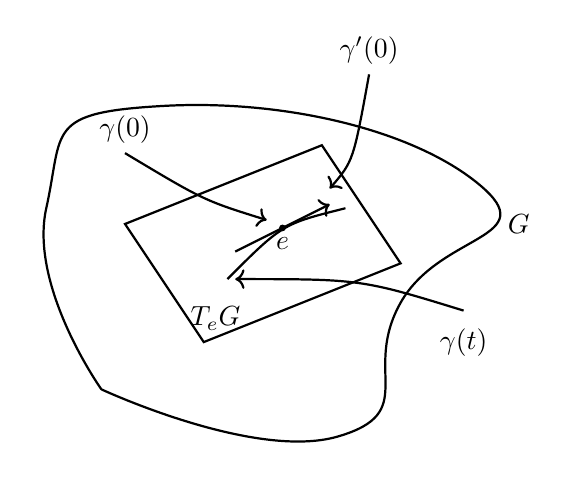
\begin{tikzpicture}
        
        % Draw the manifold G
        \draw[thick] plot [smooth,tension=1] 
        coordinates {(0.2,1.4) (3.2,0.8) (4,2.5) (5,4) (1,5) (-0.5,3.7) (0.2,1.4)};
        %\draw[thick] (0,0) to[out=30, in=180] (4,2.5) to[out=0, in=270] (5,4) to[out=90, in=30] (1,5) to[out=210, in=150] cycle;
        
        % Label G
        \node at (5.5,3.5) {$G$};
        
        % Draw the tangent space T_eG
        \draw[thick] (1.5, 2) -- (4, 3) -- (3, 4.5) -- (0.5, 3.5) -- cycle;
        
        % Label TeG
        \node at (1.65, 2.3) {$T_e G$};
        
        % Draw the curve \gamma(t)
        \draw[thick] (1.8, 2.8) .. controls (2.5, 3.5) .. (3.3, 3.7);
        
        % Label points and vectors
        \node at (0.5,4.7) {$\gamma(0)$};
        \draw[thick, ->] (0.5,4.4) .. controls (1.5,3.8) .. (2.3,3.55);
        \node at (4.8, 2) {$\gamma(t)$};
        \draw[thick, ->] (4.8,2.4) .. controls (3.5,2.8) .. (1.9,2.8);
        \filldraw[black] (2.5,3.45) circle (1pt) node[anchor=north] {$e$};
        \draw[thick, ->] (1.9, 3.15) -- (3.1, 3.75);
        \node at (3.6, 5.7) {$\gamma'(0)$};
        \draw[thick, ->] (3.6, 5.4) .. controls (3.4,4.3) .. (3.1,3.95);
        
    \end{tikzpicture}
\end{marginfigure}
由解的形式可见,对于$G$在幺元处的切空间$T_eG$的任意一个向量$A=\gamma'(0)$,就有$G$中的一元素$\gamma(1)=\exp(\gamma'(0))$与之对应.现在我们稍微总结一下:对于李群$G$这个流形,我们可以找到其单参数子群$T_eG$作为其切空间,并且我们可以找到一个指数映射从切空间到原空间,很快,当我们学会李代数的时候,我们会再次使用李代数的语言来总结:``李代数就是李群的切空间所导出的代数".

我们再次回到群$G$和它的单参数子群,我们发现,如果给定$G$中与幺元邻近的一个元素\sidenote[][]{当然,由于我们研究线性群,幺元为单位矩阵.}$g$,并定义向量$A=\log g$,则由$e^A=g$ 知,$A$ 为$G$ 在$e$ 处之切向量,$e^tA$为以 $A$ 为单位切向量的单参数子群.因此,对$G$ 中与幺元$e$ 邻近的一个元素就有$T_{e}(G)$($G$ 在幺元处的切空间)中一向量$A$ 与之对应,也就是说,设$U\subset G$ 中包含$e$ 的一个适当邻域,我们建立了一种对应关系
\begin{equation}
    \begin{aligned}
        G\supset U&\overunderset{\log}{\exp}{\longleftrightarrow}T_{e}(G)\\g&\to A=\log g\\e^{A}&\leftarrow A
    \end{aligned}
\end{equation}
这种对应关系可以使我们对李群的研究转化到与其对应的在幺元$e$处的切空间$T_e(G)$.而我们知道,$T_e(G)$是由向量组成的线性空间,其线性结构具有先天优势,拥有远比李群简单的结构和运算.但由于我们前面所提到的,由于矩阵乘法相比于数乘的不可交互性,自然由此导出的切空间的运算自然也不能简单用普通加减法来表述,即右侧关系图
\marginnote[]{$$\begin{aligned}&T_{e}(G)\qquad G\\&A\quad\longrightarrow\quad e^{A}\\&B\quad\longrightarrow\quad e^{B}\\&A+B\to e^{A+B}\ne e^{A}e^{B}\end{aligned}$$}

为此,我们迫切需要引入一种新的代数结构来反映$G$中的不可交换性,而具有这种新结构的线性空间$T_e(G)$
,就是我们下一节所要讲的\textbf{李代数}.
\section{李群与李代数}
\subsection{李代数}
由上面的讨论,我们现在知道$e^Ae^B\ne e^{A+B}$,那么,问题自然变为:$e^Ae^B=e^{?}$,或者表述为,$G$的单参数子群的代数结构是什么样的?

为了解决这个问题,我们设$A,B\in T_e(G)$,取一个参数$t$,并要求$|t|$适当小,从而能够保证$e^{tA}$与$e^{tB}$均为李群$G$中与幺元$e$邻近的元素\sidenote[][]{这个要求是必要的,我们需要满足后续使用级数的收敛性.}.现在我们构造一个函数:
\begin{equation}
    g(t)=e^{tA}e^{tB}e^{-tA}e^{-tB}
\end{equation}
显然,对于特例,即如果$e^{tA}$与$e^{tB}$可交换,$g(t)=e=\textbf{1}$,对于不可交换的情况,$g(t)$与幺元$e$的偏离程度反映了$e^{tA}$与$e^{tB}$的乘法与可交换的乘法之间的差异大小.现在我们具体分析$g(t)$.
\marginnote[]{展开的计算过程
$$\begin{aligned}
    g(t)& =e^{tA}e^{tB}e^{-tA}e^{-tB} \\
    &=(\textbf{1}+tA+\frac{t^{2}}{2!}A^{2}+\frac{t^{3}}{3!}A^{3}+\cdots)\\&\quad\times(\textbf{1}+tB+\frac{t^{2}}{2!}B^{2}+\frac{t^{3}}{3!}B^{3}+\cdots) \\&\quad\times(\textbf{1}-tA+\frac{t^2}{2!}A^2-\frac{t^3}{3!}A^3+\cdots)\\&\quad\times(\textbf{1}-tB+\frac{t^2}{2!}B^2-\frac{t^3}{3!}B^3+\cdots) \\
    &=\{\textbf{1}+t(A+B)+t^{2}(\frac{A^{2}}{2}+AB+\frac{B^{2}}{2})\\&\quad+t^{3}(\frac{A^{3}}{6}+\frac{A^{2}B}{2}+\frac{AB^{2}}{2}+\frac{B^{3}}{6})+O(t^{4})\} \\
    &\quad\{\textbf{1}-t(A+B)+t^2(\frac{A^2}{2}+AB+\frac{B^2}{2})\\&\quad-t^3(\frac{A^3}{6}+\frac{A^2B}{2}+\frac{AB^2}{2}+\frac{B^3}{6})+O(t^4)\} \\
    &=\textbf{1}+t(A+B-A-B)+t^{2}(AB-BA)+\\&\quad t^{3}(\frac{A^{2}B}{2}-\frac{AB^{2}}{2} \\
    &\quad-\frac{B^2A}{2}+\frac{BA^2}{2}-ABA+BAB)+O(t^4) \\
    &=\textbf{1}+t^{2}[A,B]+\frac{t^{3}}{2}([A,[A,B]]-[B,[B,A]])+O(t^{4})
\end{aligned}$$
}
\begin{equation}
    \begin{aligned}
        g(t)& =e^{tA}e^{tB}e^{-tA}e^{-tB} \\
        &=\textbf{1}+t^{2}[A,B]+\frac{t^{3}}{2}([A,[A,B]]-[B,[B,A]])+O(t^{4})
    \end{aligned}
\end{equation}
这里我们使用了对易子记号$[,]$,不过对于李代数,它也称为李括号,李乘法\sidenote[][]{事实上,对于线性群它等同于对易子,后面会加以区分的使用对易子和李括号.}.对于函数$g(t)$,我们有
\begin{equation}
    \frac{g(t)-\textbf{1}}{t^2}=[A,B]+O(t)
\end{equation}
因此,考虑极限$t\to0$时,
\begin{equation}
    \lim_{t\to0}\frac{g(t)-\textbf{1}}{t^{2}}=[A,B]
\end{equation}
由此,我们发现李群$G$的元素$e^{tA}$与$e^{tB}$的乘法的不可交换程度在$|t|$很小时主要取决于$[A,B]$

现在我们做变量代换$t=\sqrt{s}$,则
\begin{equation}
    \frac{g(\sqrt{s})-g(0)}{s}=[A,B]+O(\sqrt{s})
\end{equation}
并因此
\begin{equation}
    \lim_{s\to0}\frac{g(\sqrt{s})-g(0)}{s}=[A,B]
\end{equation}
这也说明$[A,B]$是李群$G$中过幺元的曲线$g(\sqrt{s})$在幺元处的\textbf{切向量},即$[A,B]\in T_e(G)$,这也意味着我们证明了如下关系
\begin{equation}
    \forall A,B\in T_{e}(G) , [A,B]\in T_{e}(G)
\end{equation}
即对易子(李括号)对向量空间$T_e(G)$的封闭性.


此时,我们可以回答开头所提到的问题了,不妨设$e^{tA}e^{tB}=e^{tC}$,则
\marginnote[]{展开的计算过程
$$\begin{aligned}
    tC&=\log e^{tC}=\log e^{tA}e^{tB}\\
    &=\log\{(\textbf{1}+t(A+B)+\frac{t^{2}}{2}(A^{2}+2AB+B^{2})+ \\
    &\quad+\frac{t^{3}}{6}(A^{3}+3A^{2}B+3AB^{2}+B^{3})+O(t^{4})\} \\
    &=t(A+B)+\frac{t^{2}}{2}(A^{2}+2AB+B^{2})\\&\quad+\frac{t^{3}}{6}(A^{3}+3A^{2}B+3AB^{2}+B^{3})+O(t^{4}) \\
    &\quad-\{t(A+B)+\frac{t^2}{2}(A^2+2AB+B^2)+O(t^3)\}^2/2+ \\
    &\quad+\{t(A+B)+\frac{t^{2}}{2}(A^{2}+2AB+B^{2})+O(t^{3})\}^{3}/3\\
    &\quad +O(t^{4}) \\
    &=t(A+B)+\frac{t^{2}}{2}(AB-BA)+\frac{t^{3}}{12}(A^{2}B-2ABA \\
    &\quad+BA^{2}-B^2A+BAB+BAB-AB^2)+O(t^4) \\
    &=(tA+tB)+\frac{1}{2}[tA,tB]\\
    &\quad+\frac{1}{12}[tA,[tA,tB]-tB,[tB,tA]]+O(t^{4}) 
\end{aligned}$$}
\begin{equation}
\begin{aligned}
    tC&=\log e^{tC}=\log e^{tA}e^{tB}\\
    &=(tA+tB)+\frac{1}{2}[tA,tB]+\frac{1}{12}[tA,[tA,tB]-tB,[tB,tA]]+O(t^{4}) 
\end{aligned}
\end{equation}
由此可见,只要给出李括号,$T_e(G)$中知道了与$e^{tA},e^{tB}$相对应的元素$tA,tB$即可求得$T_e(G)$中与$e^{tA}e^{tB}$相对应的元素.因此,我们认为李括号可以表述李群切空间的代数结构,并对于李括号有如右侧所示的性质.
\marginnote[]{李括号的性质$$\begin{gathered}
        \left\lbrack {A, A}\right\rbrack = 0\\
        \left\lbrack {A, B}\right\rbrack = - \left\lbrack {B, A}\right\rbrack\\
        \left\lbrack {A, c}\right\rbrack = 0\;\left( {c\text{ 只是一个数 }}\right)\\
        \left\lbrack {A + B, C}\right\rbrack = \left\lbrack {A, C}\right\rbrack + \left\lbrack {B, C}\right\rbrack\\
        \left\lbrack {A,{BC}}\right\rbrack = \left\lbrack {A, B}\right\rbrack C + B\left\lbrack {A, C}\right\rbrack\\
        \left\lbrack {A,\left\lbrack {B, C}\right\rbrack }\right\rbrack + \left\lbrack {B,\left\lbrack {C, A}\right\rbrack }\right\rbrack + \left\lbrack {C,\left\lbrack {A, B}\right\rbrack }\right\rbrack = 0
    \end{gathered}$$}

我们称有了李括号的向量空间$T_e(G)$构成一个李代数,更准确的来讲是李群$G$的李代数,并记为$\mathfrak{g}$.\\
李群的李代数完全刻画了李群在幺元附近的结构,而要研究李群在幺元附近的性质只需要研究李代数即可,但是需要注意的是,李代数\textbf{仅}刻画了李群在幺元附近的\textbf{局部}性质,\textbf{不能}反映其整体性质,一个李群对应一个李代数,而一个李代数可以对应多个李群.
\textbox{结构常数}{
设$G$是一个$r$维李群,取定幺元$e$的一个邻域$U$,在$U$中取定坐标系$\{U,\varphi\}$并取$e$为坐标原点:
\begin{equation}
    \varphi(e)=(0,0,\cdots,0)
\end{equation}
对于其的单参数子群,我们有
\begin{equation}
    \begin{cases}\gamma_j(t),&j=1,2,\cdots,r\\\varphi(\gamma_j(t))=(\underbrace{0,\cdots,0}_{(j-1)\text{个零}},t,0,\cdots,0)\end{cases}
\end{equation}
为其$r$条坐标曲线.

以$X_{j}= \gamma _{j}^{\prime }(0),j= 1, 2, \cdots , r$记为其在幺元处的切向量.即$X_j\in T_e(G) = \mathfrak{g}, j= 1, 2, \cdots , r$.显然,$\{X_1,X_2,\cdots,X_r\}$可取作为向量空间$T_{_e}(G)$的基——$T_{e}(G)$中任一向量可用它们的线性组合表出.由于$[X_i,X_j]\in \mathfrak{g}$,所以
\begin{equation}
    [X_{i},X_{j}]=\sum_{j,k=1}^{n}C_{ij}^{k}X_{k}\quad i,j=1,2,\cdots,r
\end{equation}
这$r^3$个数$\{C_{ij}^k\}k,i,j=1,2,\cdots,r$称为李群以$\{X_1,X_2,\cdots,X_r\}$,为基的\underline{结构常数}.
}
对于李代数$\mathfrak{g}$中任意向量$X,Y$,有
\begin{equation}
    \begin{aligned}
        X&=\sum_{j=1}^{r}\xi^{j}X_{j}&Y=\sum_{j=1}^{r}\eta^{j}X_{j}\\
        X&\sim(\xi^{1},\xi^{2},\cdots,\xi^{r})&Y=(\eta^{1},\eta^{2},\cdots\eta^{r})\\
        Z&=[X,Y]=\left[\sum_{j=1}^{r}\xi^{j}X_{j},\sum_{k=1}^{r}\eta^{k}X_{k}\right]&=\sum_{i=1}^{r}\sum_{j,k=1}^{r}C_{jk}^{i_{k}}\xi^{j}\eta^{k}X_{i}
    \end{aligned}
\end{equation}
将$Z$也用坐标表示
\begin{equation}
    Z=\sum_{i=1}^{r}\zeta^{ i}X_{i},\quad Z\sim(\zeta^{ 1},\zeta^{ 2},\cdots\zeta^{ r})
\end{equation}
此时易求出结构常数
\begin{equation}
    \zeta^{i}=\sum_{j,k=1}^{r}C_{jk}^{i}\xi^{j}\eta^{k},\quad i=1,2,\cdots,r
\end{equation}
由此可见,结构常数可以完全确定一个李代数.

需要强调的是,结构常数与基的选取有关,而李代数的一个重要的问题就是如何选取适当的基使结构常数最简单.\\
或许到此,你可能还对结构常数一头雾水,在再次讲解结构常数之前,我们还是先给出一些基本性质,并实际算一下结构常数.
\begin{equation}\label{1.43}
    \begin{aligned}
        &C_{ij}^{ k}=-C_{ji}^{ k}&i,j,k=1,2,\cdots,r\\
        &\sum_{l=1}^{r}\left(C_{ij}^{l}C_{lk}^{m}+C_{jk}^{l}C_{li}^{m}+C_{ki}^{l}C_{lj}^{m}\right)=0&i,j,k,m=1,2,\cdots,r.\end{aligned}
\end{equation}
\ytextbox{结构常数例子(1)}{
    我们再次考虑由例题给出的群$T_2=\Big\{\begin{bmatrix}e^{x_1}&x_2\\0&1\end{bmatrix}\Big|x_1,x_2\in\mathbb{R}\Big\}$,我们知道$\gamma_1(t)=\begin{bmatrix}e^t&0\\0&1\end{bmatrix} -\infty<t<\infty $与$\gamma_2(t)=\begin{bmatrix}1&t\\0&1\end{bmatrix} -\infty<t<\infty $是$T_2$的两个单参数子群,同时也是过幺元的两条曲线,我们给出在幺元处的切向量$X_1=\gamma_1'(0)=\begin{bmatrix}1&0\\0&0\end{bmatrix},X_2=\gamma_2'(0)=\begin{bmatrix}0&1\\0&0\end{bmatrix}$,因此李群$T_2$的李代数$\mathfrak{t}_2$的基由$X_1,X_2$组成,现在来求结构常数.
\begin{equation}
    \begin{aligned}&[X_1,X_1]=\begin{bmatrix}0&0\\0&0\end{bmatrix}\quad[X_2,X_2]=\begin{bmatrix}0&0\\0&0\end{bmatrix}\\&[X_1,X_2]=\begin{bmatrix}1&0\\0&0\end{bmatrix}\begin{bmatrix}0&1\\0&0\end{bmatrix}-\begin{bmatrix}0&1\\0&0\end{bmatrix}\begin{bmatrix}1&0\\0&0\end{bmatrix}=\begin{bmatrix}0&1\\0&0\end{bmatrix}=X_2.\end{aligned}
\end{equation}
所以,$C_{11}^1=C_{11}^2=C_{22}^1=C_{22}^2=0,\quad C_{12}^1=-C_{21}^1=0,\quad C_{12}^2=1,\quad C_{21}^2=-1.$
}
\ytextbox{结构常数例子(2)}{    我们再次回到$SO(3)$群,现在我们来求其李代数$\mathfrak{so}(3)$及其结构常数.\\
    我们列出其群元(绕$x,y,z$的转动),即旋转矩阵,如右侧所示
    \marginnote[*-3]{三个群元的矩阵表示:
        $$g_{x}(t)=\begin{bmatrix}1&0&0\\0&\cos t&-\sin t\\0&\sin t&\cos t\end{bmatrix}$$
        $$g_y(t)=\begin{bmatrix}\cos t&0&\sin t\\0&1&0\\-\sin t&0&\cos t\end{bmatrix}$$
        $$g_{z}(t)=\begin{bmatrix}\cos t&-\sin t&0\\\sin t&\cos t&0\\0&0&1\end{bmatrix}$$
    }
    
    此时,我们发现,这是其的三个单参数子群,而它们在幺元处的切向量一并给出
    \begin{equation}
        I_{1}=g_{x}'(0),\quad I_{2}=g_{y}'(0),\quad I_{3}=g_{z}'(0).
    \end{equation}
    于是$\{I_1,I_2,I_3\}$构成$SO(3)$的李代数$\mathfrak{so}(3)$的一组基,其李括号为:
    \begin{equation}
        [I_1,I_2]=I_1I_2-I_2I_1=I_3,[I_2,I_3]=I_1,[I_3,I_1]=I_2
    \end{equation}
    同时得出结构常数$C_{12}^{ 1}=0,C_{12}^{ 2}=0,C_{12}^{ 3}=1,\cdots.$
    
    我们可以发现,对于这个李括号,其还等价于三维欧式空间的向量乘法,我们就得到了简单情况下的李括号的退化情况.}


\subsection{李氏三定理}
在本节,我们将不加证明的叙述李氏三定理及上一节所得出的结构常数有什么作用.在$ r $维李群$ G $中,取幺元$ e $的邻域$ U $,并在其中选定一个坐标系$\{U,\varphi\}$,取$ e $为坐标原点,对于其中的乘法函数(回顾\ref{def:1.3}的定义)求导,定义辅助函数$l_{jk}$
\begin{equation}
    \begin{aligned}\frac{\partial z_j}{\partial y_k}|_{y_1,\cdots,y_r=0}&=\frac{\partial f_j\left(x_1,\cdots,x_r;y_1,\cdots,y_r\right)}{\partial y_k}|_{y_1,\cdots,y_r=0}\\&=l_{jk}\left(x_1,\cdots,x_r\right)\end{aligned}
\end{equation}
称$\{l_{jk}(x_1,\cdots,x_r)\}_{j,k=1,\cdots,r}$为李群$ G $的\textbf{辅助函数}.由此,我们发现只要知道辅助函数,就可以通过一组微分方程求出其乘法函数,进而确定李群$ G $的结构,即\textbf{李氏第一定理}.

进一步,对于辅助函数,我们可以证明存在微分方程组
\begin{equation}
    \begin{aligned}&\sum_{k=1}^r(l_{ki}(x)\frac{\partial l_{sj}(x)}{\partial x_k}-l_{kj}(x)\frac{\partial l_{si}(x)}{\partial x_k})=\sum_{k=1}^rC_{ij}^kl_{sk}(x)\\&\qquad s,i,j=1,2,\cdots,r.\end{aligned}
\end{equation}
这里$C_{ij}^k$即李群$ G $的李代数$\mf g$的结构常数,由此,李群的辅助函数完全由相应李代数的结构常数给定,已知结构常数就可解出辅助函数,并进一步给出乘法函数,即\textbf{李氏第二定理}.

一个李代数的结构常数满足\ref{1.43},反之已知一组数满足\ref{1.43}就可以构造出一个李代数,这组数就是这个李代数的结构常数,即\textbf{李氏第三定理}.

\begin{kaobox}[frametitle=李氏三定理]
    \begin{enumerate}
        \item \textbf{李氏第一定理}: 知道辅助函数,就可以通过一组微分方程求出其乘法函数,进而确定李群$ G $的结构
        \item \textbf{李氏第二定理}: 李群的辅助函数完全由相应李代数的结构常数给定,已知结构常数就可解出辅助函数,并进一步给出乘法函数
        \item \textbf{李氏第三定理}: 一个李代数的结构常数满足\ref{1.43},反之已知一组数满足\ref{1.43}就可以构造出一个李代数,这组数就是这个李代数的结构常数
    \end{enumerate}
\end{kaobox}


\section{几类李群及其应用}
\subsection{道路连通性问题}
事实上,对于$SU(2)$群的引入往往并没有那么显然,这一小节我们首先介绍一下简单的拓扑学中的概念,并以此解释对于$SU(2)$的引入的意义.
\begin{marginfigure}
    \centering
    \caption{连通区域$U$}
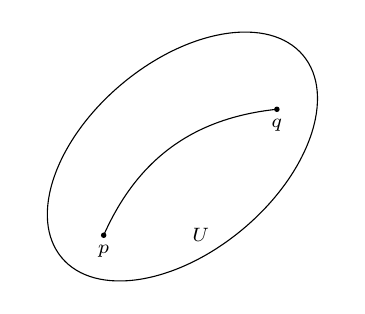
\begin{tikzpicture}
    \draw[rotate=40](0,0)ellipse(2 and 1.2);
    \path (-1, -1) edge [bend left] (1.2,0.6);
    \fill(1.2,0.6)circle(1pt)node[below]{\scriptsize\( q \)};
    \fill(-1, -1)circle(1pt)node[below]{\scriptsize\( p \)};
    %\draw[-latex,thick](-0.2,0.07)--(0.7,0.8)node[left,xshift=-0.1cm]{\scriptsize\( X \)};
    \node at(0,-1)[right]{\scriptsize\( U \)};
\end{tikzpicture}
\end{marginfigure}

对于一个区域$ U $,如果其中任意两点$p,q$都能由该区域内的点组成的曲线连接起来,那么我们称其为\textbf{道路连通}的.特殊的,对于满足过区域内任意一点$ p $的任意闭曲线$ L $,均可以\textbf{连续}的收缩到$ p $点,我们称这样的区域$ U $为\textbf{单连通}的.即如图中$ U $是单连通的,$ V $不是单连通的.
\begin{marginfigure}
    \centering
    \caption{非单连通区域$V$,$L_1$可以连续收缩回$ p $,但是$L_2$不能}
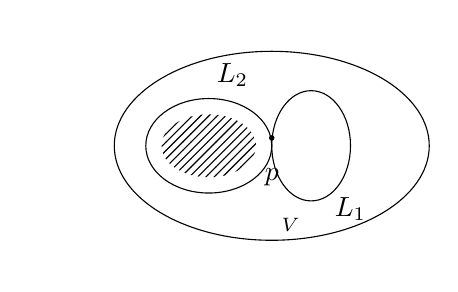
\begin{tikzpicture}
    % 绘制外层区域V
    \draw (-0.4,0) ellipse (2 and 1.2);
    \node at(-0.4,-1)[right]{\scriptsize\( V \)};
    
    % 绘制L1
    \draw (0.1,0) ellipse (0.5 and 0.7);
    \node at (0.6, -0.8) {$L_1$};
    
    % 绘制L2并填充斜线
    \begin{scope}
        \clip (-1.5,0) ellipse (2cm and 1.5cm);
        \fill[pattern=north east lines] (-1.2,0) ellipse (0.6cm and 0.4cm);
    \end{scope}
    \draw (-1.2,0) ellipse (0.8cm and 0.6cm);
    \node at (-0.9, 0.9) {$L_2$};
    
    % 绘制点p
    \fill (-0.4, 0.1) circle (1pt);
    \node at (-0.4, -0.4) {$p$};
\end{tikzpicture}
\end{marginfigure}
\subsubsection{$O(3)$群的道路连通性}
回忆$O(3)$群为3维正交群,其群元行列式为$\pm1$,首先假设存在这样的一条曲线$\gamma\in O(3)$,我们令这条曲线分别连接行列式为$+1$的群元$E_+$和行列式为$-1$的群元$E_-$,曲线自然被要求为连续的,其多项式函数:行列式自然同样被要求为连续的,但实际上行列式并不连续,自然得出$O(3)$\textbf{不是道路连通的}.

\subsubsection{$SO(3)$群的道路连通性}
既然$O(3)$不是道路连通的,那么我们继续考虑其特殊情况$SO(3)$群的情况.在前面,我们多次得出$SO(3)$可以表征$ 3 $维空间内的旋转,这自然吸引我们去使用更加形象化的表述去讨论其道路连通性.

我们在前面使用欧拉角给出过$SO(3)$的群元表达式
$$g=g_z^\alpha g_x^\beta g_z^\gamma$$

\begin{marginfigure}
    \centering
    \caption{$SO(3)$表征为球面,其中,$ p $与$ q $连接的曲线$\gamma_1$可以连续收缩到同一点,对于$ m,p,q,n $的任意除$m,n$的两两组合都满足这一关系,但是对于$m,n$两点,由于其关于球心对称,$ m $移动要求$ n $也需要同样对称的移动,故其始终保持一个大圆,不能收缩到同一点}
    \begin{tikzpicture}
        \def\R{2} % 切面半径
        \def\AngleGamma{0.1} % 极点倾斜角
        \fill[ball color=white] (0,0) circle (\R); % 3D 效果的球
        \coordinate[mark coordinate] (m) at (0,\R);
        \coordinate[mark coordinate] (n) at (0,-\R);
        \coordinate[mark coordinate] (p) at (\R*0.5,0.7);
        \coordinate[mark coordinate] (q) at (-\R*0.58,-0.3);
        \draw[rotate=20] (0,0.2) ellipse (1.2 and 0.7);
        \node at (0.6, 0.7) {$\gamma_1$};
        \node at (-0.5, -0.8*\R) {$\gamma_2$};
        \DrawLongitude{\R}{45};
        \node[above=8pt] at (m) {$m$};
        \node[below=8pt] at (n) {$n$};
        \node[below=8pt] at (p) {$p$};
        \node[below=8pt] at (q) {$q$};
    \end{tikzpicture}
\end{marginfigure}
其群元可以与一个三维空间内的单位球面建立起一一对应关系.另外,需要强调,关于球心对称的点应当视为同一类转动,于是对于图示情况,上面的曲线可以分类为$\gamma_1,\gamma_2$两类,一类可以连续收缩到同一点,另一类不行.于是我们称$SO(3)$为\textbf{双连通的}.

由于$SO(3)$为双连通的,为了寻找一个性质更好的群从而满足需求,这样我们便引入了单连通群$SU(2)$群.
\subsubsection{单连通群$SU(2)$}
对于$SU(2)$的群元$U$,存在其表示
\begin{equation}
    U=\begin{pmatrix}a&b\\-b^*&a^*\end{pmatrix}
\end{equation}
其中$a,b\in\mathbb C,aa^*+bb^*=1$,并且令$a=x_0+ix_1,b=x_2+ix_3$,存在关系
\begin{equation}
    x_0^2+x_1^2+x_2^2+x_3^2=1
\end{equation}
于是我们发现,$SU(2)$的群元$U$对应于四维空间$\mathbb R^4$中的三维球面$\mathbb S^3$上的一点,于是对于$SU(2)$连通性的研究可以转到对于三维球面$\mathbb S^3$的研究. 

对于$\bb S^3$,我们首先确定$x_0$,并且注意到当$x_0=\pm1$时为特殊情况,故先讨论$x_0\ne\pm1$.
\marginnote[]{分别对四个变量给定$$\begin{aligned}&x_{0}=\cos\frac{\theta}{2}\quad(0<\theta<360°)\\&x_{1}=\sin\frac{\theta}{2}\cos\alpha\\&x_{2}=\sin\frac{\theta}{2}\cos\beta\\&x_{3}=\sin\frac{\theta}{2}\cos\gamma\end{aligned} $$}我们给出了关于转轴$\mb n=(\cos\alpha,\cos\beta,\cos\gamma)$,转角$\theta$的关系.当我们取遍所有$x_0\ne\pm1$的点时,我们发现取到的区域占满了一个半径为$ 2 $个单位长度的\textbf{球体},但是球心和球面没有被取到.

对于$x_0=+1$时,其他变量均为$ 0 $,对应于球心,相应的,$x_0=-1$时对应于球面.显然,对于一个这样的球体,其为\textbf{单连通的}.
\subsubsection{$SU(2)$群与$SO(3)$群的2-1同态}
\marginnote[]{对于\textbf{同态}和\textbf{同构},如果两个群$G,G'$满足在映射$ f $下群乘法不变,即称$G,G'$是同态的,如果同态的同时还满足k-1映射,则称其为k-1同态.特别的,对于一一映射的情况,我们称$G,G'$是\textbf{同构}的.}
我们提到过,$SU(2)$是由于$SO(3)$群被引入的,在这一部分,我们将讨论二者之间的关联.

在量子力学中的学习,我们认识了\textbf{泡利矩阵},其相互正交,于是可以用来表示一个三维空间内的矢量$\mb{OP}=x\mb i+y\mb j+z\mb k$:
\begin{equation}
    P=x\sigma_x+y\sigma_y+z\sigma_z=\begin{pmatrix}z&x-\mathrm{i}y\\x+\mathrm{i}y&-z\end{pmatrix}
\end{equation}
显然$ P $是一个厄米矩阵,其迹为0\sidenote{回忆量子力学与线代知识,厄米矩阵即$U^\dagger=U$,求迹$\tr U$即主对角线求和.}.\\
取$SU(2)$的群元$Q$,对矩阵$ P $利用$ Q $构造相似矩阵$P'=QPQ^\dagger$,其可以表示为
\begin{equation}
    QPQ^\dagger=P^{\prime}=\begin{pmatrix}z^{\prime}&x^{\prime}-iy^{\prime}\\x^{\prime}+iy^{\prime}&-z^{\prime}\end{pmatrix}
\end{equation}
我们发现对于$x,y,z$与$x',y',z'$存在一个旋转矩阵$ R(\mb Q) $的变换,即在$SU(2)$和$O(3)$间建立了映射关系
\begin{marginfigure}
    \centering
    \caption{对应映射关系}
    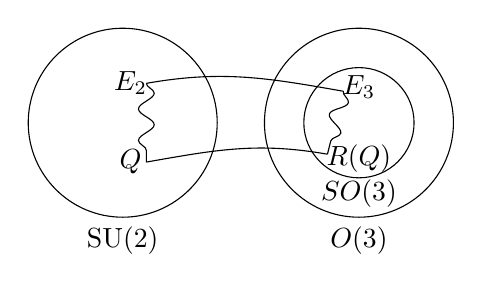
\begin{tikzpicture}
        \draw (0,0) ellipse (1.2cm and 1.2cm);
        \node at (0, -1.5) {SU(2)};
        \node at (0.1,0.5) {$E_2$};
        \node at (0.1,-0.5) {$\mb Q$};
        \draw (3,0) ellipse (1.2cm and 1.2cm);
        \node at (3, -1.5) {$O(3)$};
        \draw (3,0) ellipse (0.7cm and 0.7cm);
        \node at (3,-0.9) {$SO(3)$};
        
        \node at (3,0.45) {$E_3$};
        \node at (3,-0.45) {$R(\mb Q)$};
        \draw[-] (0.3,0.5) to [out=10,in=170] (2.8,0.4);
        \draw[-] (0.3,-0.5) to [out=10,in=170] (2.6,-0.4);
        \draw[decorate, decoration={snake, amplitude=1mm, segment length=4mm}] (0.3,0.5) -- (0.3,-0.5);
        \draw[decorate, decoration={snake, amplitude=1mm, segment length=4mm}] (2.8,0.4) -- (2.6,-0.4);
    \end{tikzpicture}
\end{marginfigure}
\begin{equation}
    \Map{R}{SU(2)}{O(3)}{\mb Q}{R(\mb Q)}
\end{equation}
考虑$\mb Q\maparrow R(\mb Q)$是连续的,且$SU(2)$是单连通群,于是$|R(\mb Q)|$是对于$\mb Q$的连续函数,并且对于幺元$|R(I_2)|=|I_3|=1$.因此,对于任意的$\mb Q\in SU(2)$,就有$R(\mb Q)\in SO(3)$

我们不加以证明的给出,单连通群$SU(2)$是双连通群$SO(3)$的一个\textbf{覆盖群}.这导致了费米子的半整数自旋,以及我们可以使用旋量表示电子.


\subsection{氢原子的$SO(4)$对称性}
虽然这一章侧重于数学内容的快速概览,但是适当结合一下物理应用是有益的,至少不会纠结这些东西究竟有什么用处.关于量子力学部分将会不再次介绍,默认读者已经了解这部分内容.

给定氢原子哈密顿量:$\displaystyle\hat{H}=\frac{\hat{\bm{p}^2}}{2\mu}-\frac{e^2}{r}$定义LRL矢量(拉普拉斯-龙格-楞次矢量,Laplace-Runge-Lenz矢量):
\begin{equation}
    \displaystyle \hat{\bm{A}}=\frac{1}{2\mu e^2}(\hat{\bm{p}}\times\hat{\bm{L}}-\hat{\bm{L}}\times\hat{\bm{p}})-\frac{\hat{\bm{r}}}{r}
\end{equation}
由对易关系$\displaystyle[\hat{L}_i,\hat{p}_j]=i\hbar \epsilon _{ijk}\hat{p}_k$,\sidenote{其中$\epsilon _{ijk}$为列维西维塔符号}将LRL矢量的分量写为
\begin{equation}
    \displaystyle\hat{A}_i=\frac{1}{2\mu e^2}\epsilon _{ijk}(\hat{p}_j\hat{L}_k-  \hat{L}_j\hat{p}_k)-\hat{n}_i   =\frac{1}{\mu e^2}\epsilon _{ijk}\hat{p}_j\hat{L}_k -\frac{i\hbar }{\mu e^2}\hat{p}_i-\hat{n}_i
\end{equation}
其中,$\displaystyle\hat{n}_i=\frac{\hat{r}_i}{r}$,相应有对易关系$[\hat{L}_i,\hat{n}_j  ]=i\hbar \epsilon _{ijk}\hat{n}_k $.计算LRL矢量的平方:
\begin{equation}
    \displaystyle\hat{\bm{A}^2}=\hat{A}_i \hat{A}_i =(\frac{1}{\mu e^2}\epsilon _{ijk}\hat{p}_j\hat{L}_k -\frac{i\hbar }{\mu e^2}\hat{p}_i-\hat{n}_i)(\frac{1}{\mu e^2}\epsilon _{ilm}\hat{p}_l\hat{L}_m -\frac{i\hbar }{\mu e^2}\hat{p}_i-\hat{n}_i)=\sum_{a=1}^{9}\hat{\Omega }  _a
\end{equation}

将括号展开得到$ 9 $项,形式比较复杂,需要熟悉掌握列维西维塔符号的使用,对于这个符号的介绍,请参考附录的内容.

分别计算,得出最终结果
\marginnote[]{
    利用了中心势场中$\hat{L}_k\hat{p}_k=\bm{\hat{L}}\cdot \bm{\hat{p}}=0$
$$\begin{align}\hat{\Omega }_1 &= \frac{1}{\mu ^2e^4}\epsilon _{ijk} \epsilon _{ilm}\hat{p}_j\hat{L}_k\hat{p}_l\hat{L}_m\\&=\frac{1}{\mu ^2e^4}(\delta _{jl}\delta _{km}-\delta _{jm}\delta _{kl})\hat{p}_j\hat{L}_k\hat{p}_l\hat{L}_m\\&= \frac{1}{\mu ^2e^4}(\hat{p}_j\hat{L}_k\hat{p}_j\hat{L}_k-\hat{p}_j \hat{L}_k\hat{p}_k \hat{L}_j)\\&=\frac{1}{\mu ^2e^4}\hat{p}_j\hat{L}_k\hat{p}_j\hat{L}_k\\&=\frac{1}{\mu ^2e^2}\hat{p}_j (i\hbar \epsilon _{kjl}\hat{p}_l+\hat{p}_j\hat{L}_k)\hat{L}_k\\&=\frac{1}{\mu ^2e^4}\hat{\bm{p}}^2\hat{\bm{L}} ^2    \end {align} $$
$$\begin{align}\hat{\Omega }_2 &=-\frac{i\hbar }{\mu ^2e^4}\epsilon _{ijk}\hat{p}_j\hat{L}_k\hat{p}_i \\& = -\frac{i\hbar }{\mu ^2e^4}\epsilon _{ijk}\hat{p}_j(i\hbar \hat{p}_m+\hat{p}_i \hat{L}_k  )\\&=\frac{\hbar ^2}{\mu ^2e^4}\epsilon _{ijk}\epsilon _{imk} \hat{p}_j\hat{p}_m-\frac{i\hbar }{\mu ^2e^4}\epsilon _{ijk}\hat{p}_j\hat{p}_i\hat{L}_k \\& =\frac{\hbar ^2}{\mu ^2e^4}(3\delta _{jm}- \delta _{jk}\delta _{mk}) \hat{p}_j\hat{p}_m\\& =\frac{2\hbar ^2}{\mu ^2e^4}\hat{\bm{p}}^2        \end {align} $$
$$\begin{align}\hat{\Omega }_3 &=-\frac{1}{\mu e^2}\epsilon _{ijk}\hat{p}_j\hat{L}_k\hat{n}_i\\& =-\frac{1}{\mu e^2}\epsilon _{ijk}\hat{p}_j(i\hbar \epsilon _{kim}\hat{n}_m+ \hat{n}_i\hat{L}_k) \\& =-\frac{i\hbar }{\mu e^2}\epsilon _{ijk}\epsilon _{kim} \hat{p}_j \hat{n}_m-\frac{1}{\mu e^2} \hat{p}_j\hat{n}_i\hat{L}_k\\& = -\frac{2i\hbar}{\mu e^2} \hat{p}_i\hat{n}_i-\frac{1}{\mu e^2} \frac{\hat{L}_k \hat{L}_k}{r}\\& =-\frac{2i\hbar}{\mu e^2}\hat{\bm{p}}\cdot  \hat{\bm{n}}-\frac{1}{\mu e^2}\frac{\hat{\bm{L}}^2}{r}     \end {align}$$
$$\begin{align}\hat{\Omega }_4 &=-\frac{i]\hbar }{\mu e^2}\epsilon _{ilm}\hat{p}_i\hat{p}_l\hat{L}_m=0      \end {align}$$
$$\begin{align}\hat{\Omega }_5=-\frac{\hbar ^2}{\mu'^2e^4}\hat{\bm{p}}^2        \end {align}$$
$$\begin{align}\hat{\Omega }_6=\frac{i\hbar }{\mu e^2}\hat{\bm{p}}\cdot  \hat{\bm{n}}         \end {align} $$
     这里利用了对易子$ \displaystyle[\hat{n}_i,\hat{p}_i]=i\hbar \frac{\partial }{\partial x_i}(\frac{x_i}{r} )=i\hbar \frac{2}{r}$
$$\begin{align}\hat{\Omega }_7&=\frac{i\hbar }{\mu e^2}\hat{n}_i\hat{p}_i  \\& =     \frac{i\hbar }{\mu e^2}([\hat{n}_i,\hat{p}_i]+\hat{p}_i\hat{n}_i)\\& =- \frac{\hbar^2 }{\mu e^2}\frac{2}{r} + \frac{i\hbar }{\mu e^2}\hat{p}_i\hat{n}_i\\& =- \frac{\hbar^2 }{\mu e^2}\frac{2}{r} + \frac{i\hbar }{\mu e^2}\hat{\bm{p}}\cdot \hat{\bm{n}}    \end {align} $$
$$\begin{align}\hat{\Omega }_8 &=-\frac{1}{\mu e^2}\epsilon _{ilm}\hat{n}_i\hat{p}_l\hat{L}_m \\& =-\frac{1}{\mu e^2}\frac{\hat{\bm{L}}^2 }{r}     \end {align} $$
$$\begin{align}\hat{\Omega }_9=\hat{n}_i \hat{n}_i=\bm{I}    \end {align} $$
    }
\begin{equation}
    \begin{align}\displaystyle \hat{\bm{A}^2} &=\sum_{a=1}^{9}\hat{\Omega }  _a \\& =\frac{1}{\mu ^2e^4}\hat{\bm{p}}^2\hat{\bm{L}}^2+\frac{\hbar ^2}{\mu ^2e^4}\hat{\bm{p}}^2-\frac{2}{\mu e^2}\frac{\hat{\bm{L}}^2}{r} - \frac{\hbar^2 }{\mu e^2}\frac{2}{r} +\bm{I} \\& =\frac{2}{\mu e^4}(\frac{\hat{\bm{p}}^2}{2\mu } \hat{\bm{L}}^2+\hbar ^2 \frac{\hat{\bm{p}}^2}{2\mu } - \frac{e^2}{r}\hat{\bm{L}}^2-\frac{e^2}{r}\hbar ^2 )+\bm{I} \\& =\frac{2}{\mu e^4}\hat{H}(\hat{\bm{L}}^2+\hbar ^2)+\bm{I} \end {align} 
\end{equation}
对于束缚态情况,$E<0$,将哈密顿量算符替换为$E$
\begin{equation}
    \displaystyle \hat{\bm{A}^2}=\frac{2E}{\mu e^4}(\hat{\bm{L}}^2+\hbar ^2)+\bm{I} 
\end{equation}
等价写为
\begin{equation}
    \displaystyle-\frac{\mu e^4}{2E}=- \frac{\mu e^4}{2E}\hat{\bm{A}}^2+ \hat{\bm{L}}^2+\hbar ^2=\hat{\bm{M}}^2+\hat{\bm{L}}^2+\hbar ^2
\end{equation}
其中,$\hat{\bm{M}} $是约化LRL矢量算符,定义为$\displaystyle\hat{\bm{M}}=\sqrt[]{-\frac{\mu e^4}{2E} }  \hat{\bm{A}}$,并且LRL矢量各分量对易关系为$\displaystyle[\hat{A}_i,\hat{A}_j ]=i\hbar (-\frac{2\hat{H} }{\mu e^4} )\epsilon _{ijk}\hat{L}_k $

于是得出
\begin{equation}
    \displaystyle[\hat{M}_i,\hat{M}_j ]=i\hbar \epsilon _{ijk}\hat{L}_k =[\hat{L}_i,\hat{L}_j]
\end{equation}
这样我们可以引入两个新的厄米算符把二者联系起来:$\displaystyle\hat{\bm{J}}_\pm =\frac{1}{2}(\hat{\bm{M}}\pm \hat{\bm{L}} )  $,验证其满足对易关系$[\hat{J}_{\pm i}, \hat{J}_{\pm j}]=i\hbar \epsilon _{ijk} \hat{J}_{\pm k};[\hat{J}_{+ i}, \hat{J}_{- j}]=0$.

我们称其为角动量算符,存在关系
\begin{equation}
    \displaystyle\hat{\bm{J}}^2_{+}= \hat{\bm{J}}^2_{-}=\frac{1}{4}(\hat{\bm{M}}^2+\hat{\bm{L}}^2) \pm \frac{1}{4}(\hat{\bm{M}}\cdot\hat{\bm{L}}+\hat{\bm{L}}\cdot \hat{\bm{M}}) 
\end{equation}
进而得出
\begin{equation}
    \displaystyle\hat{\bm{J}}^2_{+}= \hat{\bm{J}}^2_{-}=\frac{1}{4}(\hat{\bm{M}}^2+\hat{\bm{L}}^2) \qquad  \hat{\bm{M}}\cdot\hat{\bm{L}}+\hat{\bm{L}}\cdot \hat{\bm{M}}=0
\end{equation}
所以得到最后这个重要的结果
\begin{equation}
    \displaystyle-\frac{\mu e^4}{2E}=4\hat{\bm{J}}^2_++\hbar ^2  
\end{equation}
对于$\hat{\bm{J}}^2_+$的本征值,有
\begin{equation}
    \displaystyle\hat{\bm{J}}^2_+=j(j+1)\hbar^2 \qquad j=0,\frac{1}{2},1,\frac{3}{2},2,...
\end{equation}
氢原子中处于束缚态的电子具有的能级$ E $满足的代数方程为
\begin{equation}
    \begin{align}-\frac{\mu e^4}{2E(j)} &=4j(j+1)\hbar^2+\hbar ^2  \\&  =(4j^2+4j+1)\hbar^2\\& =(2j+1)^2\hbar^2\end{align}
\end{equation}
得到
$$\displaystyle E(j)=-\frac{\mu e^4}{\hbar^2}\frac{1}{2(2j+1)^2}\qquad j=0,\frac{1}{2},1,\frac{3}{2},2,...$$
即氢原子能级公式
\begin{equation}
    \displaystyle E_n=-\frac{\mu e^4}{\hbar^2}\frac{1}{2n^2}\qquad n=1,2,3,...
\end{equation}
对于$\hat{\bm{J}}_+$和$\hat{\bm{J}}_-$,回忆之前的李代数内容,不难发现其分别构成了$\mf{so}(3)$李代数,整体构成了$\mf{so}(4)=\mf{so}(3)\otimes\mf{so}(3)$李代数,即$SO(4)$对称性的来源,我们发现这种方法仅可以得到本征值,不能得到径向波函数的特征.
\subsection{再论氢原子: $\mf{so}(2,1)$李代数}
1




\section{流形与流形上的外微分}
\subsection{流形}
1
\section{纤维丛}
\subsection{切丛与余切丛}
1
\section{辛几何与辛结构}
\subsection{辛形式和辛流形}
1
\section{同调群}
\subsection{单纯复合形}
1
\section{De Rham 上同调群}
\subsection{流形上的De Rham 上同调群}
1
\section{仿射联络空间与黎曼流形}
\subsection{仿射联络}
1
















\setchapterpreamble[u]{\margintoc}
\chapter{场论初步}
\labch{intro}


从这一章开始,我们正式进入主题,也是真正核心的部分.现在开始每一章开头都会附带一段简单的小文章来快速总览部分内容,从而可以快速的建立对这些概念的朴素认知.
\section*{引子:最小作用量原理与路径积分}
\textit{我们都知道,数学上很讲究“公理”,希望一切都可以由公理自然给出,无论是欧几里得的平面几何几大公设还是近现代的ZFC公理系统,都试图为数学大厦建立一个夯实的根基,而这群搞物理的和搞数学又常常客串,自然而然,这些人也开始思考物理有没有所谓的公设,牛顿三定律?麦克斯韦方程组?薛定谔方程?爱因斯坦场方程?虽然这些定律都是正确的,但都在对应的能标下成立,谈不上“公理”.而最后,弄出来一些似是而非的东西,我们这一篇便讲其中之一:最小作用量原理.}\\
    \marginnote[]{\textbf{这里给出来自于陈童老师的从经典力学出发的视角:}\\
        最小作用量原理(principle of least action).按照最小作用量原理,粒子在相空间中不是按照哈密顿正则方程这样的微分方程演化,粒子是按“代价”最小的相空间路径演化.即是说,粒子的演化路径有无穷多种可能性,每一条可能的演化路径都要付出一个相应的“代价”,而粒子的真实演化路径是所有可能路径中“代价”最小的那条,严格一点说应该是“代价”取极值的那条(更严格地说应该是“代价”取驻值的那条,但是驻值这个概念比较微妙,为了使得读者更好理解,我们统一称作极值).每一条路径的“代价”就叫做这条路径的作用量.\\
        很显然,最小作用量原理看起来与哈密顿正则方程完全不同,结果却可以证明,这两种描述粒子在相空间中如何演化的方式物理上完全等价.哈密顿正则方程是一种局部视角的描述方式,每一个时刻都只需用到当前相点(相空间点) 局部邻域内的信息,因为微分方程中的求导运算只涉及邻域.而最小作用量原理是一种全局视角的描述方式,需要知道每一条可能路径的作用量这种全局信息.奇妙的是,这两种不同视角在物理上却是等价的.人们有时候将微分方程这样的局部视角称作蚂蚁视角(蚂蚁太小,每一只蚂蚁都只能看到一个很小的邻域),而将最小作用量原理这样的全局视角称作上帝视角.看待物理的蚂蚁视角源自于牛顿,正是牛顿想到用微分方程来描述物理规律.而上帝视角则源自于几何光学中的费马原理,然后经过莫培督(Maupertuis) 和哈密顿等人推广到力学里来.实际上,最小作用量原理有时候也称作哈密顿原理.不可思议的是,我们可以用这样两种完全不同的视角来看待同样的物理.\\不仅如此,这种局部视角和全局视角也都可以延伸到量子物理中,在量子力学中,局部视角大致会导致算符描述,而全局视角会导致路径积分描述.}
    \textit{而什么是最小作用量原理呢?正所谓水往低处流,水不会无缘无故的克服重力向上做功,它永远沿着做功最少的路径前进.对于我们中学就学过的电路来讲,导线会把电阻短路,因为电流自发的按照对外做功最小的路径前进.而这种按对外做功最小的行为,我们统称为最小作用量原理.作用量是系统拉格朗日量对时间的泛函(即函数的函数),而Wick转动告诉我们,实轴上的最小作用量原理就是虚时上的最小能量原理.\\
    我们知道,量子态和经典态是截然不同的,一个量子态经由某条路径(区分实际空间中的路径和概念上的路径)到达一个结果的量子态的传播过程并不能像经典的时候那样直接表述出来:我们只知道起始时刻的位置和终点时刻的位置,中间的过程也不是传统意义上的移动,而是黑箱一般,经过一定时间之后就转移到终点,中间的过程是未知的.\\
    于是,我们的首要目的就是破解这个黑箱,对于初态和末态,我们定义了一个新的算符:传播子来代表这个黑箱过程.而下一刻粒子出现在末态的概率幅依赖于始末位置间的所有路径,但是我们知道,两点间可能有无数种方式路径,但那又如何?费曼提出了路径积分,将所有可能的路径全部积分一遍.其遵循了一些简朴的思想:对于过多扭曲的路径,我们可以认为反复的部分的平均为0,自然也不必考虑扭曲转圈的情况,路径被统一为单行线.而始末位置的连线则是经典路径,所有扭曲的其他路径都要以经典路径为核心,偏离太远的也被近似为0.\\
    我们此时从最小作用量原理来解释这个朴素的思想:存在无穷多可能的路线,但是大部分都是高阶项,这说明我们可以取最少的路径来表述这个过程,作用量相当于不同路径的权重,最小作用量原理要求总体权重和最小,这意味着需要有效路径最少,也对应着之前所遵循的原理.\\
    另外需要强调的是,一次量子化(量子力学)告诉我们应当使用波来描述粒子,二次量子化又重新使用粒子来描述波,这些虽然符合实验现象,但是对于某些情况就捉襟见肘了.路径积分时区别于那两种的表述方法,它认为需要使用场来表述粒子,其构建了场论形式的泛函积分方法.}
\section{路径积分}
在初等量子力学的学习中,我们在经典量子化的框架内进行表述,在本节,我们将初步探索另一种表述方法:\textbf{路径积分法}.
\subsection{量子系统与经典系统中的路径积分}
我们采取通过一个最基本物理图像的方式来引入路径积分:考虑一维空间内的一个有质量$ m $的粒子,其动力学可以通过拉格朗日量来表述:\sidenote[][]{本章开始采取这类更加清晰的公式标注方法.}\\

\begin{equation}
    \vspace{\baselineskip}
    L(q,\dot{q})=\tikzmarknode{1eq1}{\highlight{red}{$\frac12m\dot{q}^2$}}-\tikzmarknode{1eq2}{\highlight{blue}{$V(q)$}}
\end{equation}
\begin{tikzpicture}[overlay,remember picture,>=stealth,nodes={align=left,inner ysep=1pt},<-]
    % 对于 "1" 定位点
    \path (1eq1.north) ++ (0,2em) node[anchor=south east,color=red!67] (eq1/1){\textbf{动能项}};
    \draw [color=red!87](1eq1.north) |- ([xshift=-0.3ex,color=red]eq1/1.south west);
    % 对于 "2" 定位点
    \path (1eq2.south) ++ (0,-1.5em) node[anchor=north west,color=blue!67] (eq1/2){\textbf{势能项}};
    \draw [color=blue!57](1eq2.south) |- ([xshift=-0.3ex,color=blue]eq1/2.south east);
\end{tikzpicture}

并假设粒子位于与时间无关的势$ V(q) $中.我们使用广义坐标$ q $来表述粒子的位置\sidenote[][]{广义坐标往往指一组无关联约束的坐标,即对于三维坐标表述,如果$x,y,z$之间没有约束方程,那么$x,y,z$就可以认为是一组广义坐标.不过,目前可以仅把它们当做特殊的坐标/动量(对于广义动量).},对于广义坐标,同样有$\dot{q}=\partial_t q$.于是,根据我们在理论力学中所学到的欧拉-拉格朗日方程
\begin{equation}
    \frac{\d}{\dt}\frac{\partial L(q,\dot{q})}{\partial\dot{q}}=\frac{\partial L(q,\dot{q})}{\partial q}\quad\text{也就是}\quad m\ddot{q}=-\frac{\partial V(q)}{\partial q}.
\end{equation}
同时,我们考虑由下式定义的\textbf{哈密顿量}$H(p,q)$
\begin{equation}
    H(p,q)=p\dot{q}-L(q,\dot{q})=\frac{p^2}{2m}+V(q)\quad\text{其中广义坐标被定义为}\quad p=\frac{\partial L(q,\dot{q})}{\partial\dot{q}}=m\dot{q}
\end{equation}
我们于是通过哈密顿量给出该粒子的经典动力学关系(特别强调的一点是,在对哈密顿量偏导时,我们认为广义坐标和广义动量是无关联的.):
\begin{equation}
    \dot{p}=-\frac{\partial H(p,q)}{\partial q}=-\frac{\partial V(q)}{\partial q},\dot{q}=\frac{\partial H(p,q)}{\partial p}=\frac{p}{m}
\end{equation}

在量子力学中,我们把广义坐标和广义动量的关系上升至对易关系(后续我们把广义坐标和广义动量简称为坐标和动量).
\begin{equation}
    [\hat{q},\hat{p}]=i\hbar
\end{equation}
同时经典变量$A(p,q)$同时上升为算符$\hat{A}\equiv A(\hat{p},\hat{q})$自然经典哈密顿量也变为量子哈密顿量方程.
\begin{equation}
    \hat{H}=\frac{\hat{p}^2}{2m}+V(\hat{q})
\end{equation}


我们知道系统的物理态由希尔伯特空间$ \mathcal H $中的态矢量$|\psi(t)\ra$所描述,我们使用薛定谔方程来描述态矢量的时间演化:\\

\begin{equation}
    \vspace{\baselineskip}
    %公式编号: 7
    \tikzmarknode{7eq1}{\highlight{red}{$i\hbar\partial_t$}}|\psi(t)\rangle=\tikzmarknode{7eq2}{\highlight{blue}{$\hat{H}$}}|\psi(t)\rangle
\end{equation}
\begin{tikzpicture}[overlay,remember picture,>=stealth,nodes={align=left,inner ysep=1pt},<-]
    % 对于 "1" 定位点
    \path (7eq1.north) ++ (0,2em) node[anchor=south east,color=red!67] (eq7/1){\textbf{能量$ E $}};
    \draw [color=red!87](7eq1.north) |- ([xshift=-0.3ex,color=red]eq7/1.south west);
    % 对于 "2" 定位点
    \path (7eq2.south) ++ (0,-1.5em) node[anchor=north west,color=blue!67] (eq7/2){\textbf{哈密顿量算符}};
    \draw [color=blue!57](7eq2.south) |- ([xshift=-0.3ex,color=blue]eq7/2.south east);
\end{tikzpicture}

我们熟知我们可以利用时间演化算符$\hat U$写成方程的解:
\begin{equation}
    |\psi(t)\rangle=\hat{U}(t)|\psi(t=0)\rangle,\quad i\hbar\partial_t\hat{U}(t)=\hat{H}\hat{U}(t).
\end{equation}
由于哈密顿量与时间无关,所以我们可以写成时间演化算符的表示
\begin{equation}
    \hat{U}(t)=e^{-\frac i\hbar\hat{H}t}
\end{equation}
在这里,我们重申一点:给定时空位置的波函数代表了该粒子位于该时空位置的概率振幅.\\
同时我们写出\\\\\\

\begin{equation}
    \vspace{\baselineskip}
    %公式编号: 10
    \tikzmarknode{10eq1}{\highlight{red}{$\psi(q_f,t_f)$}}=\langle q_f|\psi(t_f)\rangle=\langle q_f|\hat{U}(t_f-t_i)|\psi(t_i)\rangle=\int \dq_iU(q_f,q_i;t_f-t_i)\tikzmarknode{10eq2}{\highlight{blue}{$\psi(q_i,t_i)$}}
\end{equation}
\begin{tikzpicture}[overlay,remember picture,>=stealth,nodes={align=left,inner ysep=1pt},<-]
    % 对于 "1" 定位点
    \path (10eq1.north) ++ (0,2em) node[anchor=south west,color=red!67] (eq10/1){\textbf{$ t_f $时刻时粒子位于$q_f$的概率}};
    \draw [color=red!87](10eq1.north) |- ([xshift=-0.3ex,color=red]eq10/1.south east);
    % 对于 "2" 定位点
    \path (10eq2.south) ++ (0,-1.5em) node[anchor=north east,color=blue!67] (eq10/2){\textbf{$ t_i $时刻时粒子位于$q_i$的概率}};
    \draw [color=blue!57](10eq2.south) |- ([xshift=-0.3ex,color=blue]eq10/2.south west);
\end{tikzpicture}

其中$U(q_f,q_i;t_f-t_i) = \langle q_f|\hat{U}(t_f-t_i)|q_i\rangle $被称为传播子,其表示了这个粒子在$t_f-t_i$时间内从位置$q_i$传播到位置$q_f$的概率振幅.并且若已知哈密顿量$\hat{H}$本征态$\{|n\ra,\epsilon_n\}$,那么我们以此可以把传播子写作
\begin{equation}
    \begin{aligned}U(q_f,q_i;t_f-t_i)&=\langle q_f|e^{-\frac{i}{\hbar}\hat{H}(t_f-t_i)}|q_i\rangle=\sum_n\langle q_f|n\rangle e^{-\frac{i}{\hbar}\epsilon_n(t_f-t_i)}\langle n|q_i\rangle\\[2ex]&=\sum_ne^{-\frac{i}{\hbar}\epsilon_n(t_f-t_i)}\varphi_n(q_f)\varphi_n^*(q_i)\end{aligned}
\end{equation}
其中$\varphi_n(q)=\la q|n\ra$为坐标表象下的波函数.我们发现传播子给出了关于这个哈密顿量的波函数和能级的全部信息,这也意味着我们可以把求解波函数的问题变为求解这个哈密顿量所对应的传播子的问题.
\subsection{路径积分初步}
我们刚刚发现了通过求解传播子可以间接求解波函数,而现在的问题是:如何求出传播子? 这里我们用到费曼的路径积分方法,我们先来首先说明\textbf{传播子可以写为路径积分的形式}.

我们首先考虑一个充分短的时间$\epsilon$

\begin{equation}
    \vspace{\baselineskip}
    %公式编号: 12
    U(q_f,q_i;\epsilon)=\langle q_f|e^{-i\hat{H}\epsilon}|q_i\rangle \tikzmarknode{12eq2}{\highlight{blue}{$\simeq$}}\langle q_f|e^{-i\epsilon\frac{\hat{p}^2}{2m}}e^{-i\epsilon V(\hat{q})}|q_i\rangle
\end{equation}
\begin{tikzpicture}[overlay,remember picture,>=stealth,nodes={align=left,inner ysep=1pt},<-]
    % 对于 "2" 定位点
    \path (12eq2.south) ++ (0,-1.5em) node[anchor=north east,color=blue!67] (eq12/2){\textbf{Baker–Hausdorff规则$e^{\epsilon\hat{A}+\epsilon\hat{B}}=e^{\epsilon\hat{A}}e^{\epsilon\hat{B}}e^{\mathcal{O}(\epsilon^{2})}$}};
    \draw [color=blue!57](12eq2.south) |- ([xshift=-0.3ex,color=blue]eq12/2.south west);
\end{tikzpicture}

我们在其中插入一个单位算符的谱分解\sidenote[][]{此时已经开始采取自然单位制了(对单位制可以参考附录).},在下面的式子中,我们使用了归一化假设$\la q|p\ra=L^{-1/2}e^{ipq}\;q\in[0,L]$,$ q $为连续的位置变量,而$p=n\frac{2\pi}L\;n\in \mathbb Z$为离散的动量变量(关于边界$ L $,并且有归一化条件$e^{ipL}=1$),在极限$L\to\infty$,存在$\frac1L\sum_p\to\int_{-\infty}^\infty\frac{\d p}{2\pi}$.\\
于是,式子变为
\begin{equation}
    \vspace{\baselineskip}
    %公式编号: 13
    \begin{aligned}
        U(q_f,q_i;\epsilon)& \begin{aligned}&=\sum_p\langle q_f|e^{-i\epsilon\frac{\hat{p}^2}{2m}}|p\rangle\langle p|e^{-i\epsilon V(\hat{q})}|q_i\rangle\end{aligned} \\
        &=\int\frac{\d p}{2\pi}\exp\biggl\{-i\epsilon\biggl[\frac{p^2}{2m}+V(q_i)\biggr]+ip(q_f-q_i)\biggr\} \\
        &\tikzmarknode{13eq2}{\highlight{blue}{$=$}}\bigg(\frac{m}{2\pi i\epsilon}\bigg)^{1/2}\exp\bigg\{i\epsilon\bigg[\frac{m}{2}\frac{(q_{f}-q_{i})^{2}}{\epsilon^{2}}-V(q_{i})\bigg]\bigg\}.
    \end{aligned}
\end{equation}
\begin{tikzpicture}[overlay,remember picture,>=stealth,nodes={align=left,inner ysep=1pt},<-]
    % 对于 "2" 定位点
    \path (13eq2.south) ++ (0,-1.5em) node[anchor=north west,color=blue!67] (eq13/2){\textbf{此处计算需要利用留数定理,附录中给出了mma计算代码}};
    \draw [color=blue!57](13eq2.south) |- ([xshift=-0.3ex,color=blue]eq13/2.south east);
\end{tikzpicture}

为了使对$ p $的积分收敛,我们假设$\epsilon$包含一个小的负虚部,我们发现,指数上的部分恰好是$ i $乘以无穷小作用量$S(q_f,q_i;\epsilon)$,不难发现这个作用量对应着无穷小时间$\epsilon$内$ q_i $和$ q_f $之间以恒定速度的直线路径,于是,我们把式子写为如下形式:
\begin{equation}\label{4eq14}
    U(q_f,q_i;\epsilon)=\left(\frac{m}{2\pi i\epsilon}\right)^{1/2}e^{iS(q_f,q_i;\epsilon)+\mathcal{O}(\epsilon^2)}
\end{equation}
仅有无穷小时间间隔的传播子显然是远远不够的,现在我们想计算出任意时间间隔$t_f-t_i$的传播子$U(q_f,q_i;t_f-t_i)$.我们考虑将时间段$t_f-t_i$分割为$ N $个长为$\epsilon=(t_f-t_i)/N$的等大小的部分,只要最终我们取极限$N\to\infty\;(\epsilon\to0)$,并对全部时间步积分,就得到了任意时间间隔$t_f-t_i$的传播子.
\begin{equation}
    \begin{aligned}
        \begin{aligned}U(q_f,q_i;t_f-t_i)\end{aligned}& \begin{aligned}=\langle q_{f}|e^{-i\hat{H}\epsilon}\cdots e^{-i\hat{H}\epsilon}|q_{i}\rangle\end{aligned} \\
        &=\int\prod_{k=1}^{N-1}\d q_k\langle q_f|e^{-i\hat{H}\epsilon}|q_{N-1}\rangle\langle q_{N-1}|e^{-i\hat{H}\epsilon}|q_{N-2}\rangle\cdots\langle q_1|e^{-i\hat{H}\epsilon}|q_i\rangle \\
        &=\int\prod_{k=1}^{N-1}\d q_k\prod_{k=1}^NU(q_k,q_{k-1};\epsilon)
    \end{aligned}
\end{equation}
其中$q_0=q_i,q_N=q_f$,在\ref{4eq14}中,我们对每个时间步传播子都忽略了$\epsilon^2$的高阶项,对于整体,其导致了阶为$\epsilon$的总误差. \\
现在我们继续考虑,令$N\to\infty$我们有
\begin{equation}
    U(q_f,q_i;t)=\lim_{N\to\infty}\left(\frac{mN}{2\pi it}\right)^{N/2}\int\prod_{k=1}^{N-1}\d q_k e^{iS[q]}
\end{equation}
其中作用量为
\begin{equation}
    S[q]=\sum_{k=1}^NS(q_k,q_{k-1};\epsilon)=\epsilon\sum_{k=1}^N\left[\frac m2\frac{(q_k-q_{k-1})^2}{\epsilon^2}-V(q_{k-1})\right]
\end{equation}
在极限$N\to\infty$,我们可以把求和写做积分:
\begin{equation}
    \begin{aligned}\epsilon\sum_{k=1}^N\frac{m}{2}\frac{(q_k-q_{k-1})^2}{\epsilon^2}&\to\int_{t_i}^{t_f} \d t\frac{m}{2}\dot{q}^2\\\epsilon\sum_{k=1}^NV(q_{k-1})&\to\int_{t_i}^{t_f} \d t V(q)\end{aligned}
\end{equation}
我们使用$q(t)$表示这个粒子的``路径"(trajectory),对于始末位置$q(t_i)=q_i,q(t_f)=q_f$,但这并不意味着在大$ N $极限下的连续性/可微性.我们定义积分测度为如下形式\sidenote[][]{我们可以认为这个形式不过是把一些成套的东西包装成一个微分算符,依赖这种写法,可以简化我们对于路径积分的表述.}:
\begin{equation}
    \mathcal{D}[q]=\lim_{N\to\infty}\left(\frac{mN}{2\pi i\hbar t}\right)^{N/2}\prod_{k=1}^{N-1}\d q_k
\end{equation}
于是传播子可以简化为
\begin{equation}
    U(q_f,q_i;t_f-t_i)=\int_{q(t_i)=q_i}^{q(t_f)=q_f}\mathcal{D}[q]e^{\frac{i}{\hbar}S[q]}
\end{equation}
同时作用量被定义为

\begin{equation}
    \vspace{\baselineskip}
    %公式编号: 21
    \tikzmarknode{21eq1}{\highlight{red}{$S[q]$}}=\int_{t_i}^{t_f}\d t\tikzmarknode{21eq2}{\highlight{blue}{$L(q,\dot{q})$}}
\end{equation}
\begin{tikzpicture}[overlay,remember picture,>=stealth,nodes={align=left,inner ysep=1pt},<-]
    % 对于 "1" 定位点
    \path (21eq1.north) ++ (0,2em) node[anchor=south east,color=red!67] (eq21/1){\textbf{作用量}};
    \draw [color=red!87](21eq1.north) |- ([xshift=-0.3ex,color=red]eq21/1.south west);
    % 对于 "2" 定位点
    \path (21eq2.south) ++ (0,-1.5em) node[anchor=north west,color=blue!67] (eq21/2){\textbf{拉格朗日量}};
    \draw [color=blue!57](21eq2.south) |- ([xshift=-0.3ex,color=blue]eq21/2.south east);
\end{tikzpicture}

现在我们发现,这个作用量的形式与路径$q(t)$的经典作用量的形式一致.

我们不难注意到:积分测度$\mathcal D$中包含的极限是\textbf{发散的},在处理发散问题之前,我们首先尝试讨论其物理含义:对于传播子,我们从公式角度出发观察传播子的形式,我们不难发现这个积分过程只规定了初值条件(初态位置和时间以及末态位置和时间),我们需要对\textbf{所有可能的}路径进行积分(或者说是求和,这两者并没有太大区别),并且对于求和过程,我们最后得出的答案是依赖于作用量的对每条路径的\textbf{加权和}.而按照物理情景的解释,我们有``当一个物理过程\sidenote[][]{我们并没有区别宏观和微观,这是因为其对宏观仍然适用,但由于对应原理,我们不必对宏观现象如此分析.}可以以多种路径进行时,它的概率幅由每种路径的幅值之和给出\sidenote[][]{英文原文:When a
    process can take place in more than one way, its probability amplitude is given by the
    sum of the amplitudes for each way.}".

但是,我们发现这并没有解决发散问题,于是我们要求路径是足够``好"的.即要求动力学项$[q(t+\epsilon)-q(t)]^2/\epsilon$在极限$\epsilon\to0$时收敛,并认为在不满足这个条件的路径会剧烈震荡,其平均值为$ 0 $,即不那么``好"的路径.事实上,这种方法似乎完全看不出来严格的数学依据,但现实如此(这里可以引用那些经典的物理小笑话了,至少我们目前不用去思考如何把这些东西严谨化.)\sidenote[][]{关于这一大段的文字讨论是必须的,其有助于构建量子场论的物理图景,事实上,在这一章我一直在尝试把更多重点放在公式内部并突出显示它,倘若把重点置于一大堆文字中,读者不加以仔细的阅读的话,便很容易错过去.而且,对于物理这一门学科,过于长段的文字很难真的揭示什么内涵,它们往往起到解释公式的作用,或者说,公式才是文章的主体.同样的,这一大段内容我放在了脚注中,同样为了让人们去注意到它.}.

\subsubsection{经典极限}
或许你们发现在上一部分的结尾中,我们并没有像往常一样去省略约化普朗克常数$\hbar$,这有关于经典极限的讨论.

我们所关注的重点路径为``贴近"经典路径的路径,其作用量是静态的.
\begin{equation}
    \left.\frac{\delta S[q]}{\delta q(t)}\right|_{q=q_c}=0
\end{equation}
对于非静态的路径,其意味着作用量的大幅振荡,其平均值为0,或者说,更准确的,传播子$U(q_f,q_i;t_f-t_i)$由路径$q(t)$所主导,其作用量$S[q]$与经典作用量$S_c=S[q_c]$相差一个$\hbar$阶项:$|S-S_c|\lesssim\hbar$.当$|S_c|\gg\hbar $时,这些路径非常接近经典作用量的路径.而对于相反的极限中,同样满足条件$|S-S_c|\lesssim\hbar$的路径就与经典作用量导致的路径截然不同.于是,形式上的经典极限对于与$\hbar\to0$的极限.

\begin{remark}
    \textit{为了得到极限$\hbar\to0$中的传播子,我们写出$q(t)=q_c(t)+r(t)$(我们假设仅存在唯一一条经典轨道.),并把作用量对于$r(t)$展开到第二阶.}
    \begin{equation}
        \begin{aligned}&U(q_f,q_i;t_f-t_i)\\&\simeq e^{\frac{i}{\hbar}S[q_c]}\int_{r(t_i)=0}^{r(t_f)=0}\mathcal{D}[r]\exp\biggl\{\frac{i}{2\hbar}\int_{t_i}^{t_f}\d t \d t' \frac{\delta^2S[q]}{\delta q(t)\delta q(t')}\biggr|_{q=q_c}r(t)r(t')\biggr\}\end{aligned}
    \end{equation}
    \textit{这类积分被称为\textbf{高斯积分},高斯积分并不需要你去思考如何巧妙积分出来,仅需套用公式就能得出答案,而对应的积分表全部列在下面,即式\ref{GaussIntegral}.}
    \begin{equation}
        U(q_f,q_i;t_f-t_i)\simeq e^{\frac{i}{\hbar}S[q_c]}\det\left(\frac{1}{2\pi i\hbar}\frac{\delta^2S[q]}{\delta q(t)\delta q(t')}\bigg|_{q=q_c}\right)^{-1/2}
    \end{equation}
    \textit{我们最后得到的结果所遵循的过程被称为稳态相位近似.}
\end{remark}
\subsubsection{高斯积分表}
如下表,其中$ K $是对称矩阵.
\begin{equation}\label{GaussIntegral}
    \begin{aligned}
        &\int_{-\infty}^{+\infty} e^{-\frac{1}{2}ax^{2}}\dx=\sqrt{\frac{2\pi}{a}} 
        &&\int_{-\infty}^{+\infty}x^{2n}e^{-\frac12ax^2}\dx=\sqrt{2\pi}a^{-\frac{2n+1}2}(2n-1)!! \\
        &\int_{-\infty}^{+\infty}e^{-\frac12ax^2+Jx}\dx=\sqrt{\frac{2\pi}a}e^{\frac{J^2}{2a}} 
        &&\int_{-\infty}^{+\infty} e^{-\frac{1}{2} ax^{2}+iJx} \dx=\sqrt{\frac{2\pi}{a}}e^{-\frac{J^{2}}{2a}} \\
        &\int_{-\infty}^{+\infty}e^{i(\frac{1}{2}ax^{2}+Jx)}\dx=\sqrt{\frac{2\pi i}{a}}e^{-i\frac{J^{2}}{2a}} 
        &&\int_{-\infty}^{+\infty}e^{-\frac{1}{2}x^{T}Kx}\d^{n}x=\sqrt{\frac{(2\pi)^{n}}{\det K}} \\
        &\int_{-\infty}^{+\infty}e^{-\frac{1}{2}x^{T}Kx+Jx}\d^{n}x=\sqrt{\frac{(2\pi)^{n}}{\det K}}e^{\frac{1}{2}JK^{-1}J} 
        &&\int_{-\infty}^{+\infty}e^{-\frac{1}{2}x^{T}Kx+iJx}\d^{n}x=\sqrt{\frac{(2\pi)^{n}}{\det K}}e^{-\frac{1}{2}JK^{-1}J} \\
        &\int_{-\infty}^{+\infty}e^{i(\frac{1}{2}x^{T}Kx+Jx)}\d^{n}x=\sqrt{\frac{(2\pi i)^{n}}{\det K}}e^{-\frac{i}{2}JK^{-1}J}
    \end{aligned}
\end{equation}
需要强调的是,虽然看似高斯积分较为复杂,但都处于高等数学范畴内的积分,如需要记忆的话也可以仅记忆下面这个,其他都可以通过简单的系数替换得到:
\begin{equation}
    \int_{-\infty}^{+\infty}e^{-\frac12ax^2+Jx}\dx=\sqrt{\frac{2\pi}a}e^{\frac{J^2}{2a}}
\end{equation}
\subsubsection{时序算符以及哈密顿量}
对于海森堡绘景下算符的矩阵元,例如算符$\hat{q}(t)=e^{i\hat{H}t}\hat{q}e^{-i\hat{H}t}$
\begin{equation}
    \langle q_f,t_f|\hat{q}(t)|q_i,t_i\rangle=\langle q_f|e^{-i\hat{H}(t_f-t)}\hat{q}e^{-i\hat{H}(t-t_i)}|q_i\rangle 
\end{equation}
如之前那样,我们将时间间隔无限拆分并再次积分,就可以得到矩阵元的路径积分表示:
\begin{equation}
    \langle q_f,t_f|\hat{q}(t)|q_i,t_i\rangle=\int_{q(t_i)=q_i}^{q(t_f)=q_f}\mathcal{D}[q] q(t)e^{iS[q]}
\end{equation}
而为了使用路径积分表示两个不同时间的算符的乘积,我们引入一个新算符,其被定义为\\

\begin{equation}
    \vspace{\baselineskip}
    %公式编号: 29
    \tikzmarknode{29eq1}{\highlight{red}{$T$}}\left[\prod_{i=1}^n\hat{q}_i(t_i)\right]=\sum_p\left(\prod_{j=1}^{n-1}\tikzmarknode{29eq2}{\highlight{blue}{$\Theta(t_{p_j}-t_{p_{j+1}})$}}\right)\epsilon\prod_{k=1}^{n}\hat{q}_{pk}(t_{pk})
\end{equation}
\begin{tikzpicture}[overlay,remember picture,>=stealth,nodes={align=left,inner ysep=1pt},<-]
    % 对于 "1" 定位点
    \path (29eq1.north) ++ (0,2em) node[anchor=south east,color=red!67] (eq29/1){\textbf{时序算符}};
    \draw [color=red!87](29eq1.north) |- ([xshift=-0.3ex,color=red]eq29/1.south west);
    % 对于 "2" 定位点
    \path (29eq2.south) ++ (0,-1.5em) node[anchor=north west,color=blue!67] (eq29/2){\textbf{阶跃函数,即$x\ge0\to\Theta(x)=1;x<0\to\Theta(x)=0$}};
    \draw [color=blue!57](29eq2.south) |- ([xshift=-0.3ex,color=blue]eq29/2.south east);
\end{tikzpicture}

于是我们不难看出,虽然这个算符形式看起来十分复杂,但并没有对原来的算符进行实质性改变,只不过是按照时间顺序把这些算符的乘积进行排序,这也是这个算符被称为\textbf{时序算符}的原因.并且对于式子中的$\epsilon$,其对于玻色子算符总是取$+1$,对于费米子算符,其依赖于前面的排序的奇偶性:对于偶置换取正,对于奇置换取负.\\
我们以最简单的二阶情景为例:
\begin{equation}
    T\hat{q}(t)\hat{q}(t')=\Theta(t-t')\hat{q}(t)\hat{q}(t')+\Theta(t'-t)\hat{q}(t')\hat{q}(t)
\end{equation}
其路径积分表示为
\begin{equation}
    \langle q_f,t_f|T\hat{q}(t)\hat{q}(t')|q_i,t_i\rangle=\int_{q(t_i)=q_i}^{q(t_f)=q_f}\mathcal{D}[q] q(t)q(t')e^{iS[q]}
\end{equation}
回想这一形式的物理意义,我们发现路径积分自然表示了算符按一个时序的乘积的期望.

\subsubsection{路径积分的哈密顿形式}
我们先前的作用量都是有拉格朗日形式给出,现在我们一并写出同样对于哈密顿形式的传播子,积分测度以及作用量:
\begin{equation}
    \begin{aligned}
        U(q_f,q_i;t_f-t_i)&=\lim_{N\to\infty}\int\prod_{k=1}^{N-1}\d q_{k}\int\prod_{k=1}^{N}\frac{\d p_{k}}{2\pi}e^{\sum_{k=1}^{N}\left[ip_{k}(q_{k}-q_{k-1})-i\epsilon\frac{p_{k}^{2}}{2m}-i\epsilon V(q_{k-1})\right]}\\
        &\equiv\int_{q(t_i)=q_i}^{q(t_f)=q_f}\mathcal{D}[p,q] e^{iS[p,q]} \\
        \mathcal{D}[p,q]&=\lim_{N\to\infty}\prod_{k=1}^{N-1}\d q_k\prod_{k=1}^N\frac{\d p_k}{2\pi}\\
        S[p,q]&=\lim_{N\to\infty}\sum_{k=1}^N\Big[p_k(q_k-q_{k-1})-\epsilon\frac{p_k^2}{2m}-\epsilon V(q_{k-1})\Big] \\
        &\equiv\int_{t_i}^{t_f}\dt [p\dot{q}-H(p,q)]
    \end{aligned}
\end{equation}








\subsection{欧式路径积分}
回忆我们在统计力学中的学习,通过配分函数可以得到几乎全部我们所关心的物理量,而同样的,对于凝聚态场论,我们仍需要重点关注配分函数.\\
我们首先写出配分函数的形式
\begin{equation}
    Z=\operatorname{Tr}e^{{-\beta\hat{H}}}=\int \d q\langle q|e^{{-\beta\hat{H}}}|q\rangle
\end{equation}
为了揭示经典与量子统计力学直接的联系,我们从演化算符$e^{-i\hat{H}t}$在一个虚时(时间为虚数)的情况下求解,其中虚时$t=-i\beta$(对于SI单位制,$t=-i\beta\hbar$),自然得出凝聚态场论中的配分函数.我们自然看出来一个重要的事情:经典统计力学与凝聚态场论(也称为量子统计力学)之间仅仅差了一个变换$t\to-i\tau$.我们称这个变换为\textbf{Wick转动(Wick rotation)}.即在复时间平面上旋转了$-\pi/2$角.虚时的概念在凝聚态场论中至关重要,我们依次作Wick转动,传播子变为:
\begin{equation}
    \begin{aligned}
        U(q_f,q_i;-i\tau)& \begin{aligned}&=\lim_{N\to\infty}\left(\frac{mN}{2\pi\tau}\right)^{N/2}\int\prod_{k=1}^{N-1}dq_k e^{-\epsilon\sum_{k=1}^N\left[\frac{m}{2}\frac{\left(q_k-q_{k-1}\right)^2}{\epsilon^2}+V\left(q_{k-1}\right)\right]}\end{aligned} \\
        &=\int_{q(0)=q_i}^{q(\tau)=q_f}\mathcal{D}[q] e^{-S_E[q]}.
    \end{aligned}
\end{equation}
对于虚时路径积分,同样的边界满足$q(0)=q_i;q(\tau)=q_f$,对于不同路径的权重同样有作用量给出:\\

\begin{equation}
    \vspace{\baselineskip}
    %公式编号: 35
    \tikzmarknode{35eq1}{\highlight{red}{$S_E[q]$}}=\int_{0}^{\tau}\d\tau'\tikzmarknode{35eq2}{\highlight{blue}{$\left[\frac m2\dot{q}^2+V[q]\right]$}}
\end{equation}
\begin{tikzpicture}[overlay,remember picture,>=stealth,nodes={align=left,inner ysep=1pt},<-]
    % 对于 "1" 定位点
    \path (35eq1.north) ++ (0,2em) node[anchor=south east,color=red!67] (eq35/1){\textbf{欧几里得作用量(欧式作用量)}};
    \draw [color=red!87](35eq1.north) |- ([xshift=-0.3ex,color=red]eq35/1.south west);
    % 对于 "2" 定位点
    \path (35eq2.south) ++ (0,-1.5em) node[anchor=north west,color=blue!67] (eq35/2){\textbf{欧式拉格朗日量(动能和势能同号)}};
    \draw [color=blue!57](35eq2.south) |- ([xshift=-0.3ex,color=blue]eq35/2.south east);
\end{tikzpicture}

经典极限对于虚时路径积分也是同样的,并且通过Wick旋转,我们可以将欧式作用量变为实时作用量:
\begin{equation}
    S_E[q]\xrightarrow[\tau=it]{\text{\textit{Wick 旋转}}}i\int_0^t\d t'\left[-\frac{m}{2}\dot{q}^2+V(q)\right]=-iS[q].
\end{equation}
自然可以继续写出配分函数为
\begin{equation}
    Z=\int \d qU(q,q,-i\beta)=\int_{q(\beta)=q(0)}\mathcal{D}[q]e^{{-S_{E}[q]}}
\end{equation}
作为所有周期为$\beta$的周期性路径的虚时路径积分,虚时算符$\hat{q}(\tau)=e^{\tau\hat{H}}\hat{q}e^{-\tau\hat{H}}$的期望自然写出
\begin{equation}
    \langle\hat{q}(\tau)\rangle=\frac{1}{Z}\mathrm{Tr}{\left[e^{-\beta\hat{H}}\hat{q}(\tau)\right]}=\frac{1}{Z}\int_{q(\beta)=q(0)}\mathcal{D}[q]q(\tau)e^{{-S_{E}[q]}}
\end{equation}
同样的,对于多个不同时间算符的时序乘积,我们利用时序算符按$\tau$进行排序,并有
\begin{equation}
    \langle T_\tau\hat{q}(\tau)\hat{q}(\tau^{\prime})\rangle=\frac1Z\int_{q(\beta)=q(0)}\mathcal{D}[q] q(\tau)q(\tau^{\prime})e^{-S_E[q]}
\end{equation}
如果$\beta\to0$或$\hbar\to0$,传播子$U(q,q;-i\beta\hbar)$就可以仅利用一个时间步($ N=1 $)计算出来\sidenote[][]{为了直观的和德布罗意关系联系起来,此处再次把$\hbar$显现出来}.其导致
\begin{equation}
    \begin{aligned}
        Z_{\mathrm{cl}}& \begin{aligned}&=\frac{1}{\hbar}\sqrt{\frac{m}{2\pi\beta}}\int \dq e^{-\beta V(q)}\end{aligned} \\
        &\equiv\int_{-\infty}^{\infty}\frac{\d p}{2\pi\hbar}\int_{-\infty}^{\infty}\dq \mathrm{exp}\bigg\{-\beta\bigg[\frac{p^{2}}{2m}+V(q)\bigg]\bigg\}
    \end{aligned}
\end{equation}
我们发现配分函数变为经典配分函数,在有限温度$T<\infty$的情况下,如果势能$V(q)$在德布罗意波长$\xi_{th}\sim\hbar/\sqrt{mT}$的数量级下的长度尺度缓慢变化,那么我们认为量子统计力学的配分函数退化为经典统计力学的配分函数,即\textbf{对应原理}.

方程还显示了经典系统的一个非常重要的特性:热力学和动力学是分离的:粒子的位置和动量是独立变量,可以积分出动量(这会产生对自由能的附加贡献作用),并仅以位置变量的形式写出配分函数.相比之下,在量子系统中,坐标和动量是两个不对易算符,因此静力学和动力学不是独立的.这就是为什么配分函数可以与虚时中的演化算子相关联的原因.

\begin{kaobox}[frametitle=题目:空间内存在一个有质量的一维自由粒子]
\textbf{已知空间内存在一个有质量的一维自由粒子,质量为$ m $.请计算出它的传播子}\\
    对于自由粒子,其拉格朗日量中的势能为$ 0 $,仅有动能项,对于位置$ q $的粒子,我们直接写出其拉格朗日量:
    \begin{equation}
        L(q,\dot q)=\frac12m\dot q^2
    \end{equation}
    由于我们需要使用路径积分解决这个问题,我们把作用量按照极限求和的形式写出:
    \begin{equation}
        S=\int_{t_i}^{t_f} \d t\frac{m}{2}\dot{q}^2\to \epsilon\sum_{k=1}^N\frac{m}{2}\frac{(q_k-q_{k-1})^2}{\epsilon^2}
    \end{equation}
    继续写出路径积分形式的传播子:
    \begin{equation}
        U(q_f,q_i;t)=\lim_{N\to\infty}\left(\frac{mN}{2\pi it}\right)^{N/2}\int\prod_{k=1}^{N-1}\d q_k\exp\left\{i\frac{m}{2\epsilon}\sum_{k=1}^N(q_k-q_{k-1})^2\right\}
    \end{equation}
    对变量逐个积分,得到最终结果,计算过程位于右侧附录
    \marginnote[*-10]{
    我们首先对$q_1$进行积分,式子变形为$$\begin{aligned}
            U(q_f,q_i;t) & =\lim_{N\to\infty}\left(\frac{mN}{2\pi it}\right)^{N/2}\int\prod_{k=1}^{N-1}\d q_k \\
            & \times\exp\left\{i\frac{m}{2\epsilon}(q_1-q_i)^2+i\frac{m}{2\epsilon}\sum_{k=2}^N(q_k-q_{k-1})^2\right\}
        \end{aligned}$$
    我们提取出对于$ q_1 $的部分
    $$\begin{aligned}
            U(q_f,q_i;t) & =\lim_{N\to\infty}\left(\frac{mN}{2\pi it}\right)^{N/2}\\
            &\times\int\d q_1\exp\left\{i\frac{m}{2\epsilon}(q_1^2+2q_1q_0)\right\} \\
            & \times\int\prod_{k=2}^{N-1}\d q_k\\&\times\exp\left\{i\frac{m}{2\epsilon}q_0^2+i\frac{m}{2\epsilon}\sum_{k=2}^N(q_k-q_{k-1})^2\right\}
        \end{aligned}$$
    利用高斯积分,我们有
    $$\begin{aligned}
            U(q_f,q_i;t) & =\lim_{N\to\infty}\left(\frac{mN}{2\pi it}\right)^{N/2}\times\sqrt{\frac{2\pi it}{mN}}\exp\{-i\frac{2mq_0^2}{\epsilon}\} \\
            & \times\int\prod_{k=2}^{N-1}\d q_k\\&\times\exp\left\{i\frac{m}{2\epsilon}q_0^2+i\frac{m}{2\epsilon}\sum_{k=2}^N(q_k-q_{k-1})^2\right\}
        \end{aligned}$$
    不断重复对变量逐一使用高斯积分的这一过程,直至得出结果:
    $$U(q_f,q_i;t)=\left(\frac{m}{2\pi it}\right)^{1/2}\exp\left(i\frac{m(q_f-q_i)^2}{2t}\right)$$
    }
    
    \begin{equation}
        U(q_f,q_i;t)=\left(\frac{m}{2\pi it}\right)^{1/2}\exp\left(i\frac{m(q_f-q_i)^2}{2t}\right)
    \end{equation}
    \textbf{这个累次积分的计算很容易出错,我在对应的mathematica文件\\中给出了相应的数值验证代码供自行验证.}
    
\end{kaobox}

\begin{remark}
    事实上,像示例中那样逐步计算高斯积分虽然可行,但十分麻烦,那么有没有那么一种方法可以简化我们的运算负担呢?答案是肯定的.按照下面的五个步骤可以大大简化这个复杂的过程.
    \begin{enumerate}
        \item 表达传播子:将传播子表示为所有满足边界条件的路径积分
        \begin{equation}
            U(x^{\prime},T;x,0)=\int_{x(0)=x}^{x(T)=x^{\prime}}\mathcal{D}[x(t)]e^{iS[x(t)]}
        \end{equation}
        \item 分解路径:将路径分解为经典路径 $x_{\text{cl}}(t)$ 和量子路径(或者称量子涨落) $y(t)$,即 $x(t) = x_{\text{cl}}(t) + y(t)$,其中 $y(0) = y(T) = 0$.
        \item 计算经典作用量 $S_{\text{cl}}$:求解经典运动方程,代入边界条件得到经典路径,并计算其作用量.\\\sidenote[][]{注意:计算后结果尽量避免使用速度$v$或加速度$a$,统一使用$ x $来表示}
        \item 处理涨落积分:对于二次型作用量,涨落部分的路径积分为高斯型,结果为归一化因子 $N(T)$.
        \item 最终结果:传播子为 $U = N(T) e^{i S_{\text{cl}}}$,通过计算或对比确定 $N(T)$ (实际上$ e $指数的部分是一个wick转动的代换)
    \end{enumerate}
    \sidenote[][]{整个过程最难的部分通常为得出归一化因子,在下面我们将通过谐振子的方式来实际认识如何应用这个方法.}
    \begin{proof}
        谐振子的传播子:
        \begin{enumerate}
            \item 拉格朗日量:$L = \frac{1}{2}m\dot{x}^2 - \frac{1}{2}m\omega^2 x^2$
            \item 经典路径满足 $\ddot{x} + \omega^2 x = 0$,其解为
            \begin{equation}
                x_{\text{cl}}(t) = x \cos(\omega t) + \frac{x' - x\cos(\omega T)}{\sin(\omega T)} \sin(\omega t)
            \end{equation}
            \item 经典作用量
            \begin{equation}
                S_{\text{cl}} = \frac{m\omega}{2\sin(\omega T)} \left[(x'^2 + x^2)\cos(\omega T) - 2xx'\right]
            \end{equation}
            \item 当频率$\omega\to0$时,谐振子退化为自由粒子,由自由粒子的结果对比谐振子的量纲得到归一化因子
            \begin{equation}
                N(T) = \sqrt{\frac{m\omega}{2\pi i \sin(\omega T)}}
            \end{equation}
            \item 最终结果:
            \begin{equation}
                \begin{aligned}
                    &U_{\text{osc}}(x', T; x, 0) =\\
                    &\;\sqrt{\frac{m\omega}{2\pi i \sin(\omega T)}} \exp\left( \frac{i m\omega}{2 \sin(\omega T)} \left[ (x'^2 + x^2)\cos(\omega T) - 2xx' \right] \right)
                \end{aligned}
            \end{equation}
        \end{enumerate}
    \end{proof}
\end{remark}
\subsubsection{矢量势的路径积分}
\marginnote[]{要对经典哈密顿量 $H(p,q)$ 进行量子化,仅仅将经典变量 $ p $ 和 $ q $ 替换为相应的量子算符通常是不够的.当这种对应规则导致产生非对易算符$\hat p$​ 和$\hat q$​ 的乘积时,必须通过附加条件(例如哈密顿量的厄米性)来确定算符的顺序.这些困难在路径积分表述中也表现出来:为了尊重算符的正确顺序,路径积分必须被仔细定义.}
直接对经典哈密顿量是较为困难的,我们以矢量势为例来解释这个事情:

我们同样以一个例子来引入这个问题:考虑一个三维空间内的自由粒子,受到$\mathbf{B}=\mathbf{\nabla}\times\mathbf{A}$的磁场作用,其拉格朗日量可以写为\\

\begin{equation}
    \vspace{\baselineskip}
    %公式编号: 53
    L(\mathbf{q},\dot{\mathbf{q}})=\tikzmarknode{53eq1}{\highlight{red}{$\frac{1}{2}m\dot{\mathbf{q}}^2$}}+\tikzmarknode{53eq2}{\highlight{blue}{$e\dot{\mathbf{q}}\cdot\mathbf{A}(\mathbf{q})$}}
\end{equation}
\begin{tikzpicture}[overlay,remember picture,>=stealth,nodes={align=left,inner ysep=1pt},<-]
    % 对于 "1" 定位点
    \path (53eq1.north) ++ (0,2em) node[anchor=south east,color=red!67] (eq53/1){\textbf{粒子动能}};
    \draw [color=red!87](53eq1.north) |- ([xshift=-0.3ex,color=red]eq53/1.south west);
    % 对于 "2" 定位点
    \path (53eq2.south) ++ (0,-1.5em) node[anchor=north west,color=blue!67] (eq53/2){\textbf{广义势能(附录中给出了详细的讨论)}};
    \draw [color=blue!57](53eq2.south) |- ([xshift=-0.3ex,color=blue]eq53/2.south east);
\end{tikzpicture}

同样的,我们可以以此直接给出哈密顿量
\begin{equation}
    H(\mathbf{p},\mathbf{q})=\frac{[\mathbf{p}-e\mathbf{A}(\mathbf{q})]^2}{2m}
\end{equation}

在确定量子哈密顿量时,必须选定算符乘积$\hat{\mathbf{p}} \cdot \mathbf{A}(\hat{\mathbf{q}})$的排序顺序.通过要求哈密顿量保持厄米性这一条件,可推导出
\begin{equation}
    \hat{H}=\frac{1}{2m}\left[\hat{\mathbf{p}}^{2}-e\hat{\mathbf{p}}\cdot\mathbf{A}(\hat{\mathbf{q}})-e\mathbf{A}(\hat{\mathbf{q}})\cdot\hat{\mathbf{p}}+e^{2}\mathbf{A}(\hat{\mathbf{q}})^{2}\right]=\frac{[\hat{\mathbf{p}}-e\mathbf{A}(\hat{\mathbf{q}})]^{2}}{2m}
\end{equation}
该表达式也可通过规范不变性推导得出, 这意味着哈密顿量只能是规范不变组合$\hat{\mathbf{p}} - e\mathbf{A}(\hat{\mathbf{q}})$的函数. 任何其他量子化方案都会在哈密顿量中引入正比于对易子$e[\hat{\mathbf{p}}, \mathbf{A}(\hat{\mathbf{q}})] = -ie\boldsymbol{\nabla} \cdot \mathbf{A}(\hat{\mathbf{q}})$的项, 这将同时破坏厄米性和规范不变性.

由于拉格朗日量中存在附加项$e\dot{\mathbf{q}} \cdot \mathbf{A}(\mathbf{q})$, 我们预期沿无穷小轨迹\sidenote[][]{这里是trajectory,而不是path,之后的文本中也需要进行区分,通常使用轨迹指代trajectory,路径指代path.}$(\mathbf{q}_k, \mathbf{q}_{k-1})$的作用量$S(\mathbf{q}_k, \mathbf{q}_{k-1}; \epsilon)$可表达为
\begin{equation}\label{56}
    S(\mathbf{q}_k,\mathbf{q}_{k-1};\epsilon)=\frac{m}{2}\frac{(\mathbf{q}_k-\mathbf{q}_{k-1})^2}{\epsilon}+e(\mathbf{q}_k-\mathbf{q}_{k-1})\cdot\mathbf{A}(\mathbf{q})
\end{equation}
由于矢量势$\mathbf{A}(\mathbf{q})$的作用不可忽视, 所以我们面临一个关键问题: 这个矢量势究竟该取路径端点$\mathbf{q}_k$、$\mathbf{q}_{k-1}$, 还是中间某个位置的值? 考虑到典型量子路径满足$|\mathbf{q}_k - \mathbf{q}_{k-1}| \sim \sqrt{\epsilon}$的量级关系, $\dot{\mathbf{q}} \cdot \mathbf{A}(\mathbf{q})$的不同离散化方式会引起作用量$\epsilon$量级的变化——这在路径积分中绝不能忽略.

要解决这个难题, 我们可以从哈密顿量的厄米性要求入手. 该条件直接决定了时间演化算符必须满足对称关系$U(\mathbf{q}_k, \mathbf{q}_{k-1}; \epsilon)^* = U(\mathbf{q}_{k-1}, \mathbf{q}_k; -\epsilon)$, 进而导出作用量的反对称性$S(\mathbf{q}_k, \mathbf{q}_{k-1}; \epsilon) = -S(\mathbf{q}_{k-1}, \mathbf{q}_k; -\epsilon)$. 通过仔细分析这些约束条件, 最终唯一可行的方案是将矢量势$\mathbf{A}$取值于路径中点$(\mathbf{q}_k + \mathbf{q}_{k-1})/2$. 当然, 对称化的处理方式不止一种——例如取端点平均$[\mathbf{A}(\mathbf{q}_k) + \mathbf{A}(\mathbf{q}_{k-1})]/2$, 或是构造其他关于$\mathbf{q}_k$和$\mathbf{q}_{k-1}$对称的表达式——这些方案之所以可行, 关键在于它们都满足量子路径积分的收敛性:
要求差异项为$\mathcal{O}[(\mathbf{q}_k - \mathbf{q}_{k-1})^2] = \mathcal{O}(\epsilon)$,而相应作用量的差异项则为可忽略的$\mathcal{O}(\epsilon^{3/2})$量级.

但是我们发现,由哈密顿量厄米性导出的``中点法则"是其中唯一与规范不变性相容的选择. 在规范变换$\mathbf{A} \to \mathbf{A} + \boldsymbol{\nabla}\Lambda$下, 沿路径$(\mathbf{q}_i, t_i) \to (\mathbf{q}_f, t_f)$的作用量只会改变关于矢量势的那一项
\begin{equation}\label{57}
    e\int_{t_i}^{t_f}\d t\dot{\mathbf{q}}\cdot\boldsymbol{\nabla}\Lambda(\mathbf{q})=e\int_{\mathbf{q}_i}^{\mathbf{q}_f}\d\mathbf{q}\cdot\boldsymbol{\nabla}\Lambda(\mathbf{q})=e[\Lambda(\mathbf{q}_f)-\Lambda(\mathbf{q}_i)]
\end{equation}
传播子相应变换为
\begin{equation}
    \begin{aligned}U(\mathbf{q}_f,\mathbf{q}_i;t_f-t_i)\to e^{ie\Lambda(\mathbf{q}_f)}U(\mathbf{q}_f,\mathbf{q}_i;t_f-t_i)e^{-ie\Lambda(\mathbf{q}_i)}\end{aligned}
\end{equation}
同时反映了波函数相位的变化
\begin{equation}
    \varphi(\mathbf{q})\to e^{ie\Lambda(\mathbf{q})}\varphi(\mathbf{q})
\end{equation}
除一个平庸的相位因子外,传播子与规范函数$\Lambda$无关(规范不变性). 在路径积分表述中,作用量的改变量由
\begin{equation}\label{60}
    e\sum_{k=1}^N(\mathbf{q}_k-\mathbf{q}_{k-1})\cdot\nabla\Lambda(\mathbf{u}_k)
\end{equation}
若选择在点$u_k$处计算式\ref{56}中的矢量势$\mathbf{A}$,为验证式\ref{57}与\ref{60}的一致性(此处假设规范函数$\Lambda$具有良好数学性质),可将式\ref{57}重新表述为:
\begin{equation}
    \begin{aligned}\Lambda(\mathbf{q}_f)-\Lambda(\mathbf{q}_i)&=\sum_{k=1}^N[\Lambda(\mathbf{q}_k)-\Lambda(\mathbf{q}_{k-1})]\\&=\sum_{k=1}^N\Big\{(\mathbf{q}_k-\mathbf{q}_{k-1})\cdot\nabla\Lambda(\mathbf{u}_k)\\&+\frac{1}{2}(1-2\theta)[(\mathbf{q}_k-\mathbf{q}_{k-1})\cdot\boldsymbol{\nabla}]^2\Lambda(\mathbf{u}_k)+\mathcal{O}[(\mathbf{q}_k-\mathbf{q}_{k-1})^3]\bigg\}\end{aligned}
\end{equation}
当选取离散化点$\mathbf{u}_k = \mathbf{q}_{k-1} + \theta(\mathbf{q}_k - \mathbf{q}_{k-1})$时(其中$0 \leq \theta \leq 1$),由于经典路径满足$|\mathbf{q}_k - \mathbf{q}_{k-1}|^2 \sim \epsilon$,若未选择中点法则($\theta \neq 1/2$),则方程右端第二项在$\epsilon \to 0$极限下不会消失.唯一可行的方案是取$\theta = 1/2$,即$\mathbf{u}_k = (\mathbf{q}_k + \mathbf{q}_{k-1})/2$(中点法则).在此选择下,方程\ref{57}与\ref{60}完全一致.

为完整论证中点法则的普适性,我们通过显式计算传播子$U(\mathbf{q}_k, \mathbf{q}_{k-1}; \epsilon)$给出另一种证明.将其重构为:\\

\begin{equation}
    \vspace{\baselineskip}
    %公式编号: 62
    \tikzmarknode{62eq1}{\highlight{red}{$U(\mathbf{q}_k,\mathbf{q}_{k-1};\epsilon)$}}=\frac{1}{(2i\pi)^{3/2}}\int\d^3ue^{\frac{i}{2}\mathbf{u}^2}\langle\mathbf{q}_k|\tikzmarknode{62eq2}{\highlight{blue}{$e^{-i\overline{\epsilon}\mathbf{u}\cdot[\hat{\mathbf{p}}-eA(\hat{\mathbf{q}})]}$}}|\mathbf{q}_{k-1}\rangle
\end{equation}
\begin{tikzpicture}[overlay,remember picture,>=stealth,nodes={align=left,inner ysep=1pt},<-]
    % 对于 "1" 定位点
    \path (62eq1.north) ++ (0,0.5em) node[anchor=south east,color=red!67] (eq62/1){\textbf{传播子}};
    \draw [color=red!87](62eq1.north) |- ([xshift=-0.3ex,color=red]eq62/1.south west);
    % 对于 "2" 定位点
    \path (62eq2.south) ++ (0,-0.5em) node[anchor=north west,color=blue!67] (eq62/2){\textbf{这里$\bar{\epsilon}=\sqrt{\epsilon/m}$}};
    \path (62eq2.south) ++ (0,-1.5em) node[anchor=north west,color=blue!67] (eq62/2){\textbf{直接对指数分解会造成高阶项的误差扩大}};
    \draw [color=blue!57](62eq2.south) |- ([xshift=-0.3ex,color=blue]eq62/2.south east);
\end{tikzpicture}\\

为了避免直接指数分解造成的误差,我们再次应用
\begin{equation}
    e^{\bar{\epsilon}(\hat{A}+\hat{B})}=e^{\frac{\bar{\epsilon}}{2}\hat{B}}e^{\bar{\epsilon}\hat{A}}e^{\frac{\bar{\epsilon}}{2}\hat{B}}+\mathcal{O}(\bar{\epsilon}^3)
\end{equation}
于是得到:
\marginnote[]{
    \begin{kaobox}[frametitle=误差处理]
    处理误差项要注意误差余项!
    \end{kaobox}
}
\begin{equation}
    \begin{aligned}
        \langle\mathbf{q}_k|e^{-i\bar{\epsilon}\mathbf{u}\cdot[\hat{\mathbf{p}}-eA(\hat{\mathbf{q}})]}|\mathbf{q}_{k-1}\rangle&=e^{\frac{i}{2}e\bar{\epsilon}\mathbf{u}\cdot\mathbf{A}(\mathbf{q}_k)}\\
        &\times \langle\mathbf{q}_k|e^{-i\bar{\epsilon}\mathbf{u}\cdot\hat{\mathbf{p}}+\mathcal{O}(\epsilon^{3/2})}|\mathbf{q}_{k-1}\rangle \\
        &\times e^{\frac{i}{2}e\bar{\epsilon}\mathbf{u}\cdot\mathbf{A}(\mathbf{q}_{k-1})}
    \end{aligned}
\end{equation}

现在忽略高阶项误差,利用完备性关系插入两个单位算符,自然得出\marginnote[]{
    \begin{kaobox}[frametitle=计算提示]
        此处利用了$\langle\mathbf{p}|e^{-i\mathbf{u}\cdot\hat{\mathbf{p}}}|\mathbf{p}^{\prime}\rangle=e^{-i\mathbf{u}\cdot\mathbf{p}^{\prime}}\delta(\mathbf{p}-\mathbf{p}^{\prime})$和$\langle \mathbf{q} | \mathbf{p} \rangle = \frac{1}{(2\pi)^{3/2}} e^{i\mathbf{p}\cdot\mathbf{q}}$
        以及关系$ \int\frac{\d^3p}{(2\pi)^3}e^{i\mathbf{p}\cdot(\mathbf{q})}=\delta^{(3)}(\mathbf{q})$
    \end{kaobox}
}
\begin{equation}
    \begin{aligned}
        \langle\mathbf{q}_{k}|e^{-i\bar{\epsilon}\mathbf{u}\cdot\hat{\mathbf{p}}}|\mathbf{q}_{k-1}\rangle
        &=\sum_{\mathbf{p},\mathbf{p}^{\prime}}\langle\mathbf{q}_k|\mathbf{p}\rangle\langle\mathbf{p}|e^{-i\overline{\epsilon}\mathbf{u}\cdot\hat{\mathbf{p}}}|\mathbf{p}^{\prime}\rangle\langle\mathbf{p}^{\prime}|\mathbf{q}_{k-1}\rangle\\
        &=\int\frac{\d^3p}{(2\pi)^3}e^{i\mathbf{p}\cdot(\mathbf{q}_k-\mathbf{q}_{k-1}-\bar{\epsilon}\mathbf{u})}\\
        &=\frac{1}{\bar{\epsilon}^3}\delta\left(\frac{\mathbf{q}_k-\mathbf{q}_{k-1}}{\bar{\epsilon}}-\mathbf{u}\right)
    \end{aligned}
\end{equation}
传播子自然可以得出:
\begin{equation}
    \begin{aligned}U(\mathbf{q}_k,\mathbf{q}_{k-1};\epsilon)&= \left(\frac{m}{2i\pi\epsilon}\right)^{3/2}\exp\biggl\{i\epsilon\biggl[\frac{m}{2}\frac{(\mathbf{q}_k-\mathbf{q}_{k-1})^2}{\epsilon^2}\\&+\frac{e}{2}\frac{\mathbf{q}_k-\mathbf{q}_{k-1}}{\epsilon}\cdot\bigl(\mathbf{A}(\mathbf{q}_k)+\mathbf{A}(\mathbf{q}_{k-1})\bigr)\biggr]\biggr\}\end{aligned}
\end{equation}

我们注意到, 当用表达式 $[A(q_k) + A(q_{k-1})]/2$ 近似表示矢量势$A(q)$ 时(如前所述, 这等同于中点法则), 包含作用量与虚数单位 $i$ 相乘的指数项会呈现特定形式\sidenote[][]{我们也可以直接验证, 由传播子$U(q_k, q_{k-1}; \epsilon)$产生的波函数时间演化结果与哈密顿量所描述的演化一致. 这为路径积分的有效性提供了确凿证明.}.
\subsubsection{多粒子系统}
只需稍加扩展, 我们就能为包含$N$个通过两体势$v(q_i-q_j)$相互作用的粒子系统(为简化考虑一维情形)写出配分函数或传播子的路径积分表达式. 希尔伯特空间被定义为张量积空间$\mathcal{H}\otimes\cdots\otimes\mathcal{H}$($\mathcal{H}$表示单粒子希尔伯特空间)的子空间, 其中包含所有根据粒子的量子统计特性进行适当对称化或反对称化的$N$粒子态. 配分函数可表示为\sidenote[][]{这里给出了一种表述,同样也有使用$|q_1\cdots q_N\ra=|q_1\ra\otimes\cdots\otimes|q_N\ra$的表述方法的,这两种记号均可.}:

\begin{equation}
    \vspace{\baselineskip}
    %公式编号: 67
    Z=\frac{1}{N!}\tikzmarknode{67eq1}{\highlight{red}{$\sum_{P\in S_N}$}}\epsilon_P\int \d q_1\cdots \d q_N\tikzmarknode{67eq2}{\highlight{blue}{$(q_1\cdots q_N|e^{-\beta\hat{H}}|q_{P(1)}\cdots q_{P(N)})$}}
\end{equation}
\begin{tikzpicture}[overlay,remember picture,>=stealth,nodes={align=left,inner ysep=1pt},<-]
    % 对于 "1" 定位点
    \path (67eq1.north) ++ (0,0.5em) node[anchor=south east,color=red!67] (eq67/1){\textbf{对所有可能的排列求和}};
    \draw [color=red!87](67eq1.north) |- ([xshift=-0.3ex,color=red]eq67/1.south west);
    % 对于 "2" 定位点
    \path (67eq2.south) ++ (0,-0.5em) node[anchor=north west,color=blue!67] (eq67/2){\textbf{这里使用$|q_1\cdots q_N)=|q_1\ra\otimes\cdots\otimes|q_N\ra$}};
    \draw [color=blue!57](67eq2.south) |- ([xshift=-0.3ex,color=blue]eq67/2.south east);
\end{tikzpicture}
对于玻色子系统, 置换因子$\epsilon_P$取值为1; 对于费米子系统, $\epsilon_P$则等于排列$P$的置换符号(即奇排列取-1, 偶排列取1).

类似于单粒子情况,我们再次利用完备性关系:
\begin{equation}
    \int \d q_1\cdots \d q_N|q_1\cdots q_N)(q_1\cdots q_N|=1
\end{equation}
对于每个时间步,我们有路径积分
\begin{equation}
    \begin{aligned}Z=\frac{1}{N!}\sum_{P\in S_N}\epsilon_P\int_{q_i(\beta)=q_{P(i)}(0)}\mathcal{D}[q]e^{-S_E[q]}\end{aligned}
\end{equation}
以及对于欧式作用量
\begin{equation}
    S_E[q]=\int_0^\beta\d\tau\bigg[
    \frac{m}{2}\sum_{i=1}^N\dot{q}_i^2+
    \sum_
    {\substack
        {i,j=1\\(i<j)}
    }^Nv(q_i-q_j)
    \bigg]
\end{equation}
%\bigg[\bigg] 大括号,\substack{...}求和号下换行

该表达式与单粒子情形具有明显相似性, 但对于多粒子系统的研究并不适用. 在后续内容中, 我们将再次引入路径积分(更准确地说, 配分函数的泛函积分表示), 这种基于相干态、通过对所有场构型进行加权积分(权重由适当的作用量决定)的表述方式, 最终被证明是更为便捷的数学框架. 
这成为(量子)统计物理与场论的\textbf{核心特征}: 具有无限自由度的系统自然地通过场(而非所有粒子的坐标集合)进行描述. 在深入探究量子多体系统之前, 我们将在下节讨论场论的一个基本范例. 

\subsection{统计物理中的泛函积分}
在这一节中, 我们探讨量子谐振弦\sidenote[][]{在粒子视角下, `谐振'系统(即拉格朗日量在变量中呈二次型的系统)对应无相互作用的粒子体系, 而'非谐振'系统则包含粒子间的相互作用. 这些粒子未必对应裸粒子, 而可能指代元激发(这一概念将在后续章节详细阐述).而弦则区别于之前的单个粒子,注意这里并不是``弦论"当中的弦,应注意区分.}的泛函积分方法. 这个简单模型已经展现出(更复杂的, 即非谐)量子系统场论的诸多核心特征. 
\subsubsection{经典谐振弦}
我们考虑一个具有平衡长度 $L$ 和线质量密度 $\rho$ 的一维谐振弦系统. 该系统的动力学由拉格朗日量描述, 其中 $\phi(x, t)$ 表示位于平衡构型中 $x$ 至 $x+\d x$ 位置之间, 质量为 $\rho \d x$ 的质元相对于平衡位置的位移.  
\begin{equation}
    L[\phi]=\int_0^L\d x\mathcal{L}(\partial_x\phi,\dot{\phi})
\end{equation}
其中$\mathcal{L}$称为拉格朗日密度.

\begin{equation}
    \vspace{\baselineskip}
    %公式编号: 72
    \mathcal{L}(\partial_x\phi,\dot{\phi})=\tikzmarknode{72eq1}{\highlight{red}{$\frac{1}{2}\rho\dot{\phi}^2$}}-\tikzmarknode{72eq2}{\highlight{blue}{$\frac{1}{2}\kappa(\partial_x\phi)^2$}}
\end{equation}
\begin{tikzpicture}[overlay,remember picture,>=stealth,nodes={align=left,inner ysep=1pt},<-]
    % 对于 "1" 定位点
    \path (72eq1.north) ++ (0,0.5em) node[anchor=south east,color=red!67] (eq72/1){\textbf{对应连续介质的动能密度}};
    \draw [color=red!87](72eq1.north) |- ([xshift=-0.3ex,color=red]eq72/1.south west);
    % 对于 "2" 定位点
    \path (72eq2.south) ++ (0,-0.5em) node[anchor=north west,color=blue!67] (eq72/2){\textbf{反映Hooke定律的连续形式的势能}};
    \draw [color=blue!57](72eq2.south) |- ([xshift=-0.3ex,color=blue]eq72/2.south east);
\end{tikzpicture}


该谐振弦可视为一维``晶体"的低能或长波极限——该晶体由质量$m=\rho a$的质点构成(平衡态间距为$a$),质点间通过劲度系数$\kappa/a$的弹簧连接\sidenote[][]{一维晶体系统的拉格朗日量可表述为$L(q_i,\dot{q}_i)=\frac{1}{2}\sum_{i=1}^n\left[m\dot{q}_i^2 - k_s(q_{i+1}-q_i)^2\right]$, 其中$q_i$表示第$i$个原子相对于其平衡位置的位移. 该系统的简正模(声子)以频率$\omega_k = \sqrt{2k_s/m}\left(1 - \cos ka\right)^{1/2}$传播. 在长波极限$|k|a \ll 1$下, 可恢复连续谐振弦的线性频谱关系$\omega = c|k|$, 其中波速$c = \sqrt{\kappa/\rho}$.}.

由欧拉-拉格朗日方程
\begin{equation}
    \frac{\d}{\d t}\frac{\partial\mathcal{L}(\partial_x\phi,\dot{\phi})}{\partial\dot{\phi}}+\frac{\d}{\d x}\frac{\partial\mathcal{L}(\partial_x\phi,\dot{\phi})}{\partial(\partial_x\phi)}=0
\end{equation}
可以求解出波函数(求解时注意把$\partial_x\phi$和$\dot \phi$作为独立变量分别求导):
\begin{equation}
    \rho\ddot{\phi}-\kappa\partial_x^2\phi=0
\end{equation}
解的形式为平面波 $\phi(x,t) \propto \exp\{i(kx - c|k|t)\} + \text{c.c.}$,其中$c.c.$为复共轭项,其传播速度为 $c = \sqrt{\kappa/\rho}$.在周期性边界条件 $\phi(x+L,t) = \phi(x,t)$ 下,波数 $k$ 取分立值 $k = p\frac{2\pi}{L}$ ($p$ 为整数).

\subsubsection{量子谐振弦}
$\phi(x,t)$的共轭动量定义为
\begin{equation}
    \Pi(x,t)=\frac{\partial\mathcal{L}(\partial_x\phi,\dot{\phi})}{\partial\dot{\phi}(x,t)}=\rho\dot{\phi}(x,t)
\end{equation}
相应的哈密顿量则定义为
\begin{equation}
    H=\int_0^L\d x\left[\Pi\dot{\phi}-\mathcal{L}(\partial_x\phi,\dot{\phi})\right]=\int_0^L\d x\left[\frac{\Pi^2}{2\rho}+\frac{1}{2}\kappa(\partial_x\phi)^2\right]
\end{equation}
为了对弦进行量子化,我们将$\phi$和$\Pi$提升为满足对易关系的算符
\begin{equation}
    [\hat{\phi}(x),\hat{\Pi}(x^{\prime})]=i\delta(x-x^{\prime})
\end{equation}
由于满足周期性关系,显然引入傅里叶变换进行处理是极其有效的:
\begin{equation}
    \begin{aligned}
        \hat{\phi}(k)&=\frac{1}{\sqrt{L}}\int_0^L\d xe^{-ikx}\hat{\phi}(x)=\hat{\phi}^\dagger(-k)\\
        \hat{\Pi}(k)&=\frac{1}{\sqrt{L}}\int_0^L\d xe^{-ikx}\hat{\Pi}(x)=\hat{\Pi}^\dagger(-k)
    \end{aligned}
\end{equation}
傅里叶变换后的场算符满足对易关系
\begin{equation}
    [\hat{\phi}(k),\hat{\phi}(k^{\prime})]=[\hat{\Pi}(k),\hat{\Pi}(k^{\prime})]=0\quad\text{以及}\quad[\hat{\phi}(k),\hat{\Pi}^\dagger(k^{\prime})]=i\delta_{k,k^{\prime}}
\end{equation}
\marginnote[]{在这里我们发现,场是一个无穷多自由度的物理量,于是坐标提升为位移场,动量变为共轭动量,但是它们之间满足的对易关系不变.在经典物理学中,我们有百谈不厌的`质点'的概念,但是在场论中,我们描述一个粒子就不能够通过单一的坐标和动量来表述,而是使用位移场算符和共轭动量作为替代,在之后我们会逐步展示这类语言的必要性}
这使我们能够将哈密顿量写成谐振子的求和形式\sidenote{此处使用傅里叶变换把连续化的场变为多个谐振子的叠加}
\begin{equation}
    \hat{H}=\sum_k\left[\frac{1}{2\rho}\hat{\Pi}^\dagger(k)\hat{\Pi}(k)+\frac{1}{2}\rho\omega_k^2\hat{\phi}^\dagger(k)\hat{\phi}(k)\right]
\end{equation}
其中$\omega_k = c|k|$,且求和覆盖所有满足边界条件$e^{ikL}=1$的波矢$k = p\frac{2\pi}{L}$($p\in\mathbb{Z}$).通过引入产生算符和湮灭算符$\hat{a}_k^\dagger$和$\hat{a}_k$来辅助对角化哈密顿量$\hat{H}$
\begin{equation}
    \begin{gathered}\hat{a}(k)\begin{aligned}=\sqrt{\frac{\rho\omega_k}{2}}\left[\hat{\phi}(k)+\frac{i}{\rho\omega_k}\hat{\Pi}(k)\right],\end{aligned}\\\hat{a}^{\dagger}(k)=\sqrt{\frac{\rho\omega_k}{2}}\left[\hat{\phi}^\dagger(k)-\frac{i}{\rho\omega_k}\hat{\Pi}^\dagger(k)\right].\end{gathered}
\end{equation}
产生湮灭算符具有如下对易关系
\begin{equation}
    [\hat{a}(k),\hat{a}(k^{\prime})]=[\hat{a}^\dagger(k),\hat{a}^\dagger(k^{\prime})]=0,\quad[\hat{a}(k),\hat{a}^\dagger(k^{\prime})]=\delta_{k,k^{\prime}}
\end{equation}
显然两个场算符可以通过我们引入的产生算符和湮灭算符重写为如下形式\sidenote[][]{这里通过系数 $\sqrt{\frac{1}{2\rho \omega_k}}$ 和 $i\sqrt{\frac{\rho \omega_k}{2}}$ 的调整,确保算符满足正则对易关系 $[\hat{\phi}(k), \hat{\Pi}(k')] = i\delta(k-k')$}.
\begin{equation}
    \begin{aligned}
        \hat{\phi}(k) &= \sqrt{\frac{1}{2\rho \omega_k}} \left( \hat{a}(k) + \hat{a}^\dagger(-k) \right)\\
        \hat{\Pi}(k) &= i \sqrt{\frac{\rho \omega_k}{2}} \left( \hat{a}^\dagger(-k) - \hat{a}(k) \right)
    \end{aligned}
\end{equation}
将 $\hat{\phi}(k)$ 和 $\hat{\Pi}(k)$ 的表达式代入原哈密顿量,展开后利用算符的对易关系化简\sidenote[][]{这里很多教材都采取`one easily finds'等叙述方法跳过了对角化这一块的计算,实际上对于初学者还是具有很大的门槛的,在相应的mathematica文件中给出了计算代码(3/12,尚未搞明白NCAlgebra包,目前代码还不可用)}.

最终我们得到:
\begin{equation}
    \hat{H}=\sum_k\omega_k\left(\hat{a}_k^\dagger\hat{a}_k+\frac{1}{2}\right)
\end{equation}
定义以$ k $为下标的谐振子本征态为
\begin{equation}
    \begin{aligned}|n_k\rangle&=\frac{1}{\sqrt{n_k!}}\left(\hat{a}_k^\dagger\right)^{n_k}|0\rangle,\\\omega_k\left(\hat{a}_k^\dagger\hat{a}_k+\frac{1}{2}\right)|n_k\rangle&=\omega_k\left(n_k+\frac{1}{2}\right)|n_k\rangle\end{aligned}
\end{equation}
其中 $|0\rangle=|n_k=0\rangle$ 是归一化真空态: $\hat{a}_k|0\rangle=0$ 且 $\langle0|0\rangle=1$. 阶梯算符 $\hat{a}_k$ 和 $\hat{a}_k^\dagger$ 满足
\begin{equation}
    \begin{aligned}&\hat{a}_k|n_k\rangle=\sqrt{n_k}|n_k-1\rangle\\&\hat{a}_k^\dagger|n_k\rangle=\sqrt{n_k+1}|n_k+1\rangle\end{aligned}
\end{equation}
可视为动量$k$的元激发(声子)的湮灭算符和产生算符,其中$n_k=\langle n_k|\hat{a}_k^\dagger\hat{a}_k|n_k\rangle$表示态$|n_k\rangle$中的声子数目.哈密顿量的本征态可通过态$\left|n_k\right\rangle$的张量积构造获得,
\begin{equation}
    \begin{aligned}|n_{k_1}\cdots n_{k_i}\cdots\rangle&=|n_{k_1}\rangle\otimes\cdots\otimes|n_{k_i}\rangle\otimes\cdots=\prod_i\frac{\left(\hat{a}_{k_i}^\dagger\right)^{n_{k_i}}}{\sqrt{n_{k_i}!}}|\mathrm{vac}\rangle\\\hat{H}|n_{k_1}\cdots n_{k_i}\cdots\rangle&=\left[\sum_j\left(n_{k_j}+\frac{1}{2}\right)\omega_{k_j}\right]|n_{k_1}\cdots n_{k_i}\cdots\rangle\end{aligned}
\end{equation}
其中$|vac\rangle$表示真空态, 即满足$\hat{a}_k|vac\rangle=0$(对所有$k$)的归一化态. 本征态$|n_{k_1}\cdots n_{k_i}\cdots\rangle$具有总声子数$n=\sum_i n_{k_i}$. 希尔伯特空间可写为直和$\mathcal{H}=\mathcal{H}_0\oplus\mathcal{H}_1\oplus\cdots\oplus\mathcal{H}_n\oplus\cdots$, 其中$\mathcal{H}_n$表示含$n$个声子的希尔伯特空间. 这类希尔伯特空间通常称为Fock空间, 也即是二次量子化形式的基础.

泛函积分表述可通过遵循前面讨论的路径积分相同步骤获得. 其中$\hat{\phi}(x)$和$\hat{\Pi}(x)$扮演单粒子位置算符$\hat{q}$与动量算符$\hat{p}$的角色(唯一区别在于它们都由$x$标记). 可以引入满足$\hat{\phi}(x)|\phi\rangle=\phi(x)|\phi\rangle$和$\hat{\Pi}(x)|\Pi\rangle=\Pi(x)|\Pi\rangle$的态矢$|\phi\rangle$与$|\Pi\rangle$. 由于这两组态矢$\{|\phi\rangle\}$和$\{|\Pi\rangle\}$构成希尔伯特空间的完备基组, 我们有以下完备性关系:
\begin{equation}
    \begin{aligned}\mathcal{N}\lim_{a\to0}\int\prod_{l=0}^{L/a}\d\phi(la)|\phi\rangle\langle\phi|&=1\\\mathcal{N}^{\prime}\lim_{a\to0}\int\prod_{l=0}^{L/a}\d\Pi(la)|\Pi\rangle\langle\Pi|&=1\end{aligned}
\end{equation}
此处我们对一维弦进行离散化处理, 连续变量$x$变为离散变量$x=la$. 当$a\to0$时恢复为谐振弦\sidenote[][]{此处有多种表述方式,如谐振弦(string),谐振链(chain)等等,此后统一使用弦作为表达(本书中不会涉及弦论)}. 此步骤对于正确定义完备性关系及泛函积分测度是必要的. $\mathcal{N}$和$\mathcal{N}^\prime$是不重要的归一化常数, 它们对配分函数贡献一个因子, 但不影响期望值. 后续推导中将予以忽略.

为将配分函数表示为泛函积分, 我们使用第一个完备性关系得到
\begin{equation}
    Z=\sum_n\langle n|e^{-\beta\hat{H}}|n\rangle=\int \d\phi\sum_n\langle n|e^{-\beta\hat{H}}|\phi\rangle\langle\phi|n\rangle=\int \d\phi\langle\phi|e^{-\beta\hat{H}}|\phi\rangle
\end{equation}
其中$\d\phi\equiv\prod_{l=0}^{L/a}\d\phi(la)$且$\{|n\rangle\}$表示哈密顿量$\hat{H}$的完备基组. 我们现按照开头使用的方法, 将虚时$\beta$分割为$N$个无穷小步长$\epsilon=\beta/N$\sidenote[][]{虚时常用$\tau$或$\beta$表述,并无区别,并且区分这里$k$是离散时间变量,不是之前的动量.}.
\begin{equation}\label{2.90}
    Z=\int\prod_{k=1}^N\d\phi_k\prod_{k=1}^N\langle\phi_k|e^{-\epsilon\hat{H}}|\phi_{k-1}\rangle
\end{equation}
其中$\phi_0=\phi_N$,对于$\epsilon\to0$,我们可以近似得出
\begin{equation}
    \langle\phi_k|e^{-\epsilon\hat{H}}|\phi_{k-1}\rangle=\langle\phi_k|\exp\left\{-\frac{\epsilon}{2\rho}\int \dx\hat{\Pi}^2\right\}\exp\left\{-\frac{\epsilon\kappa}{2}\int \dx(\partial_x\hat{\phi})^2\right\}|\phi_{k-1}\rangle
\end{equation}
同样的,我们再次利用完备性关系插入``$ 1 $''
\begin{equation}
    \begin{aligned}\langle\phi_k|e^{-\epsilon\hat{H}}|\phi_{k-1}\rangle&=\int \d\Pi_k\exp\left\{-\frac{\epsilon}{2\rho}\int \dx\Pi_k^2-\frac{\epsilon\kappa}{2}\int \dx(\partial_x\phi_{k-1})^2\right\}\langle\phi_k|\Pi_k\rangle\langle\Pi_k|\phi_{k-1}\rangle\\&=\int \d\Pi_k\exp\left\{-\frac{\epsilon}{2\rho}\int \dx\Pi_k^2-\frac{\epsilon\kappa}{2}\int \dx(\partial_x\phi_{k-1})^2+i\int \dx\Pi_k(\phi_k-\phi_{k-1})\right\}
    \end{aligned}
\end{equation}
\marginnote[]{此处使用$\langle\phi_k|\Pi_k\rangle=\exp\left\{i\int \dx\Pi_k\phi_k\right\}$结果忽略了一个不相关的乘以公式的系数(即乘性系数)}
将完备性关系代入原本配分函数\ref{2.90}并取连续时间极限后,配分函数变为
\begin{equation}
    Z=\int_{\phi(x,\beta)=\phi(x,0)}\mathcal{D}[\Pi,\phi]\exp\left\{-\int_0^\beta \d\tau\int_0^L\dx\left[\frac{\Pi^2}{2\rho}+\frac{\kappa}{2}(\partial_x\phi)^2-i\Pi\dot{\phi}\right]\right\}
\end{equation}
配分函数可表示为虚时内对实场$\phi(x,\tau)$和$\Pi(x,\tau)$的泛函积分. 对$\Pi$进行高斯积分后, 可得  
\begin{equation}
    Z=\int_{\phi(x,\beta)=\phi(x,0)}\mathcal{D}[\phi]e^{-S_E[\phi]}
\end{equation}
其中欧式作用量
\begin{equation}
    S_E[\phi]=\frac{1}{2}\int_0^\beta \d\tau\int_0^L\dx\left[\rho\dot{\phi}^2+\kappa(\partial_x\phi)^2\right]
\end{equation}
这里的积分测度被定义为
\begin{equation}
    \mathcal{D}[\phi]=\lim_{N\to\infty}\lim_{a\to0}\prod_{k=1}^N\prod_{l=0}^{L/a}\d\phi(la,k\beta/N)
\end{equation}
(此处同样忽略一个乘性常数). 进行Wick转动$(\tau=it)$后, 可见实时作用量由经典作用量$S[\phi]=\int \d t\int_0^L \dx\mathcal{L}(\partial_x\phi,\dot{\phi})$给出.  

由于场$\phi(x,\tau)$是周期性的,因此可以展开为傅里叶级数
\begin{equation}
    \begin{aligned}
        \phi(x,\tau)&=\frac{1}{\sqrt{\beta}}\sum_{\omega_n}e^{-i\omega_n\tau}\phi(x,i\omega_n)\\
        \phi(x,i\omega_n)&=\frac{1}{\sqrt{\beta}}\int_0^\beta \d\tau e^{i\omega_n\tau}\phi(x,\tau)
    \end{aligned}
\end{equation}
其中离散频率
\begin{equation}
    \omega_n=\frac{2\pi}{\beta}n\quad(n\in\mathbb{Z})
\end{equation}
被称为\textbf{松原频率(Matsubara frequency;虚时频率)}\\
傅里叶变换后的场$\phi(k,i\omega_n)$对角化了作用量
\begin{equation}
    S_E[\phi]=\frac{\rho}{2}\sum_{k,\omega_n}\phi(-k,-i\omega_n)\left(\omega_n^2+\omega_k^2\right)\phi(k,i\omega_n)
\end{equation}
因此配分函数可表示为高斯积分的乘积. 注意由于$\phi(x,\tau)$是实场, 满足$\phi(-k,-i\omega_n)=\phi^*(k,i\omega_n)$.  








\subsubsection{泛函积分形式}
1
\section{二次量子化与格林函数}
1



\ifx\allfiles\undefined

% 如果有这一部分另外的package,在这里加上
% 没有的话不需要

\begin{document}
	\else
	\fi
\chapter{李群(Lie Group)与李代数(Lie Algebra)}
\begin{introduction}
	\item Lie群与Lie代数
	\item Casimir算子
	\item 张量
	\item Lie代数的表示
\end{introduction}
这一章大部分内容聚焦在群论,尤其是李群李代数部分,事实上,恐怕到最后的章节也不会继续大篇幅的讲数学内容了,这些数学已经足够支撑你初步的了解这门学科.

虽然这一章的主要内容是数学,但会逐步把相对应的物理内容穿插进来,这样既有助于加深印象,也有助于构建所谓``物理图像".
\section{李群(Lie Group)初步}
\subsection{群与李群(Lie Group)}
我们或许听说过一个说法:``物理学的关键是对称和守恒",而诺特定理给出了对称性与守恒性的联系,例如,时间平移不变性意味着能量守恒;空间平移不变性意味着动量守恒;转动不变性意味着角动量守恒;电势和向量势的规范不变性得出电荷的守恒等.而描述对称性的语言就是群论.

我们可以认为群是一类拥有特殊结构的集合,即满足如下关系的集合\footnote{当然,这里会忽略对于主线无用的那些群论内容,所以如果和数学系的抽象代数对比,你甚至可能会感觉到学的不是同一个东西}:
\begin{definition}[群的定义]
	设$G$是一个集合,若满足下面4个条件,则称$G$为一个群(Group)
	\begin{enumerate}
		\item $G$中存在一种运算规则,对$G$中的任意两个元素$g,h\in G$,存在对应$G$中的一个元素,记为
		\begin{equation}
			k=g\circ h(k=gh)
		\end{equation}
		\item 运算规则满足交换律,对$G$中的任意三个元素$g,h,k\in G$,存在
		\begin{equation}
			(gh)k=g(hk)
		\end{equation}
		\item $G$中存在一个幺元$e$(有时也称单位元),使得对于$G$中任意元素$g$,均有
		\begin{equation}
			ge=eg=g
		\end{equation}
		\item $G$中每一个元素$g$,均存在一逆元$g^{-1}$,使得
		\begin{equation}
			gg^{-1}=g^{-1}g=e
		\end{equation}
	\end{enumerate}
\end{definition}
我们可以发现,群的运算规则通常不满足交换律,特殊的,我们把满足交换律的群称为阿贝尔群(Abel Group)\footnote{关于这个有一个经典笑话:一位美国数学教授来到法国,见路边有一小孩,遂上前问到:“小朋友,你知道1+2等于几吗?”小孩摇摇头说:“不知道.”教授正想感叹法国数学教育如此之落后,却听到小孩接着说:“虽然我不知道1+2等于几,但是我知道1+2等于2+1,因为整数加法群是阿贝尔群!”}.
\begin{definition}[子群的定义]
	设$G$是一个群,$H$为$G$的一个子集($H\subseteq G$),若$H$按照$G$的运算规则仍是一个群,则称$H$是$G$的子群.
\end{definition}
\begin{example}
	全体实数$\mathbb{R}$(或复数$\mathbb{C}$),对加法构成一个阿贝尔群.\\
	我们知道有理数全体是$\mathbb{R}$的子群,而全体偶数是有理数的子群,自然也是$\mathbb{R}$的子群,那么存在一个问题:无理数全体,或奇数全体是否是$\mathbb{R}$的子群?
\end{example}
\begin{solution}
	都不是,首先对于无理数我们注意到$\pi+(-\pi)=0$,而0不是无理数,故无理数不构成加法群.同样的,我们注意到$1+(-1)=0$,0同样也不是奇数,故奇数也不构成加法群.
\end{solution}
\begin{example}
	全体实数除去零$\mathbb{R}/0$或全体复数除去零$\mathbb{C}/0$对乘法构成阿贝尔群.\\
	同样的,我们有个问题:为什么要除去0?
\end{example}
\begin{solution}
	答案是显然的,群中幺元为1,但$0/0$无意义.
\end{solution}
\begin{example}
	$G =\{1,-1,i,-i\}$对复数乘法运算构成一有限阿贝尔群.这里1是$G$的幺元,而-1的逆元就是-1,$i$与$-i$互为逆元.
\end{example}
\begin{example}
	行列式不为零的n阶实矩阵全体对矩阵乘法构成一个群,$n$阶全线性群,其记为$GL(n,R)$,它的元素由$n^2$个独立实参数所确定.其是一个$n^2$维(不可交换)李群,在后面我们会再次讨论它.
\end{example}
\begin{example}
	行列式为 1 的 2 阶实矩阵全体对矩阵乘法构成一个群:二阶(实)特殊线性群$SL(2,R)$.因为二阶实矩阵$\begin{bmatrix}a&b\\c&d\end{bmatrix}$由四个实数$a,b,c,d$ 构成,由于行列式为1的要求,使他们必须满足条件:$ad-bc=1$.所以$SL(2,R)$ 中的元素由3个独立的实参数所确定.按照下面将要给出的定义可见$SL(2,R)$ 是一个三维(不可交换)李群,而且它是$GL(2,R)$的子群.
\end{example}
\begin{example}
	行列式为 1 的 n 阶实矩阵全体对矩阵乘法构成一个群:n阶特殊线性群$SL(n,R)$,这是一个$n^2-1$维(不可交换)李群,而且它是$GL(n,R)$的子群.
\end{example}
\begin{example}
	行列式不为0的 n 阶复矩阵全体对矩阵乘法构成一个群:n阶(复)全线性群$GL(n,C)$,行列式为 1 的 n 阶复矩阵全体对矩阵乘法构成一个群:n阶(复)特殊线性群$SL(n,C)$.\\
	$GL(n,C)$是一个$2n^2$维(不可交换)李群,$SL(n,C)$是一个$2n^2-12$维(不可交换)李群.
\end{example}

我们发现,所举的例子(除第一个外)都存在共同点:元素都是矩阵(实数和复数可看作一阶矩阵),群的运算法则都是矩阵乘法.我们把这类群统称为\textbf{线性群},线性群也是最具代表性的一类李群,今后所使用的李群基本上都是线性群.

\begin{remark}
	\textit{事实上,从现在开始,我们就已经走上物理的道路上了,实际上,哪怕你掌握了这一章的全部内容,可能对于数学上的抽象代数那一套仍非常陌生,但早已足够应付物理上的内容了.在上一段,我们给出了一个断言:``今后所使用的李群基本上都是线性群",实际上,我们完全可以这么说,如果不去碰高能和那些fancy的理论(例如弦论,Ads/CFT等),哪怕仅掌握$U(1),SU(2),SU(4),SO(2),SO(3)$这几个群和其表示论就足够了.}
\end{remark}
下面我们正式进入李群这一部分的内容.
\begin{definition}[Lie群的定义]
	设$G$是一个$r$维流形,同时$G$又是一个群,并将其幺元记为$e$,因$e$又是流形$G$中的一点,所以可取定一个包含$e$的局部坐标邻域$U$;在$U$中取定坐标系$\{U,\varphi\}$.设取$e$为坐标原点,有
	\begin{equation}
		\varphi(e)=(0,0,\cdots,0)
	\end{equation}
	任取$U$中的三个元素$g,h,k$,并设其坐标为
	\begin{equation}
		\begin{aligned}
			\varphi(g)&=(x_1,x_2,\cdots,x_r)\\
			\varphi(h)&=(y_1,y_2,\cdots,y_r)\\
			\varphi(k)&=(z_1,z_2,\cdots,z_r)
		\end{aligned}
	\end{equation}
	而群乘法$k=gh$则可以被定义为以下形式:
	\begin{equation}
		\begin{aligned}
			&z_{1}=f_{1}(x_{1},\cdots,x_{r};y_{1},\cdots,y_{r})\\
			&z_{2}=f_{2}(x_{1},\cdots,x_{r};y_{1},\cdots,y_{r})\\
			&z_{r} =f_r(x_1,\cdots,x_r;y_1,\cdots,y_r) 
		\end{aligned}
	\end{equation}
	我们要求这$r$个函数$f_1,f_2,\cdots,f_r$是无限次可导的(光滑的).我们把这$r$个函数$f_1,f_2,\cdots,f_r$称为$G$的\textbf{乘法函数}.其完全确定了群$G$的结构.我们把这样的群$G$叫做一个$r$维李群.
\end{definition}
我们现在根据群的定义来给出几个自然性质
\begin{enumerate}
	\item 第一个定义是显然的,因为李群的定义建立在这种运算规则上,我们只需要对另外3个条件进行讨论.
	\item 我们现在给出交换律所导出的性质,为方便表述,我们简记群乘法关系为$z=f(x,y)$:
	\begin{equation}
		f(f(x,y),z)=f(x,f(y,z))
	\end{equation}
	\item 对于幺元$e$,其坐标为$(0,0,\cdots,0)$,所以有$ex=xe=x$.
	\begin{equation}
		f(x,0)=f(0,x)=x
	\end{equation}
	\item 对于逆元$g^{-1}$,我们设其坐标为$(\tilde{x}_1,\cdots\tilde{x}_r)$,于是有
	\begin{equation}
		f(x,\tilde{x})=f(\tilde{x},x)=0
	\end{equation}
\end{enumerate}
我们很容易看出,乘法函数是很抽象的,只有乘法函数来研究李群往往是无处下手的(更何况我们是学物理的),于是有了李代数的理论.不过在展开李代数之前,我们使用几个实际的李群的例子来帮助建立对于李群的理解.
\begin{example}
	$T_2=\Big\{\begin{bmatrix}e^{x_1}&x_2\\0&1\end{bmatrix}\Big|x_1,x_2\in\mathbb{R}\Big\}$.这个群的元素由两个独立实参数$x_1,x_2$决定.所以,$T_2$是一个二维流形\footnote{流形:一句话来表述是将一个空间的局部近似为一个欧氏空间,我们把这个欧氏空间称为流形(manifold),你可以把它当做一种空间.}.我们现在来逐个验证其满足群的要求.
\end{example}
\begin{solution}
	\begin{enumerate}
		\item 首先我们验证其封闭性
		\begin{equation}
			\begin{gathered}\begin{bmatrix}e^{x_1}&x_2\\0&1\end{bmatrix}\begin{bmatrix}e^{y_1}&y_2\\0&1\end{bmatrix}=\begin{bmatrix}e^{x_1}e^{y_1}&e^{x_1}y_2+x_2\\0&1\end{bmatrix}\\=\begin{bmatrix}e^{x_1+y_1}&e^{x_1}y_2+x_2\\0&1\end{bmatrix}=\begin{bmatrix}e^{z_1}&z_2\\0&1\end{bmatrix}\in T_2\end{gathered}
		\end{equation}
		并同时写出其乘法函数,不难发现其乘法函数是无限次可微的.
		\begin{equation}
			\begin{aligned}&z_{1}=f_{1}(x_{1},x_{2};y_{1},y_{2})=x_{1}+y_{1},\\&z_{2}=f_{2}(x_{1},x_{2};y_{1},y_{2})=e^{x_{1}}y_{2}+x_{2}.\end{aligned}
		\end{equation}
		\item $T_2$的乘法运算为矩阵乘法,自然满足结合律.
		\item 对于幺元,我们注意到
		\begin{equation}
			\begin{bmatrix}e^0&0\\1&1\end{bmatrix}=\begin{bmatrix}1&0\\0&1\end{bmatrix}
		\end{equation}
		\item 我们注意到有
		\begin{equation}
			\begin{aligned}\begin{bmatrix}e^{-x_1}&-x_2e^{-x_1}\\0&1\end{bmatrix}\begin{bmatrix}e^{x_1}&x_2\\0&1\end{bmatrix}&=\begin{bmatrix}e^{x_1}&x_2\\0&1\end{bmatrix}\begin{bmatrix}e^{-x_1}&-x_2e^{-x_1}\\0&1\end{bmatrix}\\&=\begin{bmatrix}1&0\\0&1\end{bmatrix}\end{aligned}
		\end{equation}
		所以逆元为$\begin{bmatrix}e^{-x_1}&-x_2e^{-x_1}\\0&1\end{bmatrix}$并容易验证其不满足交换律.
	\end{enumerate}
\end{solution}
\begin{example}
	我们的下一个实例是绕定轴转动的旋转群SO(2),显然,我们只需要一个变量(转动角$\theta$)就可以表述一个转动变换,所以我们表示群元为$g(\theta)$,其中$\theta$的取值范围是$[0,2\pi)$.而群的运算法则可以被规定为相继的两个转动,即转动角相加,但需要保持转动角始终在取值范围内.我们可以使用公式表达:
	\begin{equation}
		g(\theta_1)g(\theta_2)=g(\theta_{12}),\qquad\theta_{12}=(\theta_1+\theta_2)\mod 2\pi
	\end{equation}
	我们容易验证其满足对应的4条性质.不过我们在关于线性代数的学习中,我们知道:我们也可以使用旋转矩阵来表述定轴转动.
	\begin{equation}
		\begin{bmatrix}x\\y\end{bmatrix}\xrightarrow{g(\theta)}\begin{bmatrix}x'\\y'\end{bmatrix}=\begin{bmatrix}\cos\theta&-\sin\theta\\\sin\theta&\cos\theta\end{bmatrix}\begin{bmatrix}x\\y\end{bmatrix}=\begin{bmatrix}x\cos\theta-y\sin\theta\\x\sin\theta+y\cos\theta\end{bmatrix}
	\end{equation}
	我们发现,旋转矩阵是SO(2)群的群元.我们在下一个例子会更加深入讨论这部分内容.
\end{example}
\begin{example}
	现在我们需要讨论三维旋转群SO(3),其群元表示三维空间中绕某个固定点的一个转动$g\in SO(3)$,为了方便表述SO(3),我们使用如图所示的欧拉(Euler)角$(\alpha,\beta,\gamma)$来表示一个转动.
	\begin{figure}[tbph]
		\centering
		\includegraphics[width=0.4\linewidth]{"figure/Euler angle"}
		\caption{}
		\label{fig:euler-angle}
	\end{figure}\\
	我们依次写出绕$z$轴旋转$\alpha$角;绕$x$轴旋转$\beta$角;绕$z$轴旋转$\gamma$角的三个群元的矩阵表示:
	\begin{equation}
		g_z^\alpha={\begin{bmatrix}\cos \alpha &-\sin \alpha &0\\\sin \alpha &\cos \alpha &0\\0&0&1\end{bmatrix}};g_x^\beta={\begin{bmatrix}1&0&0\\0&\cos \beta &-\sin \beta \\0&\sin \beta &\cos \beta \end{bmatrix}};g_z^\gamma={\begin{bmatrix}\cos \gamma &-\sin \gamma &0\\\sin \gamma &\cos \gamma &0\\0&0&1\end{bmatrix}}
	\end{equation}
	我们给出最终群元的表示:
	\begin{equation}
		g=g_z^\alpha g_x^\beta g_z^\gamma={\begin{bmatrix}\cos \alpha \cos \gamma -\cos \beta \sin \alpha \sin \gamma &-\cos \alpha \sin \gamma -\cos \beta \sin \alpha \cos \gamma &\sin \beta \sin \alpha \\\sin \alpha \cos \gamma +\cos \beta \cos \alpha \sin \gamma &-\sin \alpha \sin \gamma +\cos \beta \cos \alpha \cos \gamma &-\sin \beta \cos \alpha \\\sin \beta \sin \gamma &\sin \beta \cos \gamma &\cos \beta \end{bmatrix}}
	\end{equation}
	因此,SO(3)的元素可以通过三个独立参量$\alpha,\beta,\gamma$来确定,因此不难验证SO(3)是一个三维李群.
	
	现在我们给出另一种表述SO(3)的方法.\\
	我们对于两个矢量$x=(x_1,x_2,x_3),y=(y_1,y_2,y_3)$给出三维欧式空间$\mathbb{R}_3$的内积:
	\begin{equation}
		\langle x,y\rangle=\sum_{j=1}^{3}x_j y_j=x_1y_1+x_2y_2+x_3y_3
	\end{equation}
	我们定义一个线性变换算符$g=(g_{ij})$,存在关系
	\begin{equation}
		x\xrightarrow{g}x'=gx=\begin{bmatrix}g_{11}&g_{12}&g_{13}\\g_{21}&g_{22}&g_{23}\\g_{31}&g_{32}&g_{33}\end{bmatrix}\begin{bmatrix}x_1\\x_2\\x_3\end{bmatrix}\quad g\in SO(3)\Leftrightarrow\langle gs,gy\rangle=\langle x,y\rangle\quad\forall x,y\in\mathbb{R}_3\quad\text{且}\det g>0
	\end{equation}
	而且我们发现$\langle gs,gy\rangle=\langle x,g^Tgy\rangle$,其中$g^T$表示$g$的转置,即$g_{ij}^T=g_{ij}$,我们根据刚才所给出的关系发现$\langle x,g^Tgy\rangle=\langle x,y\rangle$,即$g^Tg=\textbf{1}$,我们把满足关系$g^Tg=gg^T$的线性变换构成的群称为正交群.
	
	对于3阶矩阵$g$,存在9个元素,但为了满足特殊正交群的特殊性($\det g=1$)和正交性($g^Tg=gg^T$),共有6个方程需要满足.所以,我们可以拿出3个作为独立参数,这再次证明了$g$可以表述SO(3)这个三维李群.
\end{example}
\subsection{指数映射与对数映射}
在前面的部分,我们强调了群的乘法一般不可交换,这直接导致了刻画李群的乘法函数变得非常复杂,这意味着想通过研究乘法函数来研究李群是不现实的.而为了研究李群的各种结构,我们可以对李群在幺元处的无穷小变换进行研究,而Lie证明了李群的主要特征可以通过无穷小变换来得到,这就是为什么现在称这类群为李群的原因.对于无穷小变换,它是一个拥有特殊结构的线性空间,我们称它构成的代数结构为\textbf{李代数}.

这里,我们再次强调,后面默认所有的群都是\textbf{线性群},群的运算规则都是\textbf{矩阵乘法}!

我们回到这一节前面所提到的,由于矩阵乘法不可交换,导致运算变得复杂,那么有没有一种办法,可以让复杂的运算变为较简单的运算呢(最好还是物理中最喜欢的线性运算)?

答案是肯定的,我们高中就学过一种特殊的运算:指数运算,它可以把较为复杂的乘法变为较为简单的加法,即对于给出的$y_1=e^{x_1},y_2=e^{x_2}$,我们有
\begin{equation}
	y_1y_2=e^{x_1}e^{x_2}=e^{x_1+x_2}
\end{equation}
这样,我们就实现了运算的``降级",并且还是线性运算.现在,问题变为,我们能否同样应用这种方式,将矩阵乘法转变为某种加法呢?

答案同样是肯定的,但由于矩阵乘法比代数乘法更为复杂,相应的``加法"自然也更加复杂.而为了得到这种简单的``加法"运算,我们首先对$n$阶矩阵$A$定义幂指数:
\begin{equation}
	e^A=\exp(x)=\textbf{1}+A+\frac{A^2}{2!}+\frac{A^3}{3!}+\cdots 
\end{equation}
易证此级数对于任意的矩阵$A$都是收敛的.并且对于零矩阵$O$,显然有
\begin{equation}
	e^O=\textbf{1}
\end{equation}
并且,前面我们多次提到矩阵乘法相比代数乘法是不可交换的,那么,反应到对应的``加法"运算上,自然也有区分加法的性质,即当且仅当$A,B$对易的时候,才有$e^Ae^B=e^{A+B}$,这是主要的困难点,那么我们的主要问题就集中在$e^Ae^B=e^{?}$上,这也就是我们将要学习的李代数的内容.不过,在正式开始李代数的内容之前,我们先讨论一下其他同样有价值的内容.

我们仅了解了和指数函数对应的运算,而我们高中还知道,指数函数的逆运算是对数函数,接下来我们效仿之前的内容,对对数函数应用同样的定义方法:

同样对于$n$阶矩阵$A$,我们定义\footnote{在物理的语境中,$\log$通常仅指$\ln$,同样的,本文中采取该写法.}
\begin{equation}
	\log A=(A-\textbf{1})-\frac{(A-\textbf{1})^2}2+\frac{(A-\textbf{1})^3}3-\frac{(A-\textbf{1})^4}4+\cdots 
\end{equation}
不同于指数函数,为了保证级数收敛,我们要求$A-\textbf{1}$的每一个元素的绝对值均小于$\dfrac{1}{n}$,即要求$A$是与幺元邻近的元素.并且指数函数与对数函数互为逆运算的关系对于这个定义同样适用(仅需泰勒展开即可证明,留给读者自行尝试).
\subsection{单参数子群}
在前面,我们通过代数方法初步建立了一些对应关系,这一小节,我们通过几何的角度再次考虑这个对应关系.

\begin{definition}[单参数子群]
	设$G$为一个李群,并且$\gamma(t)(-\infty<t<\infty)$为$g$中过幺元$e$的一条曲线,则对每一取定的$t_0\in \mathbb{R},\gamma(t_0)$是$G$中的一个元素.并设参数$t$满足:
	\begin{equation}
		\gamma(t_1+t_2)=\gamma(t_1)\gamma(t_2)
	\end{equation}
	则称$\gamma(t)$是$G$中的一个单参数李群.
\end{definition}

现在我们通过几何的角度思考问题.

我们将李群$G$的一个单参数子群看成流形$G$ (对二维Lie 群,可将$G$ 看成为一张曲面)中过$e$处的一条曲线.从微积分知道这只要对$\gamma\left(t\right)$在$t=0$处求导即得$\gamma\left(t\right)$在$t=0$处的切向量,$\gamma^\prime(0)=\frac{\d\gamma(t)}{\d t}$.(因为我们只讨论线性群,所以$\gamma\left(t\right)$是矩阵,其元素是$t$ 的函数,$\gamma^{\prime}(t)$ 表示对$\gamma(t)$的每一元素求导所得的矩阵).由于:
\begin{equation}
	\gamma (t+s)=\gamma (t)\gamma (s)
\end{equation}
两边对$s$求导,同时令$s=0$,得到一个微分方程
\begin{equation}
	\gamma' (t)=\gamma(t)\gamma' (0)
\end{equation}
对于这类微分方程,我们知道其解为
\begin{equation}
	\gamma(t)=\exp(t\gamma'(0))
\end{equation}
由此,我们知道,单参数子群必能表达为指数映射的形式.\\
\begin{figure}[tbph]
	\centering
	\caption{二维李群与其单参数子群}
	
	
	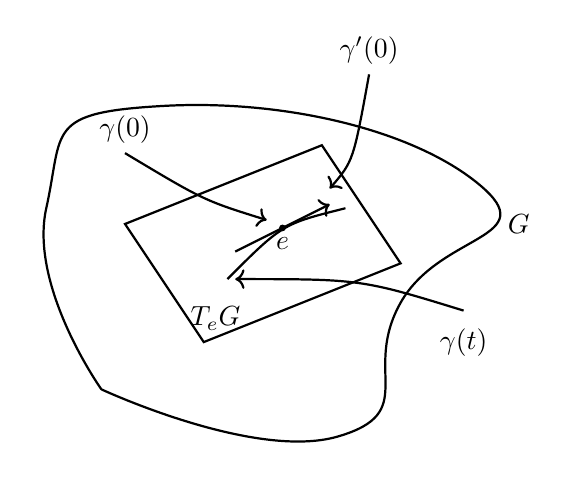
\begin{tikzpicture}
		
		% Draw the manifold G
		\draw[thick] plot [smooth,tension=1] 
		coordinates {(0.2,1.4) (3.2,0.8) (4,2.5) (5,4) (1,5) (-0.5,3.7) (0.2,1.4)};
		%\draw[thick] (0,0) to[out=30, in=180] (4,2.5) to[out=0, in=270] (5,4) to[out=90, in=30] (1,5) to[out=210, in=150] cycle;
		
		% Label G
		\node at (5.5,3.5) {$G$};
		
		% Draw the tangent space T_eG
		\draw[thick] (1.5, 2) -- (4, 3) -- (3, 4.5) -- (0.5, 3.5) -- cycle;
		
		% Label TeG
		\node at (1.65, 2.3) {$T_e G$};
		
		% Draw the curve \gamma(t)
		\draw[thick] (1.8, 2.8) .. controls (2.5, 3.5) .. (3.3, 3.7);
		
		% Label points and vectors
		\node at (0.5,4.7) {$\gamma(0)$};
		\draw[thick, ->] (0.5,4.4) .. controls (1.5,3.8) .. (2.3,3.55);
		\node at (4.8, 2) {$\gamma(t)$};
		\draw[thick, ->] (4.8,2.4) .. controls (3.5,2.8) .. (1.9,2.8);
		\filldraw[black] (2.5,3.45) circle (1pt) node[anchor=north] {$e$};
		\draw[thick, ->] (1.9, 3.15) -- (3.1, 3.75);
		\node at (3.6, 5.7) {$\gamma'(0)$};
		\draw[thick, ->] (3.6, 5.4) .. controls (3.4,4.3) .. (3.1,3.95);
		
	\end{tikzpicture}
\end{figure}
由解的形式可见,对于$G$在幺元处的切空间$T_eG$的任意一个向量$A=\gamma'(0)$,就有$G$中的一元素$\gamma(1)=\exp(\gamma'(0))$与之对应.现在我们稍微总结一下:对于李群$G$这个流形,我们可以找到其单参数子群$T_eG$作为其切空间,并且我们可以找到一个指数映射从切空间到原空间,很快,当我们学会李代数的时候,我们会再次使用李代数的语言来总结:``李代数就是李群的切空间所导出的代数".

我们再次回到群$G$和它的单参数子群,我们发现,如果给定$G$中与幺元邻近的一个元素\footnote{当然,由于我们研究线性群,幺元为单位矩阵.}$g$,并定义向量$A=\log g$,则由$e^A=g$ 知,$A$ 为$G$ 在$e$ 处之切向量,$e^tA$为以 $A$ 为单位切向量的单参数子群.因此,对$G$ 中与幺元$e$ 邻近的一个元素就有$T_{e}(G)$($G$ 在幺元处的切空间)中一向量$A$ 与之对应,也就是说,设$U\subset G$ 中包含$e$ 的一个适当邻域,我们建立了一种对应关系
\begin{equation}
	\begin{aligned}
		G\supset U&\overunderset{\log}{\exp}{\longleftrightarrow}T_{e}(G)\\g&\to A=\log g\\e^{A}&\leftarrow A
	\end{aligned}
\end{equation}
这种对应关系可以使我们对李群的研究转化到与其对应的在幺元$e$处的切空间$T_e(G)$.而我们知道,$T_e(G)$是由向量组成的线性空间,其线性结构具有先天优势,拥有远比李群简单的结构和运算.但由于我们前面所提到的,由于矩阵乘法相比于数乘的不可交互性,自然由此导出的切空间的运算自然也不能简单用普通加减法来表述,即如下关系
\begin{equation}
	\begin{aligned}&T_{e}(G)\qquad G\\&A\quad\longrightarrow\quad e^{A}\\&B\quad\longrightarrow\quad e^{B}\\&A+B\to e^{A+B}\ne e^{A}e^{B}\end{aligned}
\end{equation}
为此,我们迫切需要引入一种新的代数结构来反映$G$中的不可交换性,而具有这种新结构的线性空间$T_e(G)$
,就是我们下一节所要讲的\textbf{李代数}.
\section{李群与李代数}
\subsection{李代数}
由上面的讨论,我们现在知道$e^Ae^B\ne e^{A+B}$,那么,问题自然变为:$e^Ae^B=e^{?}$,或者表述为,$G$的单参数子群的代数结构是什么样的?

为了解决这个问题,我们设$A,B\in T_e(G)$,取一个参数$t$,并要求$|t|$适当小,从而能够保证$e^{tA}$与$e^{tB}$均为李群$G$中与幺元$e$邻近的元素\footnote{这个要求是必要的,我们需要满足后续使用级数的收敛性.}.现在我们构造一个函数:
\begin{equation}
	g(t)=e^{tA}e^{tB}e^{-tA}e^{-tB}
\end{equation}
显然,对于特例,即如果$e^{tA}$与$e^{tB}$可交换,$g(t)=e=\textbf{1}$,对于不可交换的情况,$g(t)$与幺元$e$的偏离程度反映了$e^{tA}$与$e^{tB}$的乘法与可交换的乘法之间的差异大小.现在我们具体分析$g(t)$.
\begin{equation}
	\begin{aligned}
		g(t)& =e^{tA}e^{tB}e^{-tA}e^{-tB} \\
		&=(\textbf{1}+tA+\frac{t^{2}}{2!}A^{2}+\frac{t^{3}}{3!}A^{3}+\cdots)(\textbf{1}+tB+\frac{t^{2}}{2!}B^{2}+\frac{t^{3}}{3!}B^{3}+\cdots) \\
		&(\textbf{1}-tA+\frac{t^2}{2!}A^2-\frac{t^3}{3!}A^3+\cdots)(\textbf{1}-tB+\frac{t^2}{2!}B^2-\frac{t^3}{3!}B^3+\cdots) \\
		&=\{\textbf{1}+t(A+B)+t^{2}(\frac{A^{2}}{2}+AB+\frac{B^{2}}{2})+t^{3}(\frac{A^{3}}{6}+\frac{A^{2}B}{2}+\frac{AB^{2}}{2}+\frac{B^{3}}{6})+O(t^{4})\} \\
		&\{\textbf{1}-t(A+B)+t^2(\frac{A^2}{2}+AB+\frac{B^2}{2})-t^3(\frac{A^3}{6}+\frac{A^2B}{2}+\frac{AB^2}{2}+\frac{B^3}{6})+O(t^4)\} \\
		&=\textbf{1}+t(A+B-A-B)+t^{2}(AB-BA)+t^{3}(\frac{A^{2}B}{2}-\frac{AB^{2}}{2}- \\
		&-\frac{B^2A}{2}+\frac{BA^2}{2}-ABA+BAB)+O(t^4) \\
		&=\textbf{1}+t^{2}[A,B]+\frac{t^{3}}{2}([A,[A,B]]-[B,[B,A]])+O(t^{4})
	\end{aligned}
\end{equation}
这里我们使用了对易子记号$[,]$,不过对于李代数,它也称为李括号,李乘法\footnote{事实上,对于线性群它等同于对易子,后面会加以区分的使用对易子和李括号.}.对于函数$g(t)$,我们有
\begin{equation}
	\frac{g(t)-\textbf{1}}{t^2}=[A,B]+O(t)
\end{equation}
因此,考虑极限$t\to0$时,
\begin{equation}
	\lim_{t\to0}\frac{g(t)-\textbf{1}}{t^{2}}=[A,B]
\end{equation}
由此,我们发现李群$G$的元素$e^{tA}$与$e^{tB}$的乘法的不可交换程度在$|t|$很小时主要取决于$[A,B]$

现在我们做变量代换$t=\sqrt{s}$,则
\begin{equation}
	\frac{g(\sqrt{s})-g(0)}{s}=[A,B]+O(\sqrt{s})
\end{equation}
并因此
\begin{equation}
	\lim_{s\to0}\frac{g(\sqrt{s})-g(0)}{s}=[A,B]
\end{equation}
这也说明$[A,B]$是李群$G$中过幺元的曲线$g(\sqrt{s})$在幺元处的\textbf{切向量},即$[A,B]\in T_e(G)$,这也意味着我们证明了如下关系
\begin{equation}
	\forall A,B\in T_{e}(G) , [A,B]\in T_{e}(G)
\end{equation}
即对易子(李括号)对向量空间$T_e(G)$的封闭性.


此时,我们可以回答开头所提到的问题了,不妨设$e^{tA}e^{tB}=e^{tC}$,则
\begin{equation}
	\begin{aligned}
		tC&=\log e^{tC}=\log e^{tA}e^{tB}\\
		&=\log\{(\textbf{1}+t(A+B)+\frac{t^{2}}{2}(A^{2}+2AB+B^{2})+ \\
		&\quad+\frac{t^{3}}{6}(A^{3}+3A^{2}B+3AB^{2}+B^{3})+O(t^{4})\} \\
		&=t(A+B)+\frac{t^{2}}{2}(A^{2}+2AB+B^{2})+\frac{t^{3}}{6}(A^{3}+3A^{2}B+3AB^{2}+B^{3})+O(t^{4}) \\
		&\quad-\{t(A+B)+\frac{t^2}{2}(A^2+2AB+B^2)+O(t^3)\}^2/2+ \\
		&\quad+\{t(A+B)+\frac{t^{2}}{2}(A^{2}+2AB+B^{2})+O(t^{3})\}^{3}/3+O(t^{4}) \\
		&=t(A+B)+\frac{t^{2}}{2}(AB-BA)+\frac{t^{3}}{12}(A^{2}B-ABA-ABA+BA^{2} \\
		&\quad-B^2A+BAB+BAB-AB^2)+O(t^4) \\
		&=(tA+tB)+\frac{1}{2}[tA,tB]+\frac{1}{12}[tA,[tA,tB]-tB,[tB,tA]]+O(t^{4}) 
	\end{aligned}
\end{equation}
由此可见,只要给出李括号,$T_e(G)$中知道了与$e^{tA},e^{tB}$相对应的元素$tA,tB$即可求得$T_e(G)$中与$e^{tA}e^{tB}$相对应的元素.因此,我们认为李括号可以表述李群切空间的代数结构,并对于李括号有下列性质(事实上完全类似在第一章给出过的对于对易子的同样性质).
\begin{equation}
	\begin{gathered}
		\left\lbrack {A, A}\right\rbrack = 0\\
		\left\lbrack {A, B}\right\rbrack = - \left\lbrack {B, A}\right\rbrack\\
		\left\lbrack {A, c}\right\rbrack = 0\;\left( {c\text{ 只是一个数 }}\right)\\
		\left\lbrack {A + B, C}\right\rbrack = \left\lbrack {A, C}\right\rbrack + \left\lbrack {B, C}\right\rbrack\\
		\left\lbrack {A,{BC}}\right\rbrack = \left\lbrack {A, B}\right\rbrack C + B\left\lbrack {A, C}\right\rbrack\\
		\left\lbrack {A,\left\lbrack {B, C}\right\rbrack }\right\rbrack + \left\lbrack {B,\left\lbrack {C, A}\right\rbrack }\right\rbrack + \left\lbrack {C,\left\lbrack {A, B}\right\rbrack }\right\rbrack = 0
	\end{gathered}
\end{equation}

我们称有了李括号的向量空间$T_e(G)$构成一个李代数,更准确的来讲是李群$G$的李代数,并记为$\mathfrak{g}$.\\
李群的李代数完全刻画了李群在幺元附近的结构,而要研究李群在幺元附近的性质只需要研究李代数即可,但是需要注意的是,李代数\textbf{仅}刻画了李群在幺元附近的\textbf{局部}性质,\textbf{不能}反映其整体性质,一个李群对应一个李代数,而一个李代数可以对应多个李群.
\subsection{李氏三定理}
1
\subsection{典型李群和李代数}
1
\section{李代数(Lie Algebra)}
\subsection{基,伴随算符,内积}
1
\subsection{正交补空间}
1
\subsection{李代数的结构}
1
\section{卡西米尔算符(Casimir operator)}
\section{张量}
\subsection{定义,分类,性质}
1
\subsection{不可约张量的分解}
1
\section{李群和李代数的表示及其约化}
	
\section{李代数应用的物理实例}
	
\ifx\allfiles\undefined
\end{document}
	\else
	\fi

\ifx\allfiles\undefined

% 如果有这一部分另外的package,在这里加上
% 没有的话不需要

\begin{document}
	\else
	\fi
\chapter{场论初步}
\begin{introduction}
	\item 路径积分
	\item 传播子
	\item 配分函数
	\item 系综
\end{introduction}
\begin{comment}
	注释:可爱且漂亮的公式形式.
	\begin{equation}
		\vspace{\baselineskip}
		
		定位点a \tikzmarknode{a}{\highlight{red颜色}{$公式内容$}}
		定位点s \tikzmarknode{s}{\highlight{blue}{$公式内容$}}
		
		定位点编码标准:1eq1 (公式序号eq该公式第几个)
	\end{equation}
	\begin{tikzpicture}[overlay,remember picture,>=stealth,nodes={align=left,inner ysep=1pt},<-]
	% 对于 "1" 定位点
	\path (1eq1.north) ++ (0,2em) node[anchor=south east,color=red!67] (eq1/1){\textbf{动能}};
	\draw [color=red!87](1eq1.north) |- ([xshift=-0.3ex,color=red]eq1/1.south west);
	% 对于 "2" 定位点
	\path (1eq2.south) ++ (0,-1.5em) node[anchor=north west,color=blue!67] (eq1/2){\textbf{势能}};
	\draw [color=blue!57](1eq2.south) |- ([xshift=-0.3ex,color=blue]eq1/2.south east);
	\end{tikzpicture}
\end{comment}
在这一章,我们正式进入主题,同时也是最重要的开始部分,在这一章我们会接触许多新概念,我将尽量的把内容详细的解释出来,在后续的时候可能会对其进行再编辑,请以最新版本为准!
\section{路径积分}
在初等量子力学的学习中,我们在经典量子化的框架内进行表述,在本节,我们将初步探索另一种表述方法:\textbf{路径积分法}.
\subsection{量子系统与经典系统中的路径积分}
我们采取通过一个最基本物理图像的方式来引入路径积分:考虑一维空间内的一个有质量$ m $的粒子,其动力学可以通过拉格朗日量来表述:\footnote{本章开始采取这类更加清晰的公式标注方法.}\\
	
\begin{equation}
	\vspace{\baselineskip}
	L(q,\dot{q})=\tikzmarknode{1eq1}{\highlight{red}{$\frac12m\dot{q}^2$}}-\tikzmarknode{1eq2}{\highlight{blue}{$V(q)$}}
\end{equation}
	\begin{tikzpicture}[overlay,remember picture,>=stealth,nodes={align=left,inner ysep=1pt},<-]
		% 对于 "1" 定位点
		\path (1eq1.north) ++ (0,2em) node[anchor=south east,color=red!67] (eq1/1){\textbf{动能项}};
		\draw [color=red!87](1eq1.north) |- ([xshift=-0.3ex,color=red]eq1/1.south west);
		% 对于 "2" 定位点
		\path (1eq2.south) ++ (0,-1.5em) node[anchor=north west,color=blue!67] (eq1/2){\textbf{势能项}};
		\draw [color=blue!57](1eq2.south) |- ([xshift=-0.3ex,color=blue]eq1/2.south east);
	\end{tikzpicture}
	
并假设粒子位于与时间无关的势$ V(q) $中.我们使用广义坐标$ q $来表述粒子的位置\footnote{广义坐标往往指一组无关联约束的坐标,即对于三维坐标表述,如果$x,y,z$之间没有约束方程,那么$x,y,z$就可以认为是一组广义坐标.不过,目前可以仅把它们当做特殊的坐标/动量(对于广义动量).},对于广义坐标,同样有$\dot{q}=\partial_t q$.于是,根据我们在理论力学中所学到的欧拉-拉格朗日方程
\begin{equation}
	\frac{\d}{\dt}\frac{\partial L(q,\dot{q})}{\partial\dot{q}}=\frac{\partial L(q,\dot{q})}{\partial q}\quad\text{也就是}\quad m\ddot{q}=-\frac{\partial V(q)}{\partial q}.
\end{equation}
同时,我们考虑由下式定义的\textbf{哈密顿量}$H(p,q)$
\begin{equation}
 H(p,q)=p\dot{q}-L(q,\dot{q})=\frac{p^2}{2m}+V(q)\quad\text{其中广义坐标被定义为}\quad p=\frac{\partial L(q,\dot{q})}{\partial\dot{q}}=m\dot{q}
\end{equation}
我们于是通过哈密顿量给出该粒子的经典动力学关系(特别强调的一点是,在对哈密顿量偏导时,我们认为广义坐标和广义动量是无关联的.):
\begin{equation}
	\dot{p}=-\frac{\partial H(p,q)}{\partial q}=-\frac{\partial V(q)}{\partial q},\dot{q}=\frac{\partial H(p,q)}{\partial p}=\frac{p}{m}
\end{equation}

在量子力学中,我们把广义坐标和广义动量的关系上升至对易关系(后续我们把广义坐标和广义动量简称为坐标和动量).
\begin{equation}
	[\hat{q},\hat{p}]=i\hbar
\end{equation}
同时经典变量$A(p,q)$同时上升为算符$\hat{A}\equiv A(\hat{p},\hat{q})$自然经典哈密顿量也变为量子哈密顿量方程.
\begin{equation}
	\hat{H}=\frac{\hat{p}^2}{2m}+V(\hat{q})
\end{equation}


我们知道系统的物理态由希尔伯特空间$ \mathcal H $中的态矢量$|\psi(t)\ra$所描述,我们使用薛定谔方程来描述态矢量的时间演化:\\

\begin{equation}
	\vspace{\baselineskip}
	%公式编号: 7
	\tikzmarknode{7eq1}{\highlight{red}{$i\hbar\partial_t$}}|\psi(t)\rangle=\tikzmarknode{7eq2}{\highlight{blue}{$\hat{H}$}}|\psi(t)\rangle
\end{equation}
\begin{tikzpicture}[overlay,remember picture,>=stealth,nodes={align=left,inner ysep=1pt},<-]
	% 对于 "1" 定位点
	\path (7eq1.north) ++ (0,2em) node[anchor=south east,color=red!67] (eq7/1){\textbf{能量$ E $}};
	\draw [color=red!87](7eq1.north) |- ([xshift=-0.3ex,color=red]eq7/1.south west);
	% 对于 "2" 定位点
	\path (7eq2.south) ++ (0,-1.5em) node[anchor=north west,color=blue!67] (eq7/2){\textbf{哈密顿量算符}};
	\draw [color=blue!57](7eq2.south) |- ([xshift=-0.3ex,color=blue]eq7/2.south east);
\end{tikzpicture}

我们熟知我们可以利用时间演化算符$\hat U$写成方程的解:
\begin{equation}
	|\psi(t)\rangle=\hat{U}(t)|\psi(t=0)\rangle,\quad i\hbar\partial_t\hat{U}(t)=\hat{H}\hat{U}(t).
\end{equation}
由于哈密顿量与时间无关,所以我们可以写成时间演化算符的表示
\begin{equation}
	\hat{U}(t)=e^{-\frac i\hbar\hat{H}t}
\end{equation}
同时我们写出\\

\begin{equation}
	\vspace{\baselineskip}
	%公式编号: 10
	\tikzmarknode{10eq1}{\highlight{red}{$\psi(q_f,t_f)$}}=\langle q_f|\psi(t_f)\rangle=\langle q_f|\hat{U}(t_f-t_i)|\psi(t_i)\rangle=\int \dq_iU(q_f,q_i;t_f-t_i)\tikzmarknode{10eq2}{\highlight{blue}{$\psi(q_i,t_i)$}}
\end{equation}
\begin{tikzpicture}[overlay,remember picture,>=stealth,nodes={align=left,inner ysep=1pt},<-]
	% 对于 "1" 定位点
	\path (10eq1.north) ++ (0,2em) node[anchor=south west,color=red!67] (eq10/1){\textbf{$ t_f $时刻时粒子位于$q_f$的概率}};
	\draw [color=red!87](10eq1.north) |- ([xshift=-0.3ex,color=red]eq10/1.south east);
	% 对于 "2" 定位点
	\path (10eq2.south) ++ (0,-1.5em) node[anchor=north east,color=blue!67] (eq10/2){\textbf{$ t_i $时刻时粒子位于$q_i$的概率}};
	\draw [color=blue!57](10eq2.south) |- ([xshift=-0.3ex,color=blue]eq10/2.south west);
\end{tikzpicture}

其中$U(q_f,q_i;t_f-t_i) = \langle q_f|\hat{U}(t_f-t_i)|q_i\rangle $被称为传播子,其表示了这个粒子在$t_f-t_i$时间内从位置$q_i$传播到位置$q_f$的概率振幅.并且若已知哈密顿量$\hat{H}$本征态$\{|n\ra,\epsilon_n\}$,那么我们以此可以把传播子写作
\begin{equation}
	\begin{aligned}U(q_f,q_i;t_f-t_i)&=\langle q_f|e^{-\frac{i}{\hbar}\hat{H}(t_f-t_i)}|q_i\rangle=\sum_n\langle q_f|n\rangle e^{-\frac{i}{\hbar}\epsilon_n(t_f-t_i)}\langle n|q_i\rangle\\[2ex]&=\sum_ne^{-\frac{i}{\hbar}\epsilon_n(t_f-t_i)}\varphi_n(q_f)\varphi_n^*(q_i)\end{aligned}
\end{equation}
其中$\varphi_n(q)=\la q|n\ra$为坐标表象下的波函数.我们发现传播子给出了关于这个哈密顿量的波函数和能级的全部信息,这也意味着我们可以把求解波函数的问题变为求解这个哈密顿量所对应的传播子的问题.
\subsection*{路径积分}
我们刚刚发现了通过求解传播子可以间接求解波函数,而现在的问题是:如何求出传播子? 这里我们用到费曼的路径积分方法,我们先来首先说明\textbf{传播子可以写为路径积分的形式}.

我们首先考虑一个充分短的时间$\epsilon$

\begin{equation}
	\vspace{\baselineskip}
	%公式编号: 12
	U(q_f,q_i;\epsilon)=\langle q_f|e^{-i\hat{H}\epsilon}|q_i\rangle \tikzmarknode{12eq2}{\highlight{blue}{$\simeq$}}\langle q_f|e^{-i\epsilon\frac{\hat{p}^2}{2m}}e^{-i\epsilon V(\hat{q})}|q_i\rangle
\end{equation}
\begin{tikzpicture}[overlay,remember picture,>=stealth,nodes={align=left,inner ysep=1pt},<-]
	% 对于 "2" 定位点
	\path (12eq2.south) ++ (0,-1.5em) node[anchor=north east,color=blue!67] (eq12/2){\textbf{Baker–Hausdorff规则$e^{\epsilon\hat{A}+\epsilon\hat{B}}=e^{\epsilon\hat{A}}e^{\epsilon\hat{B}}e^{\mathcal{O}(\epsilon^{2})}$}};
	\draw [color=blue!57](12eq2.south) |- ([xshift=-0.3ex,color=blue]eq12/2.south west);
\end{tikzpicture}

我们在其中插入一个单位算符的谱分解\footnote{此时已经开始采取自然单位制了(对单位制可以参考附录).},在下面的式子中,我们使用了归一化假设$\la q|p\ra=L^{-1/2}e^{ipq}\;q\in[0,L]$,$ q $为连续的位置变量,而$p=n\frac{2\pi}L\;n\in \mathbb Z$为离散的动量变量(关于边界$ L $,并且有归一化条件$e^{ipL}=1$),在极限$L\to\infty$,存在$\frac1L\sum_p\to\int_{-\infty}^\infty\frac{\d p}{2\pi}$.\\
于是,式子变为
\begin{equation}
	\vspace{\baselineskip}
	%公式编号: 13
	\begin{aligned}
		U(q_f,q_i;\epsilon)& \begin{aligned}&=\sum_p\langle q_f|e^{-i\epsilon\frac{\hat{p}^2}{2m}}|p\rangle\langle p|e^{-i\epsilon V(\hat{q})}|q_i\rangle\end{aligned} \\
		&=\int\frac{\d p}{2\pi}\exp\biggl\{-i\epsilon\biggl[\frac{p^2}{2m}+V(q_i)\biggr]+ip(q_f-q_i)\biggr\} \\
		&\tikzmarknode{13eq2}{\highlight{blue}{$=$}}\bigg(\frac{m}{2\pi i\epsilon}\bigg)^{1/2}\exp\bigg\{i\epsilon\bigg[\frac{m}{2}\frac{(q_{f}-q_{i})^{2}}{\epsilon^{2}}-V(q_{i})\bigg]\bigg\}.
	\end{aligned}
\end{equation}
\begin{tikzpicture}[overlay,remember picture,>=stealth,nodes={align=left,inner ysep=1pt},<-]
	% 对于 "2" 定位点
	\path (13eq2.south) ++ (0,-1.5em) node[anchor=north west,color=blue!67] (eq13/2){\textbf{此处计算需要利用留数定理,附录中给出了mma计算代码}};
	\draw [color=blue!57](13eq2.south) |- ([xshift=-0.3ex,color=blue]eq13/2.south east);
\end{tikzpicture}

为了使对$ p $的积分收敛,我们假设$\epsilon$包含一个小的负虚部,我们发现,指数上的部分恰好是$ i $乘以无穷小作用量$S(q_f,q_i;\epsilon)$,不难发现这个作用量对应着无穷小时间$\epsilon$内$ q_i $和$ q_f $之间以恒定速度的直线路径,于是,我们把式子写为如下形式:
\begin{equation}\label{4eq14}
	U(q_f,q_i;\epsilon)=\left(\frac{m}{2\pi i\epsilon}\right)^{1/2}e^{iS(q_f,q_i;\epsilon)+\mathcal{O}(\epsilon^2)}
\end{equation}
仅有无穷小时间间隔的传播子显然是远远不够的,现在我们想计算出任意时间间隔$t_f-t_i$的传播子$U(q_f,q_i;t_f-t_i)$.我们考虑将时间段$t_f-t_i$分割为$ N $个长为$\epsilon=(t_f-t_i)/N$的等大小的部分,只要最终我们取极限$N\to\infty\;(\epsilon\to0)$,并对全部时间步积分,就得到了任意时间间隔$t_f-t_i$的传播子.
\begin{equation}
	\begin{aligned}
		\begin{aligned}U(q_f,q_i;t_f-t_i)\end{aligned}& \begin{aligned}=\langle q_{f}|e^{-i\hat{H}\epsilon}\cdots e^{-i\hat{H}\epsilon}|q_{i}\rangle\end{aligned} \\
		&=\int\prod_{k=1}^{N-1}\d q_k\langle q_f|e^{-i\hat{H}\epsilon}|q_{N-1}\rangle\langle q_{N-1}|e^{-i\hat{H}\epsilon}|q_{N-2}\rangle\cdots\langle q_1|e^{-i\hat{H}\epsilon}|q_i\rangle \\
		&=\int\prod_{k=1}^{N-1}\d q_k\prod_{k=1}^NU(q_k,q_{k-1};\epsilon)
	\end{aligned}
\end{equation}
其中$q_0=q_i,q_N=q_f$,在\ref{4eq14}中,我们对每个时间步传播子都忽略了$\epsilon^2$的高阶项,对于整体,其导致了阶为$\epsilon$的总误差. \\
现在我们继续考虑,令$N\to\infty$我们有
\begin{equation}
	U(q_f,q_i;t)=\lim_{N\to\infty}\left(\frac{mN}{2\pi it}\right)^{N/2}\int\prod_{k=1}^{N-1}\d q_k e^{iS[q]}
\end{equation}
其中作用量为
\begin{equation}
	S[q]=\sum_{k=1}^NS(q_k,q_{k-1};\epsilon)=\epsilon\sum_{k=1}^N\left[\frac m2\frac{(q_k-q_{k-1})^2}{\epsilon^2}-V(q_{k-1})\right]
\end{equation}
在极限$N\to\infty$,我们可以把求和写做积分:
\begin{equation}
	\begin{aligned}\epsilon\sum_{k=1}^N\frac{m}{2}\frac{(q_k-q_{k-1})^2}{\epsilon^2}&\to\int_{t_i}^{t_f} \d t\frac{m}{2}\dot{q}^2\\\epsilon\sum_{k=1}^NV(q_{k-1})&\to\int_{t_i}^{t_f} \d t V(q)\end{aligned}
\end{equation}
我们使用$q(t)$表示这个粒子的``路径"(trajectory),对于始末位置$q(t_i)=q_i,q(t_f)=q_f$,但这并不意味着在大$ N $极限下的连续性/可微性.我们定义积分测度为如下形式\footnote{我们可以认为这个形式不过是把一些成套的东西包装成一个微分算符,依赖这种写法,可以简化我们对于路径积分的表述.}:
\begin{equation}
	\mathcal{D}[q]=\lim_{N\to\infty}\left(\frac{mN}{2\pi i\hbar t}\right)^{N/2}\prod_{k=1}^{N-1}\d q_k
\end{equation}
于是传播子可以简化为
\begin{equation}
	U(q_f,q_i;t_f-t_i)=\int_{q(t_i)=q_i}^{q(t_f)=q_f}\mathcal{D}[q]e^{\frac{i}{\hbar}S[q]}
\end{equation}
同时作用量被定义为

\begin{equation}
	\vspace{\baselineskip}
	%公式编号: 21
	\tikzmarknode{21eq1}{\highlight{red}{$S[q]$}}=\int_{t_i}^{t_f}\d t\tikzmarknode{21eq2}{\highlight{blue}{$L(q,\dot{q})$}}
\end{equation}
\begin{tikzpicture}[overlay,remember picture,>=stealth,nodes={align=left,inner ysep=1pt},<-]
	% 对于 "1" 定位点
	\path (21eq1.north) ++ (0,2em) node[anchor=south east,color=red!67] (eq21/1){\textbf{作用量}};
	\draw [color=red!87](21eq1.north) |- ([xshift=-0.3ex,color=red]eq21/1.south west);
	% 对于 "2" 定位点
	\path (21eq2.south) ++ (0,-1.5em) node[anchor=north west,color=blue!67] (eq21/2){\textbf{拉格朗日量}};
	\draw [color=blue!57](21eq2.south) |- ([xshift=-0.3ex,color=blue]eq21/2.south east);
\end{tikzpicture}

现在我们发现,这个作用量的形式与路径$q(t)$的经典作用量的形式一致.

我们不难注意到:积分测度$\mathcal D$中包含的极限是\textbf{发散的},在处理发散问题之前,我们首先尝试讨论其物理含义:对于传播子,我们从公式角度出发观察传播子的形式,我们不难发现这个积分过程只规定了初值条件(初态位置和时间以及末态位置和时间),我们需要对\textbf{所有可能的}路径进行积分(或者说是求和,这两者并没有太大区别),并且对于求和过程,我们最后得出的答案是依赖于作用量的对每条路径的\textbf{加权和}.而按照物理情景的解释,我们有``当一个物理过程\footnote{我们并没有区别宏观和微观,这是因为其对宏观仍然适用,但由于对应原理,我们不必对宏观现象如此分析.}可以以多种路径进行时,它的概率幅由每种路径的幅值之和给出\footnote{英文原文:When a
	process can take place in more than one way, its probability amplitude is given by the
	sum of the amplitudes for each way.}".

但是,我们发现这并没有解决发散问题,于是我们要求路径是足够``好"的.即要求动力学项$[q(t+\epsilon)-q(t)]^2/\epsilon$在极限$\epsilon\to0$时收敛,并认为在不满足这个条件的路径会剧烈震荡,其平均值为$ 0 $,即不那么``好"的路径.事实上,这种方法似乎完全看不出来严格的数学依据,但现实如此(这里可以引用那些经典的物理小笑话了,至少我们目前不用去思考如何把这些东西严谨化.)\footnote{关于这一大段的文字讨论是必须的,其有助于构建量子场论的物理图景,事实上,在这一章我一直在尝试把更多重点放在公式内部并突出显示它,倘若把重点置于一大堆文字中,读者不加以仔细的阅读的话,便很容易错过去.而且,对于物理这一门学科,过于长段的文字很难真的揭示什么内涵,它们往往起到解释公式的作用,或者说,公式才是文章的主体.同样的,这一大段内容我放在了脚注中,同样为了让人们去注意到它.}.

\subsection*{经典极限}
或许你们发现在上一部分的结尾中,我们并没有像往常一样去省略约化普朗克常数$\hbar$,这有关于经典极限的讨论.

我们所关注的重点路径为``贴近"经典路径的路径,其作用量是静态的.
\begin{equation}
	\left.\frac{\delta S[q]}{\delta q(t)}\right|_{q=q_c}=0
\end{equation}
对于非静态的路径,其意味着作用量的大幅振荡,其平均值为0,或者说,更准确的,传播子$U(q_f,q_i;t_f-t_i)$由路径$q(t)$所主导,其作用量$S[q]$与经典作用量$S_c=S[q_c]$相差一个$\hbar$阶项:$|S-S_c|\lesssim\hbar$.当$|S_c|\gg\hbar $时,这些路径非常接近经典作用量的路径.而对于相反的极限中,同样满足条件$|S-S_c|\lesssim\hbar$的路径就与经典作用量导致的路径截然不同.于是,形式上的经典极限对于与$\hbar\to0$的极限.

\begin{remark}
		\textit{为了得到极限$\hbar\to0$中的传播子,我们写出$q(t)=q_c(t)+r(t)$(我们假设仅存在唯一一条经典轨道.),并把作用量对于$r(t)$展开到第二阶.}
		\begin{equation}
			\begin{aligned}&U(q_f,q_i;t_f-t_i)\\&\simeq e^{\frac{i}{\hbar}S[q_c]}\int_{r(t_i)=0}^{r(t_f)=0}\mathcal{D}[r]\exp\biggl\{\frac{i}{2\hbar}\int_{t_i}^{t_f}\d t \d t' \frac{\delta^2S[q]}{\delta q(t)\delta q(t')}\biggr|_{q=q_c}r(t)r(t')\biggr\}\end{aligned}
		\end{equation}
		\textit{这类积分被称为\textbf{高斯积分},高斯积分并不需要你去思考如何巧妙积分出来,仅需套用公式就能得出答案,而对应的积分表全部列在下面,即式\ref{GaussIntegral}.}
		\begin{equation}
			U(q_f,q_i;t_f-t_i)\simeq e^{\frac{i}{\hbar}S[q_c]}\det\left(\frac{1}{2\pi i\hbar}\frac{\delta^2S[q]}{\delta q(t)\delta q(t')}\bigg|_{q=q_c}\right)^{-1/2}
		\end{equation}
		\textit{我们最后得到的结果所遵循的过程被称为稳态相位近似.}
\end{remark}
\subsection*{高斯积分表}
如下表,其中$ K $是对称矩阵.
\begin{equation}\label{GaussIntegral}
	\begin{alignat}{2}
		&\int_{-\infty}^{+\infty} e^{-\frac{1}{2}ax^{2}}\dx=\sqrt{\frac{2\pi}{a}} &\quad
		&\int_{-\infty}^{+\infty}x^{2n}e^{-\frac12ax^2}\dx=\sqrt{2\pi}a^{-\frac{2n+1}2}(2n-1)!! \\
		&\int_{-\infty}^{+\infty}e^{-\frac12ax^2+Jx}\dx=\sqrt{\frac{2\pi}a}e^{\frac{J^2}{2a}} &
		&\int_{-\infty}^{+\infty} e^{-\frac{1}{2} ax^{2}+iJx} \dx=\sqrt{\frac{2\pi}{a}}e^{-\frac{J^{2}}{2a}} \\
		&\int_{-\infty}^{+\infty}e^{i(\frac{1}{2}ax^{2}+Jx)}\dx=\sqrt{\frac{2\pi i}{a}}e^{-i\frac{J^{2}}{2a}} &
		&\int_{-\infty}^{+\infty}e^{-\frac{1}{2}x^{T}Kx}\d^{n}x=\sqrt{\frac{(2\pi)^{n}}{\det K}} \\
		&\int_{-\infty}^{+\infty}e^{-\frac{1}{2}x^{T}Kx+Jx}\d^{n}x=\sqrt{\frac{(2\pi)^{n}}{\det K}}e^{\frac{1}{2}JK^{-1}J} &
		&\int_{-\infty}^{+\infty}e^{-\frac{1}{2}x^{T}Kx+iJx}\d^{n}x=\sqrt{\frac{(2\pi)^{n}}{\det K}}e^{-\frac{1}{2}JK^{-1}J} \\
		&\int_{-\infty}^{+\infty}e^{i(\frac{1}{2}x^{T}Kx+Jx)}\d^{n}x=\sqrt{\frac{(2\pi i)^{n}}{\det K}}e^{-\frac{i}{2}JK^{-1}J}
	\end{alignat}
\end{equation}
需要强调的是,虽然看似高斯积分较为复杂,但都处于高等数学范畴内的积分,如需要记忆的话也可以仅记忆下面这个,其他都可以通过简单的系数替换得到:
\begin{equation}
	\int_{-\infty}^{+\infty}e^{-\frac12ax^2+Jx}\dx=\sqrt{\frac{2\pi}a}e^{\frac{J^2}{2a}}
\end{equation}
\subsection*{时序算符以及哈密顿量}
对于海森堡绘景下算符的矩阵元,例如算符$\hat{q}(t)=e^{i\hat{H}t}\hat{q}e^{-i\hat{H}t}$
\begin{equation}
	\langle q_f,t_f|\hat{q}(t)|q_i,t_i\rangle=\langle q_f|e^{-i\hat{H}(t_f-t)}\hat{q}e^{-i\hat{H}(t-t_i)}|q_i\rangle 
\end{equation}
如之前那样,我们将时间间隔无限拆分并再次积分,就可以得到矩阵元的路径积分表示:
\begin{equation}
	\langle q_f,t_f|\hat{q}(t)|q_i,t_i\rangle=\int_{q(t_i)=q_i}^{q(t_f)=q_f}\mathcal{D}[q] q(t)e^{iS[q]}
\end{equation}
而为了使用路径积分表示两个不同时间的算符的乘积,我们引入一个新算符,其被定义为\\

\begin{equation}
	\vspace{\baselineskip}
	%公式编号: 29
	\tikzmarknode{29eq1}{\highlight{red}{$T$}}\left[\prod_{i=1}^n\hat{q}_i(t_i)\right]=\sum_p\left(\prod_{j=1}^{n-1}\tikzmarknode{29eq2}{\highlight{blue}{$\Theta(t_{p_j}-t_{p_{j+1}})$}}\right)\epsilon\prod_{k=1}^{n}\hat{q}_{pk}(t_{pk})
\end{equation}
\begin{tikzpicture}[overlay,remember picture,>=stealth,nodes={align=left,inner ysep=1pt},<-]
	% 对于 "1" 定位点
	\path (29eq1.north) ++ (0,2em) node[anchor=south east,color=red!67] (eq29/1){\textbf{时序算符}};
	\draw [color=red!87](29eq1.north) |- ([xshift=-0.3ex,color=red]eq29/1.south west);
	% 对于 "2" 定位点
	\path (29eq2.south) ++ (0,-1.5em) node[anchor=north west,color=blue!67] (eq29/2){\textbf{阶跃函数,即$x\ge0\to\Theta(x)=1;x<0\to\Theta(x)=0$}};
	\draw [color=blue!57](29eq2.south) |- ([xshift=-0.3ex,color=blue]eq29/2.south east);
\end{tikzpicture}

于是我们不难看出,虽然这个算符形式看起来十分复杂,但并没有对原来的算符进行实质性改变,只不过是按照时间顺序把这些算符的乘积进行排序,这也是这个算符被称为\textbf{时序算符}的原因.并且对于式子中的$\epsilon$,其对于玻色子算符总是取$+1$,对于费米子算符,其依赖于前面的排序的奇偶性:对于偶置换取正,对于奇置换取负.\\
我们以最简单的二阶情景为例:
\begin{equation}
	T\hat{q}(t)\hat{q}(t')=\Theta(t-t')\hat{q}(t)\hat{q}(t')+\Theta(t'-t)\hat{q}(t')\hat{q}(t)
\end{equation}
其路径积分表示为
\begin{equation}
	\langle q_f,t_f|T\hat{q}(t)\hat{q}(t')|q_i,t_i\rangle=\int_{q(t_i)=q_i}^{q(t_f)=q_f}\mathcal{D}[q] q(t)q(t')e^{iS[q]}
\end{equation}
回想这一形式的物理意义,我们发现路径积分自然表示了算符按一个时序的乘积的期望.

\subsection*{路径积分的哈密顿形式}
我们先前的作用量都是有拉格朗日形式给出,现在我们一并写出同样对于哈密顿形式的传播子,积分测度以及作用量:
\begin{equation}
	\begin{aligned}
		U(q_f,q_i;t_f-t_i)&=\lim_{N\to\infty}\int\prod_{k=1}^{N-1}\d q_{k}\int\prod_{k=1}^{N}\frac{\d p_{k}}{2\pi}e^{\sum_{k=1}^{N}\left[ip_{k}(q_{k}-q_{k-1})-i\epsilon\frac{p_{k}^{2}}{2m}-i\epsilon V(q_{k-1})\right]}\\
		&\equiv\int_{q(t_i)=q_i}^{q(t_f)=q_f}\mathcal{D}[p,q] e^{iS[p,q]} \\
		\mathcal{D}[p,q]&=\lim_{N\to\infty}\prod_{k=1}^{N-1}\d q_k\prod_{k=1}^N\frac{\d p_k}{2\pi}\\
		S[p,q]&=\lim_{N\to\infty}\sum_{k=1}^N\Big[p_k(q_k-q_{k-1})-\epsilon\frac{p_k^2}{2m}-\epsilon V(q_{k-1})\Big] \\
		&\equiv\int_{t_i}^{t_f}\dt [p\dot{q}-H(p,q)]
	\end{aligned}
\end{equation}








\subsection{欧式路径积分}
回忆我们在统计力学中的学习,通过配分函数可以得到几乎全部我们所关心的物理量,而同样的,对于凝聚态场论,我们仍需要重点关注配分函数.\\
我们首先写出配分函数的形式
\begin{equation}
	Z=\operatorname{Tr}e^{{-\beta\hat{H}}}=\int \d q\langle q|e^{{-\beta\hat{H}}}|q\rangle
\end{equation}
为了揭示经典与量子统计力学直接的联系,我们从演化算符$e^{-i\hat{H}t}$在一个虚时(时间为虚数)的情况下求解,其中虚时$t=-i\beta$(对于SI单位制,$t=-i\beta\hbar$),自然得出凝聚态场论中的配分函数.我们自然看出来一个重要的事情:经典统计力学与凝聚态场论(也称为量子统计力学)之间仅仅差了一个变换$t\to-i\tau$.我们称这个变换为\textbf{Wick转动(Wick rotation)}.即在复时间平面上旋转了$-\pi/2$角.虚时的概念在凝聚态场论中至关重要,我们依次作Wick转动,传播子变为:
\begin{equation}
	\begin{aligned}
		U(q_f,q_i;-i\tau)& \begin{aligned}&=\lim_{N\to\infty}\left(\frac{mN}{2\pi\tau}\right)^{N/2}\int\prod_{k=1}^{N-1}dq_k e^{-\epsilon\sum_{k=1}^N\left[\frac{m}{2}\frac{\left(q_k-q_{k-1}\right)^2}{\epsilon^2}+V\left(q_{k-1}\right)\right]}\end{aligned} \\
		&=\int_{q(0)=q_i}^{q(\tau)=q_f}\mathcal{D}[q] e^{-S_E[q]}.
	\end{aligned}
\end{equation}
对于虚时路径积分,同样的边界满足$q(0)=q_i;q(\tau)=q_f$,对于不同路径的权重同样有作用量给出:\\

\begin{equation}
	\vspace{\baselineskip}
	%公式编号: 35
	\tikzmarknode{35eq1}{\highlight{red}{$S_E[q]$}}=\int_{0}^{\tau}\d\tau'\tikzmarknode{35eq2}{\highlight{blue}{$\left[\frac m2\dot{q}^2+V[q]\right]$}}
\end{equation}
\begin{tikzpicture}[overlay,remember picture,>=stealth,nodes={align=left,inner ysep=1pt},<-]
	% 对于 "1" 定位点
	\path (35eq1.north) ++ (0,2em) node[anchor=south east,color=red!67] (eq35/1){\textbf{欧几里得作用量(欧式作用量)}};
	\draw [color=red!87](35eq1.north) |- ([xshift=-0.3ex,color=red]eq35/1.south west);
	% 对于 "2" 定位点
	\path (35eq2.south) ++ (0,-1.5em) node[anchor=north west,color=blue!67] (eq35/2){\textbf{欧式拉格朗日量(动能和势能同号)}};
	\draw [color=blue!57](35eq2.south) |- ([xshift=-0.3ex,color=blue]eq35/2.south east);
\end{tikzpicture}

经典极限对于虚时路径积分也是同样的,并且通过Wick旋转,我们可以将欧式作用量变为实时作用量:
\begin{equation}
	S_E[q]\xrightarrow[\tau=it]{\text{\textit{Wick 旋转}}}i\int_0^t\d t'\left[-\frac{m}{2}\dot{q}^2+V(q)\right]=-iS[q].
\end{equation}
自然可以继续写出配分函数为
\begin{equation}
	Z=\int \d qU(q,q,-i\beta)=\int_{q(\beta)=q(0)}\mathcal{D}[q]e^{{-S_{E}[q]}}
\end{equation}
作为所有周期为$\beta$的周期性路径的虚时路径积分,虚时算符$\hat{q}(\tau)=e^{\tau\hat{H}}\hat{q}e^{-\tau\hat{H}}$的期望自然写出
\begin{equation}
	\langle\hat{q}(\tau)\rangle=\frac{1}{Z}\mathrm{Tr}{\left[e^{-\beta\hat{H}}\hat{q}(\tau)\right]}=\frac{1}{Z}\int_{q(\beta)=q(0)}\mathcal{D}[q]q(\tau)e^{{-S_{E}[q]}}
\end{equation}
同样的,对于多个不同时间算符的时序乘积,我们利用时序算符按$\tau$进行排序,并有
\begin{equation}
	\langle T_\tau\hat{q}(\tau)\hat{q}(\tau^{\prime})\rangle=\frac1Z\int_{q(\beta)=q(0)}\mathcal{D}[q] q(\tau)q(\tau^{\prime})e^{-S_E[q]}
\end{equation}
如果$\beta\to0$或$\hbar\to0$,传播子$U(q,q;-i\beta\hbar)$就可以仅利用一个时间步($ N=1 $)计算出来\footnote{为了直观的和德布罗意关系联系起来,此处再次把$\hbar$显现出来}.其导致
\begin{equation}
	\begin{aligned}
		Z_{\mathrm{cl}}& \begin{aligned}&=\frac{1}{\hbar}\sqrt{\frac{m}{2\pi\beta}}\int \dq e^{-\beta V(q)}\end{aligned} \\
		&\equiv\int_{-\infty}^{\infty}\frac{\d p}{2\pi\hbar}\int_{-\infty}^{\infty}\dq \mathrm{exp}\bigg\{-\beta\bigg[\frac{p^{2}}{2m}+V(q)\bigg]\bigg\}
	\end{aligned}
\end{equation}
我们发现配分函数变为经典配分函数,在有限温度$T<\infty$的情况下,如果势能$V(q)$在德布罗意波长$\xi_{th}\sim\hbar/\sqrt{mT}$的数量级下的长度尺度缓慢变化,那么我们认为量子统计力学的配分函数退化为经典统计力学的配分函数,即\textbf{对应原理}.

方程还显示了经典系统的一个非常重要的特性:热力学和动力学是分离的:粒子的位置和动量是独立变量,可以积分出动量(这会产生对自由能的附加贡献作用),并仅以位置变量的形式写出配分函数.相比之下,在量子系统中,坐标和动量是两个不对易算符,因此静力学和动力学不是独立的.这就是为什么配分函数可以与虚时中的演化算子相关联的原因.

\begin{eggg}
	
	{\Large 已知空间内存在一个有质量的一维谐振子,质量为$ m $,频率为$\omega$.}\\
	我们首先考虑自由粒子时的简化情况(即$\omega\to0$)
\end{eggg}






































































































	
\ifx\allfiles\undefined
\end{document}
	\else
	\fi

\ifx\allfiles\undefined

% 如果有这一部分另外的package,在这里加上
% 没有的话不需要

\begin{document}
	\else
	\fi
\chapter{对称关系}
\begin{introduction}
	\item 诺特定理
	\item 简并
	\item 离散对称性
	\item 宇称
\end{introduction}
\section{简并}
\subsection{简并}
现在转向简并概念, 尽管简并可以在经典力学层次讨论一一例如, 在讨论开普勒问题中的闭合(非进动)轨道时(Goldstein 2002)——这个概念在量子力学中起着更重要的作用. 假设对某种对称性算符

$$
\left\lbrack {H,8}\right\rbrack = 0 tag{4.1.13}
$$

而 $|n\rangle$ 为能量本征右矢,本征值为 ${E}_{n}$ . 则 $g \mid n\rangle$ 也是一个具有相同能量的能量本征右矢, 因为

$$
H\left( {\delta |n\rangle }\right) = {\delta H}|n\rangle = {E}_{n}\left( {\delta |n\rangle }\right) . tag{4.1.14}
$$

假定 $\left| {n\rangle \text{和}g}\right| n\rangle$ 代表不同的态. 那么,它们就是具有相同能量的两个态一一这就是说, 它们是简并态. 通常, $8$ 由一个连续参量,比如 $\lambda$ ,表征,在这种情况下,所有的形式为 $g\left( \lambda \right) |n\rangle$ 的态都有相同的能量.

下面特别来考虑转动. 假定哈密顿量是转动不变的, 因此

$$
\left\lbrack {\mathcal{D}\left( R\right), H}\right\rbrack = 0, tag{4.1.15}
$$

它一定意味着

$$
\left\lbrack {\mathbf{J}, H}\right\rbrack = 0,\;\left\lbrack {{\mathbf{J}}^{2}, H}\right\rbrack = 0. tag{4.1.16}
$$

可以构成 $H,{\mathbf{J}}^{2}$ 和 ${J}_{z}$ 的共同本征态,用 $|n;j, m\rangle$ 表示. 刚刚给出的论据意味着所有下列形式的态

$$
\mathcal{D}\left( R\right) |n;j, m\rangle tag{4.1.17}
$$

具有相同的能量. 在第 3 章曾看到转动下不同的 $m$ 值要混起来. 一般而言, $\mathcal{D}\left( R\right) \mid n;j$ , $m\rangle$ 是 ${2j} + 1$ 个独立的态的线性组合. 显然,

$$
\mathcal{D}\left( R\right) \left| {n;j, m\rangle = \mathop{\sum }\limits_{{m}^{\prime }}}\right| n;j,{m}^{\prime }\rangle {\mathcal{D}}_{{m}^{\prime }m}^{\left( j\right) }\left( R\right) , tag{4.1.18}
$$

并且,通过改变表征转动算符 $\mathcal{D}\left( R\right)$ 的连续参量,可以得到 $\left| {n;j,{m}^{\prime }}\right\rangle$ 的不同的线性组合. 如果在任意的 $\mathcal{D}\left( R\right)$ 情况下,所有形为 $\mathcal{D}\left( R\right) \mid n;j, m\rangle$ 的态都有相同的能量,那时十分自然地,有着不同 $m$ 的 $|n;j, m\rangle$ 中,每一个都一定有相同的能量. 所以,在这里简并是 $\left( {{2j} + 1}\right)$ 重的,正好等于可能的 $m$ 值的个数. 从这样的事实来看这一点也是显然的. 即通过与 $H$ 对易的 ${J}_{ \pm }$ 相继作用于 $|n;{jm}\rangle$ 得到的所有的态,具有相同的能量.

作为一个应用,考虑一个原子中的电子,它所受到的势可以写成 $V\left( r\right) + {V}_{LS}\left( r\right) \mathbf{L} \cdot \mathbf{S}$ . 因为 $r$ 和 $\mathbf{L} \cdot \mathbf{S}$ 都是转动不变的,预期每一个原子能级都是 $\left( {{2j} + 1}\right)$ 重简并. 另一方面, 假定存在有一个,比如沿 $z$ 方向的,外电场或磁场. 转动对称性现在明显被破坏了,其结果不再能预期有 $\left( {{2j} + 1}\right)$ 重简并,因而由不同的 $m$ 值表征的态不再有相同的能量. 在第 5 章将考察这种劈裂如何发生.

\subsection{库仑势中的 $\mathrm{{SO}}\left( 4\right)$ 对称性}

量子力学中连续对称性的一个很好例子是由氢原子问题以及库仑势的解提供的. 在 3.7 节完成了这个问题的求解, 在那里能量本征值 (3.7.53) 式表明了 (3.7.56) 式所总结的显著的简并. 假如这一简并只是一种偶然,则会更加引人注目,但事实上,它是 $1/r$ 势束缚态问题特有的一种附加对称性的结果.

在这样的位势中轨道的经典问题, 即开普勒问题, 当然在量子力学之前很早就已经充分研究过了. 它的解导致椭圆轨道都是闭合的, 这一事实意味着应当存在某个保持椭圆主轴取向不变的 (矢量) 运动常数. 即使对于 $1/r$ 只有一个小的偏离也会导致这个轴的进动,所以我们预期,要找的这个运动常数事实上是 $1/r$ 势所特有的.

经典上. 这个新的运动常数是

$$
\mathbf{M} = \frac{\mathbf{p} \times \mathbf{L}}{m} - \frac{Z{e}^{2}}{r}\mathbf{r} tag{4.1.19}
$$

其中引用了 3.7 节用过的符号. 这个量一般称为楞次矢量或者有时候称为龙格-楞次 (Runge-Lenz) 矢量. 与其在这里反复讨论经典处理, 不如转向根据作为这个运动常数起因的对称性的量子力学处理.

这个新的对称性,被称为 $\mathrm{{SO}}\left( 4\right)$ ,完全类似于 3.3 节研究过的 $\mathrm{{SO}}\left( 3\right)$ 对称性. 这就是说, $\mathrm{{SO}}\left( 4\right)$ 是四维空间的转动算符群. 等价地,它是行列式为 1 的 $4 \times 4$ 正交矩阵群. 逐步建立起导致楞次矢量作为一个运动常数的这个对称性的性质, 那时我们将看到这些性质正是由 $\mathrm{{SO}}\left( 4\right)$ 预期的.

所用的方法密切遵循席夫 (1968), pp. 235 ~ 239 给出的方法*. 首先需要修改 (4.1.19) 式,以构造一个厄米算符. 对于两个厄米的矢量算符 $\mathbf{A}$ 和 $\mathbf{B}$ ,易证 ${\left( \mathbf{A} \times \mathbf{B}\right) }^{ + } =$ $- \mathbf{B} \times \mathbf{A}$ . 因此,一个厄米版本的楞次矢量是

$$
\mathbf{M} = \frac{1}{2m}\left( {\mathbf{p} \times \mathbf{L} - \mathbf{L} \times \mathbf{p}}\right) - \frac{Z{e}^{2}}{r}\mathbf{r}. tag{4. 1.20}
$$

可以证明, $\mathbf{M}$ 与哈密顿量

$$
H = \frac{{\mathbf{p}}^{2}}{2m} - \frac{Z{e}^{2}}{r} tag{4. 1.21}
$$

---

* 这种求解氢原子的方法最早是由 Pauli 完成的,发表在 Zeitschrift Phys. , 33 (1925) 879. 其英译文 “Onthehy-drogen spectrum from the stand point of the new quantum mechanics". 发表在 Sources of Quantum Mechanics, B. L. Van der Waerden. Dover(1967) 上. 作者对于告知该参考文献的 Djordje Minic 深表谢意. 至于龙格-楞次矢量的经典处理. 建议读者参考 Goldstein, Poole 和 Safko(2002) 的 3.9 节 (本脚注接勘误表要求译出. - 译者注).

---

对易. 即

$$
\left\lbrack {\mathbf{M}, H}\right\rbrack = 0, tag{4. 1.22}
$$

因此, $\mathbf{M}$ 的确是一个 (量子力学) 运动常数. 可以证明其他一些有用的关系,即

$$
\mathbf{L} \cdot \mathbf{M} = 0 = \mathbf{M} \cdot \mathbf{L} tag{4. 1.23}
$$

$$
\text{和}{\mathbf{M}}^{2} = \frac{2}{m}H\left( {{\mathbf{L}}^{2} + {\hslash }^{2}}\right) + {Z}^{2}{e}^{4}\text{.} tag{4. 1.24}
$$

为了确认作为这个运动常数起源的对称性, 评述一下这个对称性的生成代数是很有意义的. 已知的这个代数的一部分

$$
\left\lbrack {{L}_{i},{L}_{j}}\right\rbrack = i\hslash {\varepsilon }_{ijk}{L}_{k}, tag{4. 1.25}
$$

早些时候曾用这种符号把它写成 (3.6.2) 式,其中重复指标 (在这种情况下是 $k$ ) 表示对于分量的自动求和. 还可以证明

$$
\left\lbrack {{M}_{i},{L}_{j}}\right\rbrack = i\hslash {\varepsilon }_{ijk}{M}_{k}, tag{4. 1.26}
$$

它事实上确立 $\mathbf{M}$ 为一个 (3.11.8) 式意义上的矢量算符. 最后,能够导出

$$
\left\lbrack {{M}_{i},{M}_{j}}\right\rbrack = - i\hslash {\varepsilon }_{ijk}\frac{2}{m}H{L}_{k}, tag{4. 1.27}
$$

无疑, (4.1.25) 式、(4.1.26) 式和 (4.1.27) 式构不成一个封闭代数, 原因在于在 (4.1.27) 式中存在 $H$ ,这使得很难把这些算符看作是一个连续对称性的生成元. 然而, 可以考虑特定的束缚态问题. 在这种情况下,矢量空间被删减为只有 $H$ 的本征态的那部分,其能量 $E < 0$ . 在那种情况下,用 (4.1.27) 式中的 $E$ 取代 $H$ ,于是这个代数就封闭了. 富有启发的做法是,把 $\mathbf{M}$ 代之以重新标度的矢量算符

$$
\mathbf{N} \equiv {\left( -\frac{m}{2E}\right) }^{1/2}\mathbf{M}. tag{4. 1.28}
$$

在这种情况下, 有封闭的代数

$$
\left\lbrack {{L}_{i},{L}_{j}}\right\rbrack = i\hslash {\varepsilon }_{ijk}{L}_{k},
$$

(4. ${1.29a}$ )

$$
\left\lbrack {{N}_{i},{L}_{j}}\right\rbrack = i\hslash {\varepsilon }_{ijk}{N}_{k}, tag{4.1.29b}
$$

$$
\left\lbrack {{N}_{i},{N}_{j}}\right\rbrack = i\hslash {\varepsilon }_{ijk}{L}_{k}.
$$

(4. ${1.29c}$ )

那么,由 (4.1.29) 式中的算符 $\mathbf{L}$ 和 $\mathbf{N}$ 生成的对称性操作是什么呢? 尽管还远非显然, 但答案是 “四维空间的转动”. 第一个线索是生成元的个数, 即六个, 它们中的每一个都应当对应于绕某个轴的转动. 把转动设想为一种将两个正交的轴混合起来的操作. 那么, $n$ 维空间中转动生成元的个数应该是 $n$ 个东西每次取两个的组合数,即 $n\left( {n - 1}\right) /2$ . 结果,二维转动要求一个生成元,即 ${L}_{z}$ . 三维转动要求三个生成元,即 $\mathbf{L}$ ,而四维转动要求六个生成元.

很难看到, (4.1.29) 式是这类转动的合适的代数, 但是按如下步骤操作. 在三维空间中, 轨道角动量算符 (3.6.1) 式生成转动. 在 (3.6.6) 式中清楚地看到了这一点, 在那里 $|\alpha \rangle$ 态上绕 $z$ 轴的一个无穷小转动在 $|x, y, z\rangle$ 基的一个转动后的版本中表示了出来. 这恰是动量算符作为空间平移生成元的一种后果. 事实上,像 ${L}_{z} = x{p}_{y} - y{p}_{x}$ 的这样一种组合的确把 $x$ 轴与 $y$ 轴混合起来,正如人们从绕 $z$ 轴转动的生成元本应期待的那样.

为了把这个做法推广到四维空间,首先把 $\left( {x, y, z}\right)$ 和 $\left( {{p}_{x},{p}_{y},{p}_{z}}\right)$ 视为 $\left( {{x}_{1},{x}_{2},{x}_{3}}\right)$ 和 $\left( {{p}_{1},{p}_{2},{p}_{3}}\right)$ . 它导致把生成元改写成 ${L}_{3} = {\widetilde{L}}_{12} = {x}_{1}{p}_{2} - {x}_{2}{p}_{1},{L}_{1} = {\widetilde{L}}_{23}$ 和 ${L}_{2} = {\widetilde{L}}_{31}$ . 然

后,如果虚构一个空间维度 ${x}_{1}$ 以及它的共轭动量 ${p}_{1}$ (具有通常的对易关系),则可以定义

$$
{\widetilde{L}}_{11} = {x}_{1}{p}_{4} - {x}_{4}{p}_{1} \equiv {N}_{1}, tag{4. 1.30a}
$$

$$
{\widetilde{L}}_{24} = {x}_{2}{p}_{4} - {x}_{4}{p}_{2} \equiv {N}_{2}, tag{4. 1. 30b}
$$

$$
{\widetilde{L}}_{34} = {x}_{3}{p}_{4} - {x}_{4}{p}_{3} \equiv {N}_{3},
$$

(4. ${1.30}\mathrm{c}$ )

易证,这些算符 ${N}_{i}$ 遵从代数 (4.1.29) 式. 例如,

$$
\left\lbrack {{N}_{1},{L}_{2}}\right\rbrack = \left\lbrack {{x}_{1}{p}_{1} - {x}_{1}{p}_{1},{x}_{3}{p}_{1} - {x}_{1}{p}_{3}}\right\rbrack
$$

$$
= {p}_{4}\left\lbrack {{x}_{1},{p}_{1}}\right\rbrack {x}_{3} + {x}_{4}\left\lbrack {{p}_{1},{x}_{1}}\right\rbrack {p}_{3} tag{4. 1.31}
$$

$$
= i\hslash \left( {{x}_{3}{p}_{4} - {x}_{4}{p}_{3}}\right) = i\hslash {N}_{3}.
$$

换句话说, 这是四维空间的代数. 稍后将回到这个符号, 但是现在, 将继续讨论由 (4.1.14) 式所隐含的库伦势中的简并性.

定义算符

$$
\mathbf{I} \equiv \left( {\mathbf{L} + \mathbf{N}}\right) /2, tag{4. 1.32}
$$

$$
\mathbf{K} \equiv \left( {\mathbf{L} - \mathbf{N}}\right) /2, tag{4. 1.33}
$$

可以容易地证明下列代数:

$$
\left\lbrack {{I}_{i},{I}_{j}}\right\rbrack = i\hslash {\varepsilon }_{ijk}{I}_{k},
$$

(4. ${1.34a}$ )

$$
\left\lbrack {{K}_{i},{K}_{j}}\right\rbrack = i\hslash {\varepsilon }_{ijk}{K}_{k}, tag{4. 1.34b}
$$

$$
\left\lbrack {{I}_{i},{K}_{j}}\right\rbrack = 0.
$$

(4. ${1.34}\mathrm{c}$ )

因此,这些算符遵从独立的角动量代数. 而且显然还有 $\left\lbrack {\mathbf{I}, H}\right\rbrack = \left\lbrack {\mathbf{K}, H}\right\rbrack = 0$ . 所以,这些 “角动量” 都是守恒量,于是,算符 ${\mathbf{I}}^{2}$ 和 ${\mathbf{K}}^{2}$ 的本征值分别用 $i\left( {i + 1}\right) {\hslash }^{2}$ 和 $k\left( {k + 1}\right) {\hslash }^{2}$ 代表,其中 $i, k = 0,\frac{1}{2},1,\frac{3}{2},\cdots$ .

因为根据 (4.1.23) 和 (4.1.28), ${\mathbf{I}}^{2} - {\mathbf{K}}^{2} = \mathbf{L} \cdot \mathbf{N} = 0$ ,一定有 $i = k$ . 另一方面, 算符

$$
{\mathbf{I}}^{2} + {\mathbf{K}}^{2} = \frac{1}{2}\left( {{\mathbf{L}}^{2} + {\mathbf{N}}^{2}}\right) = \frac{1}{2}\left( {{\mathbf{L}}^{2} - \frac{m}{2E}{\mathbf{M}}^{2}}\right) tag{4. 1.35}
$$

和 (4.1.24) 一起, 导致数值关系

$$
{2k}\left( {k + 1}\right) {\hslash }^{2} = \frac{1}{2}\left( {-{\hslash }^{2} - \frac{m}{2E}{Z}^{2}{e}^{4}}\right) . tag{4. 1.36}
$$

解出 $E$ ,得知

$$
E = - \frac{m{Z}^{2}{e}^{4}}{2{\hslash }^{2}}\frac{1}{{\left( 2k + 1\right) }^{2}} tag{4. 1.37}
$$

这个结果与 (3.7.53) 相同,只是主量子数 $n$ 用 ${2k} + 1$ 代替. 我们现在看到库仑问题的简并来源于由算符 I 和 $\mathbf{K}$ 表示的两个 “转动” 对称性. 事实上,简并度是 $\left( {{2i} + 1}\right) \left( {{2k} + 1}\right)$ $= {\left( 2k + 1\right) }^{2} = {n}^{2}$ . 除了很显然这个简并不是偶然的之外,它正是我们在 (3.7.56) 式中所得到的结果.

值得注意的是, 刚刚解出了氢原子的本征值, 没有像过去那样诉诸求解薛定谔方程. 相反, 利用了内在的对称性, 得到了同样的答案. 这个解显然是泡利最早得到的.

用 3.3 节开始发展的连续群理论的语言, 可得知代数 (4.1.29) 式对应于 $\mathrm{{SO}}\left( 4\right)$ 群. 此外, 把这个代数改写为 (4.1.34) 式表明, 它还可以视为两个独立的 $\mathrm{{SU}}\left( 2\right)$ 群,即 $\mathrm{{SU}}\left( 2\right) \times \mathrm{{SU}}\left( 2\right)$ . 尽管把群论的介绍包括进来不是本书的目的,但仍将稍微地推进一步, 以表明人们如何从形式上实现 $n$ 维空间的转动,即 $\mathrm{{SO}}\left( n\right)$ 群.

推广 3.3 节中的讨论,考虑实施 $n$ 维转动的 $n \times n$ 正交矩阵 $R$ . 它们可以参量化为

$$
R = \exp \left( {i\mathop{\sum }\limits_{{q = 1}}^{{n\left( {n - 1}\right) /2}}{\phi }^{q}{\tau }^{q}}\right) . tag{4. 1.38}
$$

其中 ${\tau }^{q}$ 是纯虚的反对称 $n \times n$ 矩阵,即 ${\left( {\tau }^{q}\right) }^{T} = - {\tau }^{q}$ ,而 ${\phi }^{q}$ 是广义转角. 反对称条件保证 $R$ 是正交的. 整体的因子 $i$ 意味着虚的矩阵 ${\tau }^{q}$ 也是厄米的.

${\tau }^{q}$ 显然与转动算符的生成元有关. 事实上,它们的对易关系应当由这些生成元的对易关系模仿得到. 像 3.1 节那样接着做下去,把先绕 $q$ 轴做无穷小转动,然后绕 $p$ 轴转动, 同相反次序的转动的作用结果作比较. 那么

$$
\left( {1 + i{\phi }^{p}{\tau }^{p}}\right) \left( {1 + i{\phi }^{q}{\tau }^{q}}\right) - \left( {1 + i{\phi }^{q}{\tau }^{q}}\right) \left( {1 + i{\phi }^{p}{\tau }^{p}}\right)
$$

$$
= - {\phi }^{p}{\phi }^{q}\left\lbrack {{\tau }^{p},{\tau }^{q}}\right\rbrack tag{4. 1.39}
$$

$$
= 1 - \left( {1 + i{\phi }^{p}{\phi }^{q}\mathop{\sum }\limits_{r}{f}_{r}^{pq}{\tau }^{r}}\right) ,
$$

其中 (4.1.39) 式的最后一行确认, 这个结果一定是一个绕这两个轴的二级转动, 且带有生成元的某种线性组合. ${f}_{r}^{pq}$ 称为这个转动群的结构常数. 于是有对易关系

$$
\left\lbrack {{\tau }^{p},{\tau }^{q}}\right\rbrack = i\mathop{\sum }\limits_{r}{f}_{r}^{pq}{\tau }^{r}. tag{4. 1.40}
$$

进一步需要确定这个结构常数 ${f}_{r}^{pq}$ ,这些细节留给专门的群论教科书. 然而不难证明,在三维如所预期的 ${f}_{r}^{pq} = {\varepsilon }_{pqr}$ .

\section{分立对称性,宇称或空间反射}

至此, 连续对称性操作已经考虑了, 即可以通过相继应用无穷小对称性操作得到的那些. 并非所有的在量子力学有用的对称性操作都一定是这种形式的. 在本章将考虑三种与连续性操作相反的、可以认为是分立的对称性操作——宇称、晶格平移和时间反演.


图 4.1 右手 (RH) 和左手 (LH) 坐标系

第一个要考虑的操作是宇称, 或空间反射. 宇称操作应用于坐标系变换时, 把一个右手 (RH) 坐标系变成一个左手 (LH) 坐标系, 如图 4.1 所示. 然而本书中考虑的是对于态右矢的变换,而不是对于坐标系的变换. 给定 $|\alpha \rangle$ ,考虑一个空间反射态,假定它是通过一个所谓的宇称算符的幺正算符 $\pi$ 的作用得到的,如下所示:

$$
\left| {\alpha \rangle \rightarrow \pi }\right| \alpha \rangle tag{4.2.1}
$$

要求 $\mathbf{x}$ 对于空间反射后的态所取的期待值有相反的符号

$$
\left\langle {\alpha \left| {{\pi }^{ \dagger }\mathbf{x}\pi }\right| \alpha }\right\rangle = - \langle \alpha \left| \mathbf{x}\right| \alpha \rangle , tag{4.2.2}
$$

这是一个非常合理的要求. 如果

$$
{\pi }^{ \dagger }\mathbf{x}\pi = - \mathbf{x} tag{4.2.3}
$$

或

$$
\mathbf{x}\pi = - \pi \mathbf{x}, tag{4.2.4}
$$

则该要求可以实现,其中用到了 $\pi$ 是幺正的这一事实. 换句话说, $\mathbf{x}$ 和 $\pi$ 必须反对易.

位置算符的本征右矢在宇称之下如何变换? 可以断言

$$
\pi \left| {\mathbf{x}}^{\prime }\right\rangle = {e}^{i\delta }\left| {-{\mathbf{x}}^{\prime }}\right\rangle , tag{4.2.5}
$$

其中 ${e}^{i\delta }$ 是一个相位因子 ( $\delta$ 为实数). 为了证明这一说法成立,注意

$$
\mathbf{x}\pi \left| {\mathbf{x}}^{\prime }\right\rangle = - \pi \mathbf{x}\left| {\mathbf{x}}^{\prime }\right\rangle = \left( {-{\mathbf{x}}^{\prime }}\right) \pi \left| {\mathbf{x}}^{\prime }\right\rangle . tag{4.2.6}
$$

这个方程是说, $\pi \mid {\mathbf{x}}^{\prime }\rangle$ 是 $\mathbf{x}$ 的一个本征右矢,其本征值为 $- {\mathbf{x}}^{\prime }$ ,因此它一定与位置本征右矢 $\left| {-{\mathbf{x}}^{\prime }}\right\rangle$ 相同,至多差一个相因子.

按惯例,取 ${e}^{i\delta } = 1$ 作为约定. 把它带入到 (4.2.5) 式中,有 ${\pi }^{2}\left| {\mathbf{x}}^{\prime }\right\rangle = \left| {\mathbf{x}}^{\prime }\right\rangle$ . 因此, ${\pi }^{2} = 1$ ,这就是说,用 $\pi$ 作用两次,回到了原来的态. 从 (4.2.5) 式易见, $\pi$ 现在不只是幺正的, 而且也是厄米的:

$$
{\pi }^{-1} = {\pi }^{ \dagger } = \pi tag{4.2.7}
$$

它的本征值只能是 +1 或者 -1 .

动量算符怎么样呢? 动量 $\mathbf{p}$ 与 ${md}\mathbf{x}/{dt}$ 是一样的,所以自然地预期它在宇称作用之下, 像 $\mathbf{x}$ 一样,是奇的. 更满意的论证把动量算符认为是平移生成元,正如可以从图 4.2 可以看出, 平移之后紧接着宇称等价于宇称之后紧接着沿反方向的平移, 因此

$$
\pi \mathcal{J}\left( {d{\mathbf{x}}^{\prime }}\right) = \mathcal{J}\left( {-d{\mathbf{x}}^{\prime }}\right) \pi tag{4.2.8}
$$

$$
\pi \left( {1 - \frac{i\mathbf{p} \cdot d{\mathbf{x}}^{\prime }}{\hslash }}\right) {\pi }^{ + } = 1 + \frac{i\mathbf{p} \cdot d{\mathbf{x}}^{\prime }}{\hslash }, tag{4.2.9}
$$

于是有

$$
\{ \pi ,\mathbf{p}\} = 0\;\text{ 或 }\;{\pi }^{ \dagger }\mathbf{p}\pi = - \mathbf{p}. tag{4.2.10}
$$



图 4.2 平移紧接着宇称或反过来

现在讨论在宇称之下 $\mathbf{J}$ 的行为. 首先,对于轨道角动量显然有

$$
\left\lbrack {\pi ,\mathbf{L}}\right\rbrack = 0 tag{4.2.11}
$$

因为

$$
\mathbf{L} = \mathbf{x} \times \mathbf{p}. tag{4.2.12}
$$

(4. 2.33) 动生成元的事实. 对于 $3 \times 3$ 正交矩阵,有

$$
{R}^{\text{(宇称) }}{R}^{\text{(转动) }} = {R}^{\text{(转动) }}{R}^{\text{(宇称) }} tag{4.2.13}
$$

其中明确地写出来

$$
{R}^{\left( \text{ 宇称 }\right) } = \left( \begin{matrix} - 1 & & 0 \\ & - 1 & \\ 0 & & - 1 \end{matrix}\right) ; tag{4.2.14}
$$

这就是说宇称和转动算符对易. 在量子力学中, 自然地假设对于幺正算符有相应的关系, 因此

$$
\pi \mathcal{D}\left( R\right) = \mathcal{D}\left( R\right) \pi , tag{4.2.15}
$$

其中, $\mathcal{D}\left( R\right) = 1 - i\mathbf{J} \cdot \widehat{\mathbf{n}}\varepsilon /\hslash$ . 从 (4.2.15) 式得出结论

$$
\left\lbrack {\pi ,\mathbf{J}}\right\rbrack = 0\;\text{ 或 }\;{\pi }^{ \dagger }\mathbf{J}\pi = \mathbf{J}. tag{4.2.16}
$$

该式与 (4.2.11) 式一起意味着自旋算符 $\mathbf{S}$ (导致总角动量 $\mathbf{J} = \mathbf{L} + \mathbf{S}$ ) 也以和 $\mathbf{L}$ 一样的相同方式变换.

在转动下, $\mathbf{x}$ 和 $\mathbf{J}$ 以相同方式变换,所以它们都是矢量,或秩为 1 的球张量. 然而 $\mathbf{x}$ (或 p) 在宇称下为奇, [见 (4.2.3) 式和 (4.2.10) 式], 而 $\mathbf{J}$ 在宇称下是偶的 [见 (4.2.16) 式]. 在宇称下为奇的矢量称为极矢量, 而宇称下为偶的矢量称为轴矢量或赝矢量.

现在考虑像 $\mathbf{S} \cdot \mathbf{x}$ 这样的算符. 在转动下,它们像普通标量一样的变换,比如 $\mathbf{S} \cdot \mathbf{L}$ 或 $\mathbf{x} \cdot \mathbf{p}$ 那样. 而在空间反射下有

$$
{\pi }^{-1}\mathbf{S} \cdot \mathbf{x}\pi = - \mathbf{S} \cdot \mathbf{x}, tag{4.2.17}
$$

然而, 对于通常的标量有

$$
{\pi }^{-1}\mathbf{L} \cdot \mathbf{S}\pi = \mathbf{L} \cdot \mathbf{S} tag{4.2.18}
$$

等. 算符 $\mathbf{S} \cdot \mathbf{x}$ 是赝标量的一个例子.

\subsection{宇称下的波函数}

现在来看一看波函数的宇称性质. 首先,设 $\psi$ 是态右矢为 $|\alpha \rangle$ 的一个无自旋粒子的波函数:

$$
\psi \left( {\mathbf{x}}^{\prime }\right) = \left\langle {{\mathbf{x}}^{\prime } \mid \alpha }\right\rangle . tag{4.2.19}
$$

其空间反射态,由态右矢 $\pi \mid \alpha \rangle$ 表示,相应的波函数为

$$
\left\langle {{\mathbf{x}}^{\prime }\left| \pi \right| \alpha }\right\rangle = \left\langle {-{\mathbf{x}}^{\prime } \mid \alpha }\right\rangle = \psi \left( {-{\mathbf{x}}^{\prime }}\right) . tag{4.2.20}
$$

假定 $|\alpha \rangle$ 是一个宇称的本征右矢. 已知宇称的本征值一定是 $\pm 1$ ,所以

$$
\pi \left| {\alpha \rangle = \pm }\right| \alpha \rangle tag{4.2.21}
$$

看一看它的相应的波函数,

$$
\left\langle {{\mathbf{x}}^{\prime }\left| \pi \right| \alpha }\right\rangle = \pm \left\langle {{\mathbf{x}}^{\prime } \mid \alpha }\right\rangle . tag{4.2.22}
$$

但是还有

$$
\left\langle {{\mathbf{x}}^{\prime }\left| \pi \right| \alpha }\right\rangle = \left\langle {-{\mathbf{x}}^{\prime } \mid \alpha }\right\rangle , tag{4.2.23}
$$

所以在宇称下 $|\alpha \rangle$ 是偶的还是奇的依赖于相应的波函数是否满足

$$
\psi \left( {-{\mathbf{x}}^{\prime }}\right) = \pm \psi \left( {\mathbf{x}}^{\prime }\right) \left\{ \begin{array}{l} \text{ 偶宇称,} \\ \text{ 奇宇称. } \end{array}\right. tag{4.2.24}
$$

并非所有物理上感兴趣的波函数都有 (4.2.24) 式意义上的确定宇称. 例如, 考虑动量本征右矢. 动量算符与宇称算符反对易, 所以人们预期动量本征右矢不是一个宇称本征右矢. 的确, 很容易看到, 平面波, 作为一个动量本征右矢的波函数, 不满足 (4.2.24) 式.

预期轨道角动量的本征右矢是一个宇称本征右矢,因为 $\mathbf{L}$ 和 $\pi$ 对易 [见 (4.2.11) 式]. 为了看到 ${\mathbf{L}}^{2}$ 和 ${L}_{z}$ 在宇称之下的行为,考察在空间反射下它的波函数

$$
\left\langle {{\mathbf{x}}^{\prime } \mid \alpha ,{lm}}\right\rangle = {R}_{\alpha }\left( r\right) {Y}_{l}^{m}\left( {\theta ,\phi }\right) tag{4.2.25}
$$

的性质,变换 ${\mathbf{x}}^{\prime } \rightarrow - {\mathbf{x}}^{\prime }$ 可以通过设

$$
r \rightarrow r
$$

$$
\theta \rightarrow \pi - \theta \;\left( {\cos \theta \rightarrow - \cos \theta }\right) tag{4.2.26}
$$

$$
\phi \rightarrow \phi + \pi \;\left( {{e}^{im\phi } \rightarrow {\left( -1\right) }^{m}{e}^{im\phi }}\right)
$$

来实现. 对于正的 $m$ 以及 (3.6.38) 式,利用显式表示式

$$
{Y}_{l}^{m} = {\left( -1\right) }^{m}\sqrt{\frac{\left( {{2l} + 1}\right) \left( {l - m}\right) !}{{4\pi }\left( {l + m}\right) !}}{P}_{l}^{m}\left( {\cos \theta }\right) {e}^{im\phi } tag{4.2.27}
$$

其中

$$
{P}_{l}^{\left| m\right| }\left( {\cos \theta }\right) = \frac{{\left( -1\right) }^{m + l}}{{2}^{l}l!}\frac{\left( {l + \left| m\right| }\right) !}{\left( {l - \left| m\right| }\right) !}{\sin }^{-\left| m\right| }\theta {\left( \frac{d}{d\left( {\cos \theta }\right) }\right) }^{l - \left| m\right| }{\sin }^{2l}\theta , tag{4.2.28}
$$

当 $\theta$ 和 $\phi$ 按照 (4.2.26) 式改变时,很容易证明

$$
{Y}_{l}^{m} \rightarrow {\left( -1\right) }^{l}{Y}_{l}^{m}. tag{4.2.29}
$$

因此, 得出

$$
\pi \mid \alpha ,{lm}\rangle = {\left( -1\right) }^{l}|\alpha ,{lm}\rangle . tag{4. 2.30}
$$

实际上,不必去看 ${Y}_{l}^{m}$ ,得到同样结果的更容易的方法是取 $m = 0$ ,且注意到 ${L}_{ \pm }^{r}|l, m = 0\rangle$ $\left( {r = 0,1,\cdots, l}\right)$ 一定具有同样的宇称,因为 $\pi$ 与 ${\left( {L}_{ \pm }\right) }^{r}$ 对易.

现在来看一看能量本征态的宇称性质, 从一个非常重要的定理开始.

定理 4.1 假定

$$
\left\lbrack {H,\pi }\right\rbrack = 0 tag{4. 2.31}
$$

而 $|n\rangle$ 是 $H$ 的一个非简并的本征右矢,本征值为 ${E}_{n}$ :

$$
H\left| {n\rangle = {E}_{n}}\right| n\rangle ; tag{4. 2.32}
$$

则 $|n\rangle$ 也是一个宇称的本征右矢.

证明 首先注意到

$$
\frac{1}{2}\left( {1 \pm \pi }\right) |n\rangle tag{4. 2.33}
$$

是一个本征值为 $\pm 1$ (只要利用 ${\pi }^{2} = 1$ ) 的宇称本征右矢,来证明这个定理. 但是,它也是一个本征值为 ${E}_{n}$ 的能量本征右矢. 此外, $|n\rangle$ 和 (4.2.33) 式必须代表相同的态; 否则,就会存在两个态有相同的能量——这与非简并假设相矛盾. 因此可以得出结论, $|n\rangle$ 和 (4.2.33) 式是一样的, 至多差一个相乘常数因子, 一定是一个宇称为 $\pm 1$ 的宇称本征右矢.

作为一个例子, 看一看简谐振子. 基态 $|0\rangle$ 有偶宇称,因为它的波函数是高斯函数, 在 ${\mathbf{x}}^{\prime } \rightarrow - {\mathbf{x}}^{\prime }$ 时是偶的. 第一激发态

$$
\left| {1\rangle = {a}^{ \dagger }}\right| 0\rangle , tag{4. 2.34}
$$

一定是奇宇称,因为 ${a}^{ \dagger }$ 对 $x$ 和 $p$ 是线性的,它们都是奇的 [见 (2.3.2) 式]. 一般而论, 简谐振子的第 $n$ 个激发态的宇称由 ${\left( -1\right) }^{n}$ 给出.

重要的是要注意, 这里的非简并假设是至关重要的. 例如, 考虑非相对论量子力学中的氢原子. 众所周知,其能量本征值仅依赖于主量子数 $n$ (例如, ${2p}$ 和 ${2s}$ 态是简并的)——库伦势在宇称之下显然是不变的——然而一个能量本征右矢

$$
{c}_{p}\left| {{2p}\rangle + {c}_{s}}\right| {2s}\rangle tag{4. 2.35}
$$

显然不是一个宇称本征右矢.

作为另一个例子, 考虑一个动量本征右矢. 动量与宇称反对易, 所以一一尽管自由粒子哈密顿量 $H$ 是宇称下不变量——动量本征右矢(尽管显然是一个能量本征右矢)不是一个宇称本征右矢. 我们的定理依然正确无误,因为在这里有 $\left| {\mathbf{p}}^{\prime }\right\rangle$ 和 $\left| {-{\mathbf{p}}^{\prime }}\right\rangle$ 之间的简并,二者有相同的能量. 事实上,可以很容易地构造线性组合 $\left( {1/\sqrt{2}}\right) \left( {\left| {\mathbf{p}}^{\prime }\right\rangle \pm \left| {-{\mathbf{p}}^{\prime }}\right\rangle }\right)$ , 它们是宇称的本征右矢,本征值为 $\pm 1$ . 利用波函数的语言, ${e}^{i{p}^{\prime } \cdot {x}^{\prime }/\hslash }$ 没有确定宇称,但是, ${\operatorname{cosp}}^{\prime } \cdot {\mathbf{x}}^{\prime }/\hslash$ 和 ${\operatorname{sinp}}^{\prime } \cdot {\mathbf{x}}^{\prime }/\hslash$ 都有确定宇称.

\subsection{对称的双阱势}

图 4.3 有两个最低态 $|S\rangle$ (对称的)

和 $|A\rangle$ (反对称的) 的对称双阱势

作为一个基本的但具有启发意义的例子, 考虑一个对称的双阱势, 见图 4.3. 哈密顿量显然在宇称下不变. 事实上, 两个最低态如图 4.3 所示, 通过在经典允许区求出明显包含正弦和余弦, 而在经典禁戒区包含双曲正弦 (sinh) 和双曲余弦 (cosh) 的解, 可以看到这一点. 在势能不连续处把这些解匹配起来, 把它们称为对称态 $|S\rangle$ 和反对称态 $|A\rangle$ . 当然,它们是

$H$ 和 $\pi$ 的共同本征右矢. 计算还表明,

$$
{E}_{A} > {E}_{S}, tag{4.2.36}
$$

通过注意到反对称态的波函数具有更大的曲率, 可以从图 4.3 推出这个结果. 如果中间的势垒很高, 则能量差非常小, 稍后将讨论这一点.

构造

$$
|R\rangle = \frac{1}{\sqrt{2}}\left( {\left| {S\rangle + }\right| A\rangle }\right)
$$

(4. ${2.37a}$ )

和

$$
|L\rangle = \frac{1}{\sqrt{2}}\left( {\left| {S\rangle - }\right| A\rangle }\right) . tag{4. 2.37b}
$$

(4.2.37a) 式和 (4.2.37b) 式的波函数的大部分分别集中在右边和左边. 它们显然不是宇称的本征态; 事实上,在宇称下, $|R\rangle$ 和 $|L\rangle$ 互换. 注意,它们也不是能量本征态. 的确,它们是非定态的典型例子. 确切地讲,假定在 $t = 0$ 时,系统由 $|R\rangle$ 表示. 在稍后时刻, 则有

$$
\left| {R,{t}_{0} = 0;t}\right\rangle = \frac{1}{\sqrt{2}}\left( {{e}^{-i{E}_{S}t/\hslash }\left| {S\rangle + {e}^{i{E}_{\Lambda }t/\hslash }}\right| A\rangle }\right) tag{4. 2.38}
$$

$$
= \frac{1}{\sqrt{2}}{e}^{-i{E}_{{S}^{\prime \prime \hslash }}}\left( {\left| {S\rangle + {e}^{i\left( {{E}_{A} - {E}_{S}}\right) t/\hslash }}\right| A\rangle }\right) .
$$

在 $t = T/2 \equiv {2\pi }\hslash /2\left( {{E}_{A} - {E}_{S}}\right)$ 时刻,发现系统处在纯 $|L\rangle$ 态. 在 $t = T$ 时刻,回到纯 $|R\rangle$ , 依此类推. 于是,一般而言,我们有一个 $\left| {R\rangle \text{与}}\right| L\rangle$ 之间的振荡,其角频率为

$$
\omega = \frac{\left( {E}_{\Lambda } - {E}_{S}\right) }{\hslash }. tag{4. 2.39}
$$

这种振荡行为也可以从量子力学穿透观点考虑. 原来被限制在右边的粒子可以通过经典禁戒区 (中间的势垒) 穿透到左边, 然后返回到右边, 依此类推. 但是现在设中间的势垒变成无穷高,如图 4.4 所示. 则 $\left| {S\rangle \text{和}}\right| A\rangle$ 态现在是简并的,所以 (4.2.37a) 式和 (4.2.37b) 式也都是能量本征右矢, 尽管它们都不是宇称本征右矢. 一旦系统被发现处在 $|R\rangle$ 态,将会永远保持在那里 ( $|S\rangle$ 和 $|A\rangle$ 之间的振荡时间现在是 $\infty$ ). 因为这个中间势垒无穷高, 没有任何穿透的可能性. 于是, 当存在简并时, 物理上可实现的能量本征右矢不需要是宇称本征右矢. 尽管哈密顿量本身在空间反射下是对称的, 但因为有一个反对称的基态,所以在简并的情况下, $H$ 的对称性不一定被能量本征态 $|S\rangle$ 和 $|A\rangle$ 所遵从.

这是破缺对称性和简并的一个非常简单的例子. 自然界充满了与此相类似的情况. 考虑一块铁磁体. 对于铁原子的基本哈密顿量是转动不变的, 但是这块铁磁体明显地在空间有一个确定的方向; 因此 (无穷多个) 基态都不是转动不变的, 因为自旋都沿着某个确定的 (但是任意的) 方向排列起来.



图 4.4 有无穷高中间势垒的对称双阱

教科书给出的证明对称双阱势实际重要性的系统的范例是一个氨分子 ${\mathrm{{NH}}}_{3}$ ,如图 4.5 所示. 想象三个氢 (H) 原子形成一个等边三角形的三个角. 氮 (N) 原子可以在上方或在下方, 其中上和下的方向都是确定的, 因为正如图 4.5 所示的这个分子正在绕这个轴转动. 氮原子的上和下的两个位置类似于双阱势中的 $R$ 和 $L$ . 宇称和能量本征态分别为 (4.2.37a) 式和 (4.2.37b) 式意义上的图 4.5a 和图 4.5b 的叠加, 而在能量和宇称的共同本征态之间的能量差对应于一个 ${24},{000}\mathrm{{MHz}}$ (兆赫) 的振荡频率——大约 $1\mathrm{\;{cm}}$ 的波长,它是在微波范围. 事实上, ${\mathrm{{NH}}}_{3}$ 在微波激射器物理学中有着基本的重要性.

存在一些天然有机分子,诸如氨基酸和糖,它们都只是 $R$ 类 (或 $L$ 类) 的. 有确定手性的这样的一些分子称为旋光异构体. 在许多情况下, 振荡时间实际上是无穷大——在 ${10}^{1}$ 到 ${10}^{6}$ 年的量级——因此, $R$ 类分子对于所有的实用目的都保持为右手. 有趣的是, 如果试图在实验室中合成这样的一些有机分子,会发现为 $R$ 与 $L$ 的均等的混合物. 为什么会有某一类占了优势, 是自然界最深的奥秘. 这是由于一种像蜗牛的螺旋壳那样的遗传事故, 还是由于事实上我们的心脏就是在左边呢? *

---

* 有人建议在生命形成期间活跃的核过程中的宇称破坏对于这种手性有贡献. 见 W. A. Bonner. Parity Violation and the Evolution of Biomolecular Homochirality, Chirality, 12(2000)114.

---


图 4.5 氨分子 ${\mathrm{{NH}}}_{3}$ ,其中三个氢原子形成一个等边三角形的三个角顶

\subsection{宇称-选择定则}

假定 $|\alpha \rangle$ 和 $|\beta \rangle$ 都是宇称本征态:

$$
\pi \left| {\alpha \rangle = {\varepsilon }_{\alpha }}\right| \alpha \rangle tag{4.2.40a}
$$

和

$$
\pi \left| {\beta \rangle = {\varepsilon }_{\beta }}\right| \beta \rangle , tag{4.2.40b}
$$

其中 ${\varepsilon }_{\alpha },{\varepsilon }_{\beta }$ 是宇称本征值 (±1). 可以证明,除非 ${\varepsilon }_{\alpha } = - {\varepsilon }_{\beta }$ ,否则

$$
\langle \beta \left| \mathbf{x}\right| \alpha \rangle = 0. tag{4.2.41}
$$

换句话说,宇称为奇的算符 $\mathbf{x}$ 连接相反宇称的态. 该式证明如下:

$$
\langle \beta \left| \mathbf{x}\right| \alpha \rangle = \left\langle {\beta \left| {{\pi }^{-1}\pi \mathbf{x}{\pi }^{-1}\pi }\right| \alpha }\right\rangle = {\varepsilon }_{\alpha }{\varepsilon }_{\beta }\left( {-\langle \beta \left| \mathbf{x}\right| \alpha \rangle }\right) , tag{4.2.42}
$$

除非 ${\varepsilon }_{\alpha }$ 和 ${\varepsilon }_{\beta }$ 符号相反,否则得到一个有限的、非零的 $\left\langle {\beta \left| \mathbf{x}\right| \alpha }\right\rangle$ 是不可能的. 如果 ${\psi }_{\beta }$ 和 ${\psi }_{\alpha }$ 具有相同的宇称, 则由下式

$$
\int {\psi }_{\beta }^{ * }\mathbf{x}{\psi }_{a}{d\tau } = 0 tag{4.2.43}
$$

读者或许会熟悉这一论证. 最早由维格纳提出的这个选择定则对于讨论原子之间的辐射跃 (4) 为多级展开形式的一个后果. 在量子力学诞生之前, 这个规则是从谱线分析唯象学上知道的, 称作拉波特 (Laporte) 规则. 正是维格纳证明了拉波特规则是宇称选择定则的结果.

如果基本哈密顿量 $H$ 是宇称下不变的,则非简并的能量本征态 [作为 (4.2.43) 式的一个推论] 不可能具有一个永久的电偶极矩:

$$
\langle n\left| \mathbf{x}\right| n\rangle = 0. tag{4.2.44}
$$

该式可以从 (4.2.43) 式平凡导出, 因为在非简并的假设下, 能量本征态也是宇称本征态 [见 (4.2.32) 式和 (4.2.33) 式]. 对于一个简并态, 具有一个电偶极矩是完全没有问题的. 在第 5 章讨论线性斯塔克 (Stark) 效应时, 将看到一个这样的例子.

可以考虑推广: 宇称下为奇的算符,比如 $\mathbf{p}$ 或 $\mathbf{S} \cdot \mathbf{x}$ ,只在相反宇称的态之间有非零矩阵元. 相反, 宇称下为偶的算符把相同宇称的态连接起来.

\subsection{宇称不守恒}

导致基本粒子的所谓弱相互作用的基本哈密顿量, 在宇称下不是不变的. 衰变过程中能有相反宇称态叠加的终态. 像衰变产物的角分布那样的一些可观测量, 可能依赖于诸如 $\langle \mathbf{S}\rangle \cdot \mathbf{p}$ 那样的赝标量. 值得一提的是,以前人们一直都相信宇称守恒是一个不可动摇的神圣原理, 直到 1956 年, 李政道和杨振宁推测在弱相互作用中宇称不守恒, 并且提出了一个检验宇称守恒的有效性的关键实验. 随后进行的一些实验的确表明, 一些可观测效应确实依赖于诸如 $\langle \mathbf{S}\rangle$ 与 $\mathbf{p}$ 之间的关联那样的赝标量.

至今, 宇称不守恒的最清晰的证明之一是最早的这个实验. 其结果 [见 Wu, Ambler, Phys. Rev. 105 (1957) 1413] 表明了一个依赖于 $\langle \mathbf{S}\rangle \cdot \mathbf{p}$ 的衰变率. 观测的衰变是 ${}^{60}\mathrm{{Co}} \rightarrow {}^{60}\mathrm{{Ni}}$ $+ {e}^{ - } + {\bar{\nu }}_{e}$ ,其中 $\mathbf{S}$ 是 ${}^{60}\mathrm{{Co}}$ 原子核的自旋,发射的 ${e}^{ - }$ 动量是 $\mathbf{p}$ . 自旋极化的放射性 ${}^{60}\mathrm{{Co}}$ 原子核的样品在低温下制备,衰变得到的 ${e}^{ - }$ 在与自旋平行或反平行的方向探测,它依赖于极化磁场的符号. 样品的极化通过观测激发的子核 ${}^{60}\mathrm{{Ni}}$ 衰变中 $\gamma$ 射线的各向异性监控,这是一个宇称守恒的效应. 结果如图 4.6 所示. 在几分钟的一段时间,样品升温, $\beta$ 衰变不对称性消失, 消失的速率与 $\gamma$ 射线的各向异性消失的速率相同.


图 4.6 宇称不守恒的实验证明. 左图显示的关键观测是按照其核自旋方向取向的放射性钴原子核优先沿反方向发射 “ $\beta$ 射线”. 右图显示的实验数据表明 $\beta$ 衰变的上/下不对称性 (底部的图框) 如何完美地与标明核极化度 (上部的图框) 的信号相关联. 随着时间的推移,样品发热而且钴原子核退极化. [右边的数据来自 Wu, Phys. Rev. 105 (1957) 1413.]

因为在弱作用中宇称不守恒, 以前认为是 “纯” 的核与原子的态实际上是宇称混合态. 这些难以捉摸的效应也在实验上发现了.

\section{晶格平移作为一种分立对称性}

现在考虑另一类分立对称性操作, 即晶格平移. 这一主题在固体物理中有极为重要的应用.

考虑一个一维周期势,其中 $V\left( {x \pm a}\right) = V\left( x\right)$ ,如图 4.7 所示. 但实际上,可以考虑在一个空间位置等间隔排列的正离子链中一个电子的运动. 一般而言,这个哈密顿量在 $l$ 取任意值时由 $\tau \left( l\right)$ 所表示的一个平移之下不是不变的,其中 $\tau \left( l\right)$ 有如下性质 (见 1.6 节)

$$
{\tau }^{ \dagger }\left( l\right) {x\tau }\left( l\right) = x + l,\;\tau \left( l\right) \left| {x}^{\prime }\right\rangle = \left| {{x}^{\prime } + l}\right\rangle . tag{4.3.1}
$$

然而,当 $l$ 与晶格间距 $a$ 相符时,会有

$$
{\tau }^{ \dagger }\left( a\right) V\left( x\right) \tau \left( a\right) = V\left( {x + a}\right) = V\left( x\right) . tag{4.3.2}
$$

因为哈密顿量的动能部分在任何位移的平移下都是不变的, 所以整个哈密顿量满足

$$
{\tau }^{ \dagger }\left( a\right) {H\tau }\left( a\right) = H. tag{4.3.3}
$$

因为 $\tau \left( a\right)$ 是幺正的,从 (4.3.3) 式有

$$
\left\lbrack {H,\tau \left( a\right) }\right\rbrack = 0, tag{4.3.4}
$$

因此该哈密顿量与 $\tau \left( a\right)$ 可以同时对角化. 尽管 $\tau \left( a\right)$ 是幺正的,但不是厄米的,所以它的本征值预期是一个模为 1 的复数.


图 4.7 (a) 周期为 $a$ 的一维周期势. (b) 当相邻两个格点之间势垒高度变成无穷大时的周期势

在确定 $\tau \left( a\right)$ 的本征右矢和本征值并考察它们的物理意义之前,富有启发意义的是, 看一看如图 ${4.7}\mathrm{\;b}$ 所示的、当相邻两个格点之间势垒高度趋向无穷大时的周期势的特殊情况. ${4.7}\mathrm{\;b}$ 位势的基态是什么呢? 显然,粒子完全定位于晶格中的一个格点的态可能是基态的一个候选者. 为确定起见,假设粒子定位于第 $n$ 个格点,并且用 $|n\rangle$ 代表相应的右矢. 这是一个能量本征右矢,其能量本征值为 ${E}_{0}$ ,即 $H \mid n\rangle = {E}_{0} \mid n\rangle$ . 它的波函数 $\left\langle {{x}^{\prime } \mid n}\right\rangle$ 仅在第 $n$ 个格点处有限. 然而,注意到,定位于某另一格点的一个类似的态也有同样的能量 ${E}_{0}$ ,因此实际上有可数的无穷多个基态 $n$ ,其中的 $n$ 从 $- \infty$ 到 $\infty$ .

显然, $|n\rangle$ 不是一个晶格平移算符的本征右矢,因为当晶格平移算符作用于它时,得到 $|n + 1\rangle$ :

$$
\tau \left( a\right) \left| {n\rangle = }\right| n + 1\rangle . tag{4.3.5}
$$

所以,尽管事实上 $\tau \left( a\right)$ 与 $H$ 对易, $|n\rangle$ 一一是 $H$ 的一个本征右矢一一却不是 $\tau \left( a\right)$ 的一个本征右矢. 这一点与早些时候的对称性定理完全自洽, 因为有一个无穷维简并. 当存在这样的简并时,这个世界的对称性不需要是能量本征态的对称性. 现在的任务是找到 $H$ 与 $\tau \left( a\right)$ 的共同本征右矢.

在这里, 可以回忆一下如何处理前一节有点类似的对称双阱势情况. 注意到, 尽管 $\left| {R\rangle \text{和}}\right| L\rangle$ 都不是 $\pi$ 的本征右矢,却能够容易地构成 $\left| {R\rangle \text{和}}\right| L\rangle$ 的一个对称组合与一个反对称组合, 它们都是宇称的本征右矢. 这种情况与这里类似. 下面具体地构成一个线性组合

$$
|\theta \rangle \equiv \mathop{\sum }\limits_{{n = - \infty }}^{\infty }{e}^{in\theta }|n\rangle , tag{4.3.6}
$$

其中的 $\theta$ 是一个实参量,取值为 $- \pi \leq \theta \leq \pi$ . 可以断定 $|\theta \rangle$ 是 $H$ 和 $\tau \left( a\right)$ 的一个共同本征右矢. 它是 $H$ 的一个本征右矢是显然的,因为 $|n\rangle$ 是能量的一个本征右矢,本征值为 ${E}_{0}$ , 它不依赖于 $n$ . 为了证明它也是晶格平移算符的一个本征右矢,用 $\tau \left( a\right)$ 如下作用

$$
\tau \left( a\right) \left| {\theta \rangle = \mathop{\sum }\limits_{{n = - \infty }}^{\infty }{e}^{in\theta }}\right| n + 1\rangle = \mathop{\sum }\limits_{{n = - \infty }}^{\infty }{e}^{i\left( {n - 1}\right) \theta }|n\rangle tag{4.3.7}
$$

$$
= {e}^{-{i\theta }}|\theta \rangle
$$

注意, $H$ 和 $\tau \left( a\right)$ 的这个共同本征右矢用一个连续参量 $\theta$ 参量化. 此外,能量本征值 ${E}_{0}$ 不依赖于 $\theta$ .

现在回到图 4.7a 所示的更为现实的情况, 在那里两个相邻格点之间的势垒不是无穷高. 可以构造一个局域的右矢 $|n\rangle$ ,它恰和前面一样,具有性质 $\tau \left( a\right) \left| {n\rangle = }\right| n + 1\rangle$ . 然而, 这一次可以预期, 由于量子力学穿透的结果, 存在一些可能进入到相邻格点的泄漏. 换言之,波函数 $\left\langle {{x}^{\prime } \mid n}\right\rangle$ 有一个尾巴延伸到第 $n$ 个格点之外的一些格点中. 因为平移不变性, 所以在基 $\{ |n\rangle \}$ 中 $H$ 的对角元都相等. 即

$$
\langle n\left| H\right| n\rangle = {E}_{0}, tag{4.3.8}
$$

如前一样,它不依赖于 $n$ . 然而,我们怀疑,作为泄漏的一个后果,在基 $\{ |n\rangle \}$ 中 $H$ 不能完全对角化. 现在, 假定相邻格点之间的势垒很高 (但不是无限高). 那么可以预期, 在距离远的格点之间 $H$ 的矩阵元完全可以忽略. 假设唯一重要的一些非对角元连接最近邻. 这就是说

$$
\left\langle {{n}^{\prime }\left| H\right| n}\right\rangle \neq 0\text{ 反当 }{n}^{\prime } = n\text{ 或 }{n}^{\prime } = n \pm 1, tag{4.3.9}
$$

在固体物理中, 这种假设被称为紧束缚近似. 定义

$$
\langle n \pm 1\left| H\right| n\rangle = - \Delta tag{4.3.10}
$$

显然,再一次由于哈密顿量的平移不变性, $\Delta$ 不依赖于 $n$ . 在 $n \neq {n}^{\prime }$ 时 $|n\rangle$ 和 $\left| {n}^{\prime }\right\rangle$ 正交的范围内, 得到

$$
H\left| {n\rangle = {E}_{0}}\right| n\rangle - \Delta \left| {n + 1\rangle - \Delta }\right| n - 1\rangle . tag{4.3.11}
$$

注意, $|n\rangle$ 不再是一个能量本征右矢.

正如图 4.7b 所示的位势情况下所做的, 构成一个线性组合

$$
|\theta \rangle = \mathop{\sum }\limits_{{n = - \infty }}^{\infty }{e}^{in\theta }|n\rangle tag{4.3.12}
$$

显然, $|\theta \rangle$ 是平移算符 $\tau \left( a\right)$ 的本征右矢,因为 (4.3.7) 式中的那些步骤仍然成立. 一个自然的问题是, $|\theta \rangle$ 是一个能量本征右矢吗? 为了回答这个问题,用 $H$ 作用:

$$
H\sum {e}^{in\theta }\left| {n\rangle = {E}_{0}\sum {e}^{in\theta }}\right| n\rangle - \Delta \sum {e}^{in\theta }\left| {n + 1\rangle - \Delta \sum {e}^{in\theta }}\right| n - 1\rangle
$$

$$
= {E}_{0}\sum {e}^{in\theta }\left| {n\rangle - \Delta \sum \left( {{e}^{{in\theta } - {i\theta }} + {e}^{{in\theta } + {i\theta }}}\right) }\right| n\rangle tag{4.3.13}
$$

$$
= \left( {{E}_{0} - {2\Delta }\cos \theta }\right) \sum {e}^{in\theta }|n\rangle ,
$$

该式与以前的情况之间的最大差别是,能量本征值现在依赖于连续的实参量 $\theta$ . 当 $\Delta$ 变成有限时,简并解除了,而且在 ${E}_{0} - {2\Delta }$ 和 ${E}_{0} + {2\Delta }$ 之间有了一个能量本征值的连续分布. 图 4.8 形象化地显示了随着 $\Delta$ 从零增大,能级如何开始形成一个连续的能带.

为了理解参量 $\theta$ 的物理意义,研究波函数 $\left\langle {{x}^{\prime } \mid \theta }\right\rangle$ . 对于晶格平移后的态 $\tau \left( a\right) |\theta \rangle$ 的波函数,通过让 $\tau \left( a\right)$ 作用在 $\left\langle {x}^{\prime }\right|$ 上,有

$$
\left\langle {{x}^{\prime }\left| {\tau \left( a\right) }\right| \theta }\right\rangle = \left\langle {{x}^{\prime } - a \mid \theta }\right\rangle . tag{4.3.14}
$$

也可以让 $\tau \left( a\right)$ 作用在 $|\theta \rangle$ 上,然后利用 (4.3.7) 式. 于是

$$
\left\langle {{x}^{\prime }\left| {\tau \left( a\right) }\right| \theta }\right\rangle = {e}^{-{i\theta }}\left\langle {{x}^{\prime } \mid \theta }\right\rangle , tag{4.3.15}
$$

所以,

$$
\left\langle {{x}^{\prime } - a \mid \theta }\right\rangle = \left\langle {{x}^{\prime } \mid \theta }\right\rangle {e}^{-{i\theta }} tag{4.3.16}
$$

通过设

$$
\left\langle {{x}^{\prime } \mid \theta }\right\rangle = {e}^{{ik}{x}^{\prime }}{u}_{k}\left( {x}^{\prime }\right) , tag{4.3.17}
$$

且取 $\theta = {ka}$ ,求解上述方程,其中 ${u}_{k}\left( {x}^{\prime }\right)$ 是一个周期函数,周期为 $a$ ,通过明显地代换容易证明这一点, 即

$$
{e}^{{ik}\left( {{x}^{\prime } - a}\right) }{u}_{k}\left( {{x}^{\prime } - a}\right) = {e}^{{ik}{x}^{\prime }}{u}_{k}\left( {x}^{\prime }\right) {e}^{-{ika}}. tag{4. 3.18}
$$



图 4.8 随着 $\Delta$ 从零增大,能级形成一个连续的能带

这样,得到布洛赫 (Bloch) 定理的重要条件: 作为 $\tau \left( a\right)$ 的一个本征右矢, $|\theta \rangle$ 的波函数可以写成一个平面波 ${e}^{{ik}{x}^{\prime }}$ 乘以一个周期为 $a$ 的周期函数. 注意,利用的唯一的事实是 $|\theta \rangle$ 是 $\tau \left( a\right)$ 的一个本征右矢,本征值为 ${e}^{-{i\theta }}\left\lbrack \text{见 (4.3.7) 式}\right\rbrack$ . 特别是,即使紧束缚近似 (4.3.9) 式被破坏了, 这个定理仍然成立.


图 4.9 在布里渊区 $\left| k\right| \leq \pi /a$ 中 $E\left( k\right)$ 对 $k$ 的色散曲线

现在解释对于 $|\theta \rangle$ 给出的较早一些的结果 (4.3.13) 式. 我们知道,这个波函数是一个平面波,由受到了一个周期函数 ${u}_{k}\left( {x}^{\prime }\right)$ 调制的、传播的波矢量 $k$ 所表征 [见 (4.3.17)]. 当 $\theta$ 从一 $\pi$ 变到 $\pi$ 时,波矢量 $k$ 从 $- \pi /a$ 变到 $\pi /a$ . 而能量本征值 $E$ 现在对 $k$ 的依赖关系如下:

$$
E\left( k\right) = {E}_{0} - {2\Delta }\cos {ka}. tag{4.3.19}
$$

注意, 只要紧束缚近似适用, 这个能量本征值方程不依赖于位势的具体形状. 还要注意, 布洛赫波函数 (4.3.17) 式的波矢量 $k$ 中存在一个截断,由 $\left| k\right| = \pi /a$ 给出. 方程 (4.3.19) 式定义了一条色散曲线, 如图 4.9 所示. 作为穿透的一个结果, 可数的无穷多重简并现在完全解除了,而可允许的能量值在 ${E}_{0} - {2\Delta }$ 和 ${E}_{0} + {2\Delta }$ 之间形成,一个连续的带, 所谓的布里渊区.

到此为止, 我们仅仅考虑了一个粒子在周期势中运动. 在更为现实的情况下, 必须考虑多个电子在这样的位势中运动. 实际上, 电子满足泡利不相容原理, 正如将在第 7 章更系统地讨论的那样, 它们开始填充能带. 以这种方式, 金属、半导体以及类似的材料的定性特点可以被理解为平移不变性加上不相容原理的一个推论.

读者可能已经注意到了 4.2 节的对称双阱问题与本节的周期势之间的相似性. 比较图 4.3 与图 4.7, 注意到, 它们可以看成是具有有限数目谷底的位势的两个相反的极端 (2 与无限大).

\section{时间反演分立对称性}

在这一节将研究另一种分立对称算符, 所谓的时间反演. 对于初学者, 这是一个困难的问题, 部分原因是术语时间反演是一个误称, 令人想起科幻小说. 在这一节所要做的, 可以更合适地用术语运动反演来表征. 的确, 这是由维格纳使用的短语, 1932 年, 他写的一篇非常基本的文章中明确表述了时间反演.

为使目的明确, 来看一看经典力学. 假定有一条遭受到某一力场作用的粒子的运动轨道,见图 4.10. $t = 0$ 时,让粒子停止,然后反演它的运动: ${\left. \mathbf{p}\right| }_{t = 0} \rightarrow - {\left. \mathbf{p}\right| }_{t = 0}$ . 则该粒子反向遍历同样的轨道. 假如像 (b) 中那样向后倒着播放这个轨道 (a) 的运动图片, 可能很难讲清楚这是否是正确的顺序.

更正式地讲,如果 $\mathbf{x}\left( t\right)$ 是下列方程的一个解:

$$
m\ddot{\mathbf{x}} = - \nabla V\left( \mathbf{x}\right) , tag{4. 4.1}
$$

则 $\mathbf{x}\left( {-t}\right)$ 也是在由 $V$ 导出的同样的力场中一个可能的解. 当然,特别要注意,在这里我们没有耗散力. 桌面上的一个滑块 (由于摩擦力) 逐渐减速并最终停了下来. 但是, 你见过桌面上的滑块会自动开始运动并逐渐加速吗?


图 4.10 (a) $t = 0$ 时停止的经典轨道,和 (b) 反演了它的运动, ${\left. \mathrm{p}\right| }_{t = 0} \rightarrow - {\left. \mathrm{p}\right| }_{t = 0}$

在有磁场存在的情况下, 或许能够讲出这种差别. 设想正在拍摄在磁场中的一个做螺旋运动电子轨迹的运动图片. 通过比较旋转相对于标记为 $\mathrm{N},\mathrm{S}$ 磁极的感觉,或许能够辨别出运动图片是向前放还是向后倒着放. 然而, 从微观观点看, $\mathbf{B}$ 是由移动的电荷通过电流产生的; 假如能把引起 $\mathbf{B}$ 的电流也反演的话,则情况就会是完全对称的了. 依据图 4.11 所示的图像,你或许会已经猜测出 $\mathrm{N}$ 和 $\mathrm{S}$ 标错了! 另外一种叙述这一切的更正式的方式是, 麦克斯韦方程, 例如

$$
\nabla \cdot \mathbf{E} = {4\pi \rho },\;\nabla \times \mathbf{B} - \frac{1}{c}\frac{\partial \mathbf{E}}{\partial t} = \frac{{4\pi }\mathbf{j}}{c},\;\nabla \times \mathbf{E} = - \frac{1}{c}\frac{\partial \mathbf{B}}{\partial t}, tag{4.2}
$$

和洛伦兹力方程 $\mathbf{F} = e\left\lbrack {\mathbf{E} + \left( {1/c}\right) \left( {\mathbf{v} \times \mathbf{B}}\right) }\right\rbrack$ 在 $t \rightarrow - t$ 之下是不变的, 只要令

$$
\mathbf{E} \rightarrow \mathbf{E},\;\mathbf{B} \rightarrow - \mathbf{B},\;\rho \rightarrow \rho ,\;\mathbf{j} \rightarrow - \mathbf{j},\;\mathbf{v} \rightarrow - \mathbf{v}.({4.4} tag{4. 4.3}
$$

现在看一看波动力学的基本方程, 即薛定谔方程为

假定 $\psi \left( {\mathbf{x}, t}\right)$ 是一个解. 容易证明 $\psi \left( {\mathbf{x}, - t}\right)$ 不是一个解,因为出

$$
i\hslash \frac{\partial \psi }{\partial t} = \left( {-\frac{{\hslash }^{2}}{2m}{\nabla }^{2} + V}\right) \psi . tag{4.4.4}
$$

能量本征态说服自己相信这一点, 即通过把

$$
\psi \left( {\mathbf{x}, t}\right) = {u}_{n}\left( \mathbf{x}\right) {e}^{-i{E}_{n}t/\hslash },\;{\psi }^{ * }\left( {\mathbf{x}, - t}\right) = {u}_{n}^{ * }\left( \mathbf{x}\right) {e}^{-i{E}_{n}t/\hslash } tag{4. 4.5}
$$



图 4.11 在一块磁体的南北极之间电子的轨迹

代入到薛定谔方程 (4.4.4) 式中. 因此, 可以猜测时间反演一定与复共轭有某种关系. 如果 $t = 0$ 时,波函数由下式给出:

$$
\psi = \langle \mathbf{x} \mid \alpha \rangle , tag{4. 4.6}
$$

则相应的时间反演态波函数由 $\langle \mathbf{x} \mid \alpha {\rangle }^{ * }$ 给出. 稍后将证明,对于一个无自旋系统波函数, 情况确是如此. 作为一个例子, 可以容易现了一阶时间的微商. 然而, ${\psi }^{ * }\left( {\mathbf{x}, - t}\right)$ 是一个解,这一点你可以通过取 (4.4.4) 式的复共轭证实. 有启发意义的是, 对于一个地对于一个平面波的波函数检验这一点, 见本章的习题 4.8 .

\subsection{关于对称性操作的题外话}

在开始系统处理时间反演算符之前, 关于对称性操作给出一些一般性的评论是很合适的. 考虑一种对称性操作

$$
\left| {\alpha \rangle \rightarrow }\right| \bar{\alpha }\rangle ,\;\left| {\beta \rangle \rightarrow }\right| \bar{\beta }\rangle tag{4. 4.7}
$$

要求内积 $\langle \beta \mid \alpha \rangle$ 保持不变是很自然的,这就是说

$$
\langle \widetilde{\beta } \mid \widetilde{\alpha }\rangle = \langle \beta \mid \alpha \rangle . tag{4. 4.8}
$$

的确,对于诸如转动、平移、甚至是宇称等这类对称操作,情况确是如此. 如果 $|\alpha \rangle$ 被转动了,而 $|\beta \rangle$ 也按相同方式被转动了,则 $\langle \beta \mid \alpha \rangle$ 是不变的. 从形式上讲,这源自这样一件事实, 即对于前几节中考虑的对称操作, 相应的对称算符是幺正的, 因此,

$$
\langle \beta \mid \alpha \rangle \rightarrow \left\langle {\beta \left| {{U}^{ \dagger }U}\right| \alpha }\right\rangle = \langle \beta \mid \alpha \rangle . tag{4. 4.9}
$$

然而, 在讨论时间反演时, 可以看到 (4.4.8) 式的要求被证明是限制太严了. 的确, 只要强加更弱的要求

$$
\left| {\langle \widetilde{\beta }}\right| \widetilde{\alpha }\rangle \left| = \right| \langle \beta \mid \alpha \rangle \mid . tag{4. 4.10}
$$

则 (4.4.8) 式的要求显然满足 (4.4.10) 式. 但是, 这不是唯一的方式;

$$
\langle \bar{\beta } \mid \bar{\alpha }\rangle = \langle \beta \mid \alpha {\rangle }^{ * } = \langle \alpha \mid \beta \rangle tag{4. 4.11}
$$

同样也可用. 本节中采用后一种可能性, 因为, 从早些时候基于对薛定谔方程的讨论, 推断出时间反演与复共轭有某种联系.

定义 变换

$$
\left| {\alpha \rangle \rightarrow }\right| \widetilde{\alpha }\rangle = \theta \left| {\alpha \rangle ,\;}\right| \beta \rangle \rightarrow \left| {\widetilde{\beta }\rangle = \theta }\right| \beta \rangle tag{4. 4.12}
$$

被称为反幺正的, 如果

$$
\langle \widetilde{\beta } \mid \widetilde{\alpha }\rangle = \langle \beta \mid \alpha {\rangle }^{ * },
$$

(4. ${4.13a}$ )

$$
\theta \left( {{c}_{1}\left| {\alpha \rangle + {c}_{2}}\right| \beta \rangle }\right) = {c}_{1}^{ * }\theta \left| {\alpha \rangle + {c}_{2}^{ * }\theta }\right| \beta \rangle . tag{4. 4.13b}
$$

在这样的情况下,算符 $\theta$ 是一个反幺正算符. 关系式 (4.4.13b) 独自定义一个反线性算符.

现在要求一个反幺正算符可以写成

$$
\theta = {UK}, tag{4. 4.14}
$$

其中 $U$ 是一个幺正算符,而 $K$ 是复共轭算符,它使乘在一个右矢上的任何系数(位于 $K$ 的右边) 变成复共轭. 在检验 (4.4.13) 式之前,先考察 $K$ 算符的性质. 假定有一个乘上一复数 $c$ 的右矢. 则有

$$
{Kc}\left| {\alpha \rangle = {c}^{ * }K}\right| \alpha \rangle . tag{4. 4.15}
$$

人们可能进一步问,如果 $|\alpha \rangle$ 用基右矢 $\left\{ \left| {a}^{\prime }\right\rangle \right\}$ 展开会发生什么? 在 $K$ 的作用下,有

$$
\left| {\alpha \rangle = \mathop{\sum }\limits_{{a}^{\prime }}\left| {a}^{\prime }\right\rangle \left\langle {{a}^{\prime } \mid \alpha }\right\rangle \overset{K}{ \rightarrow }}\right| \bar{\alpha }\rangle = \mathop{\sum }\limits_{{a}^{\prime }}\left\langle {{a}^{\prime } \mid \alpha }\right\rangle * K\left| {a}^{\prime }\right\rangle tag{4. 4.16}
$$

$$
= \mathop{\sum }\limits_{{a}^{\prime }}{\left\langle {a}^{\prime }\left| \alpha {\rangle }^{ * }\right| {a}^{\prime }\right\rangle }^{\prime }
$$

注意, $K$ 作用于基右矢上不改变这个基右矢. $\left| {a}^{\prime }\right\rangle$ 的显式表示式是

$$
\left| {a}^{\prime }\right\rangle = \left( \begin{matrix} 0 \\ 0 \\ \vdots \\ 0 \\ 1 \\ 0 \\ \vdots \\ 0 \end{matrix}\right) tag{4. 4.17}
$$

因而,没有任何会被 $K$ 改变的. 读者可能疑惑,例如,对于一个自旋 $\frac{1}{2}$ 系统, ${S}_{y}$ 本征右矢在 $K$ 下是否改变. 答案是,如果 ${S}_{z}$ 本征右矢被用作基右矢时,则必须把 ${S}_{y}$ 本征右矢改变,因为 ${S}_{y}$ 本征右矢 (1.1.14) 式在 $K$ 作用下经受

$$
K\left( {\frac{1}{\sqrt{2}}\left| {+\rangle \pm \frac{i}{\sqrt{2}}}\right| - \rangle }\right) \rightarrow \frac{1}{\sqrt{2}}\left| {+\rangle \mp \frac{i}{\sqrt{2}}}\right| - \rangle . tag{4. 4.18}
$$

另一方面,如果 ${S}_{y}$ 本征右矢自身被用作基右矢时,则在 $K$ 作用下,不改变 ${S}_{y}$ 本征右矢. 因此, $K$ 的效果随基改变. 作为结果,在 (4.4.14) 式中的 $U$ 的形式也依赖于所用的特殊的表象 (即基右矢的选择).

回到 $\theta = {UK}$ 和 (4.4.13) 式,首先检验性质 (4.4.13b) 式. 有

$$
\theta \left( {{c}_{1}\left| {\alpha \rangle + {c}_{2}}\right| \beta \rangle }\right) = {UK}\left( {{c}_{1}\left| {\alpha \rangle + {c}_{2}}\right| \beta \rangle }\right)
$$

$$
= {c}_{1}^{ * }{UK}\left| {\alpha \rangle + {c}_{2}^{ * }{UK}}\right| \beta \rangle tag{4. 4.19}
$$

$$
= {c}_{1}^{ * }\theta \left| {\alpha \rangle + {c}_{2}^{ * }\theta }\right| \beta \rangle
$$

所以,(4.4.13b) 式的确成立. 在检验 (4.4.13a) 式之前,可以断言在 $\theta$ 只作用于右矢时, 使用该式总是安全的. 恰是通过观察相应的右矢, 可以想到左矢会如何改变. 特别是,不必考虑 $\theta$ 从右边作用在左矢上,也不必定义 ${\theta }^{ \dagger }$ . 有

$$
\left| {\alpha \rangle \overset{\theta }{ \rightarrow }}\right| \bar{\alpha }\rangle = \mathop{\sum }\limits_{{a}^{\prime }}{\left\langle {a}^{\prime } \mid \alpha \right\rangle }^{ * }{UK}\left| {a}^{\prime }\right\rangle
$$

$$
= \mathop{\sum }\limits_{{a}^{\prime }}\left\langle {{a}^{\prime } \mid \alpha }\right\rangle * U\left| {a}^{\prime }\right\rangle tag{4. 4.20}
$$

$$
= \mathop{\sum }\limits_{{a}^{\prime }}\left\langle {\alpha \left| {a}^{\prime }\right\rangle {}^{ * }U \mid {a}^{\prime }}\right\rangle .
$$

至于 $|\beta \rangle$ ,有

$$
\left| {\widetilde{\beta }\rangle = \mathop{\sum }\limits_{{a}^{\prime }}{\left\langle {a}^{\prime } \mid \beta \right\rangle }^{ * }U \mid {a}^{\prime }\rangle \overset{DC}{ \leftrightarrow }\langle \widetilde{\beta }}\right| = \mathop{\sum }\limits_{{a}^{\prime }}\left\langle {{a}^{\prime } \mid \beta }\right\rangle \left\langle {a}^{\prime }\right| {U}^{ \dagger }
$$

$$
\langle \widetilde{\beta } \mid \widetilde{\alpha }\rangle = \mathop{\sum }\limits_{{a}^{\prime \prime }}\mathop{\sum }\limits_{{a}^{\prime }}\left\langle {{a}^{\prime \prime } \mid \beta }\right\rangle \left\langle {{a}^{\prime \prime }\left| {{U}^{ \dagger }U}\right| {a}^{\prime }}\right\rangle \left\langle {\alpha \mid {a}^{\prime }}\right\rangle tag{4. 4.21}
$$

$$
= \mathop{\sum }\limits_{{a}^{\prime }}\left\langle {\alpha \left| {a}^{\prime }\right\rangle \left\langle {{a}^{\prime } \mid \beta }\right\rangle = \langle \alpha \mid \beta }\right\rangle
$$

$$
= \langle \beta \mid \alpha {\rangle }^{ * },
$$

于是该式得到了检验. (回忆一下 1.2 节的 “对偶对应”, 或 DC 符号.)

为使 (4.4.10) 式得到满足, 物理上感兴趣的是只考虑两类变换一幺正的和反幺正的. 其他的可能性都与前述的这两种中任何一种通过平凡的相位改变联系起来. 证明这一断言实际非常困难, 在这里不再进一步讨论. 然而, 可以参见 Gottfried 和 Yan (2003),7.1 节.

\subsection{时间反演算符}

现在终于能够给出时间反演的一种形式理论了. 时间反演算符用 $\Theta$ 代表,以便与一个一般的反幺正算符 $\theta$ 区分开. 考虑

$$
\left| {\alpha \rangle \rightarrow \Theta }\right| \alpha \rangle , tag{4. 2 2}
$$

其中, $\Theta \mid \alpha \rangle$ 是时间反演态. 更恰当地, $\Theta \mid \alpha \rangle$ 应当称为运动反演态. 如果 $|\alpha \rangle$ 是一个动量本征态 $\left| {\mathbf{p}}^{\prime }\right\rangle$ ,则预期 $\Theta \mid \alpha \rangle$ 是 $\left| {-{\mathbf{p}}^{\prime }}\right\rangle$ ,至多差一个可能的相位. 同样地,在时间反演下 $\mathbf{J}$ 也被反转.



图 4.12 在 $t = 0$ 和 $t = \pm {\delta t}$ 时刻,时间反演之前与之后的动量

现在, 通过观察时间反演态的时间演化, 推导时间反演算符的基本性质. 考虑一个物理系统,在 $t = 0$ 时,由右矢 $|\alpha \rangle$ 表示. 那么,在稍后时刻, $t = {\delta t}$ ,发现系统处在

$$
\left| {\alpha ,{t}_{0} = 0;t = {\delta t}}\right\rangle = \left( {1 - \frac{iH}{\hslash }{\delta t}}\right) |\alpha \rangle , tag{4. 4.23}
$$

其中, $H$ 是表征时间演化的哈密顿量. 代替上面的这个方程,假定 $t = 0$ 时,先作用 $\Theta$ . 而然后让系统在哈密顿量 $H$ 的影响下演化. 那么,在 ${\delta t}$ 时,有

$$
\left( {1 - \frac{iH\delta t}{\hslash }}\right) \Theta |\alpha \rangle
$$

(4. ${4.24a}$

如果运动遵从时间反演下的对称性, 预期上述的态右矢与下式相同

$$
\Theta \left| {\alpha ,{t}_{0} = 0;t = - {\delta t}}\right\rangle . tag{4. 4.24b}
$$

这就是说,先考虑在早些时刻 $t = - {\delta t}$ 的一个态右矢,然后反转 $\mathbf{p}$ 和 $\mathbf{J}$ ,见图 4.12. 数学上有

$$
\left( {1 - \frac{iH}{\hslash }{\delta t}}\right) \Theta \left| {\alpha \rangle = \Theta \left( {1 - \frac{iH}{\hslash }\left( {-{\delta t}}\right) }\right) }\right| \alpha \rangle . tag{4. 2.5}
$$

如果上述关系对任何右矢都对, 必须有

$$
- {iH\Theta }\left| {\rangle = {\Theta iH}}\right| \rangle , tag{4. 4.26}
$$

其中, 空的 $|\rangle$ 强调, (4.2.26) 式对任何右矢都成立.

现在论证. 如果时间反演的运动有意义, $\Theta$ 不可能是幺正的. 假定 $\Theta$ 真是幺正的,那

么消掉 (4.4.26) 式中的 $i$ 就会是合理的了,于是就会有算符方程:

$$
- {H\Theta } = {\Theta H}. tag{4. 4.27}
$$

考虑一个能量本征态 $|n\rangle$ ,其能量本征值为 ${E}_{n}$ . 相应的时间反演态就会是 $\Theta |n\rangle$ ,并且由于 (4.4.27) 式, 就会有

$$
{H\Theta }\left| {n\rangle = - {\Theta H}}\right| n\rangle = \left( {-{E}_{n}}\right) \Theta |n\rangle . tag{4. 4.28}
$$

这个方程表明, $\Theta \mid n\rangle$ 是哈密顿量的一个本征右矢,能量本征值为 $- {E}_{n}$ ,但是,甚至在自由粒子这种非常基本的情况下, 这也是荒谬的. 众所周知, 自由粒子的能量谱是半正定的 ——从 0 到 $+ \infty$ . 不存在任何比静止粒子 (动量本征值为零的动量本征态) 还要低的态; 能谱从 $- \infty$ 到 0 的范围是完全不可接受的. 通过观察自由粒子哈密顿量的结构也可以看到这一点. 预期 $\mathbf{p}$ 改变符号,但 ${\mathbf{p}}^{2}$ 不会; 然而 (4.4.27) 式会意味着

$$
{\Theta }^{-1}\frac{{\mathbf{p}}^{2}}{2m}\Theta = \frac{-{\mathbf{p}}^{2}}{2m}. tag{4. 4.29}
$$

所有这些论证都强烈地暗示, 如果时间反演果真是一个有用的对称性, 就不会允许消去 (4.4.26) 式中的 $i$ ; 因此, $\Theta$ 更为恰当的是反幺正的. 在这种情况下,根据反线性 (4.4.13b) 式, (4.4.26) 式的右边变成

$$
{\Theta iH}\left| {\rangle = - {i\Theta H}}\right| \rangle tag{4. 4.30}
$$

现在,终于可以消去 (4.4.26) 式中的 $i$ 了. 通过 (4.4.30) 式,这最终导致

$$
{\Theta H} = {H\Theta }. tag{4. 4.31}
$$

方程 (4.4.31) 式表示了哈密顿量在时间反演下的基本性质. 用了这个方程, 早些时候提到的困难 [见 (4.4.27) 式到 (4.4.29) 式] 不再存在, 因而得到了物理上合理的结果. 从现在起, $\Theta$ 总是取为反幺正的.

早些时候曾提到过, 最好避免一个反幺正算符从右边作用于左矢上. 不过, 可以用

$$
\langle \beta \left| \Theta \right| \alpha \rangle \text{.} tag{4. 42}
$$

它总是理解为

$$
\left( {\langle \beta \mid }\right) \cdot \left( {\Theta \mid \alpha \rangle }\right) tag{4. 3 3}
$$

而绝不是

$$
\left( {\langle \beta \left| {\Theta \rangle \cdot }\right| \alpha \rangle }\right) \text{.} tag{4. 4.34}
$$

事实上不打算定义 $\langle \beta \mid \Theta$ . 这是一处狄拉克的左矢-右矢符号有点混淆的地方. 毕竟,这个符号被发明用来处理线性算符, 而不是反线性算符.

伴随这种警示评注, 有必要讨论算符在时间反演下的行为. 继续采用这样的观点, 即 $\Theta$ 算符作用于右矢上

$$
\left| {\widetilde{\alpha }\rangle = \Theta }\right| \alpha \rangle ,\;\left| {\widetilde{\beta }\rangle = \Theta }\right| \beta \rangle , tag{4. 4.35}
$$

谈论算符一特别是可观测量一在时间反演下是奇的或偶的, 通常也是很方便的. 从一个重要的恒等式开始:

$$
\langle \beta \left| \otimes \right| \alpha \rangle = \left\langle {\alpha \left| {\Theta { \otimes }^{ \dagger }{\Theta }^{-1}}\right| \bar{\beta }}\right\rangle , tag{4. 4.36}
$$

其中 $\otimes$ 是个线性算符. 这个恒等式单由 $\Theta$ 的反幺正即可得到. 要证明这一点,定义

$$
\left| {\gamma \rangle \equiv { \otimes }^{ \dagger }}\right| \beta \rangle tag{4. 4.37}
$$

通过对偶对应, 有

$$
\left| {\gamma \rangle \leftrightarrow \langle \beta }\right| \otimes = \langle \gamma | tag{4. 3.38}
$$

因此,

$$
\langle \beta \left| \otimes \right| \alpha \rangle = \langle \gamma \mid \alpha \rangle = \langle \widetilde{\alpha } \mid \widetilde{\gamma }\rangle
$$

$$
= \left\langle {\alpha \left| {\Theta { \otimes }^{ \dagger }}\right| \beta }\right\rangle = \left\langle {\alpha \left| {\Theta { \otimes }^{ \dagger }{\Theta }^{-1}\Theta }\right| \beta }\right\rangle tag{4. 4.39}
$$

$$
= \left\langle {\alpha \left| {\Theta { \otimes }^{ \dagger }{\Theta }^{-1}}\right| \widetilde{\beta }}\right\rangle ,
$$

它证明了这个恒等式. 特别是,对于厄米可观测量 $A$ ,得到

$$
\langle \beta \left| A\right| \alpha \rangle = \left\langle {\alpha \left| {{\Theta A}{\Theta }^{-1}}\right| \widetilde{\beta }}\right\rangle . tag{4.4.40}
$$

可观测量在时间反演下是偶的还是奇的, 按照在下式有上面的符号还是下面的符号:

$$
{\Theta A}{\Theta }^{-1} = \pm A. tag{4.4.41}
$$

注意,这个方程,与 (4.4.40) 式一起,对于 $A$ 对时间反演态取的矩阵元给了一个相位限制如下:

$$
\langle \beta \left| A\right| \alpha \rangle = \pm \langle \widetilde{\beta }\left| A\right| \widetilde{\alpha }{\rangle }^{ * }, tag{4.4.42}
$$

如果 $|\beta \rangle$ 恒等于 $|\alpha \rangle$ ,正在谈的就是关于期待值的,有

$$
\langle \alpha \left| A\right| \alpha \rangle = \pm \langle \widetilde{\alpha }\left| A\right| \widetilde{\alpha }\rangle . tag{4. 4.43}
$$

其中 $\langle \bar{\alpha }\left| A\right| \bar{\alpha }\rangle$ 是对时间反演态取的期待值.

作为一个例子,看一看 $\mathbf{p}$ 的期待值. 假定 $\mathbf{p}$ 对于时间反演态取的期待值将有相反的符号是合理的. 这样

$$
\langle \alpha \left| \mathbf{p}\right| \alpha \rangle = - \langle \bar{\alpha }\left| \mathbf{p}\right| \bar{\alpha }\rangle . tag{4.4.44}
$$

因此,取 $\mathbf{p}$ 是个奇算符,即

$$
\Theta \mathbf{p}{\Theta }^{-1} = - \mathbf{p}. tag{4.4.45}
$$

这意味着

$$
\mathbf{p}\Theta \left| {\mathbf{p}}^{\prime }\right\rangle = - \Theta \mathbf{p}{\Theta }^{-1}\Theta \left| {\mathbf{p}}^{\prime }\right\rangle tag{4.4.46}
$$

$$
= \left( {-{\mathbf{p}}^{\prime }}\right) \Theta \left| {\mathbf{p}}^{\prime }\right\rangle \text{.}
$$

方程 (4.4.46) 式符合早些时候的断言: $\Theta \mid {\mathbf{p}}^{\prime }$ ) 是一个动量的本征态,本征值为 $- {\mathbf{p}}^{\prime }$ . 在适当选择的相位下,它可以认为就是 $\left| {-{\mathbf{p}}^{\prime }}\right\rangle$ 本身. 同样地,得到

$$
\Theta \mathbf{x}{\Theta }^{-1} = \mathbf{x} tag{4.4.47}
$$

$$
\Theta \left| {\mathbf{x}}^{\prime }\right\rangle = \left| {\mathbf{x}}^{\prime }\right\rangle \;\text{(至多差一个相因子)}
$$

它来自下列 (绝对合理的) 要求:

$$
\langle \alpha \left| \mathbf{x}\right| \alpha \rangle = \langle \widetilde{\alpha }\left| \mathbf{x}\right| \widetilde{\alpha }\rangle . tag{4. 4.48}
$$

现在来核对基本对易关系

$$
\left. {\left. \left\lbrack {{x}_{i},{p}_{j}}\right\rbrack \right\rangle = i\hslash {\delta }_{ij} \mid }\right\rangle tag{4.4.49}
$$

的不变性,其中的空右矢 $|\rangle$ 代表任何右矢. 把 $\Theta$ 作用于 (4.4.49) 式的两边,有

$$
\Theta \left\lbrack {{x}_{i},{p}_{j}}\right\rbrack {\Theta }^{-1}\Theta \left| {\rangle = {\Theta i}\hslash {\delta }_{ij}}\right| \rangle , tag{4. 4.50}
$$

在 $\Theta$ 跨过 $i\hslash$ 之后,该式导致

$$
\left. \left. {\left. {\left. \left. {\left. \left. {\left. \left. {x}_{i}\right\rbrack \right\rbrack ,\left( {-{p}_{j}}\right) - {p}_{j}\Theta }\right\rbrack \right\rbrack = - i\hslash {\delta }_{ij}\Theta }\right\rbrack \right\rbrack .}\right\rbrack .}\right\rangle \right\rangle tag{4. 4.51}
$$

注意,基本对易关系 $\left\lbrack {{x}_{i},{p}_{j}}\right\rbrack = i\hslash {\delta }_{ij}$ 凭借 $\Theta$ 是反幺正的而得以保持不变. 这也可以作为取 $\Theta$ 为反幺正的另一个理由; 否则的话,不得不放弃或者 (4.4.45) 式、或者 (4.4.47) 式! 类似地, 要保持

$$
\left\lbrack {{J}_{i},{J}_{j}}\right\rbrack = i\hslash {\varepsilon }_{ijk}{J}_{k}, tag{4. 4.52}
$$

角动量算符在时间反演下必须是奇的, 即

$$
\Theta \mathbf{J}{\Theta }^{-1} = - \mathbf{J}. tag{4. 4.53}
$$

对于一个无自旋系统该式是事实自洽的,因为 $\mathbf{J}$ 恰为 $\mathbf{x} \times \mathbf{p}$ . 作为一种选择,通过注意到转动算符和时间反演算符对易(注意额外的 $i!$ )也能够推导出这个关系.

\subsection{波函数}

假定在某一给定时刻,比如在 $t = 0$ 时,一个无自旋单粒子系统被发现处在由 $|\alpha \rangle$ 表示的一个态中. 它的波函数 $\left\langle {{\mathbf{x}}^{\prime } \mid \alpha }\right\rangle$ 表现为位置表象中的展开系数

$$
|\alpha \rangle = \int {d}^{3}{x}^{\prime }\left| {\mathbf{x}}^{\prime }\right\rangle \left\langle {{\mathbf{x}}^{\prime } \mid \alpha }\right\rangle . tag{4. 4.54}
$$

作用上时间反演算符, 得到

$$
\Theta \left| {\alpha \rangle = \int {d}^{3}{x}^{\prime }\Theta \left| {\mathbf{x}}^{\prime }\right\rangle \left\langle {{\mathbf{x}}^{\prime } \mid \alpha }\right\rangle .}\right| tag{4. 4.55}
$$

$$
= \int {d}^{3}{x}^{\prime }\left| {\mathbf{x}}^{\prime }\right\rangle \left\langle {{\mathbf{x}}^{\prime } \mid \alpha }\right\rangle {}^{ * },
$$

其中选择相位规则,以使 $\Theta \left| {\mathbf{x}}^{\prime }\right\rangle$ 就是 $\left| {\mathbf{x}}^{\prime }\right\rangle$ 自己. 那么重新获得如下规则

$$
\psi \left( {\mathbf{x}}^{\prime }\right) \rightarrow {\psi }^{ * }\left( {\mathbf{x}}^{\prime }\right) tag{4. 4.56}
$$

它在早些时候通过观察薛定谔波动方程 [见 (4.4.5) 式] 而推论得到. 波函数的角度部分由球谐函数 ${Y}_{l}^{m}$ 给出. 在通常的相位约定下,有

$$
{Y}_{l}^{m}\left( {\theta ,\phi }\right) \rightarrow {Y}_{l}^{m * }\left( {\theta ,\phi }\right) = {\left( -1\right) }^{m}{Y}_{l}^{-m}\left( {\theta ,\phi }\right) . tag{4. 4.57}
$$

既然, ${Y}_{l}^{m}\left( {\theta ,\phi }\right)$ 是 $|l, m\rangle$ 的波函数 [见 (3.6.23) 式]; 因此,从 (4.4.56) 式,导出

$$
\Theta \left| {l, m\rangle = {\left( -1\right) }^{m}}\right| l, - m\rangle . tag{4. 4.58}
$$

如果对于一个 (3.6.22) 式类型的、样子像 $R\left( r\right) {Y}_{l}^{\prime \prime }$ 的波函数,研究概率流密度 (2.4.16) 式,将得到结论,对于 $m > 0$ ,从 $z$ 轴正方向看,流密度沿逆时针方向流动. 而对于相应的时间反演态的波函数,其概率流密度沿相反方向流动,因为 $m$ 的符号反过来了. 所有的这些都是非常合理的.

作为时间反演不变性的一个非平凡结果, 我们陈述一个关于无自旋粒子能量本征函数的实性的重要定理.

定理 4.2 假定哈密顿量在时间反演下不变,而且能量本征右矢 $|n\rangle$ 是非简并的; 则相应的能量本征函数是实的 (或者,更一般地,一个实函数乘上一个不依赖于 $\mathbf{x}$ 的相因子.)

证明 要证明这个定理, 首先注意到

$$
{H\Theta }\left| {n\rangle = {\Theta H}}\right| n\rangle = {E}_{n}\Theta |n\rangle . tag{4. 4.59}
$$

所以 $|n\rangle$ 和 $\Theta \mid n\rangle$ 有相同的能量. 非简并假设促使我们得到结论: $|n\rangle$ 和 $\Theta \mid n\rangle$ 一定代表同一个态; 否则的话,就会有两个不同的态有同样的能量 ${E}_{n}$ ,显然矛盾! 回忆一下,对于 $|n\rangle$ 和 $\Theta \mid n\rangle$ 的波函数,分别为 $\left\langle {{\mathbf{x}}^{\prime } \mid n}\right\rangle$ 和 $\left\langle {{\mathbf{x}}^{\prime } \mid n}\right\rangle {}^{ * }$ . 它们一定是相同的一一即实际上,

$$
\left\langle {{\mathbf{x}}^{\prime } \mid n}\right\rangle = {\left\langle {\mathbf{x}}^{\prime } \mid n\right\rangle }^{ * } tag{4. 4.60}
$$

——或者更精确地说,它们至多可以差一个与 $\mathbf{x}$ 无关的相因子.

这样,如果有一个非简并的束缚态,它的波函数总是实的. 另一方面,对于 $l \neq 0, m \neq 0$ 的氢原子,用确定的量子数 $\left( {n, l, m}\right)$ 表征的能量本征函数是复的,因为 ${Y}_{l}^{m}$ 是复的; 这与该定理并不矛盾,因为 $|n, l, m\rangle$ 与 $|n, l, - m\rangle$ 是简并的. 类似地,平面波的波函数 ${e}^{i\mathbf{p} \cdot \mathbf{x}/\hslash }$ 是复的,但是它是和 ${e}^{-i\mathbf{p} \cdot \mathbf{x}/\hslash }$ 简并的.

可以看到,对于一个无自旋系统,时间反演态的波函数,比如说在 $t = 0$ 时刻,通过求复共轭就可以直接得到. 按照写成 (4.4.16) 式或 (4.4.54) 式形式的右矢 $|\alpha \rangle$ ,算符 $\Theta$ 就是复共轭算符 $\mathrm{K}$ 本身,因为 $\mathrm{K}$ 和 $\Theta$ 当作用于基右矢 $\left| {\alpha }^{\prime }\right\rangle$ (或 $\left| {\mathbf{x}}^{\prime }\right\rangle$ ) 时,有同样的效果. 然而,注意到,当右矢 $|\alpha \rangle$ 用动量本征右矢展开时,情况完全不同,因为 $\Theta$ 一定会如下把 $\left| {\mathbf{p}}^{\prime }\right\rangle$ 变成 $\left| {-{\mathbf{p}}^{\prime }}\right\rangle$ :

$$
\Theta \left| {\alpha \rangle = \int {d}^{3}{p}^{\prime }}\right| - {\mathbf{p}}^{\prime }\rangle \left\langle {{\mathbf{p}}^{\prime } \mid \alpha }\right\rangle \cdot = \int {d}^{3}{p}^{\prime }\left| {\mathbf{p}}^{\prime }\right\rangle \left\langle {-{\mathbf{p}}^{\prime } \mid \alpha }\right\rangle \cdot . tag{4. 4.61}
$$

显然, 时间反演态的动量空间波函数不只是原来动量空间波函数的复共轭; 更恰当地是, 必须把 ${\phi }^{\prime }\left( {-{\mathbf{p}}^{\prime }}\right)$ 认同为时间反演态的动量空间波函数. 这种情况再一次说明关键之点在于, $\Theta$ 的特殊形式依赖于所用的特殊表象.

\subsection{对于自旋 $\frac{1}{2}$ 系统的时间反演}

对于一具有自旋一一特别是自旋 $\frac{1}{2}$ ——的粒子情况甚至更有趣. 由 3.2 节回忆起, $\mathbf{S}$ - $\widehat{\mathbf{n}}$ 的本征值为 $\hslash /2$ 的本征右矢可以写成

$$
\left| {\widehat{\mathbf{n}}; + \rangle = {e}^{-i{S}_{z}\alpha /\hslash }{e}^{-i{S}_{y}\beta /\hslash }}\right| + \rangle , tag{4. 4.62}
$$

其中 $\widehat{\mathbf{n}}$ 由分别为 $\beta$ 和 $\alpha$ 的极角和方位角表征. 注意 (4.4.53) 式,有

$$
\Theta \left| {\widehat{\mathbf{n}}; + \rangle = {e}^{-i{S}_{z}\alpha /\hslash }{e}^{-i{S}_{y}\beta /\hslash }\Theta }\right| + \rangle = \eta |\widehat{\mathbf{n}}; - \rangle . tag{4. 4.63}
$$

另一方面, 可以很容易地证明

$$
\left| {\widehat{\mathbf{n}}; - \rangle = {e}^{-{ia}{S}_{z}/h}{e}^{-i\left( {\pi + \beta }\right) {S}_{y}/h}}\right| + \rangle . tag{4. 4.64}
$$

一般地,早些时候曾注意到,乘积 ${UK}$ 是一个反幺正算符. 把 (4.4.63) 式与 (4.4.64) 式相比较,并设 $\Theta$ 等于 ${UK}$ ,而且注意到 $K$ 作用于基右矢 $| + \rangle$ 仍只给出 $| + \rangle$ ,得到

$$
\Theta = \eta {e}^{-{i\pi }{S}_{y}/\hslash }K = - {i\eta }\left( \frac{2{S}_{y}}{\hslash }\right) K tag{4. 4.65}
$$

其中 $\eta$ 代表一个任意的相位 (一个模为 1 的复数). 另一种使我们相信 (4.4.65) 式的方法是证明,如果 $\chi \left( {\widehat{\mathbf{n}}; + }\right)$ 是相应于 $|\widehat{\mathbf{n}}; + \rangle$ 的二分量本征旋量 [在 $\sigma \cdot \widehat{\mathbf{n}}\chi \left( {\widehat{\mathbf{n}}; + }\right) = \chi \left( {\widehat{\mathbf{n}}; + }\right)$ 的意义上], 则

$$
- i{\sigma }_{y}\chi \left( {\widehat{\mathbf{n}}; + }\right) tag{4. 4.66}
$$

(注意复共轭!) 是相应于 $|\widehat{\mathbf{n}}; - \rangle$ 的本征旋量,再一次最多差一个任意的相位,见本章的习题 4.7. ${S}_{y}$ 或 ${\sigma }_{y}$ 的出现可以追溯到这样的一件事实,即正在使用的表象是其中 ${S}_{z}$ 为对角, 而 ${S}_{y}$ 的非零矩阵元都是纯虚的.

现在注意

$$
{e}^{-{i\pi }{S}_{y}/h}\left| {+\rangle = + }\right| - \rangle ,\;{e}^{-{i\pi }{S}_{y}/h}\left| {-\rangle = - }\right| + \rangle . tag{4. 4.67}
$$

利用 (4.4.67) 式,能够求出形如 (4.4.65) 式的 $\Theta$ 作用在最普遍的自旋 $\frac{1}{2}$ 右矢的效果:

$$
\Theta \left( {{c}_{ + }\left| {+\rangle + {c}_{ - }}\right| - \rangle }\right) = + \eta {c}_{ + }^{ * }\left| {-\rangle - \eta {c}_{ - }^{ * }}\right| + \rangle . tag{4. 4.68}
$$

再用 $\Theta$ 作用一次:

$$
{\Theta }^{2}\left( {{c}_{ + }\left| {+\rangle + {c}_{ - }}\right| - \rangle }\right) = - {\left| \eta \right| }^{2}{c}_{ + }\left| {+\rangle - }\right| \eta \left| {{}^{2}{c}_{ - }}\right| - \rangle tag{4. 4.69}
$$

$$
= - \left( {{c}_{ + }\left| {+\rangle + {c}_{ - }}\right| - \rangle }\right)
$$

或

$$
{\Theta }^{2} = - 1 tag{4. 4. 70}
$$

(其中 -1 被理解为 -1 乘上恒等算符) 对任何自旋取向都成立. 这是一个非同寻常的结果. 在这里,至关重要的是要注意结论完全与位相的选择无关; 不管 $\eta$ 取什么样的相位约定, (4.4.70) 式都成立. 与此相反, 我们可能注意到了, 对于一个无自旋的态连续用 $\Theta$ 作用两次给出

$$
{\Theta }^{2} = + 1, tag{4. 4.71}
$$

这一点, 从 (4.4.58) 式是显然的.

更一般地, 现在证明

$$
{\Theta }^{2}\left| {j\text{ 半奇数 }\rangle = - }\right| j\text{ 半奇数 }\rangle
$$

(4. ${42}\mathrm{a}$ )

${\Theta }^{2} \mid j$ 整数 $\rangle = + \mid j$ 整数 $\rangle$ .(4. 4.72b)

于是, ${\Theta }^{2}$ 的本征值由 ${\left( -1\right) }^{2j}$ 给出. 首先注意到,(4.4.65) 式对于任意自旋推广为

$$
\Theta = \eta {e}^{-{i\pi }{J}_{y}/h}K. tag{4. 4.73}
$$

对于用基右矢 $|j, m\rangle$ 展开的一个右矢 $|\alpha \rangle$ ,有

$$
\Theta \left( {\Theta \sum \left| {{jm}\rangle \left\langle {{jm} \mid \alpha }\right\rangle }\right| = \Theta \left( {\eta \sum {e}^{-{i\pi }{J}_{y}/h} \mid {jm}\rangle \langle {jm} \mid \alpha {\rangle }^{ * }}\right) }\right) tag{4. 4.74}
$$

$$
= {\left| \eta \right| }^{2}{e}^{-{2i\pi }{J}_{y}/h}\sum |{jm}\rangle \langle {jm} \mid \alpha \rangle .
$$

但是

$$
{e}^{-{2n\pi }{J}_{{y}^{\prime h}}}\left| {{jm}\rangle = {\left( -1\right) }^{2j}}\right| {jm}\rangle , tag{4. 4.75}
$$

从角动量本征态在 ${2\pi }$ 转动之下的性质知道,该式是显然的*.

在 (4.4.72b) 式中, $\mid j$ 整数) 可以代表为双电子系统的自旋态

$$
\frac{1}{\sqrt{2}}\left( {\left| {+ - \rangle \pm }\right| - + \rangle }\right) tag{4. 4.76}
$$

或一个无自旋粒子的轨道态 $|l, m\rangle$ . 唯一重要的是, $j$ 是一个整数. 同样地, $\mid j$ 半奇数 $\rangle$ 代表在任何组态下的一个三电子系统. 实际上, 对于一个专门由电子组成的系统而言, 任何有奇(偶)数个电子的系统——不管它们的空间取向(例如,相对的轨道角动量)—— 在 ${\Theta }^{2}$ 之下为奇 (偶); 它们甚至不需要是 ${\mathbf{J}}^{2}$ 的本征态!

插入一些关于相位约定的评注. 在前面基于位置表象的讨论中, 我们看到, 在对于球谐函数通常的约定的情况下,自然的做法是选择对于 $|l, m\rangle$ 在时间反演下的任意相位,使得

$$
\Theta \left| {l, m\rangle = {\left( -1\right) }^{m}}\right| l, - m\rangle . tag{4. 4.77}
$$

有些作者发现, 非常吸引人的是把上式推广为

$$
\Theta \left| {j, m\rangle = {\left( -1\right) }^{m}}\right| j, - m\rangle \;\left( {j\text{ 为一个整数 }}\right) , tag{4. 4.78}
$$

而不管 $j$ 指的是 $l$ 还是 $s$ (对于一个整数自旋系统). 自然要问,当 $|j, m\rangle$ 被视为由 “原始的” 自旋 $\frac{1}{2}$ 客体按照维格纳和施温格做法构成时,对于自旋 $\frac{1}{2}$ 系统该式与 (4.4.72a) 式相容吗? 易见,只要选择 (4.4.73) 式中的 $\eta$ 是 $+ i$ ,则 (4.4.72a) 式的确是自洽的. 事实上,一般而言,对于任何的 $j$ ——或为一个半奇数 $j$ ,或为一个整数 $j$ ,均可以取

$$
\Theta \left| {j, m\rangle = {i}^{2m}}\right| j, - m\rangle tag{4. 4.79}
$$

见本章习题 4.10. 然而, 应当提醒读者, 这并不是文献中能见到的唯一的约定. 例如, Henley 和 Garcia (2007). 对于某些物理应用,更方便的是利用其他选择; 例如,使 ${\mathbf{J}}_{ \pm }$ 算符的矩阵元简单的相位约定, 而不是使时间反演算符性质简单的相位约定. 再一次强调,

* 这一说法过于草率. 对于所有的 $j$ ,因子 ${\left( -1\right) }^{2j}$ 并非显然,然而,可以从定义式 (3.5.51) 证明其等于 ${d}_{mm}^{\left( j\right) }\left( {2\pi }\right)$ . 然后用 (3.9.33) 式求出其值. (本脚注按勘误表要求译出. 一译者注) (4.4.72) 式完全不依赖相位约定.

解决了角动量本征态在时间反演下的行为后, 就能再一次研究一个厄米算符的期待值. 回忆一下 (4.4.43) 式,在时间反演下 (消去 ${i}^{2m}$ 因子) 得到

$$
\langle \alpha, j, m\left| A\right| \alpha, j, m\rangle = \pm \langle \alpha, j, - m\left| A\right| \alpha, j, - m\rangle . tag{4. 4.80}
$$

现在,假定 $A$ 是球张量 ${T}_{q}^{\left( k\right) }$ 的一个分量. 由于有维格纳-埃卡特定理,只要考察 $q = 0$ 分量的矩阵元就足够了. 一般而言,称 ${T}^{\left( k\right) }$ (假定是厄米的) 为时间反演下为偶还是奇的,依赖于它的 $q = 0$ 分量如何满足下式的靠上边还是靠下边的符号:

$$
\Theta {T}_{q = 0}^{\left( k\right) }{\Theta }^{-1} = \pm {T}_{q = 0}^{\left( k\right) }. tag{4. 4.81}
$$

对于 $A = {T}_{0}^{\left( k\right) }$ ,方程 (4.4.80) 式变成

$$
\left\langle {\alpha, j, m\left| {T}_{0}^{\left( k\right) }\right| \alpha, j, m}\right\rangle = \pm \left\langle {\alpha, j, - m\left| {T}_{0}^{\left( k\right) }\right| \alpha, j, - m}\right\rangle . tag{4. 4.82}
$$

依靠 $\left( {3.6.46}\right) \sim \left( {3.6.49}\right)$ 式,预期 $\left| {\alpha, j, - m\rangle = D\left( {0,\pi ,0}\right) }\right| \alpha, j, m\rangle$ ,至多差一个位相. 其次,对于 ${T}_{0}^{\left( k\right) }$ 利用 (3.11.22) 式,导致

$$
{\mathcal{D}}^{ + }\left( {0,\pi ,0}\right) {T}_{0}^{\left( k\right) }\mathcal{D}\left( {0,\pi ,0}\right) = {\left( -1\right) }^{k}{T}_{0}^{\left( k\right) } + \left( {q \neq 0\text{ 分量 }}\right) . tag{4. 4.83}
$$

其中,用到了 ${\mathcal{D}}_{00}^{\left( k\right) }\left( {0,\pi ,0}\right) = {P}_{k}\left( {\cos \pi }\right) = {\left( -1\right) }^{k}$ ,而且当夹在 $\langle \alpha, j, m \mid$ 和 $\mid \alpha, j, m\rangle$ 之间时, $q \neq 0$ 分量贡献为零. 净结果为

$$
\left\langle {\alpha, j, m\left| {T}_{0}^{\left( k\right) }\right| \alpha, j, m}\right\rangle = \pm {\left( -1\right) }^{k}\left\langle {\alpha, j, m\left| {T}_{0}^{\left( k\right) }\right| \alpha, j, m}\right\rangle . tag{4. 4.84}
$$

作为一个例子,当取 $k = 1$ 时,对于 $j, m$ 本征态求得的期待值 $\langle \mathbf{x}\rangle$ 为零. 可以论证,如果对于宇称本征态求期待值,则从宇称反演已经知道 $\langle \mathbf{x}\rangle = 0$ [见 (4.2.41) 式]. 但是, 这里要注意 $\left| {\alpha, j, m}\right\rangle$ 不需要是宇称本征态! 例如,对于自旋 $\frac{1}{2}$ 粒子, $|j, m\rangle$ 可能是 ${c}_{s}$ $\left. {s}_{1/2}\right\rangle + {c}_{p}\left| {p}_{1/2}\right\rangle$ .

\subsection{与电场和磁场的相互作用及克拉默斯简并}

考虑在一个外部电场或磁场中的带电粒子. 如果只有一个静电场与该电荷相互作用, 则哈密顿量的相互作用部分仅为

$$
V\left( \mathbf{x}\right) = {e\phi }\left( \mathbf{x}\right) , tag{4. 4.85}
$$

其中 $\phi \left( \mathbf{x}\right)$ 是静电势. 因为 $\phi \left( \mathbf{x}\right)$ 是时间反演偶算符 $\mathbf{x}$ 的一个实函数,有

$$
\left\lbrack {\Theta, H}\right\rbrack = 0. tag{4. 4.86}
$$

和宇称的情况不同, (4.4.86) 式并不导致有趣的守恒定律. 理由是即使上式成立,

$$
{\Theta U}\left( {t,{t}_{0}}\right) \neq U\left( {t,{t}_{0}}\right) \Theta , tag{4. 4.87}
$$

因此, 在紧接着 4.1 节的 (4.1.9) 式的讨论不再有效. 结果, 不存在像 “时间反演量子数守恒” 这样的东西. 然而, 正如已经提到过的, (4.4.86) 式的确导致一种非平庸的相位限制: 对于一个无自旋系统非简并波函数的实数性 [见 (4.4.59) 式和 (4.4.60) 式].

时间反演不变性的另一个影响深远的结果是克拉默斯简并. 假定 $H$ 和 $\Theta$ 对易,且设

$\left| {n\rangle \text{和}\Theta }\right| n\rangle$ 分别为能量本征态和它的时间反演态. 由 (4.4.86) 式显然可见, $|n\rangle$ 和 $\Theta$

$|n\rangle$ 属于同样的能量本征值 ${E}_{n}\left( {{H\Theta }\left| {n\rangle = {\Theta H}}\right| n\rangle = {E}_{n}\Theta |n\rangle }\right)$ . 问题是, $|n\rangle$ 和 $\Theta |n\rangle$ 代表同一个态吗? 如果是的话, $\left| {n\rangle \text{和}\Theta }\right| n\rangle$ 至多可以靠一个相因子来区别. 因此,

$$
\Theta \mid n\rangle = {e}^{i\delta } \mid n\rangle , tag{4. 8.88}
$$

再一次用 $\Theta$ 作用于 (4.4.88) 式,有 ${\Theta }^{2}\left| {n\rangle = \Theta {e}^{i\delta }}\right| n\rangle = {e}^{-{i\delta }}\Theta \left| {n\rangle = {e}^{-{i\delta }}{e}^{+{i\delta }}}\right| n\rangle$ ; 因此,

$$
{\Theta }^{2}\left| {n\rangle = + }\right| n\rangle tag{4. 4.89}
$$

但是,对于半奇数 $j$ 的系统,这个关系式是不可能的,对于它, ${\Theta }^{2}$ 总是 -1,因此它导致: $\left| {n\rangle \text{和}\Theta }\right| n\rangle$ ,尽管有相同的能量,一定对应于不同的态——这就是说,一定是简并的态. 这意味着,例如,对于在一个外电场 $\mathbf{E}$ 中由奇数个电子组成的系统,无论 $\mathbf{E}$ 可能会如何复杂, 每一个能级至少必须是二重简并的. 沿着这样的线索考虑, 对于晶体中的电子具有有趣的应用, 在那里, 奇数电子和偶数电子系统显示出非常不同的行为. 历史上, 克拉默斯通过查看薛定谔方程的解, 推论出这类简并; 随后, 维格纳指出克拉默斯简并是时间反演不变性的结果.

现在转向与外磁场的相互作用. 那么,哈密顿量 $H$ 包含有如下的这类项:

$$
\mathbf{S} \cdot \mathbf{B},\;\mathbf{p} \cdot \mathbf{A} + \mathbf{A} \cdot \mathbf{p},\;\left( {\mathbf{B} = \nabla \times \mathbf{A}}\right) , tag{4. 4.90}
$$

其中磁场被看作是外部的. 算符 $\mathrm{S}$ 和 $\mathrm{p}$ 在时间反演下都是奇的,这些相互作用项会导致

$$
{\Theta H} \neq {H\Theta }\text{.} tag{4. 4.91}
$$

作为一个平庸的例子,对于一个自旋 $\frac{1}{2}$ 系统,自旋向上的态 $| + \rangle$ 和它的时间反演态 $| - \rangle$ , 在存在一个外磁场的情况下, 不再有相同的能量. 一般而言, 在一个包含奇数个电子的系统中通过作用上一个外磁场, 克拉默斯简并能够被解除.

注意,当把 $\mathbf{B}$ 当作外部的处理时,在时间反演下不改变 $\mathbf{B}$ ; 这是因为原子中的电子被看作是一个我们作用上了时间反演算符的封闭量子力学系统. 这不应与早些时候涉及的麦克斯韦方程 (4.4.2) 式以及洛伦兹力方程在 $t \rightarrow - t$ 以及 (4.4.3) 式之下的不变性所做的一些评注混淆. 在那里时间反演作用于整个世界,例如,甚至作用于导线中产生磁场 $\mathbf{B}$ 的电流!

习题

4.1 (假定等质量的可区分粒子) 计算出下列的系统的三个最低能级以及它们的简并度.

(a) 在一个边长为 $L$ 的 (三维) 盒子中的三个无相互作用的自旋 $\frac{1}{2}$ 粒子.

(b) 在一个边长为 $L$ 的 (三维) 盒子中的四个无相互作用的自旋 $\frac{1}{2}$ 粒子.

4.2 设 ${g}_{d}$ 代表平移算符 (位移矢量为 $\mathbf{d}$ ); 设 $\mathcal{D}\left( {\widehat{\mathbf{n}},\phi }\right)$ 代表转动算符 ( $\widehat{\mathbf{n}}$ 和 $\phi$ 分别为转轴和转角); 而设 $\pi$ 代表宇称算符. 下列的各对算符中, 如果有的话, 哪几对是对易的? 为什么?

(a) ${g}_{d}$ 和 ${g}_{d}$ (d 和 ${d}^{\prime }$ 沿不同方向),

(b) $\mathcal{D}\left( {\widehat{\mathbf{n}},\phi }\right)$ 和 $\mathcal{D}\left( {{\widehat{\mathbf{n}}}^{\prime },{\phi }^{\prime }}\right)$ ( $\widehat{\mathbf{n}}$ 和 ${\widehat{\mathbf{n}}}^{\prime }$ 沿不同方向).

(c) ${g}_{d}$ 和 $\pi$ .

(d) $\mathcal{D}\left( {\widehat{\mathbf{n}},\phi }\right)$ 和 $\pi$ .

4.3 已知一个量子力学态 $\Psi$ 是两个厄米算符 $A$ 和 $B$ 的一个共同本征态,且 $A$ 和 $B$ 反对易:

$$
{AB} + {BA} = 0.
$$

关于 $|\Psi \rangle$ 态上 $A$ 和 $B$ 的本征值能说些什么? 用宇称算符 (可以选择它满足 $\pi = {\pi }^{-1} = {\pi }^{ + }$ ) 和动量算符为例来说明你的观点.

4.4 一个自旋 $\frac{1}{2}$ 的粒子被一个球对称势束缚于一个固定的中心

(a) 写出自旋角度函数 ${\forall }_{l = 0}^{j = 1/2, m = 1/2}$ .

(b) 把 $\left( {\sigma \cdot \mathbf{x}}\right) {\forall }_{l = 0}^{j = 1,2, m = 1,2}$ 用一些另外的 ${\forall }_{l}^{j, m}$ 表示出来.

(c) 证明若考虑到算符 $\left( {\mathbf{S} \cdot \mathbf{x}}\right)$ 在转动下及空间反射 (宇称) 下的变换性质,在 (b) 中你的结果可以理解.

4.5 由于弱 (中性流) 相互作用, 在原子中的电子和原子核之间存在一种宇称破坏的位势如下

$$
V = \lambda \left\lbrack {{\delta }^{\left( 3\right) }\left( \mathbf{x}\right) \mathbf{S} \cdot \mathbf{p} + \mathbf{S} \cdot \mathbf{p}{\delta }^{\left( 3\right) }\left( \mathbf{x}\right) }\right\rbrack ,
$$

其中 $\mathbf{S}$ 和 $\mathbf{p}$ 是电子的自旋和动量算符,且假定原子核位于原点. 结果,通常用 $|n, l, j, m\rangle$ 表征的碱金属原子的基态, 实际上包含有来自其他本征态的非常小的贡献如下:

$$
\left| {n, l, j, m\rangle \rightarrow }\right| n, l, j, m\rangle + \mathop{\sum }\limits_{{{n}^{\prime }{l}^{\prime },{m}^{\prime }}}{C}_{{n}^{\prime },{l}^{\prime },{j}^{\prime },{m}^{\prime }}\left| {{n}^{\prime },{l}^{\prime },{j}^{\prime },{m}^{\prime }}\right\rangle .
$$

单单在考虑对称性的基础上,关于给出非零贡献的 $\left( {{n}^{\prime },{l}^{\prime },{j}^{\prime },{m}^{\prime }}\right)$ 能说些什么? 假定径向波函数和能级都是已知的. 指出怎样可以计算 ${C}_{{n}^{\prime }{j}^{\prime }{m}^{\prime }}$ . 能得到关于 $\left( {{n}^{\prime },{l}^{\prime },{j}^{\prime },{m}^{\prime }}\right)$ 的进一步限制吗?

4.6 考虑一个对称的矩形双阱势:

$$
V = \left\{ \begin{array}{ll} \infty & \text{ 对于 }\left| x\right| > a + b; \\ 0 & \text{ 对于 }a < \left| x\right| < a + b; \\ {V}_{0} > 0 & \text{ 对于 }\left| x\right| < a. \end{array}\right.
$$

假定 ${V}_{0}$ 与低能级能态的量子化能量相比非常高,求在两个低能级的能态之间能级劈裂的近似表示式.

4.7 (a) 设 $\psi \left( {\mathbf{x}, t}\right)$ 是一个无自旋粒子的波函数,相应于一个三维平面波. 证明 ${\psi }^{\prime }\left( {\mathbf{x}, - t}\right)$ 是动量方向反转的平面波波函数.

(b) 设 $\chi \left( \widehat{\mathbf{n}}\right)$ 是 $\mathbf{\sigma } \cdot \widehat{\mathbf{n}}$ 的二分量本征旋量,本征值为 +1 . 利用 $\chi \left( \widehat{\mathbf{n}}\right)$ (借助于表征 $\widehat{\mathbf{n}}$ 的极角和方位角 $\beta$ 和 $\gamma$ ) 的显式形式,证明 $- i{\sigma }_{2}{\chi }^{ * }$ ( $\widehat{\mathbf{n}}$ ) 是自旋方向反转的二分量本征旋量.

4.8 (a) 假定哈密顿量在时间反演下不变, 证明对于一个无自旋非简并系统在任意给定时刻的波函数总可以选择为实的.

(b) 对于 $t = 0$ 时刻的一个平面波,其波函数由一个复函数 ${e}^{i\mathbf{p} \cdot \mathbf{x}/\hslash }$ 给出. 为什么这不破坏时间反演不变性.

4.9 设 $\phi \left( {\mathbf{p}}^{\prime }\right)$ 是 $|\alpha \rangle$ 态的动量空间波函数,即 $\phi \left( {\mathbf{p}}^{\prime }\right) = \left\langle {{\mathbf{p}}^{\prime } \mid \alpha }\right\rangle$ . 对于时间反演态 $\Theta \mid \alpha \rangle$ . 其动量空间波函数是由 $\phi \left( {\mathbf{p}}^{\prime }\right) ,\phi \left( {-{\mathbf{p}}^{\prime }}\right) ,{\phi }^{\prime }\left( {\mathbf{p}}^{\prime }\right)$ ,还是 ${\phi }^{\prime }\left( {-{\mathbf{p}}^{\prime }}\right)$ 给出? 证明你的答案是正确的.

4.10 (译者注: 按勘误表的要求, 该题被重新改写了, 修改后的形式如下所示.)

(a) 用 (4.4.53) 式证明 $\Theta \mid j, m\rangle$ 等于 $|j, - m\rangle$ ,至多差一个包含有因子 ${\left( -1\right) }^{m}$ 的相因子. 这就是说,证明 $\Theta \mid j, m\rangle = {e}^{i\delta }{\left( -1\right) }^{m} \mid j, - m\rangle$ ,其中的 $\delta$ 不依赖于 $m$ .

(b) 利用同样的相位约定求相应于 $\mathcal{D}\left( R\right) \mid j, m\rangle$ 的时间反演态. 先用无穷小形式 $\mathcal{D}\left( {\widehat{\mathbf{n}},{d\phi }}\right)$ 处理, 然后推广到有限转动.

(c) 从这些结果出发证明,不依赖于 $\delta$ ,有

$$
{\mathcal{D}}_{{m}^{\prime }m}^{\left( j\right) } \cdot \left( R\right) = {\left( -1\right) }^{m - {m}^{\prime }}{\mathcal{D}}_{-{m}^{\prime }, - m}^{\left( j\right) }\left( R\right) .
$$

(d) 可以得出如下结论: 可以自由地选取 $\delta = 0$ ,以及 $\Theta \mid j, m\rangle = {\left( -1\right) }^{m}\left| {j, - m\rangle = {i}^{2m}}\right| j, - m\rangle$ .

4.11 假定一个无自旋粒子被一个位势 $V\left( \mathbf{x}\right)$ 束缚在一个固定的中心,该位势是如此之反对称,以至于没有任何能级是简并的. 利用时间反演不变性证明, 对于任何能量本征态有

$$
\langle \mathbf{L}\rangle = 0.
$$

(这称为轨道角动量的 “弱化”, 即 “quenching”) 如果这样的一个非简并态的波函数展开为

$$
\mathop{\sum }\limits_{l}\mathop{\sum }\limits_{m}{F}_{lm}\left( r\right) {Y}_{l}^{m}\left( {\theta ,\phi }\right) .
$$

则对于 ${F}_{lm}\left( r\right)$ 得到什么类型的相位限制呢?

4.12 对于一个自旋为 1 的系统, 其哈密顿量由下式给定:

$$
H = A{S}_{z}^{2} + B\left( {{S}_{x}^{2} - {S}_{y}^{2}}\right) .
$$

准确地求解这个问题, 找到归一化的能量本征态和本征值. (一个这类的自旋相关的哈密顿量实际出现在晶体物理学中. ) 这个哈密顿量是时间反演下不变的吗? 求得的归一化本征态在时间反演下如何变换?



	
	
	
	
	
\ifx\allfiles\undefined
\end{document}
	\else
	\fi

\ifx\allfiles\undefined

% 如果有这一部分另外的package,在这里加上
% 没有的话不需要

\begin{document}
	\else
	\fi
	
	
	
	
	
	
\ifx\allfiles\undefined
\end{document}
	\else
	\fi

\ifx\allfiles\undefined

% 如果有这一部分另外的package,在这里加上
% 没有的话不需要

\begin{document}
	\else
	\fi
	
	
	
	
	
	
\ifx\allfiles\undefined
\end{document}
	\else
	\fi

\ifx\allfiles\undefined

% 如果有这一部分另外的package,在这里加上
% 没有的话不需要

\begin{document}
	\else
	\fi
	
	
	
	
	
	
\ifx\allfiles\undefined
\end{document}
	\else
	\fi

\ifx\allfiles\undefined

% 如果有这一部分另外的package,在这里加上
% 没有的话不需要

\begin{document}
	\else
	\fi
	
	
	
	
	
	
\ifx\allfiles\undefined
\end{document}
	\else
	\fi







\chapter{前沿导读}
\begin{introduction}
	\item 松原函数
	\item Kubo公式
\end{introduction}
1
























\nocite{*}

\printbibliography[heading=bibintoc, title=\ebibname]
\appendix
\ifx\allfiles\undefined

% 如果有这一部分另外的package,在这里加上
% 没有的话不需要

\begin{document}
	\else
	\fi
\chapter{单位制}
我们从小学就逐步接触一些单位,常见的如米(m),千克(kg),秒(s)等是国际统一使用的\textbf{标准度量系统(国际单位制)}.相应的,像是国内经常接触的斤,公里,亩,美国\footnote{包括美国、开曼群岛、伯利兹等极少数国家和地区}常用的华氏度等,则是生活中使用的独立度量系统,大多数度量系统都和标准度量系统之间存在换算关系.而且生活中使用的度量单位大多比较局限,对于相干度较低的单位往往是不涉及的.\\
对于初中和高中的物理学习,我们已经熟练使用国际单位制(SI\footnote{法语 Système International d'Unités,简称SI})来解决一些简单的物理问题.但是,就像生活中使用的单位制一样,人们出于方便的角度对于一些物理场景也构建出一些新的单位制.这些单位制能够简化相关的物理问题.\\物理上使用的单位制与国际单位制的转换往往比较复杂,使用时建议标注使用了哪个单位制.\\
\begin{remark}
	在这个附录中,电磁单位制与自然单位制独立分为两节,但是按照较广义的自然单位制的定义\footnote{区别于粒子物理的``自然单位制"和普朗克单位制},电磁单位制也属于其中的一类,特此说明.
\end{remark}
\section{电磁单位制}
相比于我们常用的国际单位制,也称为MKSA单位制(即米,千克,秒,安培),我们在电磁中常用的高斯单位制被称为CGS单位制(即厘米,克,秒).\\接下来为了避免混乱,列举高斯单位制所常用的单位:电荷$statC$,电势$statV$,力$dyne$\footnote{中文音译为达因},磁感应强度$gauss$,磁场强度$oersted$,磁通量$mx$,能量$erg$.\\

相比于自然单位制直接将值赋为1,高斯单位制就比较保守,它根据我们熟知的库仑定律,通过定义$1\mathrm{A}=0.1c\cdot\mathrm{\d yne}^{\frac12},1\mathrm{C}=0.1c\cdot\rm{\d yne}^{\frac12}\cdot s$来达到简化的操作.\\
\begin{table}[htbp]
	\centering
	\caption{一些简单对应关系}
	\begin{tabular}{|c|c|c|c|}
		\hline
		& SI      & Gaussian        & G/SI                     \\ \hline
		E          & $V/m$   & $statV/m$       & $\sqrt{4\pi\epsilon_0}$  \\ \hline
		V          & $V$     & $statV$         & $\sqrt{4\pi\epsilon_0}$  \\ \hline
		D          & $C/m^2$ & $statC/cm^2$    & $\sqrt{4\pi/\epsilon_0}$ \\ \hline
		q          & $C$     & $statC$         & $1/\sqrt{4\pi\epsilon_0}$ \\ \hline
		P          & $C/m^2$ & $statC/cm^2$    & $1/\sqrt{4\pi\epsilon_0}$ \\ \hline
		I          & $A$     & $statC/s$       & $1/\sqrt{4\pi\epsilon_0}$ \\ \hline
		B          & $T$     & $Gauss$         & $\sqrt{4\pi/\mu_0}$      \\ \hline
		A          & $Wb/m$  & $Gauss\cdot cm$ & $\sqrt{4\pi/\mu_0}$      \\ \hline
		H          & $A/m$   & $oersted$       & $\sqrt{4\pi\mu_0}$       \\ \hline
		$\epsilon$ & $F/m$   & 1               & $1/\epsilon_0$           \\ \hline
		$\mu$      & $H/m$   & 1               & $1/\mu_0$                \\ \hline
	\end{tabular}
\end{table}
\section{自然单位制}
我们熟知,国际单位制的7个基本单位是通过物理常数所定义的,那么,如果我们把其中\textbf{一个或几个}的定义值改为1,那么就又可以构造出来一套度量系统.这其中\textbf{显而易见的优点}是直接导致原本含有大量常数的公式可以被写成更加简洁方便的形式.在物理学里,自然单位制就是一种建立于此类方法的计量单位制度.例如,电荷的自然单位是基本电荷${\displaystyle e}$,速度的自然单位是光速${\displaystyle c}$,角动量的自然单位是约化普朗克常数${\displaystyle \hbar }$,电阻的自然单位是自由空间阻抗${\displaystyle Z_{0}}$,质量的自然单位则有电子质量${\displaystyle m_{e}}$与质子质量${\displaystyle m_{p}}$等.\\

事实上,对于单位的改动,我们至少要求不会导致无量纲常数的值发生改变,如精细结构常数.
$${\displaystyle \alpha ={\frac {e^{2}k_{e}}{\hbar c}}={\frac {e^{2}}{\hbar c(4\pi \epsilon _{0})}}={\frac {1}{137.035999074}}=7.2973525698\cdot 10^{-3}}$$
这个常数就要求不能同时把${\displaystyle e},{\displaystyle \hbar },{\displaystyle c},{\displaystyle k_{e}}$同时为1.
\subsection{普朗克单位制}
普朗克单位制几乎是最常使用的单位制,它的定义只依赖于最基本的性质.普朗克单位选择将真空光速${\displaystyle c}$,万有引力常数${\displaystyle G}$,约化普朗克常数${\displaystyle \hbar }$,真空电容率${\displaystyle \epsilon _{0}}$,玻尔兹曼常数${\displaystyle k_{B}}$定为1\footnote{普朗克洛伦兹-亥维赛单位制将${\displaystyle 4\pi G},{\displaystyle \epsilon _{0}}$定为1,普朗克高斯单位制将${\displaystyle G},{\displaystyle 4\pi \epsilon _{0}}$定为1}.\\
类比国际单位制,普朗克单位制也有一些基本单位(如常常出现在各种科普作品中的普朗克长度,普朗克时间等)和导出单位(普朗克面积,普朗克动量等).具体列表可参考相关wiki\href{https://zh.wikipedia.org/wiki/%E6%99%AE%E6%9C%97%E5%85%8B%E5%96%AE%E4%BD%8D%E5%88%B6}{普朗克单位制},这里不做展开.
\subsection{``自然单位制"(粒子物理)}
在粒子物理中,自然单位制特指${\displaystyle \hbar =c=k_{B}=1}$情况下的单位制.通常会根据情况选择使用洛伦兹-亥维赛单位制或高斯单位制来确定电荷定义.
\subsection{其他单位制}
\subsubsection*{史东纳单位制}
第一次出现的单位制,已经不再使用.规定了${\displaystyle c=G=e={\frac {1}{4\pi \epsilon _{0}}}=k_{B}=1}$.
\subsubsection*{原子单位制}
这类单位制是特别为了简易表达原子物理学和分子物理学的方程而精心设计,在本篇中仅做介绍.\\
原子单位制分为两种:哈特里原子单位制和里德伯原子单位制.哈特里原子单位制比里德伯原子单位制常见.两者的主要区别在于质量单位与电荷单位的选取.\\
哈特里原子单位制的基本单位为${\displaystyle e=m_{e}=\hbar ={\frac {1}{4\pi \epsilon _{0}}}=k_{B}=1}$,${\displaystyle c={\frac {1}{\alpha }}}$.\\
里德伯原子单位制的基本单位为${\displaystyle {\frac {e}{\sqrt {2}}}=2m_{e}=\hbar ={\frac {1}{4\pi \epsilon _{0}}}=k_{B}=1}$,${\displaystyle c={\frac {2}{\alpha }}}$.
\chapter{固体物理中的一些概念}
对于物理研究,把它放在合适的空间下能够简化问题.对于坐标空间(正格子,基矢)和动量空间(倒格子,倒格矢)来讲,相当于从两个角度来描写\textbf{同一}事物.在之后对于晶格的分析中,我们常常要在动量空间上分析这一问题.\\
\textit{如果对于物理形式较为敏感,应该会容易的想到``两个角度描写同一事物"的表述和傅里叶变换有很大的相似性.实际上,坐标空间和动量空间互为傅里叶变换.如果对于量子力学有一定了解或已经阅读过关于表象变换的内容,对这一部分会有更深的体会.}
\section*{一些需要了解的概念}
为了能够便于理解接下来的内容,以下是需要了解的概念.
\begin{enumerate}
	\item \textbf{格矢}:联系任两个晶格点的向量
	\item \textbf{布拉维晶格 Bravais lattices}:由同种原子构成的晶胞,多种原子构成的晶胞可以视为几个布拉维晶格的叠加.
	\item 待补充
\end{enumerate}


\chapter{$\delta_{ij},\varepsilon_{ijk}$和爱因斯坦求和约定与$\delta$函数}
\section{克罗内克符号$\delta_{ij}$}
克罗内克符号是一类二元函数,其通常定义为以下形式
\begin{equation}
	\delta _{ij}=\left\{{\begin{matrix}1&(i=j)\\0&(i\neq j)\end{matrix}}\right.\,\!
\end{equation}
其具有筛选性(和投影算符类似)
\begin{equation}
	\sum _{i=-\infty }^{\infty }\delta _{ij}a_{i}=a_{j}\,\!
\end{equation}
其具有和$\delta$函数共同的部分性质,而$\delta$函数也正是源于克罗内克符号.
\section{列维西维塔符号$\varepsilon_{ijk}$}
列维-奇维塔符号,对于正整数 $n$ ,它以$1, 2, ..., n $所形成排列的奇偶性来定义.其他名称包括排列符号、反对称符号与交替符号.

而$\varepsilon_{ijk}$的值由下角标$ijk$决定,当存在任意两个角标相同时值取$0$,当全部指标都不相等时,角标的逆序数为偶数取$1$,为奇数则取$0$.
\subsection*{二维形式}
\begin{equation}
	\varepsilon_{ij}={
		\begin{cases}+1&\text{当}\left(i,j\right)=\left(1,2\right)\\
			-1&\text{当}\left(i,j\right)=\left(2,1\right)\\
			0&\text{当}i=j
		\end{cases}
	}\,
\end{equation}
二维较为少见,仅作为了解.
\subsection*{三维形式}
我们经常看到的列维西维塔符号常常是三维形式的,即如下
\begin{equation}
	\varepsilon _{ijk}={
		\begin{cases}
			+1&\text{当}(i,j,k)=(1,2,3),(2,3,1),(3,1,2)\\
			-1&\text{当}(i,j,k)=(3,2,1),(2,1,3),(1,3,2)\\
			0&\text{当}i=j,j=k\text{或}k=i
		\end{cases}
	}\,
\end{equation}
\subsection*{性质}
两个列维-奇维塔符号的积,可以用一个以克罗内克符号表示的行列式求得
\begin{equation}
	\varepsilon _{ijk\dots }\varepsilon _{mnl\dots }={\begin{vmatrix}\delta _{im}&\delta _{in}&\delta _{il}&\dots \\\delta _{jm}&\delta _{jn}&\delta _{jl}&\dots \\\delta _{km}&\delta _{kn}&\delta _{kl}&\dots \\\vdots &\vdots &\vdots \\\end{vmatrix}}
\end{equation}
也可以用来表示行列式和向量内积,对于一个$3\times3$的方阵$A$,有表示
\begin{equation}
	\det(A)=\sum _{i,j,k=1}^{3}\varepsilon _{ijk}\,a_{1i}\,a_{2j}\,a_{3k}
\end{equation}
对于向量内积,有
\begin{equation}
	{\boldsymbol {a}}\times {\boldsymbol {b}}={\begin{vmatrix}{\boldsymbol {e}}_{1}&{\boldsymbol {e}}_{2}&{\boldsymbol {e}}_{3}\\a_{1}&a_{2}&a_{3}\\b_{1}&b_{2}&b_{3}\\\end{vmatrix}}=\sum _{1\leq i,j,k\leq 3}\varepsilon _{ijk}\,a_{i}b_{j}\,{\boldsymbol {e}}_{k}
\end{equation}
\section{爱因斯坦求和约定}
爱因斯坦求和约定是一种标记的约定,即重复角标意味着求和,一般未指定的情况下就是由$1$至$3$.
\section{$\delta$函数}
我们首先明确,$\delta$函数并不是通常意义的函数,其更准确的称呼是广义函数.其在$x=0$处取值为正无穷,在$x\ne0$处取值为$0$,但是在全定义域上的积分值为$1$,当然,我们所学的黎曼积分并不支持这一操作,我们需要\textbf{勒贝格积分}来处理它,当然,这里并不会讲述测度论的内容,仅仅作为了解即可.
\subsection{定义}
我们从其定义开始这部分内容.
\begin{equation}
	\delta (x)={\begin{cases}+\infty ,&x=0\\0,&x\neq 0\end{cases}}
\end{equation}
且同时满足
\begin{equation}
	\int _{-\infty }^{\infty }\delta (x)\,\d x=1
\end{equation}
而对于复变函数中,一切在域$D$中闭包的全纯函数,我们可以用柯西积分公式来表示$\delta$函数
\begin{equation}
	\delta _{z}[f]=f(z)={\frac {1}{2\pi i}}\oint _{\partial D}{\frac {f(\zeta )\,\d\zeta }{\zeta -z}}.
\end{equation}
\subsection{性质}
首先,回忆克罗内克符号的部分,很容易联想到$\delta$函数也具有筛选的性质:
\begin{equation}
	\int _{-\infty }^{\infty }f(x)\delta (x-x_{0})\,\d x=f(x_{0})
\end{equation}
以及(高维的情况与之类似,不再重复,相关证明是显然的)
\begin{equation}
	\begin{aligned}
		\delta (\alpha x)&={\frac {\delta (x)}{|\alpha |}}\\
		\delta (-x)&=\delta (x)\\
		x\delta (x)&=0\\
		\int _{-\infty }^{\infty }\delta (\xi -x)\delta (x-\eta )\,\mathrm {d} x&=\delta (\xi -\eta )
	\end{aligned}
\end{equation}
狄拉克$\delta$分布是在包含所有平方可积函数的希尔伯特空间$L_2$上所稠密定义的一个无界线性泛函.在许多应用中,可以对$L_2$的某个子空间赋予更强的拓扑,使得$\delta$函数能够定义一个有界线性算子.
\chapter{mathematica的基本用法}
1
\chapter{临时章节}
\begin{equation}
	\begin{array}{ll|l}
		\texttt{"normal"}      &\texttt{}         & ABCDEFGHIJKLMNOPQRSTUVWXYZ\\
		\texttt{"blackboard"}  &\texttt{mathbb}  &\mathbb{ABCDEFGHIJKLMNOPQRSTUVWXYZ}\\
		\texttt{"boldface"}    &\texttt{mathbf}  &\mathbf{ABCDEFGHIJKLMNOPQRSTUVWXYZ}\\
		\texttt{"typewriter"}  &\texttt{mathtt}  &\mathtt{ABCDEFGHIJKLMNOPQRSTUVWXYZ}\\
		\texttt{"roman"}       &\texttt{mathrm}  &\mathrm{ABCDEFGHIJKLMNOPQRSTUVWXYZ}\\
		\texttt{"sans-serif"}  &\texttt{mathsf}  &\mathsf{ABCDEFGHIJKLMNOPQRSTUVWXYZ}\\
		\texttt{"calligraphic"}&\texttt{mathcal} &\mathcal{ABCDEFGHIJKLMNOPQRSTUVWXYZ}\\
		\texttt{"script"}      &\texttt{mathscr} &\mathscr{ABCDEFGHIJKLMNOPQRSTUVWXYZ}\\
		\texttt{"fraktur"}     &\texttt{mathfrak}&\mathfrak{ABCDEFGHIJKLMNOPQRSTUVWXYZ}\\
	\end{array}
\end{equation}
\begin{equation}
	\begin{aligned}
		\mathcal{L}_{\mathrm{StandardModel}}&=-\frac12 \partial_{\nu} g_{\mu}^{a} \partial_{\nu} g_{\mu}^{a}-g_{s} f^{a b c} \partial_{\mu} g_{\nu}^{a} g_{\mu}^{b} g_{\nu}^{c}-\frac{1}{4} g_{s}^{2} f^{a b c} f^{a d e} g_{\mu}^{b} g_{\nu}^{c} g_{\mu}^{d} g_{\nu}^{e}+\frac12 i g_{s}^{2}(\bar{q}_{i}^{\sigma} \gamma^{\mu} q_{j}^{\sigma}) g_{\mu}^{a}+\bar{G}^{a} \partial^{2} G^{a}+&\\&g_{s} f^{a b c} \partial_{\mu} \bar{G}^{a} G^{b} g_{\mu}^{c}-\partial_{\nu} W_{\mu}^{+} \partial_{\nu} W_{\mu}^{-}-M^{2} W_{\mu}^{+} W_{\mu}^{-}-\frac12 \partial_{\nu} Z_{\mu}^{0} \partial_{\nu} Z_{\mu}^{0}-\frac{1}{2 c_{w}^{2}} M^{2} Z_{\mu}^{0} Z_{\mu}^{0}-\frac12 \partial_{\mu} A_{\nu} \partial_{\mu} A_{\nu}-&\\&\frac12 \partial_{\mu} H \partial_{\mu} H-\frac12 m_{h}^{2} H^{2}-\partial_{\mu} \phi^{+} \partial_{\mu} \phi^{-}-M^{2} \phi^{+} \phi^{-}-\frac12 \partial_{\mu} \phi^{0} \partial_{\mu} \phi^{0}-\frac{1}{2 c_{w}^{2}} M \phi^{0} \phi^{0}-\beta_{h}[\frac{2 M^{2}}{g^{2}}+\frac{2 M}{g} H+&\\&\frac12(H^{2}+\phi^{0} \phi^{0}+2 \phi^{+} \phi^{-})]+\frac{2 M^{4}}{g^{2}} \alpha_{h}-i g c_{w}[\partial_{\nu} Z_{\mu}^{0}(W_{\mu}^{+} W_{\nu}^{-}-W_{\nu}^{+} W_{\mu}^{-})-Z_{\nu}^{0}(W_{\mu}^{+} \partial_{\nu} W_{\mu}^{-}-W_{\mu}^{-} \partial_{\nu} W_{\mu}^{+})+&\\&Z_{\mu}^{0}(W_{\nu}^{+} \partial_{\nu} W_{\mu}^{-}-W_{\nu}^{-} \partial_{\nu} W_{\mu}^{+})]-i g s_{w}[\partial_{\nu} A_{\mu}(W_{\mu}^{+} W_{\nu}^{-}-W_{\nu}^{+} W_{\mu}^{-})-A_{\nu}(W_{\mu}^{+} \partial_{\nu} W_{\mu}^{-}-\frac12 g^{2} W_{\mu}^{+} W_{\nu}^{-} W_{\mu}^{+} W_{\nu}^{-}+&\\&g^{2} c_{w}^{2}(Z_{\mu}^{0} W_{\mu}^{+} Z_{\nu}^{0} W_{\nu}^{-}-Z_{\mu}^{0} Z_{\mu}^{0} W_{\nu}^{+} W_{\nu}^{-})+g^{2} s_{w}^{2}(A_{\mu} W_{\mu}^{+} A_{\nu} W_{\nu}^{-}-_{\mu} A_{\mu} W_{\nu}^{+} W_{\nu}^{-})+Ag^{2} s_{w} c_{w}[A_{\mu} Z_{\nu}^{0}(W_{\mu}^{+} W_{\nu}^{-}-&\\&W_{\nu}^{+} W_{\mu}^{-})-2 A_{\mu} Z_{\mu}^{0} W_{\nu}^{+} W_{\nu}^{-}]-g \alpha[H^{3}+H \phi^{0} \phi^{0}+2 H \phi^{+} \phi^{-}]-\frac{1}{8} g^{2} \alpha_{h}[H^{4}+(\phi^{0})^{4}+4(\phi^{+} \phi^{-})^{2}+4(\phi^{0})^{2} \phi^{+} \phi^{-}+&\\&4 H^{2} \phi^{+} \phi^{-}+2(\phi^{0})^{2} H^{2}]-g M W_{\mu}^{+} W_{\mu}^{-} H-\frac12 g \frac{M}{c_{w}^{2}} Z_{\mu}^{0} Z_{\mu}^{0} H-\frac12 i g[W_{\mu}^{+}(\phi^{0} \partial_{\mu} \phi^{-}-\phi^{-} \partial_{\mu} \phi^{0})-W_{\mu}^{-}(\phi^{0} \partial_{\mu} \phi^{+}-&\\&\phi^{+} \partial_{\mu} \phi^{0})]+\frac12 g[W_{\mu}^{+}(H \partial_{\mu} \phi^{-}-\phi^{-} \partial_{\mu} H)-W_{\mu}^{-}(H \partial_{\mu} \phi^{+}-\phi^{+} \partial_{\mu} H)]+\frac12 g \frac{1}{c_{w}}(Z_{\mu}^{0}(H \partial_{\mu} \phi^{0}-\phi^{0} \partial_{\mu} H)-&\\&i g_{c_{w}}^{s_{w}^{2}} M Z_{\mu}^{0}(W_{\mu}^{+} \phi^{-}-W_{\mu}^{-} \phi^{+})+i g s_{w} M A_{\mu}(W_{\mu}^{+} \phi^{-}-W_{\mu}^{-} \phi^{+})-i g \frac{1-2 c_{w}^{2}}{2 c_{w}} Z_{\mu}^{0}(\phi^{+} \partial_{\mu} \phi^{-}-\phi^{-} \partial_{\mu} \phi^{+})+igs_{w} A_{\mu}&\\&(\phi^{+} \partial_{\mu} \phi^{-}-\phi^{-} \partial_{\mu} \phi^{+})-\frac{1}{4} g^{2} W_{\mu}^{+} W_{\mu}^{-}[H^{2}+(\phi^{0})^{2}+2 \phi^{+} \phi^{-}]-\frac{1}{4} g^{2} \frac{1}{c_{w}^{2}} Z_{\mu}^{0} Z_{\mu}^{0}[H^{2}+(\phi^{0})^{2}+2(2 s_{w}^{2}-1)^{2} \phi^{+} \phi^{-}]-&\\&\frac12 g^{2} \frac{s_{w}^{2}}{c_{w}} Z_{\mu}^{0} \phi^{0}(W_{\mu}^{+} \phi^{-}+W_{\mu}^{-} \phi^{+})-\frac12 i g^{2} \frac{s_{w}^{2}}{c_{w}} Z_{\mu}^{0} H(W_{\mu}^{+} \phi^{-}-W_{\mu}^{-} \phi^{+})+\frac12 g^{2} s_{w} A_{\mu} \phi^{0}(W_{\mu}^{+} \phi^{-}+W_{\mu}^{-} \phi^{+})+\frac12 i g^{2} s_{w} A_{\mu} H&\\&(W_{\mu}^{+} \phi^{-}-W_{\mu}^{-} \phi^{+})-g^{2} \frac{s_{w}}{c_{w}}(2 c_{w}^{2}-1) Z_{\mu}^{0} A_{\mu} \phi^{+} \phi^{-}-g^{1} s_{w}^{2} A_{\mu} A_{\mu} \phi^{+} \phi^{-}-\bar{e}^{\lambda}(\gamma \partial+m_{e}^{\lambda}) e^{\lambda}-\bar{\nu}^{\lambda} \gamma \partial \nu^{\lambda}-\bar{u}_{j}^{\lambda}(\gamma \partial+&\\&m_{u}^{\lambda}) u_{j}^{\lambda}-\bar{d}_{j}^{\lambda}(\gamma \partial+m_{d}^{\lambda}) d_{j}^{\lambda}+i g s_{w} A_{\mu}[-(\bar{e}^{\lambda} \gamma^{\mu} e^{\lambda})+\frac{2}{3}(\bar{u}_{j}^{\lambda} \gamma^{\mu} u_{j}^{\lambda})-\frac{1}{3}(\bar{d}_{j}^{\lambda} \gamma^{\mu} d_{j}^{\lambda})]+\frac{i g}{4 c_{w}} Z_{\mu}^{0}[(\bar{\nu}^{\lambda} \gamma^{\mu}(1+\gamma^{5}) \nu^{\lambda})+&\\&(\bar{e}^{\lambda} \gamma^{\mu}(4 s_{w}^{2}-1-\gamma^{5}) e^{\lambda})+(\bar{u}_{j}^{\lambda} \gamma^{\mu}(\frac{4}{3} s_{w}^{2}-1-\gamma^{5}) u_{j}^{\lambda})+(\bar{d}_{j}^{\lambda} \gamma^{\mu}(1-\frac{8}{3} s_{w}^{2}-\gamma^{5}) d_{j}^{\lambda})]+\frac{i g}{2 \sqrt{2}} W_{\mu}^{+}[(\bar{\nu}^{\lambda} \gamma^{\mu}(1+\gamma^{5}) e^{\lambda})+&\\&(\bar{u}_{j}^{\lambda} \gamma^{\mu}(1+\gamma^{5}) C_{\lambda \kappa} d_{j}^{\kappa})]+\frac{i g}{2 \sqrt{2}} W_{\mu}^{-}[(\bar{e}^{\lambda} \gamma^{\mu}(1+\gamma^{5}) \nu^{\lambda})+(\bar{d}_{j}^{\kappa} C_{\lambda \kappa}^{\dagger} \gamma^{\mu}(1+\gamma^{5}) u_{j}^{\lambda})]+\frac{i g}{2 \sqrt{2}} \frac{m_{e}^{\lambda}}{M}[-\phi^{+}(\bar{\nu}^{\lambda}(1-\gamma^{5}) e^{\lambda})+&\\&\phi^{-}(\bar{e}^{\lambda}(1+\gamma^{5}) \nu^{\lambda})]-\frac{\partial}{2} \frac{m_{e}^{\lambda}}{M}[H(\bar{e}^{\lambda} e^{\lambda})+i \phi^{0}(\bar{e}^{\lambda} \gamma^{5} e^{\lambda})]+\frac{i g}{2 M \sqrt{2}} \phi^{+}[-m_{d}^{\kappa}(\bar{u}_{j}^{\lambda} C_{\lambda \kappa}(1-\gamma^{5}) d_{j}^{\kappa})+m_{u}^{\lambda}(\bar{u}_{j}^{\lambda} C_{\lambda \kappa}(1+&\\&\gamma^{5}) d_{j}^{\kappa}]+\frac{i g}{2 M \sqrt{2}} \phi^{-}[m_{d}^{\lambda}(\bar{d}_{j}^{\lambda} C_{\lambda \kappa}^{\dagger}(1+\gamma^{5}) u_{j}^{\kappa})-m_{u}^{\kappa}(\bar{d}_{j}^{\lambda} C_{\lambda \kappa}^{\dagger}(1-\gamma^{5}) u_{j}^{\kappa}]-\frac{g}{2} \frac{m_{u}^{\lambda}}{M} H(\bar{u}_{j}^{\lambda} u_{j}^{\lambda})-\frac{g}{2} \frac{m_{d}^{\lambda}}{M} H(\bar{d}_{j}^{\lambda} d_{j}^{\lambda})+&\\&\frac{i g}{2} \frac{m_{u}^{\lambda}}{M} \phi^{0}(\bar{u}_{j}^{\lambda} \gamma^{5} u_{j}^{\lambda})-\frac{i g}{2} \frac{m_{d}^{\lambda}}{M} \phi^{0}(\bar{d}_{j}^{\lambda} \gamma^{5} d_{j}^{\lambda})+\bar{X}^{+}(\partial^{2}-M^{2}) X^{+}+\bar{X}^{-}(\partial^{2}-M^{2}) X^{-}+\bar{X}^{0}(\partial^{2}-\frac{M^{2}}{c_{w}^{2}}) X^{0}+\bar{Y} \partial^{2} Y+&\\&i g c_{w} W_{\mu}^{+}(\partial_{\mu} \bar{X}^{0} X^{-}-\partial_{\mu} \bar{X}^{+} X^{0})+i g s_{w} W_{\mu}^{+}(\partial_{\mu} \bar{Y} X^{-}-\partial_{\mu} \bar{X}^{+} Y)+i g c_{w} W_{\mu}^{-}(\partial_{\mu} \bar{X}-X^{0}-\partial_{\mu} \bar{X}^{0} X^{+})+i g s_{w} W_{\mu}^{-}(\partial_{\mu} \bar{X}-&\\&Y-\partial_{\mu} \bar{Y} X^{+})+i g c_{w} Z_{\mu}^{0}(\partial_{\mu} \bar{X}^{+} X^{+}-\partial_{\mu} \bar{X}^{-} X^{-})+i g s_{w} A_{\mu}(\partial_{\mu} \bar{X}^{+} X^{+}-\partial_{\mu} \bar{X}-X^{-})-\frac12 g M[\bar{X}+X^{+} H+\bar{X}^{-} X^{-} H+&\\&\frac{1}{c_{w}^{2}} \bar{X}^{0} X^{0} H]+\frac{1-2 c_{w}^{2}}{2 c_{w}} i g M[\bar{X}^{+} X^{0} \phi^{+}-\bar{X}^{-} X^{0} \phi^{-}]+\frac{1}{2 c_{w}} i g M[\bar{X}^{0} X^{-} \phi^{+}-\bar{X}^{0} X^{+} \phi^{-}]+ig M s_{w}[\bar{X}^{0} X^{-} \phi^{+}-&\\&\bar{X}^{0} X^{+} \phi^{-}]+\frac12 i g M[\bar{X}^{+} X^{+} \phi^{0}-\bar{X}^{-} X^{-} \phi^{0}]
	\end{aligned}
\end{equation}
\chapter{答案及解析}
\section{第一章}
\begin{enumerate}
	\item 证明:如果$X=|\beta\rangle\langle\alpha|$,那么则有$X^\dagger=|\alpha\rangle\langle\beta|$.
	\begin{proof}
		由左右矢运算规则可得,也可以利用矩阵形式进行运算.
		$$(|\beta\rangle\langle\alpha|)^\dagger=\langle\alpha|^\dagger|\beta\rangle^\dagger=|\alpha\rangle\langle\beta|$$
	\end{proof}
	\item 判断
	\begin{enumerate}
		\item 对
		\item 错
		\item 对
	\end{enumerate}
	\item 证明:
	$$
	\left\lbrack {{AB},{CD}}\right\rbrack = - {AC}\{ D, B\} + A\{ C, B\} D - C\{ D, A\} B + \{ C, A\} {D B}.
	$$
	\begin{proof}
	$$
	\begin{aligned}
	AC\{D,B\}&=ACDB+ACBD,\\
	A\{C,B\}D&=ACBD+ABCD,\\
	C\{D,A\}B&=CDAB+CADB,\\ \{C,A\}DB&=CADB+ACDB.\\
	\text{于是有}-AC\{D,B\}+A\{C,B\}D-C\{D,A\}B+\{C,A\}DB&=-ACDB+ABCD-CDAB+ACDB\\&=ABCD-CDAB=[AB,CD]
	\end{aligned}
	$$
	\end{proof}
	\item 假定一个 $2 \times 2$ 矩阵 $X$ (不一定是厄米或幺正矩阵) 被写成
	$$
	X = {a}_{0} + \mathbf{\sigma } \cdot \mathbf{a},
	$$
	其中 ${a}_{0}$ 和 ${a}_{1.2.3}$ 都是数.
	\begin{enumerate}
		\item ${a}_{0}$ 和 ${a}_{k}\left( {k = 1,2,3}\right)$ 与 $\operatorname{tr}\left( X\right)$ 和 $\operatorname{tr}\left( {{\sigma }_{k}X}\right)$ 有什么样的关系?
		\begin{proof}
			我们先分别计算$\mathrm{Tr}(X)$和$\mathrm{Tr}(\sigma_{k}X)$,对于前者(我们首先需要强调,$a_0$是一个数,得到的结果是矩阵,这里的加法我们视为$X = {a}_{0}\cdot \textbf{1} + \mathbf{\sigma } \cdot \mathbf{a}$,并且这里的乘法显然是矩阵乘法而不是内积.)我们有
			\begin{equation}
			\mathrm{Tr}(X)=a_{0} \mathrm{Tr}(\textbf{1})+\sum_{\ell} \mathrm{Tr}(\sigma_{\ell})a_{\ell}=2a_{0}
			\end{equation}
			其中我们知道$\mathrm{Tr}(A+B)=\mathrm{Tr}(A)+\mathrm{Tr}(B)$,而且我们不需要理会后面那一项,因为我们知道泡利矩阵的迹为$0$,不要忘记单位矩阵的迹是$2$,自然得出结果.\\
			下面我们看后面部分
			\begin{equation}
				\mathrm{Tr}(\sigma_{k}X)=a_{0}\mathrm{Tr}(\sigma_{k})+\sum_{\ell}\mathrm{Tr}(\sigma_{k}\sigma_{\ell})a_{\ell}=\frac{1}{2}\sum_{\ell}\mathrm{Tr}(\sigma_{k}\sigma_{\ell}+\sigma_{\ell}\sigma_{k})a_{\ell}
			\end{equation}
			其中$a_{0}\mathrm{Tr}(\sigma_{k})$这一项同样为$0$,后一项我们利用了迹的循环性质(泡利矩阵为$2\times2$的方阵):$\mathrm{Tr}(ABCD)=\mathrm{Tr}(BCDA)=\mathrm{Tr}(CDAB)$,并且注意到可以利用克罗内克符号将其表现为
			\begin{equation}
				\frac{1}{2}\sum_{\ell}\mathrm{Tr}(\sigma_{k}\sigma_{\ell}+\sigma_{\ell}\sigma_{k})a_{\ell}=\sum_{\ell}\delta_{k\ell}\mathrm{Tr}(\textbf{1})a_{\ell}=2a_{k}
			\end{equation}
			注意$\frac12$被约去了,且我们知道$\sum_{\ell}\delta_{k\ell}$具有筛选性质(参照附录),现在我们一并给出最终结果.
			\begin{equation}
				a_{0}=\frac{1}{2}\mathrm{Tr}(X)\text{和}a_{k}=\frac{1}{2}\mathrm{Tr}(\sigma_{k}X)
			\end{equation}
		\end{proof}
		\item 利用矩阵元 ${X}_{ij}$ 求出 ${a}_{0}$ 和 ${a}_{k}$.
		\begin{proof}
			直接写为矩阵元形式带入即可得到答案
			\begin{equation}
				a_{0}=(X_{11}+X_{22})/2,a_{1}=(X_{12}+X_{21})/2, a_{2}=i(-X_{21}+X_{12})/2,a_{3}=(X_{11}-X_{22})/2
			\end{equation}
		\end{proof}
	\end{enumerate}
	\item 证明一个 $2 \times 2$ 矩阵 $\mathbf{\sigma } \cdot \mathbf{a}$ 的行列式在如下变换中不变:
	$$
	\sigma \cdot \mathbf{a} \rightarrow \sigma \cdot {\mathbf{a}}^{\prime } \equiv \exp \left( \frac{{i\sigma } \cdot \widehat{\mathbf{n}}\phi }{2}\right) \sigma \cdot \textbf{a}\operatorname{exp}\left( \frac{-{i\sigma } \cdot \widehat{\mathbf{n}}\phi }{2}\right) .
	$$
	当 $\widehat{\mathbf{n}}$ 沿 $z$ 正方向时,利用 ${a}_{k}$ 求出 ${a}_{k}^{\prime }$ 并解释你的结果.
	\begin{proof}
		事实上,这一题需要一定对于旋转矩阵和SO(2)群的了解,下面使用了其中的部分结论,如果你并不了解这些内容,可以参照后续章节.\\
		我们知道,$\det(A\cdot B)=\det(A)\det(B)$,自然有$\det(\sigma\cdot\textbf{a})=-a_z^2-(a_x^2+a_y^2)=-|\textbf{a}|^2$,下面存在关系
		\begin{equation}
			\det\left[\exp\left(\pm\frac{i\sigma\cdot\hat{\mathbf{n}}\phi}{2}\right)\right]=1
		\end{equation}
		这个关系可以从两个角度来解释,我们可以认为通过一个旋转变换后矩阵的行列式不变,也可以尝试证明它:
		\begin{equation}
			\det\left[\exp\left(\pm\frac{i\sigma\cdot\hat{\mathbf{n}}\phi}{2}\right)\right]=\exp\left(\mathrm{Tr}\left(\pm\frac{i\sigma\cdot\hat{\mathbf{n}}\phi}{2}\right)\right)=\exp\left(\pm\frac{i\phi}2 \mathrm{Tr}\left(\sigma\cdot\hat{\mathbf{n}}\right)\right)=1
		\end{equation}
		自然证明题干.
		第二种方法是对$\exp\left(\pm\frac{i\sigma\cdot\hat{\mathbf{n}}\phi}{2}\right)$进行泰勒展开,并注意到$(\mathbf{\sigma } \cdot \mathbf{a})^n$当$n$为偶数时为$1$,奇数时仍为$\mathbf{\sigma } \cdot \mathbf{a}$,我们有
		\begin{equation}
			\begin{aligned}
				\exp\biggl({\frac{-i\sigma\cdot{\hat{\mathbf{n}}}\phi}{2}}\biggr)& = \Big[ 1-\frac{(\sigma\cdot\hat{\mathbf{n}})^{2}}{2 !}\Big(\frac{\phi}{2}\Big)^{2}+\frac{(\sigma\cdot\hat{\mathbf{n}})^{1}}{4 !}\Big(\frac{\phi}{2}\Big)^{1}-\cdots\Big] \\
				&-i\Big[(\sigma\cdot\hat{\mathbf{n}}) \frac{\phi}{2}-\frac{(\sigma\cdot\hat{\mathbf{n}})^{3}}{3!}\Big(\frac{\phi}{2}\Big)^{3}+\cdots\Big] \\
				&=\Big[ 1-\frac{1}{2 !}\Big(\frac{\phi}{2}\Big)^{2}+\frac{1}{4 !}\Big(\frac{\phi}{2}\Big)^{4}-\cdots\Big]-i\Big[(\sigma\cdot\hat{\mathbf{n}}) \frac{\phi}{2}-\frac{(\sigma\cdot\hat{\mathbf{n}})}{3!}\Big(\frac{\phi}{2}\Big)^{3}+\cdots\Big]\\
				&= \mathbf{1}\cos\biggl(\frac{\phi}{2}\biggr) - i\mathbf{\sigma} \cdot \mathbf{\hat{n}}\sin\biggl(\frac{\phi}{2}\biggr).
			\end{aligned}
		\end{equation}
		并将其写为矩阵形式
		\begin{equation}
			\exp\left(\frac{-i\boldsymbol{\sigma}\cdot\hat{\mathbf{n}}\phi}2\right)=
			\begin{pmatrix}
				\cos\left(\frac\phi2\right)-in_z\sin\left(\frac\phi2\right)&(-in_x-n_y)\sin\left(\frac\phi2\right)\\(-in_x+n_y)\sin\left(\frac\phi2\right)&\cos\left(\frac\phi2\right)+in_z\sin\left(\frac\phi2\right)
			\end{pmatrix}
		\end{equation}
		并注意到题干给出$\widehat{\mathbf{n}}$ 沿 $z$ 正方向,自然$n_x,n_y=0,n_z=1$再次发现其行列式恰好为$1$,并可以继续求得$a^{\prime}_k$,后续为基本的矩阵乘法,不单独列出,仅给出答案:
		\begin{equation}
			a^{\prime}_1=a_1\cos\phi+a_2\sin\phi,a^{\prime}_2=a_2\cos\phi-a_1\sin\phi,a^{\prime}_3=a_3
		\end{equation}
		现在我们不难看出,在$z$-方向上,显然我们刚刚执行了一个绕$z$轴的旋转(将矢量$\textbf{a}$绕$z$轴旋转$\phi$的角度).
	\end{proof}
	\item 利用左矢-右矢代数规则证明或计算下列各式
	\begin{enumerate}
		\item $\operatorname{tr}\left( {XY}\right) = \operatorname{tr}\left( {YX}\right)$ ,其中 $X$ 和 $Y$ 都是算符.
		\begin{proof}
			我们将其写成左右矢形式,并插入一个单位算符:$\mathrm{Tr}(XY)\equiv\sum_a\langle a|XY|a\rangle=\sum_a\sum_b\langle a|X|b\rangle\langle b|Y|a\rangle$,指标交换转置后即证$\mathrm{Tr}(XY)=\sum_b\sum_a\langle b|Y|a\rangle\langle a|X|b\rangle=\sum_b\langle b|YX|b\rangle=\mathrm{Tr}(YX)$
		\end{proof}
		\item ${\left( XY\right) }^{ \dagger } = {Y}^{ \dagger }{X}^{ \dagger }$ ,其中 $X$ 和 $Y$ 都是算符.
		\begin{proof}
			注意到对偶关系即证.
		\end{proof}
		\item 在左矢-右矢形式下 $\exp \left\lbrack {{if}\left( A\right) }\right\rbrack =$ ? 其中 $A$ 是厄米算符,其本征值是已知的.
		\begin{proof}
			$\exp[if(A)]=\sum_{a}\exp[if(A)]|a\rangle\langle a|=\sum_{a}\exp[if(a)]|a\rangle\langle a|$
		\end{proof}
		\item $\sum {a}^{\prime }{\psi }_{a}^{\prime }\left( {\mathbf{x}}^{\prime }\right) {\psi }_{a}\left( {\mathbf{x}}^{\prime \prime }\right)$ ,其中 ${\psi }_{a}\left( {\mathbf{x}}^{\prime }\right) = \left\langle {{\mathbf{x}}^{\prime } | {a}^{\prime }}\right\rangle$ .
		\begin{proof}
			$\sum_{a}\psi_{a}^{*}(\mathbf{x}')\psi_{a}(\mathbf{x}'')=\sum_{a}\langle\mathbf{x}'|a\rangle^{*}\langle\mathbf{x}''|a\rangle=\sum_{a}\langle\mathbf{x}''|a\rangle\langle a|\mathbf{x}'\rangle=\langle\mathbf{x}''|\mathbf{x}'\rangle=\delta(\mathbf{x}''-\mathbf{x}')$
		\end{proof}
	\end{enumerate}
	\item
	\begin{enumerate}
		\item 考虑两个右矢 $\left| {\alpha \rangle \text{和}}\right| \beta \rangle$ . 假定 $\left\langle {{\alpha }^{\prime } | \alpha }\right\rangle ,\left\langle {{\alpha }^{\prime \prime } | \alpha }\right\rangle ,\cdots$ 和 $\left\langle {{\alpha }^{\prime } | \beta }\right\rangle ,\left\langle {{\alpha }^{\prime \prime } | \beta }\right\rangle ,\cdots$ 均为已知,其中 $\left| {a}^{\prime }\right\rangle ,\left| {a}^{\prime \prime }\right\rangle ,\cdots$ 组成基右矢的完备集. 求在该基下算符 $|\alpha \rangle \langle \beta |$ 的矩阵表示.
		\begin{proof}
			第一问较为简单,我们只需要写出矩阵元$X=|\alpha \rangle \langle \beta |$,$X_{ij}=\langle a_i|\alpha \rangle \langle \beta |a_j\rangle=\langle a_i|\alpha \rangle \langle a_j |\beta\rangle^*$即可.
		\end{proof}
		\item 现在考虑一个自旋 $\frac{1}{2}$ 系统,设 $|\alpha \rangle$ 和 $|\beta \rangle$ 分别为 $\left| {{s}_{z} = \hbar /2}\right\rangle$ 和 $\left| {{s}_{x} = \hbar /2}\right\rangle$ 态. 写出在通常 $\left( {s}_{z}\right.$ 对角) 的基下,与 $\left| {\alpha \rangle \langle \beta }\right|$ 对应的方阵的显示式.
		\begin{proof}
			我们仅需把之前的结论带入即可
			\begin{equation}
				\left.|S_z=\hbar/2\rangle\langle S_x=\hbar/2|\doteq\frac{1}{\sqrt{2}}\left(\begin{array}{cc}1&1\\0&0\end{array}\right.\right)
			\end{equation}
		\end{proof}
	\end{enumerate}
	\item 假定 $\left| {i\rangle \text{和}}\right| j\rangle$ 都是某厄米算符 $A$ 的本征右矢. 在什么条件下 $\left| {i\rangle + }\right| j\rangle$ 也是 $A$ 的一个本征右矢. 证明答案的正确性.
	\begin{proof}
		仅当本征值相同时正确.
	\end{proof}
	\item 利用 $\left| {+\rangle \text{和}}\right| - \rangle$ 的正交性证明
	$$
	\left\lbrack {{S}_{i},{S}_{j}}\right\rbrack = i{\varepsilon }_{ijk}\hbar {S}_{k},\;\left\{ {{S}_{i},{S}_{j}}\right\} = \left( \frac{{\hbar }^{2}}{2}\right) {\delta }_{ij},
	$$
	其中
	$$
	{S}_{x} = \frac{\hbar }{2}\left( {\left| {+\rangle \langle - }\right| + \left| {-\rangle \langle + }\right| }\right) ,\;{S}_{y} = \frac{i\hbar }{2}\left( {-\left| {+\rangle \langle - }\right| + \left| {-\rangle \langle + }\right| }\right) ,
	{S}_{z} = \frac{\hbar }{2}\left( {\left| {+\rangle \langle + }\right| - \left| {-\rangle \langle - }\right| }\right) .
	$$
	\begin{proof}
		本题仅需要理解各个符号的含义并带入即可,一个可以有一定作用的方法是令$\langle +|-\rangle=\langle -|+\rangle=0,\langle +|+\rangle=\langle -|-\rangle=1$,这样可以减少其中的运算量.
	\end{proof}
	\item 一个双态系统其哈密顿算符由下式给出
	$$
	H = a\left( {\left| {1\rangle \langle 1}\right| - \left| {2\rangle \langle 2}\right| + \left| {1\rangle \langle 2}\right| + \left| {2\rangle \langle 1}\right| }\right) ,
	$$
	其中 $a$ 是一个数,其量纲为能量. 求能量的本征值和相应的能量本征右矢 (作为 $|1\rangle$ 和 $|2\rangle$ 的线性组合).
	\begin{proof}	
		我们先将其写成矩阵表示的形式
		\begin{equation}
			H\doteq\left[\begin{array}{rr}a&a\\a&-a\end{array}\right]
		\end{equation}
		本征值 $E$ 满足 $( a- E) ( - a- E) - a^2= - 2a^2+ E^2= 0$ 即 $E= \pm a\sqrt {2}.$ 令$x_1$ 和 $x_2$为本征右矢的两个元素.对于$E=+a\sqrt{2}\equiv E^{(1)},(1-\sqrt{2})x_{1}^{(1)}+x_{2}^{(1)}=0$,而对于$E=-a\sqrt2\equiv E^{(2)},(1+\sqrt2)x_1^{(2)}+x_2^{(2)}=0.$ 于是本征态可以被表示为
		\begin{equation}
			\left.|E^{(1)}\rangle\doteq N^{(1)}\left[\begin{array}{c}1\\\sqrt{2}-1\end{array}\right.\right]\quad\text{ 及 }\quad|E^{(2)}\rangle\doteq N^{(2)}\left[\begin{array}{c}-1\\\sqrt{2}+1\end{array}\right]
		\end{equation}
		其中 $N^{(1)^2}=1/(4-2\sqrt{2})$ 和 $N^{(2)^2}=1/(4+2\sqrt{2}).$
	\end{proof}
	\item 已知一个自旋 $\frac{1}{2}$ 的系统处于 $\mathbf{S} \cdot \widehat{\mathbf{n}}$ 的一个本征态,其本征值为 $\hbar/2$ ,其中 $\widehat{\mathbf{n}}$ 为 ${xz}$ 平面上的一个单位矢量,与正 $z$ 轴夹 $\gamma$ 角.
	\begin{enumerate}
		\item 假定已测得 ${S}_{x}$ . 得到 $+ \hbar /2$ 的概率是什么?
		\begin{proof}
			这里我们直接给出本征值为$\hbar/2$的$\mathbf{S} \cdot \widehat{\mathbf{n}}$态的构造,可以自行尝试构造.
			\begin{equation}
				\cos\left(\frac{\beta}{2}\right)|+\rangle+\sin\left(\frac{\beta}{2}\right)e^{i\alpha}|-\rangle 
			\end{equation}
			其中$\alpha$和$\beta$分别对应球坐标系下的$(r,\theta,\varphi)$中的后两项,在本题中$\alpha=0,\beta=\gamma$,于是有
			\begin{equation}
				\left|\left[\frac{1}{\sqrt{2}}\langle+|+\frac{1}{\sqrt{2}}\langle-|\right]\left[\cos\frac{\gamma}{2}|+\rangle+\sin\frac{\gamma}{2}|-\rangle\right]\right|^2=\frac{1}{2}\left[\sqrt{\frac{1+\cos\gamma}{2}}+\sqrt{\frac{1-\cos\gamma}{2}}\right]^2=\frac{1+\sin\gamma}{2}
			\end{equation}
		\end{proof}
		\item 计算 ${S}_{x}$ 的弥散度,即
		$$
		\left\langle {\left( {S}_{x} - \left\langle {S}_{x}\right\rangle \right) }^{2}\right\rangle \text{.}
		$$
		(为了让你自己放心起见,验证在 $\gamma = 0,\pi /2$ 和 $\pi$ 等特殊情况下的答案.)
		\begin{proof}
			由第9题我们容易得出$S^2_x=\frac{\hbar^2}4$并且$S_x$的期望
			\begin{equation}
				\left|\left[\frac{1}{\sqrt{2}}\langle+|+\frac{1}{\sqrt{2}}\langle-|\right]\left[\cos\frac{\gamma}{2}|+\rangle+\sin\frac{\gamma}{2}|-\rangle\right]\right|^2=\frac{1}{2}\left[\sqrt{\frac{1+\cos\gamma}{2}}+\sqrt{\frac{1-\cos\gamma}{2}}\right]^2=\frac{1+\sin\gamma}{2}
			\end{equation}
			于是原式为
			\begin{equation}
				\langle(S_{x}-\langle S_{x}\rangle)^{2}\rangle=\hbar^{2}(1-\sin^{2}\gamma)/4=\hbar^{2}\cos^{2}\gamma/4=\hbar^{2}/4,0,\hbar^{2}4\text{分别对于}\gamma=0,\pi/2,\pi.
			\end{equation}
		\end{proof}
	\end{enumerate}
	\item 设 $A$ 和 $B$ 是两个可观测量. 假定 $A$ 和 $B$ 的共同本征右矢 $\left\{ \left| {{a}^{\prime },{b}^{\prime }}\right\rangle \right\}$ 构成一组正交完备的基右矢集合. 我们是否总可以得出结论
	$$
	\left\lbrack {A, B}\right\rbrack = 0?
	$$
	如果你的答案是可以, 证明这一论断. 如果你的答案是不可以,举出一个反例.
	\begin{proof}
		可以,我们利用单位算符即可得出
		\begin{equation}
			AB=AB\textbf{1}=AB\sum_{a^\prime,b^\prime}|a^\prime,b^\prime\rangle\langle a^\prime,b^\prime|=A\sum_{a^\prime,b^\prime}b^\prime|a^\prime,b^\prime\rangle\langle a^\prime,b^\prime|=\sum_{a^\prime,b^\prime}b^\prime a^\prime|a^\prime,b^\prime\rangle\langle a^\prime,b^\prime|=BA
		\end{equation}
		我们发现完备性具有强大的作用.需要着重指出的是,为了涵盖完整的集合组,求和必须同时涵盖 a 和 b .
	\end{proof}
	\item 两个厄米算符反对易
	$$
	\{ A, B\} = {AB} + {BA} = 0.
	$$
	能够存在一个 $A$ 和 $B$ 的同时 (即,共同) 的本征右矢吗? 证明或举例说明你的论断.
	\begin{proof}
		由反对易关系,$AB=-BA$,如果存在共同本征右矢,需要满足$AB|a,b\rangle=ab|a,b\rangle=BA|a,b\rangle $,则必须有$ab=-ba$,我们同时注意到$a,b$为实数,则除非$a,b$至少有一个为$0$.
	\end{proof}
	\item 已知两个可观测量 ${A}_{1}$ 和 ${A}_{2}$ 均不显含时间,且相互不对易
	$$
	\left\lbrack {{A}_{1},{A}_{2}}\right\rbrack \neq 0,
	$$
	我们还知道 ${A}_{1}$ 和 ${A}_{2}$ 均与哈密顿量对易:
	$$
	\left\lbrack {{A}_{1}, H}\right\rbrack = 0.\;\left\lbrack {{A}_{2}, H}\right\rbrack = 0.
	$$
	证明, 在一般情况下, 能量本征态是简并的. 存在例外吗? 
	\begin{proof}
		略
	\end{proof}
	\item 找出使不确定度乘积
	$$
	\left\langle {\left( \Delta {S}_{x}\right) }^{2}\right\rangle \left\langle {\left( \Delta {S}_{y}\right) }^{2}\right\rangle 
	$$
	取最大值的右矢 $\left| {+\rangle \text{和}}\right| - \rangle$ 的线性组合. 直接证明,你所找到的这个线性组合不破坏 ${S}_{x}$ 和 ${S}_{y}$ 的不确定度关系.
	\begin{proof}
		略
	\end{proof}
	\item 对于一个禁闭于两个刚性壁之间的一维粒子,
	$$
	V = \left\{ \begin{array}{ll} 0 & \text{ 对于 }0 < x < a, \\ \infty & \text{ 其他 } \end{array}\right.
	$$
	求出 $x - p$ 不确定度乘积 $\left\langle {\left( \Delta x\right) }^{2}\right\rangle \left\langle {\left( \Delta p\right) }^{2}\right\rangle$ 的值. 对基态和激发态都进行求解.
	\begin{proof}
		略
	\end{proof}
	\item 考虑一个三维右矢空间. 如果某一组正交的右矢集合,比如 $\left| {1\rangle ,}\right| 2\rangle$ 和 $|3\rangle$ ,用作基右矢,算符 $A$ 和 $B$ 由
	$$
	A \doteq \left( \begin{matrix} a & 0 & 0 \\ 0 & - a & 0 \\ 0 & 0 & - a \end{matrix}\right) ,\;B \doteq \left( \begin{matrix} b & 0 & 0 \\ 0 & 0 & - {ib} \\ 0 & {ib} & 0 \end{matrix}\right)
	$$
	表示,其中 $a$ 和 $b$ 都是实数.
	\begin{enumerate}
		\item 显然, $A$ 展示了一个简并的谱. $B$ 也展示了简并的谱吗?
		\begin{proof}
			略
		\end{proof}
		\item 证明 $A$ 和 $B$ 对易.
		\begin{proof}
			略
		\end{proof}
		\item 找到一组新的正交归一右矢集合,它们是 $A$ 和 $B$ 的共同本征右矢. 具体确定在这三个本征右矢的每一个本征右矢上 $A$ 和 $B$ 的本征值. 你确定的本征值能完全地表征每个本征右矢吗?
		\begin{proof}
			略
		\end{proof}
	\end{enumerate}
	\item 构造一个变换矩阵,它把 ${S}_{z}$ 对角的基和 ${S}_{x}$ 对角的基联系起来. 证明你的结果与下列的普遍关系式自洽:
	$$
	U = \mathop{\sum }\limits_{r}\left| {b}^{\left( r\right) }\right\rangle \left\langle {a}^{\left( r\right) }\right| .
	$$
	\begin{proof}
		略
	\end{proof}
	\item 一个有限的 (空间) 位移的平移算符由
	$$
	\mathcal{J}\left( \mathbf{I}\right) = \exp \left( \frac{-i\mathbf{p} \cdot \mathbf{I}}{\hbar }\right) ,
	$$
	给出,其中 $\mathbf{p}$ 是动量算符.
	\begin{enumerate}
		\item 求
		$$
		\left\lbrack {{x}_{i}, f\left( 1\right) }\right\rbrack \text{.}
		$$
		\begin{proof}
			略
		\end{proof}
		\item 利用上一问, 展示期望 $\langle \mathbf{x}\rangle$ 在平移下如何改变.
		\begin{proof}
			略
		\end{proof}
	\end{enumerate}
	\item 
	\begin{enumerate}
		\item 证明下列各式:
		\begin{enumerate}
			\item $\left\langle {{p}^{\prime }\left| x\right| \alpha }\right\rangle = i\hbar \frac{\partial }{\partial {p}^{\prime }}\left\langle {{p}^{\prime } | \alpha }\right\rangle$
			\begin{proof}
				略
			\end{proof}
			\item $\left\langle {{\left. \beta \right| }_{x} | \alpha }\right\rangle = \int \d{p}^{\prime }{\phi }_{\beta }\left( {p}^{\prime }\right) i\hbar \frac{\partial }{\partial {p}^{\prime }}{\phi }_{a}\left( {p}^{\prime }\right)$ . 其中 ${\phi }_{a}\left( {p}^{\prime }\right) = \left\langle {{p}^{\prime } | \alpha }\right\rangle$ 和 ${\phi }_{\beta }\left( {p}^{\prime }\right) = \left\langle {{p}^{\prime } | \beta }\right\rangle$ 都是动量空间波函数.
			\begin{proof}
				略
			\end{proof}
		\end{enumerate}
		\item $$
		\exp \left( \frac{ix\Xi }{\hbar }\right)
		$$
		
		的物理意义是什么,其中 $x$ 是位置算符,而 $\Xi$ 是某个量纲为动量的数? 证明你的答案的正确性.
		\begin{proof}
			略
		\end{proof}
	\end{enumerate}
\end{enumerate}
\section{第二章}
1
\chapter{致谢/参考}
\section{致谢}
感谢elegantbook所提供的模板,\href{https://elegantlatex.org/}{https://elegantlatex.org/}.\\

\section{参考}
本文主要参考的书籍和期刊如下:
\begin{enumerate}
	\item Modern Quantum Mechanics 2nd.J.J.Sakurai
	\item Quantum Field Theory in Condensed Matter Physics 2nd.Alexei M.Tsvellk
	\item Entanglement in Many-Body Systems(RMP)
	\item 物理学家用李群李代数
	\item 《李群与李代数》讲义-李世雄
	\item Nicolas Dupuis - Field Theory of Condensed Matter and Ultracold Gases
	\item Conformal Field Theory A.N. Schellekens
\end{enumerate}
参考了十余本,之后慢慢整理,并会改为bib引用的.

免责声明:本讲义仅限个人学习使用,第一章和第二章大篇幅借鉴了Sakurai的MQM,第三章是多本李群李代数教材的综合,对部分内容进行了改写和删改,习题答案系个人补充,仅供参考.部分图片为个人重绘,部分图片来源wiki.同时,本讲义的全部内容和代码已公开至github主页,允许二次传播,但请注意讲义仅为多本书和综述的整理和综合,且仍处于更新状态,不排除未来将前几章重置的可能性.

	
	
	
	
\ifx\allfiles\undefined
\end{document}
	\else
	\fi


\end{document}
